% book example for classicthesis.sty
\documentclass[
  % Replace twoside with oneside if you are printing your thesis on a single side
  % of the paper, or for viewing on screen.
  oneside,
  %twoside,
  11pt, a4paper,
  footinclude=true,
  headinclude=true,
  cleardoublepage=empty
]{scrbook}

\usepackage{lipsum}
\usepackage[linedheaders,parts,pdfspacing]{classicthesis}
\usepackage{amsmath}
\usepackage{amsthm}
\usepackage{acronym}
\usepackage{makeidx} 
\usepackage[final]{graphics}
\usepackage{graphicx}
\graphicspath{ {FIGURES/} }
\usepackage[dvips]{epsfig}
\usepackage{amsmath}
\usepackage{setspace}
\usepackage{rotating}
\usepackage{afterpage}
\usepackage{etoolbox}
\usepackage{xcolor}
\usepackage{framed}
\usepackage{float}
\usepackage{rotating}
\restylefloat{figure}
\restylefloat{table}
\def\ve{\varepsilon}
\def\va{\varepsilon}
\renewcommand{\sectionmark}[1]{\markright{\thesection\ #1}}

\newtheorem{theorem}{Theorem}[section]
\newtheorem{lemma}[theorem]{Lemma}
\newtheorem{proposition}[theorem]{Proposition}
\newtheorem{corollary}[theorem]{Corollary}
%\newtheorem{Example}[theorem]{Example}

\usepackage{mdframed}
\newcounter{examplecounter}
\newenvironment{example}{\begin{mdframed}[backgroundcolor=lightgray]\begin{quote}%
    \refstepcounter{examplecounter}%
  \textbf{Example \arabic{examplecounter}}%
  \quad
  
}{%
\end{quote}\end{mdframed}%
}


\colorlet{shadecolor}{lightgray!25}
\makeatletter
% A command to create the new List of Definitions
\newcommand\listoftheorems{%
  \chapter*{List Of Theorems}\@starttoc{loth}}
  
\newenvironment{definition}[1][Definition]  {\begin{trivlist}\item[\hskip \labelsep {\bfseries #1}]}{\end{trivlist}}



\newenvironment{remark}[1][Remark]{\begin{trivlist}
\item[\hskip \labelsep {\bfseries #1}]}{\end{trivlist}}


\makeatletter
% A command to create the new List of Definitions
\newcommand\listofdefinitions{%
  \chapter*{List Of Definitions}\@starttoc{lod}}
\newcommand\listofexamples{%
  \chapter*{List Of Examples}\@starttoc{loe}}

\makeatother
% initial definitions to save the chapter info (name and number)
\def\thischaptertitle{}
\def\thischapternumber{}

\usepackage{chngcntr}
\counterwithin{figure}{section}

\title{Numerical Methods for Differential Equations}
%\title{Introduction to Numerical Methods}
\author{John S Butler}
\date{}
\makeindex 

\newcommand{\addtoindex}[1]{#1\index{#1}}

\usepackage[utf8]{inputenc}
 
\usepackage{listings}
\usepackage{color}
 
\definecolor{codegreen}{rgb}{0,0.6,0}
\definecolor{codegray}{rgb}{0.5,0.5,0.5}
\definecolor{codepurple}{rgb}{0.58,0,0.82}
\definecolor{backcolour}{rgb}{0.95,0.95,0.92}
 
\lstdefinestyle{mystyle}{
    backgroundcolor=\color{backcolour},   
    commentstyle=\color{codegreen},
    keywordstyle=\color{magenta},
    numberstyle=\tiny\color{codegray},
    stringstyle=\color{codepurple},
    basicstyle=\footnotesize,
    breakatwhitespace=false,         
    breaklines=true,                 
    captionpos=b,                    
    keepspaces=true,                 
    numbers=left,                    
    numbersep=5pt,                  
    showspaces=false,                
    showstringspaces=false,
    showtabs=false,                  
    tabsize=2
}
 
\lstset{style=mystyle}



\begin{document}

%\maketitle

%%*******************************************************
% Abstract
%*******************************************************
\pdfbookmark[1]{Abstract}{Abstract}
\chapter*{Abstract}

Short summary of the contents of your thesis.

%%*******************************************************
% Dedication
%*******************************************************
\thispagestyle{empty}
\pdfbookmark[1]{Dedication}{Dedication}

\vspace*{3cm}

\begin{center}
    To someone special 
\end{center}

%%*******************************************************
% Acknowledgments
%*******************************************************
\pdfbookmark[1]{Acknowledgements}{acknowledgements}
\chapter*{Acknowledgements}

Put your acknowledgements here.

%%*******************************************************
% Declaration
%*******************************************************
\pdfbookmark[0]{Declaration}{declaration}
\chapter*{Declaration}
\thispagestyle{empty}

Put your declaration here.


%*******************************************************
% Table of Contents
%*******************************************************
\pdfbookmark[1]{\contentsname}{tableofcontents}

\setcounter{tocdepth}{2} % <-- 2 includes up to subsections in the ToC
\setcounter{secnumdepth}{3} % <-- 3 numbers up to subsubsections

\tableofcontents 

%*******************************************************
% List of Figures and of the Tables
%*******************************************************

%*******************************************************
% List of Figures
%*******************************************************    
%\pdfbookmark[1]{\listfigurename}{lof}
%\listoffigures

%*******************************************************
% List of Tables
%*******************************************************
%\pdfbookmark[1]{\listtablename}{lot}
%\listoftables



%*******************************************************
% Acronyms
%*******************************************************
\pdfbookmark[1]{Acronyms}{acronyms}
\chapter*{Acronyms}
\begin{acronym}[UML]
    \acro{IVP}{Initial Value Problems}
    \acro{BVP}{Boundary Value Problems}
    \acro{ODE}{Ordinary Differential Equations}
    \acro{PDE}{Partial Differential Equations}
    \acro{RK}{Runge Kutta}

\end{acronym} 

%\part{Approximation Methods}


%\chapter{Approximation Theory}
The main purpose of Approximation theory is to replace a complicated function by one which is simpler and more
manageable.
\section{Lagrange}
Set of point $(x_i,y_i)$ all i $0\leq i \leq n $ i.e. n+1 points.
Define a polynomial of degree n, which satisfies all points.

Assume there exists a poly of degree n which has the properties

\begin{eqnarray}
L_{i}(x_j) = 0 \hspace{0.2 in}
L_{i}(x_i) = 1 
\label{Lagrange poly 1}
\end{eqnarray}
We may then write
\[p_n(x) = \sum_{i=0}^{n} L_{i}(x)y_{i} \]

Now to define $L_{i}$.  If $L_i$ is to satisfy criteria then it must contain a factor
\[ (x-x_0)(x-x_1)...(x-x_{i-1})(x-x_{i+1})...(x-x_n) \]
Since it has n terms it is a poly of degree n.  Therefore
\[ L_i = A_i(x-x_0)(x-x_1)...(x-x_{i-1})(x-x_{i+1})...(x-x_n) \]
$A_i $ is chosen such that (s.t.) (\ref{Lagrange poly 1}) is satisfied.
\[A_{i} = \frac{1}{(x-x_0)(x-x_1)...(x-x_{i-1})(x-x_{i+1})...(x-x_n)} \]
\[L_{i} = \Pi_{j=0,j \neq i}^{n} \frac{x-x_j}{x_i-x_j} \]

To prove the uniqueness suppose that there is another poly $q_n$ of degree at most n s.t. $q_{n}(x_{i}) = y_i$.\\
Now $p_n - q_n$ is itself a poly of degree at most n and vanishes at n+1 points $x_i$ because
\[ p_n(x_i) - q_n(x_i) = y_i - y_i =0 \]
However by the fundamental theorem of Algebra a poly of degree n has at most n roots unless it is identically zero. Hence $q_n = p_n$.
\subsection*{Example:}
\begin{quote}
\begin{tabular}{lrrr}
x & 0 & 1 & 3 \\ \hline
f(x) & 1 & 3 & 2 
\end{tabular}
\end{quote}
\[ L_0 = \frac{(x-1)(x-3)}{(0-1)(0-3)},
 L_1 = \frac{(x-0)(x-3)}{(1-0)(1-3)},
 L_2 = \frac{(x-0)(x-1)}{(3-0)(3-1)} \]

\[ P_2(2) = 1.L_0(2)+3.L_1(2)+2.L_2(2) = \frac{10}{3} \]

\begin{theorem}
\label{Lagrange Thm}
Let [a,b] be any interval containing the distinct points $x_i$ (i=0,1,..,n).  If all derivatives of f up to and including $f^{n+1}$ exist and are continuous on
[a,b] the corresponding to each value of x in [a,b] $\exists$ a number $\xi$
in (a,b) s.t.
\[ f(x) - p_n(x) = (x-x_0)(x-x_1)...(x-x_n) \frac{f^{n+1}(\xi)}{(n+1)!} \]
\end{theorem}
\begin{proof}
Exercise
\end{proof}
\textbf{Similar} \textbf{interpolation:}
Divided Difference,
Finite Difference form,
Hermite Interpolation.
\section{Splines}
\begin{definition} 
\emph{Spline function}
Given a strictly increasing sequence of real numbers $a=x_0,x_1,...,x_n=n$ a 
spline function S(x) of degree m with the knots $x_0,...x_n$ is a function of order $m \geq 1 $ defined on the entire real line having the following two properties:
\begin{enumerate}
\item
S(x) is a polynomial of degree $< m$ on each subinterval $[x_{i-1},x_i]$;
\item
$S^{r}(x)$ is continuous on $[a,b]$ for $0\leq r \leq m-1$.
\end{enumerate} 
\end{definition}

\underline{Cubic Spline} is the most popular for m=4.
From this point on we only deal with Cubic Splines.
\begin{equation}
S_i(x) = a_i(x-x_i)^3 + b_i(x-x_i)^2+c_i(x-x_i)+d_i
\label{S_i original}
\end{equation}
\begin{subequations}
\label{S_i conditions}
\begin{equation}
\label{S_i conditions a}
S_i(x_i) = y_i \ \ i=0,1,..,n-1 \ S_{n-1}(x_n) = y_n;
\end{equation}
\begin{equation}
\label{S_i conditions b}
S_i(x_{i+1}) = S_{i+1}(x_{i+1})  i=0,1,..,n-2
\end{equation}
\begin{equation}
\label{S_i conditions c}
S_i^{'}(x_{i+1}) = S_{i+1}^{'}(x_{i+1}) i=0,1,..,n-2
\end{equation}
\begin{equation}
\label{S_i conditions d}
S_i^{''}(x_{i+1}) = S_{i+1}^{''}(x_{i+1}) i=0,1,..,n-2
\end{equation}
\end{subequations}
If there are n+1 points the number of intervals  and number of equations are n.
There are 4n unknowns which are the $a_i,b_i,c_i,d_i$ for i=0,1,...,n-1.
Immediately \ref{S_i conditions a}
gives
\begin{equation}
\label{d_i}
d_i = y_i
\end{equation}

(\ref{S_i conditions b}) gives
\begin{eqnarray*}
y_{i+1} &= &a_i(x_{i+1}-x_i)^3 + b_i(x_{i+1}-x_i)^2+c_i(x_{i+1}-x_i)+y_i \\
& = &  a_ih_i^3 + b_ih_i^2+c_ih_i+y_i \ \ i=0,...,n-1\\
h_i=(x_{i+1}-x_i)
\end{eqnarray*}
Differentiate (\ref{S_i original})

\begin{equation}
\label{S_i derivatives}
S_i^{'}(x) = 3a_i(x-x_i)^2 + 2b_i(x-x_i)+c_i\\
S_i^{''}(x) = 6a_i(x-x_i) + 2b_i \ \ for \ \ i=0,...,n-1\\
\end{equation}
Development is simplified if we write in terms of the 2nd derivative that is, if we let $M_i = S^{''}$ for i=0,..n-1 and $M_n = S_{n-1}^{''}(x_{n})$

\begin{eqnarray*}
M_i &=& 6a_i(x_i-x_i) + 2b_i\\
& = & 2 b_i \\
M_{i+1} &=& 6a_i(x_{i+1}-x_i) + 2b_i\\
& = &6a_ih_i+ 2 b_i
\end{eqnarray*}
Hence we write
\begin{equation}
\label{b_i}
b_i = \frac{M_i}{2}
\end{equation}
\begin{equation}
\label{a_i}
a_i = \frac{M_{i+1}- M_i}{6h_i}
\end{equation}
We substitute the relations for $a_i,b_i,c_i,d_i$ given (\ref{a_i}),(\ref{b_i}) and
(\ref{d_i}) into (\ref{S_i original}) to get.
\begin{eqnarray*}
y_{i+1} & = & \frac{(M_{i+1}-M_{i})}{6h_i}h^3_i + \frac{M_i}{2}h_i^2+c_ih_i+y_i \\
c_i & = & \frac{y_{i+1}-y_{i}}{h_i} - \frac{2h_iM_i+h_iM_{i+1}}{6} 
\end{eqnarray*}
We now evoke the condition that the slopes of the 2 cubics that join at the point $(x_i,y_i)$ are the same (\ref{S_i conditions c}).
\begin{equation*}
y_i^{'} = 3a_i(x_i-x_i)^2 + 2b_i(x_i-x_i)+c_i = c_i
\end{equation*}
In the previous interval from $x_{i-1}$ to $x_i$ the slope at its right end will
be 
\begin{equation*}
y_i^{'} = 3a_{i-1}h_{i-1}^2 + 2b_{i-1}h_{i-1}+c_{i-1} 
\end{equation*}
Equating these and replacing a,b,c,d we get

\begin{eqnarray}
\label{M form}
h_{i-1}M_{i-1} + 2(h_{i-1}+h_{i})M_i+h_iM_{i+1} &= &6(\frac{y_{i+1} - y_{i}}{h_i} -\frac{y_{i}-y_{i-1}}{h_{i-1}})\\
& = & 6(f[x_i,x_{i+1}] - f[x_{i-1},x_{i}])
\end{eqnarray}
This gives us n-1 equations and n+1 unknowns.
Writing this in Matrix form:
\begin{tiny}
\[ 
	\left( \begin{array}{ccccccc}
    h_0 & 2(h_0+h_1) & h_1 & & & &\\
     & h_1 & 2(h_1+h_2) & h_2& & &\\
     &  & h_2 & 2(h_2+h_3)&h_3 & &\\
     &  & . & & & &\\
     &  &  &. & & &\\
     &  &  & &. & &\\
     &  &  & h_{n-2} &2(h_{n-2}-h_{n-1}) &h_{n-1} &\end{array} \right)
	\left( \begin{array}{c}
      M_0\\
      M_1\\
      M_2\\
      M_3\\
      .\\
      .\\
      .\\
M_{n-1}	\\
      M_n\end{array} \right)
=
6	\left( \begin{array}{c}
      f[x_1,x_2]-f[x_0,x_1]\\
    f[x_2,x_3]-f[x_1,x_2]  \\
   f[x_3,x_4]-f[x_2,x_3]   \\
      .\\
      .\\
      .\\
  f[x_{n-1},x_{n}]-f[x_{n-2},x_{n-1}]    \end{array} \right)
\] 
\end{tiny}
We need 2 more equations to solve to do this we introduce conditions:
\begin{enumerate}
\item
Take $M_0=0$ and $M_n=0$.  This makes the end cubics approach linearity at the extremities.  This condition, called a natural spline, matches precisely to the 
drafting device. This technique is used very frequently.
\[ 
	\left( \begin{array}{cccccc}
      2(h_0+h_1) & h_1 & & & &\\
      h_1 & 2(h_1+h_2) & h_2& & &\\
       & h_2 & 2(h_2+h_3)&h_3 & &\\
       & . & & & &\\
       &  &. & & &\\
       &  & &. & &\\
      & &  & h_{n-2} &2(h_{n-2}-h_{n-1}) &\end{array} \right)
\]

\item
Another often used condition is to force the slopes at each end to assume specified values.  When that is not known, the slope might be estimated from the points.
If $f^{'}(x_0)=A$ and $f^{'}(x_n)=B$, we use these relations:

\begin{eqnarray}\label{end points} \mbox{At the Left end:  }& 2h_0M_0+h_1M_1=6(f[x_0,x_1]-A). \\
\mbox{At the right end:  } &h_{n-1}M_{n-1}+2h_{n}M_{n}=6(B-f[x_{n-1},x_n]). \end{eqnarray}

\[ 
	\left( \begin{array}{cccccc}
      2(h_0) & h_1 & & & &\\
      h_1 & 2(h_1+h_2) & h_2& & &\\
       & h_2 & 2(h_2+h_3)&h_3 & &\\
       & . & & & &\\
       &  &. & & &\\
       &  & &. & &\\
      & &  & h_{n-2} &2(h_{n-1}) &\end{array} \right)
\]

\item
Take $S_0=S_1$, $S_{n-1}=S_{n-2}$.  This is equivalent  to assuming that the end cubics approach parabolas at their extremities
\[ 
	\left( \begin{array}{cccccc}
      (3h_0+2h_1) & h_1 & & & &\\
      h_1 & 2(h_1+h_2) & h_2& & &\\
       & h_2 & 2(h_2+h_3)&h_3 & &\\
       & . & & & &\\
       &  &. & & &\\
       &  & &. & &\\
      & &  & h_{n-2} &(2h_{n-2}-3h_{n-1}) &\end{array} \right)
\]

\end{enumerate}
Rephrasing equation (\ref{M form}) such that we have:
\[\mu_jM_{j-1} +2M_j +\lambda_{j+1}M_{j+1} = d_j \]
\[ \lambda_j = \frac{h_{j+1}}{h_{j}+h_{j+1}} \, \mu_1=1-\lambda_j=\frac{h_j}{h_j+h_{j+1}} \]
\[d_j = \frac{6}{h_j+h_{j+1}}\left(f[x_{j},x_{j+1}]-f[x_{j-1},x_{j}]\right) \ \
j=1,...,n-1 \]
\begin{theorem}
If $f\in C^{4}[a,b]$ and $|f^{4}(x)|\leq L$ for $x \in [a,b]$ then,
\[
||M-F||\leq ||r|| \leq \frac{3}{4}L||\Delta||^{2} \]
\end{theorem}
Notation:
\[
M=\left( \begin{array}{c}
      M_0\\
      M_1\\
      .\\
      .\\
      .\\
      M_n\end{array} \right)
F=
\left( \begin{array}{c}
      f^{''}(x_0)\\
      f^{''}(x_1)\\
      .\\
      .\\
      .\\
      f^{''}(x_n)\end{array} \right)
\]
\[r=d-AF \]
\[||\Delta||=max_j|x_{j+1}-x_{j}| \]

\begin{proof}
By defn $r_0=d_0-2f^{''}(x_0)-f^{''}(x_1)$ and from (\ref{end points})
\[
r_0 = \frac{6}{h_1}\left(\frac{y_1-y_0}{h_1} - y'_0\right) -2f^{''}(x_0) - f^{''}(x_1) \]
Using Taylor expansion $y_1=f(x_1)$ and $f^{''}(x)$ in terms of the value and the derivatives of the function f at $x_0$ yields.
\begin{eqnarray*}
r_0&=& \frac{6}{h_1}(f^{'}(x_0)+\frac{h_{1}}{2}f^{''}(x_0)+\frac{h_1^2}{6}f^{'''}(x_0) + \frac{h_{1}^3}{24}f^{4}(\tau_1)-f^{'}(x_0) )\\
& & -2f^{''}(x_0) - [f^{''}x_0+h_1f^{''}(x_0)+\frac{h_1^2}{2}f^{4}(\tau_2)]\\
&=& \frac{h_1^2}{4}f^{4}(\tau_1) - \frac{h_{1}^2}{2}f^{4}(\tau_2)
\end{eqnarray*}
with $\tau_1,\tau_2 \in [x_0,x_1]$. Hence
\[ |r_0| \leq \frac{3}{4} L ||\Delta||^2 \]
Analogously we find
\[
r_n = d_n - f^{''}(x_{n-1})-2f^{''}(x_n) \]
that 
\[ |r_n| \leq \frac{3}{4} L ||\Delta||^2 \]
For the remaining components of $r=d-AF$ we find similarly
\begin{eqnarray*}
r_j&=&d_j - \mu_jf^{''}(x_{j-1})-2f^{''}(x_j) -\lambda_{j+1}f^{''}(x_{j+1})\\
&=&\frac{6}{h_j+h_{j+1}}\left(f[x_{j},x_{j+1}]-f[x_{j-1},x_{j}]\right)\\ & & -
\frac{h_{j}}{h_{j}+h_{j+1}}f^{''}(x_{j-1}) - 2f^{''}(x_j)
\frac{h_{j+1}}{h_{j}+h_{j+1}}f^{''}(x_{j+1}) 
\end{eqnarray*}
Taylors formula at $x_j$ then gives
\begin{eqnarray*}
r_j & =& \frac{1.0}{h_j+h_{j+1}}\left[ \frac{h_{j+1}^3}{4}f^{4}(\tau_1 )  \frac{h_{j+1}^3}{4}f^{4}(\tau_2 )  -\frac{h_{j+1}^3}{4}f^{4}(\tau_3 )  -\frac{h_{j+1}^3}{4}f^{4}(\tau_4 ) \right]
\end{eqnarray*}
where $\tau_1, \tau_2, \tau_3,\tau_4 \in [x_{j-1},x_{j+1}],$
\[ |r_j| \leq \frac{3}{4}L \frac{[h_{j+1}^3+h_j^3]}{h_j+h_{j+1}}\leq \frac{3}{4}L||\Delta||^2 \]
for j=1,...,n-1
\[
||r|| \leq \frac{3}{4} L || \Delta ||^2 \]
and since $r=A(M-F)$ implies $||M-F|| \leq ||r||$ using the non-singular properties of A.
\end{proof} $\bigodot$
\begin{theorem}
Suppose 
$f \in C^{4}[a,b]$ and $ |f^{4}(x)| \leq L $for $x \in [a,b]$. Let $\Delta$ be a partition
$\Delta = \{ a=x_0 < ... < x_n = b \} $ of the interval $[a,b]$, and K be a constant
\[
\frac{||\Delta||}{|x_{j+1}-x_{j}|} \leq K
\]
If $S_{\Delta}$ is the Spline function which interpolates the values of the function f at the knots $x_0,...x_n \in \Delta$
and satisfies $S^{'}_{\Delta} = f^{'}(x)$ for $(a,b) $ then there exists constants $C_{k} \leq 2$ which do depend on the partition $\Delta$ such that for $ x \in [a,b]$
\[
|f^{(k)}(x)-S_{\Delta}^{k}(x)|\leq C_{k}LK||\Delta||^{4-k} \]
for k=0,1,2,3.
\end{theorem}
\begin{proof}
We prove the proposition first for k=3.
For $x \in [x_{j-1},x_j]$
\begin{eqnarray*}
S^{'''}_{\Delta}(x)-f^{'''}(x)& = &\frac{M_j-M_{j-1}}{h_j} - f^{'''}(x)\\
& = & \frac{M_j - f^{''}(x_j)}{h_j} -\frac{M_{j-1}-f^{''}(x_{j-1})}{h_j}\\
& & + \frac{f^{''}(x_j)-f^{''}(x) - [f^{''}(x_{j-1}-f^{''}(x)]}{h_j} -f^{'''}(x)
\end{eqnarray*}
Using previous proof and Taylors Thm at we conclude
\begin{eqnarray*}
 ||S^{'''}_{\Delta}(x)-f^{'''}(x)|| &\leq& \frac{3}{2}L\frac{||\Delta||^2}{h_j}\\
& & + \frac{1}{h_j} \left|(x_j-x)f^{'''}(x) + \frac{(x_j-x)^2}{2} f^4(\eta_1)\right.\\
& & \left.- (x_{j-1}-x)f^{'''}(x) + \frac{(x_{j-1}-x)^2}{2} f^4(\eta_2) - h_jf^{'''}(x) \right| \\
&\leq& \frac{3}{2} L \frac{||\Delta||^2}{h_j} + \frac{L}{2} \frac{||\Delta||^{2}}{h_j} \ \ \ \eta_1,\eta_2 \in [x_{j-1},x_{j}]
\end{eqnarray*}
By hypothesis $\frac{||\Delta||}{h_j} \leq K $ for every interval.
Thus $|f^{'''}(x) - S^{'''}_{\Delta}(x)| \leq 2LK||\Delta||$
To prove the proposition for k=2 we observe for each $x \in (a,b)$ a closest
knot $x_j = x_j(x)$ for which $|x_j(x) - x| \leq \frac{1}{2}||\Delta||$.
\begin{eqnarray*}
f^{''}(x) - S_{\Delta}^{''}(x) & = & f^{''}(x_j(x)) - S_{\Delta}^{''}(x_j(x)) 
+ \int^{x}_{x(x_j)}(f^{'''}(t)-S_{\Delta}^{'''}(t))dt
\end{eqnarray*}
and since $K \geq 1$

\begin{eqnarray*}
|f^{''}(x) - S_{\Delta}^{''}(x)| & \leq & \frac{3}{4} L ||\Delta||^2 +\frac{1}{2}||\Delta||2LK||\Delta|| \\
& \leq & \frac{7}{4}LK||\Delta||^2  \ \ x \in [a,b]
\end{eqnarray*}
We consider k=1 next. In addition to the boundary points $\xi_0 = a, \xi_{n+1}=b$
$\exists$ by Rolle's Theorem, n further points $\xi \in (x_{j-1},x_j),\ \ j=1,...,n$
\[
f^{'}(\xi_j) = S_{\Delta}^{'}(\xi_j) \ \ j=0,..,n+1
\]
For $x \in [a,b] \ \exists$ a closest of the above points $\xi_j = \xi_j(x)$, for
which consequently 
\[
|\xi_j(x)-x| \leq ||\Delta||
\]

Thus
\[
f^{'}(x)-S^{'}_{\Delta}(x) = \int_{\xi_j(x)}^{x}(f^{''}(t)-S^{''}_{\Delta}(t))dt
\]
\begin{eqnarray*}
|f^{'}(x) - S_{\Delta}^{'}(x)| & \leq & \frac{7}{4} L K ||\Delta||^2 ||\Delta||\\
& \leq & \frac{7}{4}LK||\Delta||^3  \ \ x \in [a,b]
\end{eqnarray*}
The case k=0. Since 
\[
f(x)-S_{\Delta}(x) = \int_{\xi_j(x)}^{x}(f^{'}(t)-S^{'}_{\Delta}(t))dt
\]
It follows from the above result for k=1 that 
\begin{eqnarray*}
|f(x) - S_{\Delta}(x)| & \leq & \frac{7}{4} L K ||\Delta||^3 \frac{1}{2}||\Delta||\\
& \leq & \frac{7}{8}LK||\Delta||^4  \ \ x \in [a,b]
\end{eqnarray*}
\end{proof} $\bigodot$
\section{Bezier Curves and B-Splines}
Bezier curves named after the French engineer P. Bezier of Renault.
For the curves the points are more like "control" points, we select them to determine
the shape of the curve we are working on.\\
We consider mainly the cubic version of these curves. We will express $y=f(x)$ in parametric form.
The parametric form represents a relation between x and y by two equations
$x=F_1(u), \ y=F_2(u)$, u is called the parameter.\\
When x and y are expressed in terms of a parameter $u \  (x(u),y(u)) \ 0\leq u \leq 1$
defines a set of points (x,y) associated with the values of u.\\
Control points $P_i = (x_i,y_i) \ i=0,1,..,n$.\\
The nth degree Bezier polynomial determined by n+1 control points is given by
\[
P(u) = \sum^{n}_{i=0}
\left( \begin{array}{c}
      n \\
      i\end{array} \right)
(1-u)^{n-i}u^i P_i \]
\[
\left( \begin{array}{c}
      n \\
      i\end{array} \right)
= \frac{n!}{i!(n-i)!}
 \]
For n=3,
\[
x(u) = (1-u)^3x_0+3(1-u)^2ux_1+3(1-u)u^2x_2+u^3x_3
\]
\[
y(u) = (1-u)^3y_0+3(1-u)^2uy_1+3(1-u)u^2y_2+u^3y_3
\]
\textbf{Properties of a Bezier Curve}
\begin{enumerate}
\item
$P(0)=P_0$ \hspace{0.2 in} $P(1)=P_3$;
\item
Since $\frac{dx}{du}=3(x_1-x_0)$
and $\frac{dy}{du}=3(y_1-y_0)$ at u=0, the slope of the curve at u=0 is 
$\frac{dy}{dx}=\frac{y_1-y_0}{x_1-x_0}$ which  is the slope at the secant line 
between $P_0$ and $P_1$.  Similarly, for the slope at u=1.
\item
The curve is contained in the convex hull determined by the 4 points.
\end{enumerate}
\subsection*{B-Splines}
$P_i = (x_i,y_i)$ i=0,..,n  cubic B-splines for the interval $P_i,P_{i+1}$ i =1,..n-1 is
\begin{eqnarray*}
B_i(u) & = & \sum^{2}_{k=-1} b_k P_{i+k} \\
b_{-1} & = & \frac{(1-u)^3}{6} \\
b_{0} & = & \frac{u^3}{2}-u^2+\frac{2}{3} \\
b_{1} & = & \frac{-u^3}{2}-\frac{u^2}{2}+\frac{u}{2}+\frac{1}{6} \\
b_{2} & = & \frac{u^3}{6} \ \ 0 \leq u \leq 1 \\
\end{eqnarray*}
\begin{equation*}
B_i(u)  = 
 (\frac{(1-u)^3}{6}) P_{i-1} +
 (\frac{u^3}{2}-u^2+\frac{2}{3}) P_{i} +
 (\frac{-u^3}{2}-\frac{u^2}{2}+\frac{u}{2}+\frac{1}{6}) P_{i_1}
 +(\frac{u^3}{6})P_{i+2}
\end{equation*}
\textbf{Properties of a B-Spline}
\begin{enumerate}
\item
B-Splines are pieced together so they agree at their joints in three ways
\begin{eqnarray*}
B_i(1)=B_{i+1}(0)&=&\frac{P_i+4P_{i+1}+P_{i+2}}{6}\\
B_i^{'}(1)=B_{i+1}^{'}(0)&=&\frac{-P_i+P_{i+2}}{2}\\
B_i^{''}(1)=B_{i+1}^{''}(0)&=& P_i-2P_{i+1}+P_{i+2}
\end{eqnarray*}
\item
The portion of the curve determined by each group of four points is within
the convex hull of these points.
\end{enumerate}
\textbf{End Points}
While our system of polynomials are defined for i=1 to i=n-1 we need to 
create extra points s.t. the end points are include.\\
We create $P_{-2},P_{-1},P_{n+1},P_{n+2}$s.t. $P_0 = P_{-1}=P_{-2}$ and
$P_{n} = P_{n+1} = P_{n+2}$.\\
\textbf{Matrix Form:}
\begin{eqnarray*}
B_{i}(u) &=& \frac{1}{6}[u^3,u^2,u^1,1]
\left[\begin{array}{cccc}
-1 & 3 & -3 & 1 \\
3 & -6 & 3 & 0 \\
-3 & 0 & 3 & 0 \\
1 & 4 & 1 & 1 \end{array} \right]
\left[\begin{array}{c}
P_{i-1} \\
P_{i} \\
P_{i+1} \\
P_{i+2} \end{array} \right]\\
&=&\frac{u^{T}M_b P}{6}
\end{eqnarray*}
\section{Linear square approximation}
There is no justification for insisting that the data points be reproduced exactly, and such and approximation may well be very misleading since unwanted oscillations are likely.  A more satisfactory approach would be to find a line which
passes closest to all points.
Formula for the line.
\[y_{i} = ax_i +b \]
Let $e_i$ denote the error in relation to each point.
\begin{eqnarray*}
 S &= &e_{1}^2 + e_{2}^2+ . . . + e_{n}^2 \\
& = & \sum_{i=1}^{n}e_i^2 \\
& = & \sum_{i=1}^{n}(y_i-ax_i-b)^2
\end{eqnarray*}
To minimise the error we calculate a and b by differentiating S wrt to a and b
respectively and setting to 0.
\begin{eqnarray*}
\frac{\delta S}{\delta a}& = 0 =& \sum_{i=1}^{n}2(y_i-ax_i-b)(-x_i)\\
\frac{\delta S}{\delta b}& = 0 =& \sum_{i=1}^{n}2(y_i-ax_i-b)(-1)
\end{eqnarray*}
Rearranging these equations we have 2 equations a 2 unknowns of the form.
\begin{eqnarray*}
a\sum x_{i}^2 + b \sum x_i &= & \sum x_i y_i \\
a\sum x_{i}^2 + b N &= & \sum  y_i 
\end{eqnarray*}
This can be solved easily.  Now for a more general form.
\begin{eqnarray*}
y & = & a_0 +a_1 x + ... + a_n x^n \\
e_i & = Y_i-y_i= & Y_i - a_0 -a_1 x_i - ... - a_n x_i^n \\
S = & \sum_{i=1}^n e_i^2 = &\sum_{i=1}^n (Y_i - a_0 -a_1 x_i - ... - a_n x_i^n)^2 \\
\end{eqnarray*}
Differentiating w.r.t. each of the constants $a_i$ for $i=0,..,n$ and setting each of these to minimise error.
\begin{eqnarray*}
\frac{\delta S}{\delta a_0}&= 0 =& \sum_{i=1}^{n}2(Y_i - a_0 -a_1 x_i - ... - a_n x_i^n)(-1) \\
\frac{\delta S}{\delta a_1}&= 0 =& \sum_{i=1}^{n}2(Y_i - a_0 -a_1 x_i - ... - a_n x_i^n) (-x_i)\\
.&.&.\\
.&.&.\\
.&.&.\\
\frac{\delta S}{\delta a_n}&= 0 =& \sum_{i=1}^{n}2(Y_i - a_0 -a_1 x_i - ... - a_n x_i^n) (-x_i^n)
\end{eqnarray*}
putting this into matrix form.
\begin{equation}\left[
\begin{array}{ccccccc}
N&\sum x_i & \sum x_i^2 & \sum x_i^3 &.&.& \sum x^n_i\\
\sum x_i & \sum x_i^2 & \sum x_i^3 &.&.& .&\sum x^{n+1}_i\\
.&.& .&.& .&.& .\\
.&.& .&.& .&.& .\\
\sum x_i^n & \sum x_i^{n+1} & \sum x_i^{n+2} &.&.& .&\sum x^{2n}_i
\end{array}\right]
a = 
\left[
\begin{array}{c}\sum Y_i\\
.\\
.\\
.\\
\sum x_i^nY_i\end{array}\right]
\end{equation}
This matrix is ill conditioned at n=4,5 there is no real problem but as n gets larger
round-off error will arise.
\section{Trigonometric Interpolation}
Trigonometric interpolation is for periodic functions, $f(t+2\pi)=f(t)$.
Using combinations of cos(hx) and sin(hx) for integer h.
\begin{equation}
\label{Trig inter}
\phi(x) = \frac{A_0}{2} + \sum_{h=1}^M(A_{h}cos(hx) + B_h sin(hx))
\end{equation}
\begin{equation}
\phi(x) = \frac{A_0}{2} + \sum_{h=1}^{M-1}(A_{h}cos(hx) + B_h sin(hx)) +\frac{A_M}{2}cos(Mx)
\end{equation}
respectively N = 2M+1 (odd) and N=2M.\\
As before we require
\[P_{n}(t_i)=f(t_i) \ \ \ i=0,..N \]
But due to the periodic nature of f we require the nodes to lie
$0\leq t \leq \pi \ \ (or \ -\pi \leq t \leq \pi)$
\[0=t_0 < t_1 < ... < t_n = 2 \pi \]
\[x_k = \frac{2\pi k}{N} \ \ k=0,..,N-1 \]
De Moivre' formula:
\[
e^{i\theta}=cos\theta+isin\theta \ \ i-imaginary
\]
\[cos\theta =\frac{ e^{i\theta}  +e^{-i\theta}}{2} \ \ sin\theta = \frac{ e^{i\theta}  -e^{-i\theta}}{2}
\]
\begin{equation}
p(x) = \beta_0+\beta_1 e^{ix}+...+\beta_{N-1}e^{N-1}ix
\end{equation}
with complex coefficients $\beta_j$ s.t.
\[p(x_k)=f_k \ \ k=0,...,N-1 \]
Indeed 
\[
e^{-hix_k}=
e^{-2\pi ihk/N}=
e^{(N-h)ix_k}
\]
\[
cos(hx_k) = \frac{ e^{hix_k}  +e^{(N-h)ix_k}}{2}
\ \ sin(hx_k) = \frac{ e^{hix_k}  -e^{(N-h)ix_k}}{2}
\]
Making these substitutions into (\ref{Trig inter}).\\
We can express $A_h,B_h$ in terms of $\beta_j$.
\begin{enumerate}
\item
If N is odd then N=2M+1
\[\beta_0=\frac{A_0}{2} \ \ \beta_j=\frac{1}{2}(A_j-iB_j), \ \ \beta_{N-j}=\frac{1}{2}(A_j+iB_j) \ \ j=1,..,M
\]
\[A_0=2\beta_0 \ \  A_h=\beta_h+\beta_{N-h}, \ \ B_{h}=i(\beta_h+\beta{N-h}) \ \ j=1,..,M
\]
\item
If N is even N=2M
\[\beta_0=\frac{A_0}{2} \ \ \beta_j=\frac{1}{2}(A_j-iB_j), \ \ \beta_{N-j}=\frac{1}{2}(A_j+iB_j) \ \ j=1,..,M-1 \beta_{M}=\frac{A_{M}}{2}
\]
\[A_0=2\beta_0 \ \ A_h=\beta_h+\beta_{N-h}, \ \ B_{h}=i(\beta_h+\beta{N-h}) \ \ j=1,..,M
\]
\end{enumerate}
$\phi(x)$ and its corresponding exponential poly p(x) cores pond for all support arguments $x_k=2\pi k N$ of equidistant partition of the interval $[0,2\pi]$
\[
f_k=\phi(x_k)=p=(x_k) \ \ \ k =0,...,N-1
\]
However $\phi(x)=p(x)$ need not hold for intermediate points $x\not=x_k$.  The
two interpolant problems are equivalent in so far as a solution to one problem will
produce a solution to the other via the coefficients.\\
p(x) has a simpler structure than $\phi(x)$.
Abbreviating
\[ \omega = e^{ix} \ \ \omega_k=e^{ix_k}\]
\[P(\omega) = \beta_0+\beta_i \omega +...+\beta_{N-1}\omega^{N-1} \]
and since $\omega_j \not= \omega_k \ \ 0\leq j \leq k\leq N-1$ it becomes clear we 
are just faced with a standard poly interpolation problem in disguise.\\
\begin{theorem}
For any support points $(x_{k},f_{k})$ k=0,,..N-1 with $f_k$ complex and $x_k = 2\pi k\backslash N$ there
exists a unique phase polynomial
\[ p(x) = \beta_0 + \beta_1 e^{ix} +...+ \beta_{N-1} e^{(N-1)ix} \]
with
\[ p(x_k)=f_k \]
for k=0,1,..,N-1\\
\end{theorem}
\begin{theorem}
If the integer r is not a multiple of 2m then
\[
\sum_{j=0}^{2m-1} cosrx_j =0 \ and \ 
\sum_{j=0}^{2m-1} sinrx_j =0 
\]
Also
\[
\sum_{j=0}^{2m-1} (cosrx_j)^2 =m \ and \ 
\sum_{j=0}^{2m-1} (sinrx_j)^2 =m 
\]
\\
\end{theorem}
\begin{proof}
\[
\sum_{j=0}^{2m-1} (cosrx_j) +
i\sum_{j=0}^{2m-1} (sinrx_j) =
\sum_{j=0}^{2m-1} [(cosrx_j) +i(sinrx_j)] =
\sum_{j=0}^{2m-1}e^{irx_j} 
\]
But $e^{irx_j}=e^{ir2\pi j/N}$. Since 
$\sum_{j=0}^{2m-1}e^{irx_j} $ is a geometric series with first term 1 and ratio
$e^{ir2\pi/N}\not=1$ we have 
\[ \sum_{j=0}^{2m-1}e^{irx_j} =\frac{1-(e^{ir\pi/M})^{N}}{1-e^{ir2\pi/N}}
 =\frac{1-(e^{2ir\pi})}{1-e^{ir2\pi/N}}
 \]
But $e^{ir2\pi}=cos(2r\pi)+sin(2r\pi)=1$, so
\[
\sum_{j=0}^{2m-1} (cosrx_j) +
i\sum_{j=0}^{2m-1} (sinrx_j) = 0 \]
which implies
\[
\sum_{j=0}^{2m-1} (cosrx_j) =0
\sum_{j=0}^{2m-1} (sinrx_j) = 0 \]

\[
\sum_{j=0}^{2m-1} (cosrx_j)^2 =
\sum_{j=0}^{2m-1} \frac{1}{2}(1+cos2rx_j) =\frac{1}{2}(2m+0)=m
\]
Also
\[
\sum_{j=0}^{2m-1} (sinrx_j)^2 =m
\]
\end{proof}$\bigodot$
\begin{theorem}
The phase polynomial $p(x) = \sum_{j=0}^{N-1} \beta_j e^{jix}$ satisfies 
\[ p(x_k)=f_k \]
for $f_k$ complex and $x_k = 2\pi k \backslash N$ iff
\[
\beta_j = \frac{1}{N} \sum_{k=0}^{N-1} f_k \omega^{-j}_k = \frac{1}{N} \sum_{k=0}^{N-1} f_k e^{-2 \pi jk\backslash N}
\]
j=0,1,.. N-1.
\\
\end{theorem}

\begin{proof}
Using the vector notation
\[f=(f_0,f_1,...f_{N-1})^{T}\]
\[\frac{1}{N}\sum_{k=0}^{N-1}f_{k}\omega^{-j}_k=\frac{1}{N}[f,\omega^j]
=\frac{1}{N}[\beta_0\omega+...+\beta_{N-1}\omega^{N-1},\omega^{j}]=\beta_j
\]
\end{proof}$\bigodot$

\begin{theorem}
The trigonometric expressions 
\[
\phi(x) = \frac{A_0}{2} + \sum^{m}_{h=0} (A_h cos hx + B_h sin hx) \]
\[
\phi(x) = \frac{A_0}{2} + \sum^{m-1}_{h=0} (A_h cos hx + B_h sin hx)+\frac{A_{m}}{2}cosmx \]

where N=2m+1 and N=2m respectively satisfy
\[\phi(x_k) = f_k \ \ k=0,1,..,N-1 \]
for $x_k=2 \pi k \backslash N $ iff the coefficients of $\phi(x)$ are given by
\[ A_h = \frac{2}{N} \sum_{k=0}^{N-1} f_k cos x_k h = \frac{2}{N} \sum_{k=0}^{N-1} f_k cos 2\pi k \backslash N h \]
\[
B_h = \frac{2}{N} \sum_{k=0}^{N-1} f_k sin x_k h = \frac{2}{N} \sum_{k=0}^{N-1} f_k sin 2\pi k \backslash N h \]
\end{theorem}
\begin{proof}
\[A_h=\beta_h+\beta_{N-h} = \frac{1}{N} \sum_{k=0}^{N-1}f_k(e^{-hix_{k}}+e^{-(N-h)ix_k} \]
\[B_h=i(\beta_h-\beta_{N-h}) = \frac{i}{N} \sum_{k=0}^{N-1}f_k(e^{-hix_{k}}-e^{-(N-h)ix_k} \]
\end{proof}$\bigodot$
\begin{theorem}
The constants in the summation
\[S_n(x) = \frac{A_0}{2}+A_n cosnx +\sum_{k=1}^{n-1}(A_kcos(kx)+B_ksin(kx)) \]
Minimise the least square sum.
\[
E(A_0,...,A_N,B_1,...,B_{N-1}) = \sum_{j=0}^{2m-1}(y_j-S_n(x_j))^2 \]

\end{theorem}
\begin{proof}
Similar to the least squares with setting partial derivatives of E wrt $A_k$ and
$B_k$ to zero.ie,
\[
0=\frac{\partial E}{\partial B_k} = 2\sum_{j=0}^{2m-1}(y_j-S_n(x_j))(-sin(kx_j))
\]
so
\begin{eqnarray*}
0&=&\sum_{j=0}^{2m-1}y_j(sinkx_j) - \frac{A_0}{2}\sum_{j=0}^{2m-1}sinkx_j
-A_n\sum_{j=0}^{2m-1}sinkx_jcosnx_j \\
& &- \sum_{l=0}^{2m-1}A_l\sum_{j=0}^{2m-1}sinkx_jcoslx_j 
-\sum_{l=0,l\not=k}^{2m-1}B_l \sum_{j=0}^{2m-1}sinkx_jsinlx_j\\
& & -B_k\sum_{j=0}^{2m-1}(sinkx_j)^2
\end{eqnarray*}
From orthogonality all but the first and last are zero and the previous Theorems
show the final sum is $\frac{N}{2}$
\[
B_k=\frac{1}{m}\sum_{j=0}^{2m-1}y_j(sinkx_j)\] 
\end{proof}$\bigodot$
\textbf{Example:}
See notes
\section{Chebyshev Polynomial}
\begin{definition}
The Chebyshev polynomial $ {T_{n}(x)}$ are orthogonal on $(-1,1)$ w.r.t. the weight function $w(x) = (1-x^2)^{-\frac{1}{2}}$.
\end{definition}
\begin{definition}
$\{ \phi_0,\phi_1,...,\phi_n  \}$ is said to be an orthogonal set of functions,
for the interval [a,b] with respect to the weight function w if
\[
\int^{a}_{b}w(x)\phi_{j}(x)\phi_{k}(x)dx = \left\{\begin{array}{c}0 \ when \ j\not=k\\
\\
\alpha_k > 0 \ when\ j=k \end{array}\right.
\]
If in addition $\alpha=1$ for each k=0,..n the set is said to be orthonormal.
\end{definition}

\subsection*{Defining $T_{n}$}
\[T_0(x) =1, \ \ T_{1}(x)=x \]
\[T_2(x) =2x^2-1, \ \ T_3(x) =4x^3-3x \]  

\[T_{n+1}(x) = 2xT_{n}(x) - T_{n-1}(x) \ \ with \ \ T_{0}=1 \ and \ T_{1}=x \]
$T_{n}(x)$ can also be defined as 
\[T_{n}(x) = cos[n (arccos (x))]\] 
Introducing the substitution $ \theta = (arccos (x))$ changes the equation to
\[T_{n}(\theta(x)) = cosn \theta  \ \ \theta\in[0,\pi] \] 
recurrence relation is derived by noting that

\[T_{n+1}(x) = cos(n\theta) cos\theta -sin(n\theta)sin\theta \] 
and
\[T_{n-1}(x) = cos(n\theta) cos\theta +sin(n\theta)sin\theta \] 
so
\[T_{n+1}(x) = 2cos(n\theta) cos\theta -T_{n-1} \]
Returning to the variable x gives
\[T_{n+1}(x) = 2x T_{n}(x)  -T_{n-1}(x) \]

\[
\int^{1}_{-1}\frac{T_{n}(x)T_{m}(x)}{\sqrt{1-x^2}}dx = \left\{\begin{array}{c}0 \ when \ m\not=n\\
\pi \ n=m=0 \\
\frac{\pi}{2} \ when\ j=k\not=0 \end{array}\right.
\]
\subsection*{Expressing x in terms of $T_{n}$}
\[1=T_{0}, \ \ x = T_1 \]
\[x^2=\frac{1}{2}(T_{0}+T_{2}), \ \ x^2 =\frac{1}{4}(3T_1+T_3) \]
\textbf{Example: see notes}\\
If P(x) is the interpolative poly of degree at most n with nodes at the roots of $T_{n+1}(x)$.
\[
\max_{x\in [-1,1]} |f(x)-P_n(x)| \leq \frac{1}{2^n(n+1)!}\max_{x\in[-1,1]}|f^{n+1}(x)| \ \ \  f \in C^{n+1}[-1,1] \]

\subsection*{Chebyshev Economisation}
\textbf{Purpose:} To approximate a given Nth degree poly
\[
P_{N}(x) = c_0 + c_1 x +...+c_Nx^N \ \ \ c_N\not=0
\]
Approximated on $I+[a,b]$ by a poly $p_{eccon}(x)$ of lower degree.

\begin{enumerate}
\item
Scale $\xi \in [-1,1]$
\[q_{N}(\xi) = P_N(a+\frac{(b-a)}{2}(\xi+1) \]
\item
Get the Chebyshev expansion.
\[q_{N}(\xi) = d_0 + d_1 T_2(\xi) +...+d_NT_{N}(\xi) 
\]
\item
Economise
\[q_{eccon}(\xi) = d_0 + d_1 T_2(\xi) +...+d_kT_{k}(\xi)  \ \ k< N
\]
\item
Expand
\[q_{eccon}(\xi) = e_0 + e_1 \xi +...+e_k\xi^k  
\]
\item
Un-scale $I=[a,b]$
\begin{eqnarray*}
p_{eccon}(\xi) & =&q_{eccon}(-1+2\frac{x-a}{b-a})  \\
&=& \gamma_0 + \gamma_1 x +...+\gamma_kx^k  \ \ a \leq x \leq b
\end{eqnarray*}
\item
Error
\[
|P_{n}(x)-p_{eccon}(x)| \leq |d_{k+1}|+ ...+|d_n| \]
\end{enumerate}

%\part{LinearSystems}

%\chapter{Numerical Methods to solve Large Linear Systems}
In this chapter we deal with the solution of linear systems which we put into Matrix form and solve, 
\begin{equation} Ax=b.
\end{equation} 
The reason for the iterative methods is because computing the inverse of a large Sparse Matrix is computationally intensive.

\section{LU Decomposition}
\addtoindex{LU} triangular decomposition is a method to break down the Original matrix A into two more
manageable triangular matrices, L and U.  Where L is a lower triangular matrix of the form
\[
\left( \begin{array}{ccccccc}
    1 & 0 &. &. & &0 &\\
    l_{2,1} & 1 &0 & & &. &\\
     &  & 1 & & &. &\\
     &  & . & & &. &\\
     &  &  &. & &. &\\
     &  &  & &. &0 &\\
    l_{n,1} &  &  &  &l_{n,n-1} &1 &\end{array} \right)
\]
and U is an upper triangular matrix of the form
\[
\left( \begin{array}{ccccccc}
    u_{1,1} &  &. &. & &u_{1,n}\\
    0 & u_{2,2} & & & &. &\\
     0&  & u_{3,3} & & &. &\\
     0&  & . & & &. &\\
     0&  &  &. & &. &\\
     0&  &  & &. & &\\
    0 &  &  &  &0 &u_{n,n} &\end{array} \right).
\]
From this we can adapt out original system of equations into two simpler systems
of equations.
\[Ax=b\]
\[LUx=b\]
which is now divided into two.
\[Lc=b \]
\[Ux=c \]
From the decomposition we can also find the determinant of A very easily.
\[det(A)=det(L)det(U)=1.det(u)=\prod_{i=1}^{n-1}u_{ii} \]
\subsubsection*{Solving for an nxn Matrix.}
\begin{enumerate}
\item First Step.\[u_{1j}=a_{1j}\]
\[l_{i1}=\frac{a_{i1}}{u_{11}}\]
\item[\textbf{Aside:}]
In subsequent steps note the the values of $u_{ij}$ and $l_{ij}$ are obtained by equating
the $(i,j)$ entries
\item
If $i \leq j$ this gives 
\[a_{ij}= l_{i1}u_{1j}+ l_{i2}u_{2j}+ ...+l_{ii-1}u_{i-1j}+u_{ij}\]
and so $u_{ij}$ is calculated from
\[u_{ij}=a_{ij}-\sum_{k=1}^{i-1}l_{ik}u_{kj}.\]
\item
If $i > j$ this gives
\[a_{ij}= l_{i1}u_{1j}+ l_{i2}u_{2j}+ ...+l_{ij}u_{jj}\]
and so $l_{ij}$ is calculated from
\[ l_{ij} = \frac{a_{ij}-\sum_{k=1}^{j-1}l_{ik}u_{kj}}{u_{jj}} \ \ i>j\geq 2 \]
\item Repeat step 2 and 3 until solved.
\end{enumerate}
\textbf{Example:} see notes
\section{Iterative Solution of Large Linear Systems}
When dealing with large systems of equations it can inefficient to use a direct solver, and expensive computationally,
this introduces the concept of iterative methods to solve systems of equations.
\subsection{Jacobi Method}
As always we start with a system of equations
\[Ax=b\]
To derive the \addtoindex{Jacobi} method we use a 3x3 system to justify our approach.
\[
\left( \begin{array}{ccc}
    a_{1,1} & a_{1,2} &a_{1,3} \\
    a_{2,1} & a_{2,2} &a_{2,3} \\
    a_{3,1} & a_{3,2} &a_{3,3}  \end{array} \right)
\left( \begin{array}{c}
    x_{1}  \\
    x_{2}  \\
    x_{3}  \end{array} \right)
=
\left( \begin{array}{c}
    b_{1}  \\
    b_{2}  \\
    b_{3}  \end{array} \right)
\]
Let
\[ Ax=(L+U+D)x=b \]
where L is a lower triangular matrix of the form
\[
L=\left( \begin{array}{ccc}
    0 & 0 & 0 \\
    a_{2,1} & 0 & 0 \\
    a_{3,1} & a_{3,2} & 0  \end{array} \right) \]
where U is a upper triangular matrix of the form
\[U=
\left( \begin{array}{ccc}
    0 & a_{1,2} &a_{1,3} \\
    0 & 0 &a_{2,3} \\
    0 & 0 & 0  \end{array} \right)\]
where D is a diagonal triangular matrix of the form
\[D=
\left( \begin{array}{ccc}
    a_{1,1} & 0 &0 \\
    0 & a_{2,2} &0 \\
    0 & 0 &a_{3,3}  \end{array} \right)\]
Re-arranging the system we can write.
\begin{eqnarray}
a_{1,1} x_1 = b_1 - a_{1,2}x_2 -a_{1,3}x_3 \\
a_{2,2} x_2 = b_2 - a_{2,1}x_1 -a_{2,3}x_3 \\
a_{3,3} x_3 = b_3 - a_{3,1}x_1 -a_{3,2}x_2 
\end{eqnarray}
In matrix form this is written as 
\[Dx = b-(L+U)x \]
\[x_1 = \frac{1}{a_{1,1}}(b_1 - a_{1,2}x_2 -a_{1,3}x_3) \]
\[x_2 = \frac{1}{a_{2,2}}(b_2 - a_{2,1}x_1 -a_{2,3}x_3) \]
\[x_3 = \frac{1}{a_{3,3}}(b_3 - a_{3,1}x_1 -a_{3,2}x_2) \]
this is equivalent to
\[ x=D^{-1}(b-(L+U)x) \]
Since x is on both sides of the equation we can convert this into an iterative method.
\[x_1^{[m+1]} = \frac{1}{a_{1,1}}(b_1 - a_{1,2}x_2^{[m]} -a_{1,3}x_3^{[m]}) \]
\[x_2^{[m+1]} = \frac{1}{a_{2,2}}(b_2 - a_{2,1}x_1^{[m]} -a_{2,3}x_3^{[m]}) \]
\[x_3^{[m+1]} = \frac{1}{a_{3,3}}(b_3 - a_{3,1}x_1^{[m]} -a_{3,2}x_2^{[m]}) \]
or
\[ x^{[m+1]}=D^{-1}(b-(L+U)x^{[m]}) \]
To complete the iterative method we introduce a stopping criteria and an initial guess.\\
The initial guess is $x^{[0]}$ this can be anything but for convenience we take it to be the 
zero matrix.\\
The stopping criteria is defined such that when current iteration and the previous iteration
are within a defined tolerance ($\epsilon$) of each other the method stops
\[ max_{i}|x_{i}^{[m+1]}-x_{i}^{[m]}|\leq \epsilon \]
This is called the \addtoindex{Jacobi} method.  For a general system of n equations we have.
\[ x_i^{[m+1]}=\frac{1}{a_{i,i}}(b_i-\sum_{j=1}^{n}a_{i,j}x_{j}^{[m]}) \ \ j\not=i \ \ i = 1,2,..n\]
\textbf{Example: see notes}
\subsection{Gauss Seidel Method}
\addtoindex{Gauss-Seidel} Method is an iterative method which uses the knowledge we gained to get the best result quicker.
We write the iterative system in the form
\[x_1^{[m+1]} = \frac{1}{a_{1,1}}(b_1 - a_{1,2}x_2^{[m]} -a_{1,3}x_3^{[m]}) \]
\[x_2^{[m+1]} = \frac{1}{a_{2,2}}(b_2 - a_{2,1}x_1^{[m+1]} -a_{2,3}x_3^{[m]}) \]
\[x_3^{[m+1]} = \frac{1}{a_{3,3}}(b_3 - a_{3,1}x_1^{[m+1]} -a_{3,2}x_2^{[m+1]}) \]
Rearranging 
\begin{eqnarray}
a_{1,1} x_1^{[m+1]} &=& b_1 - a_{1,2}x_2^{[m]} -a_{1,3}x_3^{[m]} \\
a_{2,2} x_2^{[m+1]} + a_{2,1}x_1^{[m+1]} &=& b_2 -a_{2,3}x_3^{[m]} \\
a_{3,3} x_3^{[m+1]} +a_{3_2}x_2^{[m+1]}+a_{3,1}x_{1}^{[m+1]}&=& b_3 
\end{eqnarray}
In matrix form this is 
\[ (D+L)x^{[m+1]} = b - Ux^{[m]} \]
where D, U, and L are defined as in the previous case.
\[ x^{[m+1]} = (D+L)^{-1}(b - Ux^{[m]}) \]
For a general system
\[ x_i^{[m+1]}=\frac{1}{a_{i,i}}(b_i-\sum_{j=1}^{i-1}a_{i,j}x_{j}^{[m+1]}-\sum_{j=i+1}^{n}a_{i,j}x_{j}^{[m]}
) \ \ j\not=i \ \ i = 1,2,..n\]
\textbf{Example: see notes}
We have encountered a system that both \addtoindex{Jacobi} and \addtoindex{Gauss-Seidel} diverge, due to this it is 
important to define criteria which the iterative processed will work for.\\
Consider a general cause, let A=M+N for any 2 nxn matrices M and N.\\
The equation $Ax=b$ becomes
\begin{equation}
(M+N)x=b
\label{M+N}
\end{equation}
Rearranging 
\begin{equation}
x=M^{-1}(b-Nx)
\label{x=M(b-Nx)}
\end{equation}
Suggests the iteration
\begin{equation}
x^{m+1}=M^{-1}(b-Nx^m)
\label{iteration x=M(b-Nx)}
\end{equation}
for \addtoindex{Jacobi} M=D and N=L+U. For \addtoindex{Gauss-Seidel} M=D+L and N=U.\\
Subtracting \ref{x=M(b-Nx)} from  \ref{iteration x=M(b-Nx)} gives
\begin{equation}
e^{[m+1]}=-M^{-1}Ne^{[m]}
\label{error x=M(b-Nx)}
\end{equation}
where $e^{[m]}$ is the error vector $x-x^{m}$. The matrix $-M^{-1}N$ is called the iteration matrix and it governs the change in the error from one step to the next.\\
For convergence we require the error vector $e^{[m]} \rightarrow 0$ as $m \rightarrow \infty$.
\begin{theorem}
\label{spectral}
Suppose that the matrix $-M^{-1}N$ has eigenvalues $\lambda_i (i=1,...,n)$.  The iteration
$x^{[m+1]}=M{-1}(b-Nx^{[m]})$ converges if and only if the spectral radius 
$\rho(-M^{-1}N) < 1$ where 
$\rho(-M^{-1}N) =\max_{i}(\lambda_i)$.
\end{theorem}

\begin{proof}
We shall assume that the matrix $-M^{-1}N$ admits a set of n linearly independent
eigenvectors which will certainly be so when the eigenvalues of $-M^{-1}N$ are 
distinct or when the matrix is symmetric.\\
Let these eigenvectors be denoted by $v_i$ with associated eigenvalues $\lambda_i (i=1,..,n)$ the initial error vector $e^{[0]}$ can be written in the form
\[ e^{[0]} = \alpha_1 v_1+\alpha_2v_2+...+\alpha_nv_n\]
for the appropriate scalars $\alpha_i$.\\
Multiply both sides by $-M^{-1}N$
\[ e^{[1]} = \alpha_1 (-M^{-1}N)v_1+\alpha_2(-M^{-1}N)v_2+...+\alpha_n(-M^{-1}N)v_n\]
Since from
\ref{error x=M(b-Nx)} $e^{[1]} = -M^{-1}Ne^{[0]}$.\\
Now $v_i$ is an eigenvector of $-M^{-1}N$ with eigenvalue $\lambda_i$ so
\[
(-M^{-1}N)v_{i}=\lambda_iv_i
\]
Hence
\[ e^{[1]} = \alpha_1 \lambda_1 v_1+\alpha_2\lambda_2v_2+...+\alpha_n\lambda_nv_n\]
Multiply both sides by $-M^{-1}N$ gives
\[e^{[2]} = -M^{-1}Ne^{[1]}\]
\[ e^{[2]} = \alpha_1 \lambda_1(-M^{-1}N) v_1+\alpha_2\lambda_2(-M^{-1}N)v_2+...+\alpha_n\lambda_n(-M^{-1}N)v_n\]
\[ e^{[2]} = \alpha_1 \lambda_1^{2} v_1+\alpha_2\lambda_2^{2}v_2+...+\alpha_n\lambda_n^{2}v_n\]
Continuing in this way
\[ e^{[m]} = \alpha_1 \lambda_1^{m} v_1+\alpha_2\lambda_2^{m}v_2+...+\alpha_n\lambda_n^{m}v_n\]
Now $\lambda_{i}^{m} \rightarrow 0$ iff $|\lambda_i| < 1$ and so we deduce that
a necessary and sufficient condition for $e^{[m]}\rightarrow 0$ is $\rho(-M^{-1}N) < 1$. 
\end{proof}
While this is a rigorous method it is not easy to apply in practice, what is required is a method which works at a glance.
\begin{definition}
An nxn matrix is said to be (strictly) diagonally dominant if for each row of 
the matrix, the modulus of the diagonal strictly exceeds the sum of the moduli of the off--diagonals. ie if
\[
|a_{ii}| >\sum_{j\not=i}|a_{ij}| \ \ i=1,2,...,n 
\]
\end{definition} 
\begin{theorem}
The \addtoindex{Jacobi} and Gauss-Seidal methods converge for a system of linear equations 
with a diagonally dominant coefficient matrix.
\end{theorem}
\begin{proof}
If v is an eigenvector of $-M^{-1}N$ corresponding to an eigenvector $\lambda$. Then
\[-M^{-1}Nv=\lambda v\]
which can be arranged as
\begin{equation}
\label{11a}
(\lambda M-N)v=0
\end{equation}
From theorem \ref{spectral} we need only prove that $|\lambda|<1$ whenever the coefficient
matrix is diagonally dominant.  Let us suppose that the largest component of v
occurs at the ith position
\[|v_{j}| \leq |v_{i}| \ \ j\not= i 
\]
The proofs of the \addtoindex{Jacobi} and Gauss-Seidal methods are considered separately.\\
a) \addtoindex{Jacobi} Method\\
For the \addtoindex{Jacobi} M=D and N=L+U so equation \ref{11a} becomes
\[(\lambda D +L+U)v=0\]
The ith component of this equation is
\[ \lambda a_{ii}v_i + \sum_{j=1,j\not=i}^{n}a_{ij}v_j=0 \]
and so
\[ \lambda = - \frac{1}{a_{ii}v_i } \sum_{j=1,j\not=i}^{n}a_{ij}v_j\]
which implies 
\[ \lambda \leq \frac{1}{|a_{ii}\lVert v_i| } |\sum_{j=1,j\not=i}^{n}a_{ij}v_j|\]
Using the triangle inequality $|A+B| \leq |A|+|B|$ we have
\[|\sum_{j=1,j\not=i}^{n}a_{ij}v_j|\leq \sum_{j=1,j\not=i}^{n}|a_{ij}v_{j}|
\leq |v_i| \sum_{j=1,j\not=i}^{n} |a_{ij}| \]
since $|v_i| \geq v_j $
Hence
\[ \lambda \leq \frac{|v_i|}{|a_{ii}\lVert v_i| } \sum_{j=1,j\not=i}^{n}|a_{ij}|=
\frac{1}{|a_{ii}| } \sum_{j=1,j\not=i}^{n}|a_{ij}|\]
However from the definition of diagonal dominance
\[ |a_{ii}| > \sum_{j=1,j\not=i}^{n}|a_{ij}| \]
and so we deduce that $|\lambda|< 1 $\\
\\
b)\addtoindex{Gauss-Seidel} Method\\
For the\addtoindex{Gauss-Seidel} M=L+D and N=U so \ref{11a} becomes
\[(\lambda D +\lambda L+U)v=0\]
The ith component of this equation is
\[ \lambda \sum_{j=1}^{i}a_{ij}v_j + \sum_{j=i+1}^{n}a_{ij}v_j=0 \]
and so
\begin{equation}
\label{A}
 \lambda =-\frac{\sum_{j=i+1}^{n}a_{ij}v_j}{ \sum_{j=1}^{i}a_{ij}v_j}
\end{equation}
From $|A+B| \geq |A| - |B| $\\
Applying this inequality to the denominator gives
\[ \left|\sum_{j=1}^{i}a_{ij}v_j \right| \geq |a_{ii}v_{i}| -\left|\sum_{j=1}^{i-1}a_{ij}v_j \right| \]
By the triangle inequality

\[ \left|\sum_{j=1}^{i-1}a_{ij}v_j \right| \leq \sum_{j=1}^{i-1}|a_{ij}v_j| \leq |v_i|\sum_{j=1}^{i-1}|a_{ij}|  \]
Since $|v_j| \leq |v_i|$ and so
\begin{eqnarray*} 
\left|\sum_{j=1}^{i}a_{ij}v_j \right| & \geq & |a_{ii}\lVert v_{i}| -|v_i|\sum_{j=1}^{i-1}|a_{ij}|  \\
 & = & |v_i|(|a_{ii}| -\sum_{j=1}^{i-1}|a_{ij}|)  
\end{eqnarray*} 
which is positive from the diagonal dominance condition.\\
We can also apply the triangle inequality to the numerator
\[\left|\sum_{i=j+1}^{n}a_{ij}v_j\right| \leq |v_i| \sum_{i=j+1}^{n}|a_{ij}| \]
substituting the inequalities into \ref{A}
\[ |\lambda| \leq \frac{\sum_{j=i+1}^{n}|a_{ij}|}{(|a_{ii}| -\sum_{j=1}^{i-1}|a_{ij}|} \]
However from the definition of diagonal dominance
\[|a_{ii} \geq \sum_{j=1,i\not=j}|a_{ij}|=\sum_{j=1}^{i-1}|a_{ij}|+\sum_{j=i+1}^{n}|a_{ij}| \]
and so we can deduce that $|\lambda| < 1$.
\end{proof}$\bigodot$

It is important  to emphasis that diagonal dominance is only a sufficient
condition for convergence; it is not necessary.  However it does provide a quick check on the convergence of these methods.
\subsection{Successive over-relaxation (SOR)}

We now consider an extension of the \addtoindex{Gauss-Seidel} method. For a system of 
three equations the \addtoindex{Gauss-Seidel} method is defined by
\begin{equation*}
x_{1}^{[m+1]} = \frac{1}{a_{11}}(b_1-a_{12}x_2^{[m]} - a_{13}x^{[m]}_{3}) 
\end{equation*}
\begin{equation*}
x_{2}^{[m+1]} = \frac{1}{a_{22}}(b_1-a_{21}x_1^{[m+1]} - a_{23}x^{[m]}_{3}) 
\end{equation*}
\begin{equation*}
x_{3}^{[m+1]} = \frac{1}{a_{33}}(b_1-a_{31}x_1^{[m+1]} - a_{32}x^{[m+1]}_{2})
\end{equation*}

Rearranging the \emph{i}th equation in the form
\[ x_{i}^{[m+1]} = x_{i}^{[m]} + . .. \]
gives 

\begin{equation*}
x_{1}^{[m+1]} =x_1^{[m]}+ \frac{1}{a_{11}}(b_1-a_{11}x_{1}^{[m]}-a_{12}x_2^{[m]} - a_{13}x^{[m]}_{3}) 
\end{equation*}
\begin{equation*}
x_{2}^{[m+1]} =x_2^{[m]}+ \frac{1}{a_{22}}(b_1-a_{21}x_1^{[m+1]}-a_{22}x_{2}^{[m]} - a_{23}x^{[m]}_{3}) 
\end{equation*}
\begin{equation*}
x_{3}^{[m+1]} =x_3^{[m]}+ \frac{1}{a_{33}}(b_1-a_{31}x_1^{[m+1]} - a_{32}x^{[m+1]}_{2}-a_{33}x_{3}^{[m]})
\end{equation*}

The second term on the RHS of each of these equations represent the change, or correction, that is maw to $x^{[m]}_i$ in order to calculate $x^{[m+1]}_i.$
We now introduce a relaxation parameter denoted by $\omega$

\begin{equation*}
x_{1}^{[m+1]} =x_1^{[m]}+ \frac{\omega}{a_{11}}(b_1-a_{11}x_{1}^{[m]}-a_{12}x_2^{[m]} - a_{13}x^{[m]}_{3}) 
\end{equation*}
\begin{equation*}
x_{2}^{[m+1]} =x_2^{[m]}+ \frac{\omega}{a_{22}}(b_1-a_{21}x_1^{[m+1]}-a_{22}x_{2}^{[m]} - a_{23}x^{[m]}_{3}) 
\end{equation*}
\begin{equation*}
x_{3}^{[m+1]} =x_3^{[m]}+ \frac{\omega}{a_{33}}(b_1-a_{31}x_1^{[m+1]} - a_{32}x^{[m+1]}_{2}-a_{33}x_{3}^{[m]})
\end{equation*}
The rate of convergence depends on $\omega$, which is chosen so as to minimize the
number of iterations. There are 3 cases to consider:
\begin{enumerate}
\item
$\omega =1$, then this method is the same as\addtoindex{Gauss-Seidel}.
\item
$\omega > 1$, then a larger than normal correction is taken.  This is useful if the G-S iterates monotonically.
\item
$\omega < 1$, then a smaller than normal correction is taken.  This is useful if the G-S iterates are oscillating.
\end{enumerate}
In practice the case $\omega > 1$ is most commonly used.
\subsubsection*{Example}
\begin{equation*}
5x_1 + 2x_2 - x_3 = 6\\
\end{equation*}
\begin{equation*}
x_1 + 6x_2 - 3x_3 = 4\\
\end{equation*}
\begin{equation*}
2x_1 + x_2 + 4x_3 = 7\\
\end{equation*}

The\addtoindex{Gauss-Seidel} iteration is given by:
\[ x^{[m+1]}_1 = \frac{1}{5}(6-2x_2^{[m]} + x^{[m]}_3)\]
\[ x^{[m+1]}_2 = \frac{1}{6}(4-x_1^{[m+1]} + 3x^{[m]}_3) \]
\[ x^{[m+1]}_3 = \frac{1}{4}(7-2x_1^{[m+1]} - x^{[m+1]}_2) \]
The SOR for $\omega =0.9$ is given by:
\[ x^{[m+1]}_1 = x^{[m]}_1+\frac{0.9}{5}(6-5x_1^{[m]}-2x_2^{[m]} + x^{[m]}_3)\]
\[ x^{[m+1]}_2 = x^{[m]}_2+\frac{0.9}{6}(4-x_1^{[m+1]} -6x_2^{[m]}+ 3x^{[m]}_3) \]
\[ x^{[m+1]}_3 = x^{[m]}_3+\frac{0.9}{4}(7-2x_1^{[m+1]} - x^{[m+1]}_2-4x_3^{[m]}) \]
%\chapter{Root Finding Methods}
\section{Steepest Descent}
\begin{definition}
The inner dot product 
\[(\mathbf{x}.  \mathbf{y})=\mathbf{x}^T  \mathbf{y}=\sum_{i=1}^n=x_iy_i \]
$\mathbf{x}^T  \mathbf{y} =\mathbf{y}^T  \mathbf{x}$.
\end{definition}
\begin{definition}
If x and y are orthogonal then $\mathbf{x}^T  \mathbf{y} =0$.
\end{definition}
\begin{definition}
A matrix A is positive definite if for any nonzero vector x
\[x^{T}Ax > 0 \]
\end{definition}
\subsection{Quadratic Form}
A quadratic form is simply a scalar quadratic function of a vector with the form
\[f(x)=x^TAx-b^Tx+c \]
c- constant.

Because A is positive definite, the surface defined by $f(x)$ is shaped like a paraboloid bowl.
\[f^{'}(x) = \frac{1}{2}A^Tx+\frac{1}{2}Ax - b \]
If A symmetric, this equation reduces to
\[
f^{'}(x)=Ax-b \]
therefore x is the minimum of f.

\subsubsection*{Notation}
Error $e_i=x_i-x$ this indicates the distance from the solution. \\
Residual: $r_i=b-Ax_i$\\
$r_i=Ae_i$ implies $r_i=-f^{'}(x_i)$ this can also be thought of as the direction
of the \addtoindex{Steepest Descent}.\\
Our first step along the direction of \addtoindex{Steepest Descent}. We will choose a point
\[ x_1=x_0+\alpha r_0\]
A \textbf{line search} is a procedure that chooses $\alpha$ to minimize f along
the line.\\
From calculus, $\alpha$ minimizes the directional derivative, $\frac{d}{dx}f(x_1)$ is equal to zero.\\
By the chain rule
\[\frac{d}{d\alpha}f(x_1)=f^{'}(x_1)^T\frac{d}{d\alpha}(x_1)=f^{'}(x_1)r_0 \]
Setting this expression to zero we find that $\alpha$ should be chosen so that 
$r_0$ and $f^{'}(x_1)$ are orthogonal.\\
To determine $\alpha$, note $f^{'}(x_1)=-r_1$ and we have
\[r_1^{T}r_0=0 \]
\[(b-Ax_1)^{T}r_0=0 \]
\[(b-A(x_0+\alpha r_0))^{T}r_0=0 \]
\[(b-Ax_0)^{T}r_0-\alpha (Ar_0)^{T}r_0=0 \]
\[(b-Ax_0)^{T}r_0=\alpha (Ar_0)^{T}r_0 \]
\[(b-Ax_0)^{T}r_0=\alpha r_0^{T}Ar_0 \]
\[r_0^{T}r_0=\alpha r_0^{T}Ar_0 \]
\[\alpha = \frac{r_0^Tr_0}{r_0^TAr_0}\]
Putting it all together the method for \addtoindex{Steepest Descent} is:
\[r_i=b-Ax_i \]
\[\alpha_i = \frac{r_i^Tr_i}{r_i^TAr_i}\]
\subsection{Convergence Analysis of Steepest Descent}
To understand the convergence, let us first consider, where $e_i$ is an eigenvector of A
with eigenvalue $\lambda_e$, this means the residual is $r_i=-Ae_i=-\lambda_e e_i$.
\[e_{i+1} = e_{i} +\frac{r_i^Tr_i}{r_i^TAr_i}r_i \]
\[e_{i+1} = e_{i} +\frac{r_i^Tr_i}{\lambda_er_i^Tr_i}(-\lambda_e e_i)=0 \]
More general analysis we can express $e_i$ as a linear combination of eigenvectors of A.
Now
\begin{equation}
\label{1 e}
e_i = \sum_{j-1}^{n} \xi_jv_j
\end{equation}
from \ref{1 e} and the orthogonal nature of $e_i$ we get.
\begin{equation}
\label{2 e}
r_i = -Ae_i = - \sum_{j} \xi_j \lambda_j v_j
\end{equation}

\begin{equation}
\lVert e_i\rVert  = e_i^Te_i = \sum \xi_j^2
\end{equation}
\begin{equation}
e^T_iAe_i =( \sum_j \xi_j v_j^T) \sum_j \xi_j \lambda_j v_j = \sum \xi^2 \lambda_j 
\end{equation}

\begin{equation}
\lVert r_i\rVert ^2 = \sum_j \xi_j^2 \lambda_j^2
\end{equation}
\begin{equation}
r_i^TAr_i = \sum_j \xi_j^2 \lambda_j^3
\end{equation}
\ref{2 e} shows $r_i$ expressed as a sum of eigenvectors
\begin{equation}
e_{i+1} = e_{i} +\frac{\sum_j\xi_j\lambda_j^2}{\sum_j \xi_j^2 \lambda_j}r_i
\end{equation}
To bound the convergence we use the energy norm $\lVert e\rVert_A=(e^TAe)^{\frac{1}{2}}$
\begin{eqnarray*}
\lVert e_{i+1}\rVert ^2_a &= &e_{i+1}^TAe_{i+1}\\
&=&(e_i^T+\alpha_ir_i^T)A(e_i + \alpha_i r_i)\\
&=& e_i^TAe_i+2 \alpha_i r_i^TAe_i + \alpha^2_i r_i^T A r_i \\
& = & \lVert e_i\rVert ^2_A+2\frac{r_i^Tr_i}{r_i^TAr_i}(-r_i^Tr_i)+\left(\frac{r_i^Tr_i}{r_i^TAr_i}\right)^2r_i^TAr_i\\
&=&\lVert e_i\rVert_A^2-\frac{(r_i^Tr_i)^2}{r_i^TAr_i}\\
&=&\lVert e_i\rVert_A^2\left( 1-\frac{(r_i^Tr_i)^2}{(r_i^TAr_i)(e_i^TAe_i)}\right)\\
&=&\lVert e_i\rVert_A^2\left( 1-\frac{(\sum_{j}\xi_{j}^2\lambda^2)^2}{(\sum_j \xi_{j}^2\lambda^3 )( \sum_{j}\xi_{j}^2\lambda  )}\right)\\
&=&\lVert e_i\rVert_A^2\omega^2, \ \ \ \omega^2=\left( 1-\frac{(\sum_{j}\xi_{j}^2\lambda^2)^2}{(\sum_j \xi_{j}^2\lambda^3 )( \sum_{j}\xi_{j}^2\lambda  )}\right)\\
\end{eqnarray*}
The value of $\omega$ determines the rate of convergence of \addtoindex{Steepest Descent}. 
It can be shown that 
\[ \omega^2 \leq \frac{(K-1)}{(K+1)} \]
where $K=\frac{\lambda_{max}}{\lambda_{min}}$
The convergence results for the \addtoindex{Steepest Descent} are 
\[\lVert e_i\rVert_A\leq\left(\frac{(K-1)}{(K+1)}\right)^i\lVert e_0\rVert_A \]
from this we can say
\begin{eqnarray*}
 \frac{f(x_i)-f(x)}{f(x_0)-f(x)} &=& \frac{\frac{1}{2}e_i^TAe_i}{\frac{1}{2}e_0^TAe_0}\\
&\leq  &\left(\frac{(K-1)}{(K+1)}\right)^{2i}
\end{eqnarray*}
\section{Method of Conjugate Gradient}
\addtoindex{Steepest Descent} often finds itself taking steps in the same direction as an earlier
step.  This is why we introduce a set of orthogonal search directions $d_i$.
We define $e_1$ orthogonal to $d_0$, and
\[
x_{i+1}= x_i + \alpha_i d_i. \]
To find $\alpha_i$, we use the fact that $e_{i+1}$ should be orthogonal to $d_i$
therefore avoiding steps in the same direction.
\[ d^{T}_{i}e_{i+1} =0\]
\[ d^{T}_{i}(e_{i}+\alpha_id_i) =0\]
\begin{equation}
\label{alpha indefined}
\alpha_i = - \frac{d_i^Te_i}{d_i^Td_i}
\end{equation}
Unfortunately this is of no use as $\alpha_i$ cannot be computed without $e_i$ and if we know $e_i$ we would know the solution.\\
The solution is to make the search directions A-orthogonal, $d_i^TAd_j=0$ for $i\not= j$.\\
We now require $e_{i+1}$ to be A-orthogonal to $d_i$ this is equivalent to finding 
the minimum point along the search direction $d_i$.\\
To see this, set the directional derivative to zero:
\[\frac{d}{d\alpha}f(x_{i+1}) = 0 \]
\[(f^{'})^T\frac{d}{d\alpha}x_{i+1} = 0 \]
\[-r_{i+1}^Td_i=0 \]
\[d^T_iAe_{i+1} = 0 \]
this leads us to a new expression for $\alpha_i$ from 
\ref{alpha indefined} we have 
\[
\alpha_i = - \frac{d_i^Te_i}{d_i^Td_i}
\]
\begin{equation}
\label{alpha_i}
\alpha_i = \frac{d_i^Tr_i}{d_i^TAd_i}
\end{equation}
To prove that this does compute x in n steps express the error term as a linear
combination of search directions
\[e_0 = \sum_{j=0}^{n-1}\delta_jd_j \]
The values of $\delta_j$ can be found by using orthogonality.
\[d_k^TAe_0 = \sum_{j=0}^{n-1}\delta_jd_k^TAd_j \]
\[d_k^TAe_0 = \delta_kd_k^TAd_k \]
\begin{eqnarray*}
\delta_k&= &\frac{d_k^TAe_0}{d_k^TAd_k} \\
&= &\frac{d_k^TA(e_0+\sum_{i=0}^{k-1}\alpha_id_i)}{d_k^TAd_k} 
\end{eqnarray*}
\begin{equation}
\label{delta_k}
\delta_k =  \frac{d_k^TAe_k}{d_k^TAd_k} \\
\end{equation}
Equation \ref{delta_k} and \ref{alpha_i} implies that $\alpha_i=\delta_i$.\\
We can now look at the error term 
\begin{eqnarray*}
e_i &= &e_0 - \sum_{j=0}^{i-1} \alpha_j d_j \\
 &= & \sum_{j=0}^{n-1} \delta_j d_j - \sum_{j=0}^{i-1} \delta_j d_j 
\end{eqnarray*}
After n iterations, every component is cut away, and $e_n=0$.$\bigodot$
\subsection{Gram-Schmidt Conjugation}
Now to define a set of orthogonal search directions $ \{d_j\}$. We use the
Conjugate Gram-Schmidt process.\\
Suppose we have a set of n linearly independent vectors $u_0,u_1,...,u_{n-1}$.
Set $d_0=u_0$,
\[d_i = u_i + \sum_{k=0}^{i-1}\beta_{ik}d_k \]
where
\begin{equation}
\label{11}
\beta = - \frac{u^{T}_iAd_j}{d^T_jAd_j}
\end{equation}
Because $d_i$ are constructed from the $u$ vectors the subspace spanned by
$u_0,u_1,..,u_{i-1}$ is $D_i$ and the residuals $r_i$ is orthogonal to these 
previous vectors
\begin{equation}
\label{AAA}
d_i^Tr_j = u_i^Tr_j+\sum_{k=0}^{i-1}\beta_{ik}d_{k}^Tr_j 
\end{equation}
\begin{equation}
0=u_i^Tr_j \ \ i<j
\end{equation}
from \ref{AAA} we have 
\begin{equation}
d_i^T r_i=u^T_ir_i
\end{equation}
\[r_{i+1} = - Ae_{i+1} \]
\begin{equation}
\label{15}
=A(e_i+\alpha_id_i ) = r_i+\alpha_iAd_i \end{equation}
We can now say that the search vectors are built from the residuals which are orthogonal
\[r_i^Tr_j=0. \]
Equation \ref{15} shows that each new residual is a linear combination of the previous residuals $Ad_{i-1}\in D_i$.
\[ D_{i+1}=D_i \bigcup AD_i \] 
therefore
\begin{eqnarray*}
D_i &=& span\{d_0,Ad_0,...,A^{i-1}d_0 \}\\
D_i &=& span\{r_0,Ar_0,...,A^{i-1}r_0 \}.
\end{eqnarray*}
This subspace is called the Krylow subspace.  From \ref{11} and using the inner product and \ref{15} we have:
\[r_i^Tr_{j+1}=r_i^Tr_j-\alpha_j r_i^TAd_j \]
\[
\alpha_j r_i^TAd_j = r_i^Tr_j- r_i^Tr_{j+1}\]
\[
r_i^TAd_j =\left\{ \begin{array}{ll}  \frac{1}{\alpha_i}r_i^Tr_i & for \ \ i=j\\
= -\frac{1}{\alpha_{i+1}}r_i^Tt_i & for \ \ i=j+1 \\
= 0 &\mbox{otherwise} \end{array} \right.
\]
Therefore
\[
\beta_{ij} =\left\{ \begin{array}{ll}  
= -\frac{1}{\alpha_{i+1}}\frac{r_i^Tt_i}{d^T_{i-1}Ad_{i-1}} & for \ \ i=j+1\\
= 0, & i>j+1 \end{array} \right.
\]
Simplifying further
\begin{eqnarray*}
\beta_i &= &\frac{r^T_ir_i}{d^T_{i-1}r_{i-1}}\\
 &= &\frac{r^T_ir_i}{r^T_{i-1}r_{i-1}}.
\end{eqnarray*}
Putting all of this together we have the conjugate gradient method.\\
Our initial guess of $x_0$ gives us
\[d_0 = r_0 = b-Ax_0 \]
Our general method is of the form:
\[\alpha_i = \frac{r_i^Tr_i}{d_i^TAd_i} \]
\[x_{i+1} = x_i + \alpha_id_i \]
\[r_{i+1} =r_i -\alpha_iAd_i \]
\[\beta_{i+1} = \frac{r^T_{i+1}r_{i+1}}{r^T_{i}r_{i}}\]
\[d_{i+1}=r_{i+1}+\beta_{i+1}d_i \]
This method will get the correct answer within n steps, where n is the dimension
of the matrix.



\part{Numerical Solutions to Ordinary Differential Equations}
\part{Initial Value Problems}
\chapter{Numerical Solutions to Initial Value Problems}
Differential equations have numerous applications to describe dynamics from physics to biology to economics.\\

Initial value problems are subset of \addtoindex{Ordinary Differential Equation} (\addtoindex{ODE}'s) with the form
\begin{equation}
\label{ODE}
y^{'}=f(x)
\end{equation}
$f$ is a function.  The general solution to (\ref{ODE})
is
\[
y=\int f(x)dx +c,
\]
 containing an arbitrary constant $c$.  In order to determine the solution uniquely it is necessary to impose an initial condition,
\begin{equation}
\label{Initial condition}
y(x_0)=y_0.
\end{equation}

\begin{example}
\textbf{Simple Example}\\
The differential equation describes the rate of change of an oscillating input. 
The general solution of the equation
\begin{equation}\label{ODE_sine} y^{'}=\sin(x) \end{equation}
is, 
\[ y=-\cos(x)+c, \]
with the initial condition,
\[y(0)=2,\]
then it is easy to find $c=2$.\\
Thus the desired solution is,
\[ y=2-\cos(x). \]
\end{example}

The more general \addtoindex{Ordinary Differential Equation} is of the form
\begin{equation}
\label{general ODE}
y^{'}=f(x,y),
\end{equation}
is approached in a similar fashion.\\
Let us consider
\[ y^{'} = a(x)y(x)+b(x),\]
The given functions $a(x)$ and $b(x)$ are assumed continuous for this equation
\[f(x,z)=a(x)z(x)+b(x), \] 
and the general solution can be found using the method of integrating factors.
\begin{example}
\textbf{General Example}\\
Differential equations of the form
\begin{equation}
\label{eqn A}
y^{'}(x)=\lambda y(x) +b(x), \ \ \ \ x \geq x_0,
\end{equation}
where  $\lambda$ is a given constant and $b(x)$ is a continuous integrable function has a unique analytic. Multiplying the equation (\ref{eqn A}) by the 
integrating factor $e^{-\lambda x}$, we can reformulate
\[\frac{d(e^{-\lambda x}y(x))}{dx}=e^{-\lambda x}b(x). \]
Integrating both sides from $x_0$ to $x$ we obtain
\[(e^{-\lambda x}y(x))=c+\int_{x_0}^{x}e^{-\lambda t}b(t)dt, \]
so the general solution is
\[y(x)=ce^{\lambda x}+\int_{x_0}^{x}e^{\lambda(x-t)}b(t)dt, \]
with $c$ an arbitrary constant
\[ c=e^{-\lambda x_0} y(x_0). \]
\end{example}

For a great number of Initial Value Problems there is no known exact (analytic) solution as the equations are non-linear, for example
$y^{'} = e^{xy^4}$, or discontinuous or stochastic. There for a numerical method is used to approximate the solution.  

\section{Numerical approximation of Differentiation}
\subsection{Derivation of Forward Euler for one step}
The left hand side of a initial value problem $\frac{df}{dx}$ can be approximated by  \textbf{Taylors theorem} expand about a point $x_0$ giving:
\begin{equation}f(x_1) = f(x_0)+(x_1-x_0)f^{'}(x_0) + \tau, \end{equation}
where $\tau$ is the truncation error,
\begin{equation}\tau = \frac{(x_1-x_0)^2}{2!}f^{''}(\xi), \ \ \ \ \ \ \xi \in [x_0,x_1]. \end{equation}
Rearranging and letting $h=x_1-x_0$ the equation becomes
\[f^{'}(x_0)=\frac{f(x_1)-f(x_0)}{h}-\frac{h}{2}f^{''}(\xi). \]

The forward Euler method can also be derived using a variation on the Lagrange interpolation formula
called the divided difference. \\
Any function $f(x)$ can be approximated by a polynomial of degree $P_n(x)$ and an error term,
\begin{eqnarray*}
f(x)&=&P_n(x) + error,\\
&=&f(x_0)+f[x_0,x_1](x-x_0)+f[x_0,x_1,x_2](x-x_0)(x-x_1),\\
& &+...+f[x_0,...,x_n]\Pi_{i=0}^{n-1}(x-x_i)+error,
\end{eqnarray*}
where 
\[f[x_0,x_1] = \frac{f(x_1)-f(x_0)}{x_1-x_0},\]
\[f[x_0,x_1,x_2] = \frac{f[x_1,x_2]-f[x_0,x_1]}{x_2-x_0},\]
\[f[x_0,x_1,..,x_n] = \frac{f[x_1,x_2,...,x_n]-f[x_0,x_1,...,x_{n-1}]}{x_n-x_0},\]
Differentiating $P_n(x)$
\begin{eqnarray*}
P_n^{'}(x)=f[x_0,x_1]+f[x_0,x_1,x_2]\{(x-x_0)+(x-x_1)\}, \\
+...+f[x_0,...,x_n]\sum_{i=0}^{n-1}\frac{(x-x_0)...(x-x_{n-1})}{(x-x_i)},\end{eqnarray*}
and the error becomes
\[
error= (x-x_0)...(x-x_n)\frac{f^{n+1}(\xi)}{(n+1)!}.
\]
Applying this to define our first derivative, we have
\[
f^{'}(x)=f[x_0,x_1] = \frac{f(x_1)-f(x_0)}{x_1-x_0},\]
this leads us other formulas for computing the derivatives
\[ f^{'}(x) = \frac{f(x_1)-f(x_0)}{x_1-x_0}+O(h), \ \ \mbox{  Euler,  }\]
\[ f^{'}(x) = \frac{f(x_1)-f(x_{-1})}{x_1-x_{-1}}+O(h^2), \ \ \mbox{    Central.  }\]
Using the same method we can get out computational estimates for the 2nd 
derivative
\[f^{''}(x_0)=\frac{f_{2}-2f_1+f_0}{h^2}+O(h^2),\]
\[f^{''}(x_0)=\frac{f_{1}-2f_0+f_{-1}}{h^2}+O(h^2), \ \ \mbox{   central.}\]
\begin{example} To numerically solve the first order \addtoindex{Ordinary Differential Equation} (\ref{general ODE})
\[ y^{'} = f(x,y), \]
\[a\leq x \leq b, \]
the derivative $y{'}$ is approximated by \[\frac{w_{i+1}-w_{i}}{x_{i+1}-x_{i}}=\frac{w_{i+1}-w_{i}}{h},\]
where $w_i$ is the numerical approximation of $y$ at $x_i$.
The Differential Equation is converted to a discrete difference equation with steps of size $h$, 
\[\frac{w_{i+1}-w_i}{h}=f(x_i,w). \]
Rearranging the difference equation gives the equation 
\[w_{i+1}=w_i+hf(x_i,w), \]
which can be used to approximate the solution at $w_{i+1}$ given information about $y$ at point $x_i$.
\end{example}

\subsubsection{Simple example ODE $y'=\sin(x)$}

\begin{example} Applying the Euler formula to the first order equation with an oscillating input
(\ref{ODE_sine})
\[ y^{'} = \sin(x), \]
\[0\leq x \leq 10. \]
The equation can be approximated using the forward Euler as 
\[\frac{w_{i+1}-w_i}{h}=\sin(x_i). \]
Rearranging the equation gives the discrete difference equation with the unknowns on the left and the know values of the right
\[w_{i+1}=w_i+h\sin(x_i). \]
The Python code bellow implements this difference equation. The output of the code is shown in Figure \ref{Sine wave ODE}.


\begin{lstlisting}[language=Python, caption=Python Numerical and Analytical Solution of Eqn \ref{ODE_sine} ]
# Numerical solution of a Cosine differential equation
import numpy as np
import math 
import matplotlib.pyplot as plt

h=0.01
a=0
b=10

N=int(b-a/h)
w=np.zeros(N)
x=np.zeros(N)
Analytic_Solution=np.zeros(N)

# Initial Conditions
w[0]=1.0
x[0]=0
Analytic_Solution[0]=1.0
for i in range (1,N):
    w[i]=w[i-1]+h*math.sin(x[i-1])
    x[i]=x[i-1]+h
    Analytic_Solution[i]=2.0-math.cos(x[i])

fig = plt.figure(figsize=(8,4))

# --- left hand plot
ax = fig.add_subplot(1,3,1)
plt.plot(x,w,color='red')
#ax.legend(loc='best')
plt.title('Numerical Solution')

# --- right hand plot
ax = fig.add_subplot(1,3,2)
plt.plot(x,Analytic_Solution,color='blue')
plt.title('Analytic Solution')

#ax.legend(loc='best')
ax = fig.add_subplot(1,3,3)
plt.plot(x,Analytic_Solution-w,color='blue')
plt.title('Error')

# --- title, explanatory text and save
fig.suptitle('Sine Solution', fontsize=20)
plt.tight_layout()
plt.subplots_adjust(top=0.85)
\end{lstlisting}

\end{example}

\begin{figure}[h]
\centering
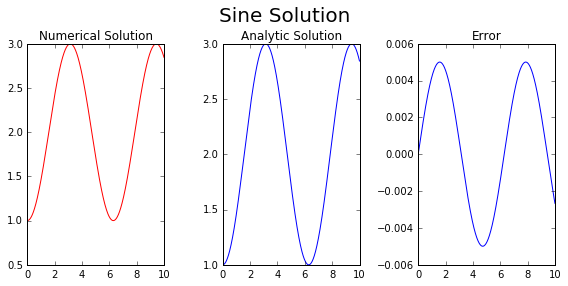
\includegraphics[scale=0.5]{sine_wave}
\caption{Python output: Numerical (left), Analytic (middle) and error(right) for $y'=\sin(x)$ Equation \ref{ODE_sine} with h=0.01}
\label{Sine wave ODE}
\end{figure}

\subsubsection{Simple example problem population growth $y^{'}=\ve y. $ }

\begin{example}
Simple population growth can be describe as a first order differential equation of the form: \begin{equation}\label{ODE_Growth} y^{'}=\ve y. \end{equation}
This has an exact solution of 
\[ y=Ce^{\ve x}. \]
Given the initial condition of  condition
\[y(0)=1\]
and a rate of change of
\[ \ve=0.5\]
the analytic solution is
\[ y=e^{0.5x}.\]

\end{example}

\begin{example} Applying the Euler formula to the first order equation
(\ref{ODE_Growth})
\[ y^{'} = 0.5y \]
is approximated by
\[\frac{w_{i+1}-w_i}{h}=0.5w_i. \]
Rearranging the equation gives the difference equation
\[w_{i+1}=w_i+h(0.5w_i). \]
The Python code below and the output is plotted in Figure \ref{GROWTH ODE Figure}.

\begin{lstlisting}[language=Python, caption=Python Numerical and Analytical Solution of Eqn \ref{ODE_Growth} ]
# Numerical solution of a differential equation
import numpy as np
import math 
import matplotlib.pyplot as plt

h=0.01
tau=0.5
a=0
b=10

N=int((b-a)/h)
w=np.zeros(N)
x=np.zeros(N)
Analytic_Solution=np.zeros(N)

Numerical_Solution[0]=1
x[0]=0
w[0]=1

for i in range (1,N):
    w[i]=w[i-1]+dx*(tau)*w[i-1]
    x[i]=x[i-1]+dx
    Analytic_Solution[i]=math.exp(tau*x[i])


fig = plt.figure(figsize=(8,4))
# --- left hand plot
ax = fig.add_subplot(1,3,1)
plt.plot(x,w,color='red')
#ax.legend(loc='best')
plt.title('Numerical Solution')

# --- right hand plot
ax = fig.add_subplot(1,3,2)
plt.plot(x,Analytic_Solution,color='blue')
plt.title('Analytic Solution')

#ax.legend(loc='best')
ax = fig.add_subplot(1,3,3)
plt.plot(x,Analytic_Solution-Numerical_Solution,color='blue')
plt.title('Error')

# --- title, explanatory text and save
fig.suptitle('Exponential Growth Solution', fontsize=20)
plt.tight_layout()
plt.subplots_adjust(top=0.85)
\end{lstlisting}
\end{example}

\begin{figure}[H]
\centering
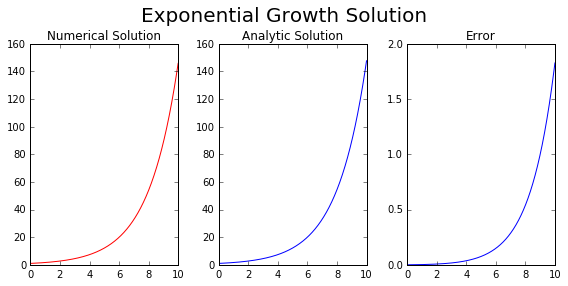
\includegraphics[scale=0.5]{ODE_Growth}
\caption{Python output: Numerical (left), Analytic (middle) and error(right) for $y^{'}=\ve y$  Eqn \ref{ODE_Growth} with h=0.01 and $\ve=0.5$}
\label{GROWTH ODE Figure}
\end{figure}

\subsubsection{Example of exponential growth with a wiggle}

\begin{example}
An extension of the exponential growth differential equation includes a sinusoidal component 
\begin{equation}\label{ODE_Growth_wiggle} y^{'}=\ve (y+y \sin(x)). \end{equation}
This complicates the exact solution but the numerical approach is more or less the same.
The difference equation is 
\[w_{i+1}=w_i+h(0.5w_i+w_i\sin(x_i)). \]
Figure \ref{GROWTH ODE WIGGLE} illustrates the numerical solution of the differential equation.

\begin{figure}[H]
\centering
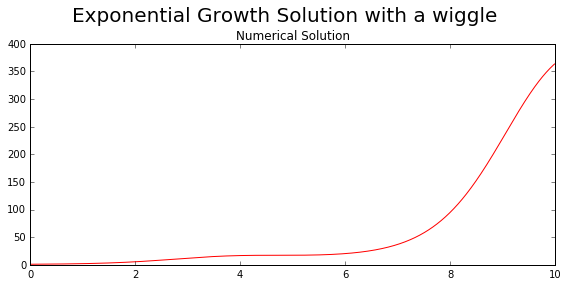
\includegraphics[scale=0.5]{ODE_Growth_with_a_wiggle}
\caption{Python output: Numerical solution for $y^{'}=\ve (y+y sin(x))$ Equation \ref{ODE_Growth_wiggle} with h=0.01 and $\ve=0.5$}
\label{GROWTH ODE WIGGLE}
\end{figure}

\end{example}

\subsection{Theorems about Ordinary Differential Equations}
\begin{definition}
A function $f(t,y)$ is said to satisfy a \textbf{\addtoindex{Lipschitz Condition}} in the variable $y$ on 
the set $D \subset R^2$ if a constant $L>0$ exist with the property that
\[|f(t,y_1)-f(t,y_2)| < L|y_1-y_2|, \]
whenever $(t,y_1),(t,y_2) \in D$.  The constant L is call the \addtoindex{Lipschitz Condition}
of $f$.
\end{definition}
\begin{definition}
A set $D\subset R^2$ is said to be convex if whenever $(t_1,y_1),(t_2,y_2)$ belong
to $D$ the point $((1-\lambda)t_1+\lambda t_2, (1-\lambda)y_1+\lambda y_2)$ also
belongs in $D$ for each $\lambda \in [0,1]$.
\end{definition}
\begin{theorem}
Suppose $f(t,y)$ is defined on a convex set $D \subset R^2$. If a constant
$L>0$ exists with
\[\left|\frac{\partial f(t,y)}{\partial y}\right|\leq L, \]
then $f$ satisfies a \addtoindex{Lipschitz Condition} an $D$ in the variable $y$ with
Lipschitz constant L.
\end{theorem}
\begin{theorem}
Suppose that
$D= \{(t,y) | a\leq t \leq b, -\infty <y < \infty \},$
and $f(t,y)$ is continuous on $D$ in the variable $y$ then the initial value
problem has a unique solution $y(t)$ for $a\leq t \leq b$.
\end{theorem}
\begin{definition}
The initial-value problem 
\[\frac{dy}{dt}=f(t,y), \ \ \ \ \  a\leq t \leq b,\]
with initial condition
\[y(a) = \alpha, \]
is said to be well posed if:
\begin{itemize}
\item
A unique solution $y(t)$ to the problem exists;
\item
For any $\varepsilon >0$ there exists a positive constant $k(\varepsilon)$
with the property that whenever $|\varepsilon_0| < \varepsilon$ and with
$|\delta(t)| \varepsilon$ on $[a,b]$ a unique solution $z(t)$ to the problem
\begin{equation} 
\label{perturbed}
\frac{dz}{dt}=f(t,z)+\delta(t), \ \ \  a\leq t \leq b, \end{equation}

\[z(a)=\alpha +\varepsilon_0, \]
exists with
\[ |z(t) - y(t) | < k(\varepsilon)\varepsilon. \]
The problem specified by (\ref{perturbed}) is called a perturbed problem associated
with the original problem.
\end{itemize}
It assumes the possibility of an error $\delta(\varepsilon)$ being introduced to
the statement of the differential equation as well as an error $\varepsilon_0$
being present in the initial condition.

\end{definition}
\begin{theorem}
Suppose $D= \{(t,y) | a\leq t \leq b, -\infty <y < \infty \}$.
If $f(t,y)$ is continuous and satisfies a \addtoindex{Lipschitz Condition} in the variable y on
the set $D$, then the initial value problem 
\[\frac{dy}{dt}=f(t,y), \ \ \  a\leq t \leq b,\]
with initial condition
\[y(a) = \alpha, \]
is well-posed.
\end{theorem}
\begin{example}
\[y^{'}(x)=-y(x)+1, \ \ \ \ 0\leq x \leq b, \ \ \ \ y(0)=1 \]
has the solution $y(x)=1$. The perturbed problem
\[z^{'}(x)=-z(x)+1, \ \ \ \ 0\leq x \leq b, \ \ \ \ z(0)=1+\va, \]
has the solution $z(x)=1+\va e^{-x}$ $x \leq 0$.\\
Thus 
\[y(x)-z(x)=-\va e^{-x} \]
\[|y(x)-z(x)|\leq |\va| \ \ \ \ x \geq 0 \]
Therefore the problem is said to be stable. This is illustrated in Figure \ref{Stable ODE}. 
\begin{figure}[H]
\centering
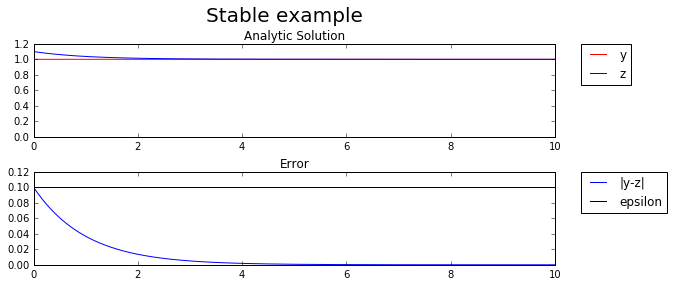
\includegraphics[scale=0.4]{Stable_example}
\caption{Python output: Illustrating Stability $y^{'}(x)=-y(x)+1$ with the initial condition $y(0)=1$ and $z^{'}(x)=-z(x)+1$ with the initial condition $z(0)=1+\va$, $\va=0.1$}
\label{Stable ODE}
\end{figure}

\end{example}

\section{One-Step Methods}
Dividing $[a,b]$ in to N subsections
such that we now have N+1 points of equal spacing $h=\frac{b-a}{N}$. This gives
the formula $t_i=a+ih$ for $i=0,1,...,N$.  
One-Step Methods for \addtoindex{Ordinary Differential Equation}'s only use one previous point to get
the approximation for the next point.  The initial condition gives $y(a=t_0)=\alpha$, this gives the starting point of our one step method.  The general formula
for One-step methods is 
\[ w_{i+1}=w_i+h\Phi(t_i,w_i,h), \] 
where $w_i$ is the approximated solution of the \addtoindex{Ordinary Differential Equation} at the point $t_i$
\[w_i\approx y_i.\]

\subsection{Euler's Method}
The simplest example of a one step method is Euler. The derivative is replaced
by the Euler approximation. The \addtoindex{Ordinary Differential Equation}
\[ \frac{dy}{dt}=f(t,y), \]
is discretised
\[\frac{y_i-y_{i-1}}{h}=f(t_{i-1},y_{i-1}) +T\]
T is the truncation error.\\
\begin{example}
Consider the Initial Value Problem
\[y^{'} = -\frac{y^2}{1+t}, \ \ \ a=0\leq t \leq b=0.5, \]
with the initial condition $y(0)=1$
the Euler approximation is
\[w_{i+1}=w_i -\frac{hw_i^2}{1+t_i}, \]
where $w_i$ is the approximation of $y$ at $t_i$.\\
Solving, let $t_i=ih$ where $h=0.05$, from the initial condition we have
$w_0=1$
at $i=0$ our method is 
\[w_1=w_0-\frac{0.05w^2_0}{1+t_0}=1-\frac{0.05}{1+0}=0.95 \]
and so forth, each approximation $w_i$ requiring the previous, thus creating a 
sequence starting at $w_0$ to $w_n$. The Table below show the numerical approximation for 10 steps.
\begin{center}
\begin{tabular}{ c| c |c }
  i& $t_i$& $w_i$\\
  \hline
 0 & $0$  & 1 \\  
 1 & $0.05$  & 0.95 \\  
 2 & $0.1$  & 0.90702381 \\  
 3 & $0.15$  & 0.86962871 \\  
 4 & $0.2$  & 0.8367481 \\  
 5 & $0.25$  & 0.80757529 \\  
 6 & $0.3$  & 0.78148818 \\  
 7 & $0.35$  & 0.7579988 \\  
 8 & $0.4$  & 0.73671872 \\  
 9 & $0.45$  & 0.71733463  
\end{tabular}
\end{center}
\end{example}

\begin{lemma}
\label{lemma 1}
For all $ x \geq 0.1$ and any positive m we have \[0\leq (1+x)^m \leq e^{mx}.\]
\end{lemma}

\begin{lemma}
\label{lemma 2}
If s and t are positive real numbers $\{a_i\}_{i=0}^{N}$ is a sequence satisfying $\displaystyle a_0 \geq \frac{-t}{s}$ and $a_{i+1} \leq (1+s)a_i +t $
then,
\[a_{i+1} \leq e^{(i+1)s}\left(a_0+\frac{t}{s}\right)-\frac{t}{s}. \] 
\end{lemma}
\begin{theorem}
\label{Euler bound}
Suppose $f$ is continuous and satisfies a \addtoindex{Lipschitz Condition} with constant
L on $D=\{(t,y)|a\leq t \leq b, -\infty < y < \infty \}$ and that a constant $M$
exists with the property that 
\[ |y^{''}(t)|\leq M. \]
Let $y(t)$ denote the unique solution of the \addtoindex{Initial Value Problem}
\[ y^{'}=f(t,y), \ \ \ a\leq t \leq b, \ \ \ y(a)=\alpha, \]
and $w_0,w_1,...,w_N$ be the approx generated by the Euler method for some
positive integer $N$.  Then for $i=0,1,...,N$
\[ |y(t_i)-w_i| \leq \frac{Mh}{2L}|e^{L(t_i-a)}-1|. \]
\end{theorem}
\begin{proof}
When $i=0$ the result is clearly true since $y(t_0)=w_0=\alpha$.
From Taylor we have,
\[y(t_{i+1})=y(t_i)+hf(t_i,y(t_i))+\frac{h^2}{2}y^{''}(\xi_i), \]
where $x_i \geq \xi_i \geq x_{i+1}$, and from this we get the Euler approximation
\[w_{i+1}=w_i + hf(t_i,w_i). \]
Consequently we have
\[y(t_{i+1})-w_{i+1}=y(t_i)-w_i+h[f(t_i,y(t_i))-f(t_i,w_i)]+\frac{h^2}{2}y^{''}(\xi_i), \]
and
\[|y(t_{i+1})-w_{i+1}|\leq |y(t_i)-w_i|+h|f(t_i,y(t_i))-f(t_i,w_i)|+\frac{h^2}{2}|y^{''}(\xi_i)|. \]
Since f satisfies a \addtoindex{Lipschitz Condition} in the second variable with constant L
and $|y^{''}|\leq M$ we have
\[|y(t_{i+1})-w_{i+1}|\leq (1+hL)|y(t_i)-w_i|+\frac{h^2}{2}M. \]
Using Lemma \ref{lemma 1} and \ref{lemma 2} and letting $a_j=(y_j-w_j)$ for each
$j=0,..,N$ while $s=hL$ and $t=\frac{h^2M}{2}$ we see that
\[|y(t_{i+1}-w_{i+1}|\leq e^{(i+1)hL}(|y(t_0)-w_0|+\frac{h^2M}{2hL}) -\frac{h^2M}{2hL}. \]
Since $w_0-y_0=0$ and $(i+1)h=t_{i+1}-t_0=t_{i+1}-a$ we have
\[ |y(t_i)-w_i| \leq \frac{Mh}{2L}|e^{L(t_i-a)}-1|, \]
for each $i=0,1,..N-1$.
\end{proof}
\begin{example}
\[y^{'}=y-t^2+1, \ \ \ 0 \leq t \leq 2, \ \ \ y(0)=0.5, \]
the Euler approximation is
\[w_{i+1} = w_i + h(w_i-t_i^2+1) \]
choosing $h=0.2$, $t_i=0.2i$ and $w_0=0.5$. \\
$f(t,y)=y-t^2+1$
\[\frac{\partial f}{\partial y}=1 \]
so $L=1$. The exact solution is $y(t)=(t+1)^2-\frac{1}{2}e^t$ from this we have
\[y^{''}(t) = 2-0.5e^t, \]
\[|y^{''}(t)| \leq 0.5e^2-2, \ \ t\in[0,2].\]
Using the above inequality we have we have
\[|y_i-w_i| \leq \frac{h}{2}(0.5e^2-2)(e^{t_i}-1).\]
Figure \ref{UpperBound Figure} illustrates the upper bound of the error and the actual error.

\begin{figure}[H]
\centering
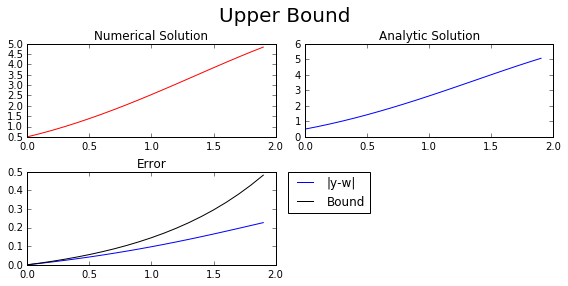
\includegraphics[scale=0.5]{UpperBound}
\caption{Python output: Illustrating upper bound $y^{'}=y-t^2+1$ with the initial condition $y(0)=0.5$ }
\label{UpperBound Figure}
\end{figure}
\end{example}
Euler method is a typical one step method, in general such methods are given by
function $\Phi(t,y;h;f)$. Our initial condition is $w_0=y_0$, for $i=0,1,..$
\[w_{i+1}=w_i+h\Phi(t_i,w_i:h:f)\]
with $t_{i+1}=t_i+h$.\\
In the Euler case $\Phi(t,y;h;f)=f(t,y)$ and is of order $1$.\\
Theorem \ref{Euler bound} can be extend to higher order one step methods with the variation 
\[ |y(t_i)-w_i| \leq \frac{Mh^p}{2L}|e^{L(t_i-a)}-1| \]
where $p$ is the order of the method.
\begin{definition}
The difference method $w_0=\alpha$
\[w_{i+1}=w_i+h\Phi(t_i,w_i),\]
for $i=0,1,...,N-1$ has a local truncation error given by
\begin{eqnarray*}
\tau_{i+1}(h) &=&\frac{y_{i+1}-(y_i+h\Phi(t_i,y_i))}{h},\\ 
&=&\frac{y_{i+1}-y_{i}}{h} -\Phi(t_i,y_i),
\end{eqnarray*}
for each $i=0,..,N-1$ where as usual $y_i=y(t_i)$ denotes the exact solution
at $t_i$.
\end{definition}
For Euler method the local truncation error at the ith step for the problem
\[ y^{'} = f(t,y), \ \ \ a\leq t \leq b, \ \ y(a)=\alpha, \]
is
\[\tau_{i+1}(h) =\frac{y_{i+1}-y_{i}}{h} -f(t_i,y_i), \]
for $i=0,..,N-1$.\\
But we know Euler has \[\tau_{i+1}=\frac{h}{2}y^{''}(\xi_i), \ \ \xi_i \in (t_i,t_{i+1}),\]
When $y^{''}(t)$ is known to be bounded by a constant M on $[a,b]$ this implies
\[|t_{i+1}(h)| \leq \frac{h}{2}M \sim O(h). \]
$O(h)$ indicates a linear order of error. The higher the order the more accurate the method.
\newpage
\section{Problem Sheet}
\begin{enumerate}
\item
Show that the following functions satisfy the Lipschitz condition on $y$ on the indicated set $D$:
\begin{enumerate}
\item
$f(t,y)=ty^3,$  $D=\{(t,y);-1\leq t \leq 1, 0\leq y \leq 10\};$
\item 
$f(t,y)=\frac{t^2y^2}{1+t^2},$  $D=\{(t,y);0\leq t, -10\leq y \leq 10 \}.$

\end{enumerate}
\item
Apply Euler's Method to approximate the solution of the given initial value problems using the indicated number of time steps. Compare the approximate solution with the given exact solution, and compate the actual error with the theoretical error
\begin{enumerate}
\item
$y'=t-y, \ \ (0\leq t \leq 4)$\\
with the initial condition $y(0)=1,$\\
$N=4$, 
$y(t)=2e^{-t}+t-1,$\\

The Lipschitz constant is determined on  $D=\{(t,y);0\leq t \leq 4, y\in \rm I\!R \}.$
\item 
$y'=y-t, \ \ (0\leq t \leq 2)$\\
with the initial condition $y(0)=2,$\\
$N=4$, 
$y(t)=e^{t}+t+1$.\\

The Lipschitz constant is determined on  $D=\{(t,y);0\leq t \leq 2, y\in \rm I\!R \}.$
\end{enumerate}

\end{enumerate}
\newpage
\chapter{Higher Order Methods}
\section{Higher order Taylor Methods}
The Taylor expansion
\[ y(t_{i+1})=y(t_i)+h y^{'}(t_i)+\frac{h^2}{2}y^{'}(t_i)+..+\frac{h^{n+1}}{(n+1)!}y^{n+1}(\xi_i) \]
can be used to design more accurate higher order methods. 
By differentiating the original \addtoindex{Ordinary Differential Equation} $y^{'}=f(t,y)$  higher ordered can be derived 
method it requires the function to be continuous and differentiable.\\
In the general case of Taylor of order n:
\[ w_0=\alpha \]
\[ w_{i+1} = w_i + hT^n(t_i,w_i), \mbox{   for   } \ i=0,...,N-1, \]
where
\begin{equation} T^{n}(t_i,w_i) = f(t_i,w_i)+\frac{h}{2}f'(t_i,w_i)+...\frac{h^{n-1}}{n!}f^{n-1}(t_i,w_i). \end{equation}
\begin{example}
Applying the general Taylor method to create methods of order two and four to
the initial value problem
\[y^{'}=y-t^2+1, \ \ \ 0\leq t \leq 2, \ \ \ y(0)=0.5, \]
from this we have 
\[ f^{'}(t,y(t)) = \frac{d}{dt}(y-t^2+1) = y'-2t=y-t^2+1-2t, \]
\[ f^{''}(t,y(t)) = y-t^2-2t-1, \]
\[ f^{'''}(t,y(t)) = y-t^2-2t-1. \]
From these derivatives we have
\begin{eqnarray*}
T^{2}(t_i,w_i)&=&f(t_i,w_i)+\frac{h}{2}f^{'}(t_i,w_i)\\
&=&w_i-t_i^2+1+\frac{h}{2}(w_i-t_i^2-2t_i+1)\\
&=&\left(1+\frac{h}{2}\right)(w_i-t_i^2-2t_i+1)-ht_i
\end{eqnarray*}
and
\begin{eqnarray*}
T^{4}(t_i,w_i)&=&f(t_i,w_i)+\frac{h}{2}f^{'}(t_i,w_i)\\
& &+\frac{h^2}{6}f^{''}(t_i,w_i)+\frac{h^3}{24}f^{''}(t_i,w_i)\\
&=&\left(1+\frac{h}{2}+\frac{h^2}{6}+\frac{h^3}{24}\right)(w_i-t_i^2)\\
& &-\left(1+\frac{h}{3}+\frac{h^2}{12}\right)ht_i\\
& & +1+\frac{h}{2}-\frac{h^2}{6}-\frac{h^3}{24}
\end{eqnarray*}
From these equations we have,
Taylor of order two
\[w_0=0.5\]
\[w_{i+1}=w_i+h\left[\left(1+\frac{h}{2}\right)(w_i-t_i^2-2t_i+1)-ht_i
\right] \]
and Taylor of order 4
\begin{eqnarray*}w_{i+1}&=&w_i+h\left[\left(1+\frac{h}{2}+\frac{h^2}{6}+\frac{h^3}{24}\right)(w_i-t_i^2)\right.\\
& &\left.-\left(1+\frac{h}{3}+\frac{h^2}{12}\right)ht_i
 +1+\frac{h}{2}-\frac{h^2}{6}-\frac{h^3}{24}
\right] \end{eqnarray*}
The local truncation error for the 2nd order method is 
\[\tau_{i+1}(h) = \frac{y_{i+1}-y_i}{h} -T^2(t_i,y_i) = \frac{h^2}{6}f^2(\xi_i,y(x_i))\]
where $\xi \in (t_i,t_{i+1})$.
\end{example}
In general if $y \in C^{n+1}[a,b]$
\[\tau_{i+1}(h)=\frac{h^n}{(n+1)!}f^{n}(\xi_i,y(\xi_i))~O(h^n). \]
The issue is that for every differential equation a new method has be to derived.


\chapter{Runge--Kutta Method}
The \addtoindex{Runge-Kutta method} (RK) method is closely related to the Taylor series expansions but no differentiation of $f$ is necessary.\\
All RK methods will be written in the form
\begin{equation}
\label{RK A}
w_{n+1} =w_n +hF(t,w,h;f), \ \ \ n\geq 0.
\end{equation}
The truncation error for (\ref{RK A}) is defined by
\[
T_{n}(y) =y(t_{n+1})-y(t_n) -hF(t_n,y(t_n),h;f) 
\]
where the error is written as $\tau_n(y)$ 
\[ T_n=h\tau_n(y).\]
Rearranging we get
\[
y(t_{n+1})=y(t_n) -h F(t_n,y(t_n),h;f) +
h\tau_n(y).\]


\begin{theorem} \label{RK_Theorem}
Suppose f(t,y) and all its partial derivatives of order less than or equal to
n+1 are continuous on $D=\{(t,y)|a\leq t \leq b, c \leq y \leq d \}$ and let 
$(t_0,y_0)\in D$ for every $(t,y)\in D$, $\exists \ \ \xi \in (t,t_0)$ and $\mu \in (y,y_0)$ with
\[f(t,y) = P_n(t,y) + R_n(t,y) \]
where
\begin{eqnarray*}
 P_n(t,y) &=& f(t_0,y_0)+\left[(t-t_0)\frac{\partial f}{\partial t}(t_0,y_0)+(y-y_0)\frac{\partial f}{\partial y}(t_0,y_0) \right]\\
& & + \left[\frac{(t-t_0)^2}{2}\frac{\partial^2 f}{\partial t^2}(t_0,y_0)+(y-y_0)(t-t_0)\frac{\partial^2 f}{\partial y\partial t}(t_0,y_0)\right. \\
& & +\left. \frac{(y-y_0)^2}{2}\frac{\partial^2 f}{\partial y^2}(t_0,y_0) \right]\\
& & +...+\\
& & + \left[\frac{1}{n!}\sum_{j=0}^n\left(\begin{array}{c}n \\ j \end{array}\right)(t-t_0)^{n-j}(y-y_0)^j\frac{\partial^n f}{\partial y^j\partial t^{n-j}}(t_0,y_0)  \right]
\end{eqnarray*}
and
\begin{eqnarray*}\begin{aligned}R_n(t,y) = \\\left[\frac{1}{(n+1)!}\sum_{j=0}^{n+1}\left(\begin{array}{c}n+1 \\ j \end{array}\right)(t-t_0)^{n+1-j}(y-y_0)^j\frac{\partial^{n+1} f}{\partial y^j\partial t^{n+1-j}}(\xi,\mu)  \right]\end{aligned}
\end{eqnarray*}
\end{theorem}
\section{Derivation of Second Order Runge Kutta}
Consider the explicit one-step method\\
\begin{equation}
\frac{w_{i+1}-w_i}{h}=F(f,t_i,w_i,h)
\end{equation}
with
\begin{equation}
F(f,t,y,h)=a_0k_1+a_1k_2,
\end{equation}
\begin{equation}
F(f,t,y,h)=a_0f(t,y)+a_1f(t+\alpha_1,y+\beta_1),
\end{equation}
where $a_0+a_1=1.$\\
\textbf{There is a free parameter in the derivation of the Runge Kutta method for this reason $a_0$ must be choosen}

Deriving the second order \addtoindex{Runge-Kutta method} by using Theorem \ref{RK_Theorem} to determine values for values  $a_1,\alpha_1$ and $\beta_1$ with the property that $a_1f(t+\alpha_1,y+\beta_1)$ approximates the second order Taylor
\[f(t,y)+\frac{h}{2}f^{'}(t,y) \]
with error no greater than than $O(h^2)$, the local truncation error for
the Taylor method of order two.\\
Using
\[f^{'}(t,y)=\frac{\partial f}{\partial t}(y,t)+\frac{\partial f}{\partial y}(t,y).y^{'}(t), \]
the second order Taylor can be re-written as
\begin{equation}
\label{RKA}
f(t,y)+\frac{h}{2}\frac{\partial f}{\partial t}(y,t)+\frac{h}{2}\frac{\partial f}{\partial y}(t,y).f(t,y).
\end{equation}
Expanding $a_1f(t+\alpha_1,y+\beta_1)$ in its Taylor polynomial of degree one about
$(t,y)$ gives
\begin{equation}
\label{RKB}
a_1f(t+\alpha_1,y+\beta_1)= a_1 f(t,y) +a_1 \alpha_1 \frac{\partial f}{\partial t}(t,y)+a_1 \beta_1\frac{\partial f}{\partial y}+a_1R_1(t+\alpha_1,y+\beta_1)
\end{equation}
where
\[ R_1(t+\alpha_1,y+\beta_1)=\frac{\alpha_1^2}{2}\frac{\partial^2 f}{\partial t ^2}(\xi,\mu)
+\alpha_1 \beta_1 \frac{\partial^2 f}{\partial t \partial y}(\xi,\mu)
+\frac{\beta_1^2}{2}\frac{\partial^2 f}{\partial y^2} (\xi,\mu),
\]for some $\xi \in [t,t+\alpha_1]$ and $\mu \in [y,y+\beta_1]$.\\
Matching the coefficients and its derivatives in eqns (\ref{RKA}) and (\ref{RKB}) 
gives the equations
\[f(t,y): a_1=1\]
\[\frac{\partial f }{\partial t}(t,y): a_1\alpha_1=\frac{h}{2} \]
and
\[\frac{\partial f }{\partial y}(t,y): a_1\beta_1=\frac{h}{2}f(t,y). \]
\subsection{Runge Kutta second order: Midpoint method}
Choosing $a_0=0$ gives the unique values $a_1=1$, $\alpha_1=\frac{h}{2}$ and $\beta_1=\frac{h}{2}f(t,y)$
so
\[T^{2}(t,y) = f(t+\frac{h}{2},y+\frac{h}{2}f(t,y))-R_1(t+\frac{h}{2},y+\frac{h}{2}f(t,y))
\]
and from
\[ R_1(t+\frac{h}{2},y+\frac{h}{2}f(t,y))=\frac{h^2}{8}\frac{\partial^2 f}{\partial t ^2}(\xi,\mu)
+\frac{h^2}{4} \frac{\partial^2 f}{\partial t \partial y}(\xi,\mu)
+\frac{h^2}{8}g(t,y)^2\frac{\partial^2 f}{\partial y^2} (\xi,\mu),
\]for some $\xi \in [t,t+\frac{h}{2}]$ and $\mu \in [y,y+\frac{h}{2}f(t,y)]$.\\
If all the second-order partial derivatives are bounded then
\[ R_1(t+\frac{h}{2},y+\frac{h}{2}f(t,y)) \sim O(h^2). \]
The Midpoint second order Runge-Kutta for the initial value problem
\[y'=f(t,y)\] 
with the initial condition $y(t_0)=\alpha$ is given by
\[w_0=\alpha, \]
\[w_{i+1}=w_i+hf(t_i+\frac{h}{2},y_i+\frac{h}{2}f(t_i,w_i)), \]
with an error of order $O(h^2)$.
The Figure \ref{Modified Euler Figure} illustrates the solution to the  $y^{'}=-xy$
\begin{figure}[H]
\centering
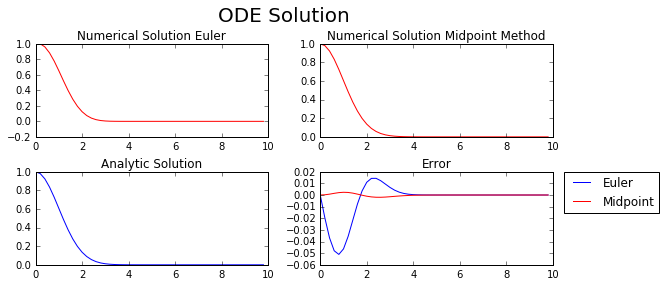
\includegraphics[scale=0.5]{ODE_solution_Euler_Modified}
\caption{Python output: Illustrating upper bound $y^{'}=-xy$ with the initial condition $y(0)=1$ }
\label{Modified Euler Figure}
\end{figure}
for each $i=0,1,...N-1.$

\subsection{2nd Order Runge Kutta $a_0=0.5$: Heun's method}
Choosing $a_0=0.5$ gives the unique values $a_1=0.5$, $\alpha_1=h$ and $\beta_1=hf(t,y)$
such that 
\[T^{2}(t,y)=F(t,y) = 0.5 f(t,y)+0.5 f(t+h,y+hf(t,y))-R_1(t+h,y+hf(t,y))
\]
and the error value from
\[ R_1(t+h,y+hf(t,y))=\frac{h^2}{2}\frac{\partial^2 f}{\partial t ^2}(\xi,\mu)
+h^2 \frac{\partial^2 f}{\partial t \partial y}(\xi,\mu)
+\frac{h^2}{2}f(t,y)^2\frac{\partial^2 f}{\partial y^2} (\xi,\mu),
\]for some $\xi \in [t,t+h]$ and $\mu \in [y,y+hf(t,y)]$.\\

Thus Heun's second order Runge-Kutta for the initial value problem
\[y'=f(t,y)\] 
with the initial condition $y(t_0)=\alpha$ is given by
\[w_0=\alpha, \]
\[w_{i+1}=w_i+\frac{h}{2}[f(t_i,w_i)+f(t_i+h,y_i+hf(t_i,w_i))] \]
with an error of order $O(h^2)$.\\
For ease of calculation this can be rewritten as:
\[k_1=f(t_i,w_i),\]
\[k_2=f(t_i+h,w_i+hk_1),\]
\[w_{i+1}=w_i+\frac{h}{2}[k_1+k_2]. \]

\section{Third Order Runge Kutta methods}
Higher order methods are derived in a similar fashion.
For the Third Order Runge Kutta methods 
\begin{equation}
\frac{w_{i+1}-w_i}{h}=F(f,t_i,w_i,h)
\end{equation}
with
\begin{equation}
F(f,t,w,h)=a_0k_1+a_1k_2+a_2k_3
\end{equation}
where 
\[a_0+a_1+a_2=1\] 
and
\[k_1=f(t_i,w_i)\]
\[k_2=f(t_i+\alpha_1h,t_i+\beta_{11}k_1)\]
\[k_3=f(t_i+\alpha_2h,t_i+\beta_{21}k_1+\beta_{22}k_2)).\]
The values of $a_0$, $a_1$, $a_2$, $\alpha_1,\alpha_2$, $\beta_{11}$,$\beta_{21}$, $\beta_{22}$ are derived by group the Taylor expansion,
\begin{eqnarray}{lcl} y_{i+1}&=&y_{i}+hf(t_{i},y_{i})+{\frac {h^{2}}{2}}(f_{t}+f_{y}f)_{(t_{i},y_{i})}\\
& &+{\frac {h^{3}}{6}}\left(f_{tt}+2f_{ty}f+f_{t}f_{y}+f_{yy}f^{2}+f_{y}f_{y}f\right)_{(t_{i},y_{i})}\\
& &+O(h^{4}),\end{eqnarray}
with the 3rd order expand form:
\[ y_{i+1}=y_{i}+ha_{1}f(t_{i},y_{i})+ha_{2}(f+\alpha_{1}hf_{t}+\beta_{11}hf_{y}f\]\[+{\frac {h^{2}}{2}}(f_{tt}\alpha_{1}^{2}+f_{yy}\beta_{11}^{2}f^{2}+2f_{ty}\alpha_{1}\beta_{11}f)+O_{2}(h^{3}))\]
\[+ha_{3}(f+\alpha_{2}hf_{t}+f_{y}\left(\beta_{21}hf+\beta_{22}h(f+\alpha_{1}hf_{t}+\beta_{11}hf_{y}f+O_{3}(h^{2}))\right)\] 
\[+{\frac {1}{2}}(f_{tt}(\alpha_{2}h)^{2}+f_{yy}h^{2}(\beta_{21}f+ \beta_{22}(f+\underbrace {\alpha_{1}hf_{t}+\beta_{11}hf_{y}f+O_{4}(h^{2})} _{O_{5}(h)}))^{2}\]
 \[+2f_{ty}\alpha_{2}h^{2}(\beta_{21}f+\beta_{22}(f+\underbrace {\alpha_{1}hf_{t}+\beta_{11}hf_{y}f+O_{4}(h^{2})} _{O_{5}(h)})))).\]
 This results in 8 equations with 8 unknowns, but only 6 of these equations are independent. For this reason the are two free parameters to choose.

For example, we can choose that \[\alpha_{2}=1,\beta_{11}=\frac{1}{2},\]then we obtain the following difference equation.
\[ w_{i+1}=w_{i}+{\frac {h}{6}}(k_{1}+4k_{2}+k_{3})\]
where
\[k_{1}=f(t_{i},w_{i}),\]
\[ k_{2}=f(t_{n}+1/2h,w_{n}+1/2hk_{1}),\]
\[ k_{3}=f(t_{n}+h,w_{n}-hk_{1}+2hk_{2}).\]

\section{Runge Kutta fourth order}
\[w_0 = \alpha, \]
\[k_1 = hf(t_i,w_i), \]
\[k_2 = hf(t_i+\frac{h}{2},w_i+\frac{1}{2}k_1), \]
\[k_3 = hf(t_i+\frac{h}{2},w_i+\frac{1}{2}k_2), \]
\[k_4 = hf(t_{i+1},w_i+k_3), \]
\[w_{i+1}=w_{i}+\frac{1}{6}(k_1+2k_2+2k_3+k_4). \]
\begin{example}
Example Midpoint method
\[y^{'}=y-t^2+1 \ \ \ 0 \leq t \leq 2 \ \ \ y(0)=0.5, \]
\[N=10, \ \ \ t_i=0.2i, \ \ \ h=0.2, \]
\[w_0=0.5, \]
\begin{eqnarray*}
w_{i+1} &=& w_{i} + 0.2f(t_i+\frac{0.2}{2},w_i+\frac{0.2}{2}f(t_i,w_i))\\
 &=& w_{i} + 0.2f(t_i+0.1,w_i+0.1(w_i-t^2_i+1))\\
 &=& w_{i} + 0.2(w_i+0.1(w_i-t^2_i+1)-(t_i+0.1)^2+1)\\
\end{eqnarray*}
Example Runge Kutta fourth order method
\[y^{'}=y-t^2+1 \ \ \ 0 \leq t \leq 2 \ \ \ y(0)=0.5 \]
\[N=10 \ \ \ t_i=0.2i \ \ \ h=0.2 \]
\[w_0=0.5 \]
\begin{eqnarray*}
k_1&=&h(w_i-t_i^2+1)\\
k_2&=&h(w_i+\frac{1}{2}k_1-(t_i+\frac{h}{2})^2+1)\\
k_3&=&h(w_i+\frac{1}{2}k_2-(t_i+\frac{h}{2})^2+1)\\
k_4&=&h(w_i+\frac{1}{2}k_3-(t_i+h)^2+1)\\
w_{i+1} &=& w_{i} + \frac{1}{6}(k_1+2k_2+2k_3+k_4)
\end{eqnarray*}
\begin{figure}[H]
\centering
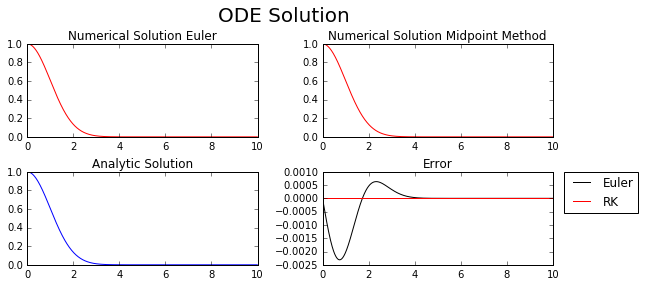
\includegraphics[scale=0.5]{ODE_solution_Euler_RK}
\caption{Python output: Illustrating upper bound $y^{'}=-xy$ with the initial condition $y(0)=1$ }
\label{RK vs Euler Figure}
\end{figure}
\begin{figure}[H]
\centering
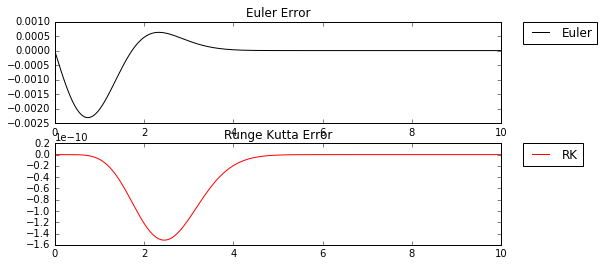
\includegraphics[scale=0.5]{ODE_error_RK_Euler}
\caption{Python output: Illustrating upper bound $y^{'}=-xy$ with the initial condition $y(0)=1$ }
\label{Modified Euler Figure}
\end{figure}
\end{example}
\section{Butcher Tableau}

Another way of representing a Runge Kutta method is called the Butcher tableau named after John C Butcher(31 March 1933).

\[ y_{i+1}=y_{i}+h\sum _{n=1}^{s}a_{n}k_{n},\] 
where

\[ {\begin{aligned}k_{1}&=f(t_{i},y_{i}),\\k_{2}&=f(t_{i}+\alpha_{2}h,y_{i}+h(\beta_{21}k_{1})),\\k_{3}&=f(t_{i}+\alpha_{3}h,y_{i}+h(\beta_{31}k_{1}+\beta_{32}k_{2})),\\&\ \ \vdots \\k_{s}&=f(t_{i}+\alpha_{s}h,y_{i}+h(\beta_{s1}k_{1}+\beta_{s2}k_{2}+\cdots +\beta_{s,s-1}k_{s-1})).\end{aligned}}\] 

These data are usually arranged in a mnemonic device, known as a Butcher tableau
\begin{center}
 \begin{tabular}{c| c c c c c} 
 0&  &  & & & \\ 
 $c_2$& $\beta_{21}$ &  & & & \\ 
 $c_3$& $\beta_{31}$ & $\beta_{31}$ & & & \\ 
 $\vdots $& $\vdots$ & $\vdots$  & & & \\ 
 
 $c_s$& $\beta_{s1}$ & $\beta_{s2}$ & $\cdots$& $\beta_{ss-1}$ & \\ 
 \hline
 & $a_{1}$  & $a_{2}$ & $\cdots$ &$a_{s-1}$ & $a_s$ \\ 
\end{tabular}
\end{center}
The method is consistent if 
\[\sum_{j}^{s-1} \beta_{sj}=c_s.\]
\subsection{Heun's Method}
The Butcher's Tableau for Heun's Method is:
\begin{center}
 \begin{tabular}{c| c c} 
 $0$&    &   \\ 
 $1$& $1$ &   \\ 
 \hline
 & $\frac{1}{2}$  & $\frac{1}{2}$   \\ 
\end{tabular}
\end{center}
\subsection{4th Order Runge Kutta}
The Butcher's Tableau for the 4th Order Runge Kutta is:
\begin{center}
 \begin{tabular}{c| c c c c} 
 $0$&    &  & & \\ 
 $\frac{1}{2}$& $\frac{1}{2}$ &  & & \\ 
 $\frac{1}{2}$& $0$ & $\frac{1}{2}$ & &  \\ 
 $1 $& $0$ & $0$  &$1$ &  \\ 
 \hline
 & $\frac{1}{6}$  & $\frac{2}{6}$ & $\frac{2}{6}$ &$\frac{1}{6}$  \\ 
\end{tabular}
\end{center}

\section{Convergence Analysis}
In order to obtain convergence of the general Runge Kutta we need to have the truncation
$\tau_n(y)\rightarrow0$ as $h \rightarrow 0$.  Since,
\[\tau(y)=\frac{y(t_{n+1})-y(t_n)}{h}-F(t_n,y(t_n),h;f), \]
we require,
\[F(x,y,h;f)\rightarrow y{'}(x)=f(x,y(x)). \]
More precisely define,
\[\delta(h)= \max_{a\leq t \leq b ; -\infty < y <\infty} |f(t,y)-F(t,y,h;f)|, \]
and assume,
\begin{equation}
\label{C}
 \delta(h) \rightarrow 0, \ \ \ \mbox{ as } h \rightarrow 0.
 \end{equation}
This is called the \underline{consistency condition} for the RK method.\\
We will also need a \addtoindex{Lipschitz Condition} on $F$:
\begin{equation}
\label{L}
|F(t,y,h;f)-F(t,z,h;f)|\leq |y-z|,
 \end{equation}
for all $a\leq t \leq b$ and $-\infty <y,z < \infty $ and small $h >0$.
\begin{example}
Looking at the midpoint method
\begin{eqnarray*}
|F(t,w,h;f)-F(t,z,h;f)| &=&
\left|f(t+\frac{h}{2},w+\frac{h}{2}f(t,w)) \right. \\
& & \left. -f(t+\frac{h}{2},z+\frac{h}{2}f(t,z) )
 \right|\\
&\leq& K \left| w-z +\frac{h}{2}[f(t,w)-f(t,z) ]\right|\\
&\leq &	K \left(1 +\frac{h}{2}K \right)|w-z|
\end{eqnarray*}
\end{example}
\begin{theorem}
Assume that the Runge Kutta method satisfies the \addtoindex{Lipschitz Condition}. Then
for the initial value problems
\[ y^{'}=f(x,y),\]
\[ y(x_0)=y_0. \]
The numerical solution $\{ w_n\}$ satisfies
\[ \max_{a\leq x\leq b}|y(x_n)-w_n| \leq e^{(b-a)L}|y_0-w_0|+\left[\frac{e^{(b-a)L}-1}{L} \right]\tau(h) \]
where
\[\tau(h) = \max_{a\leq x\leq b}|\tau_n(Y)|,\]
If the consistency condition 
\[ \delta(h) \rightarrow 0 \mbox{ as  } h\rightarrow 0, \]
where
\[\delta(h) = \max_{a \leq x \leq b}|f(x,y)-F(x,y;h;f)|. \]

\end{theorem}
\begin{proof}
Subtracting
\[ w_{n+1}=w_n +hF(t_n,w_n,h;f),\]
and
\[y( t_{n+1})=y(t_n) +hF(t_n,y(t_n),h;f)+h\tau_n(h),\]
we obtain
\[ e_{n+1}=e_n +h[F(t_n,w_n,h;f)-F(t_n,w_n,h;f)]+h\tau_n(h),\]
in which $e_n=y(t_n)-w_n$. Apply the \addtoindex{Lipschitz Condition} $L$ and the truncation
error we obtain
\[|e_{n+1}| \leq (1+hL)|e_n| + h \tau_n(h). \]
This nicely leads to the result.\\
In most cases it is known by direct computation that $\tau(Y) \rightarrow 0$ as $h \rightarrow 0$
an in that case convergence of $\{w_n \}$ and $y(t_n)$ is immediately proved.
\\
But all we need to know is that (\ref{C}) is satisfied .  To see this we write
\[\begin{array}{ccc}
h\tau_n &=& Y( t_{n+1})-Y(t_n) -hF(t_n,Y(t_n),h;f),\\
&=&hY^{'}(t_n)+\frac{h^{2}}{2}Y^{''}(\xi_n) -hF(t_n,Y(t_n),h;f),\\
h|\tau_n| &\leq& h\delta(h)+\frac{h^{2}}{2}|Y^{''}|.\\
|\tau_n| &\leq& \delta(h)+\frac{h}{2}|Y^{''}|.\\
\end{array}
\]
Thus $\tau(h) \rightarrow 0$ as $h \rightarrow 0$
\end{proof}
From this we have
\begin{corollary}
If the RK method has a truncation error $\tau(Y)=O(h^{m+1})$ then the rate of
convergence of $\{w_n\}$ to $Y(t)$ is $O(h^m)$.
\end{corollary}

\section{The choice of method and step-size}
An interesting question is since \addtoindex{Runge-Kutta method} is 4th order but requires 4 steps and Euler
only required 3 is it more beneficial to use a smaller h than a higher order method?\\
But this does lead us to the question of how do we define our h to maximize
the solution we have.\\
An ideal difference-equation method
\[w_{i+1}=w_i+h\phi(t_i,w_i,h) \ \ \ i=0,..,n-1 \]
for approximating the solution $y(t)$ to the \addtoindex{Initial Value Problem}
$ y^{'} = f(t,y)$ would have the property that given a tolerance $\varepsilon >0$
the minimal number of mesh points would be used to ensure that the global error
$|y(t_i)-w_i|$ would not exceed $\va$ for any $i=0,...,N.$\\
We do this by finding an appropriate choice of mesh points. Although we cannot 
generally determine the global error of a method there is a close relation between 
local truncation and global error.  By using methods of differing order we can predict the local truncation error and using this prediction choose a step size
that will keep global error in check.\\
Suppose we have two techniques
\begin{enumerate}
\item
An nth order Taylor method of the form
\[y(t_{i+1}) = y(t_i) +h\phi(t_i,y(t_i),h_i)+O(h^{n+1}) \]
producing approximations
\[w_0=\alpha \]
\[w_{i+1}=w_i +h\phi(t_i,w_i,h_i)\]
with local truncation $\tau_{i+1}=O(h^n).$
\item
An (n+1)st order Taylor of the form
\[y(t_{i+1}) = y(t_i) +h\psi(t_i,y(t_i),h_i)+O(h^{n+2}) \]
producing approximations
\[v_0=\alpha \]
\[v_{i+1}=v_i +h\psi(t_i,v_i,h_i)\]
with local truncation $\upsilon_{i+1}=O(h^{n+1}).$
\end{enumerate}
We first make the assumption that $w_i \approx y(t_i) \approx v_i$ and choose a fixed
step size to generate $w_{i+1}$ and $v_{i+1}$ to approximate $y(t_{i+1})$.  Then
\begin{eqnarray*}
\tau_{i+1} & = & \frac{y(t_{i+1})-y(t_i)}{h} - \phi(t_i,y(t_i),h) \\
& = &  \frac{y(t_{i+1})-w_i}{h} - \phi(t_i,w_i,h) \\
& = &  \frac{y(t_{i+1})-(w_i+h\phi(t_i,w_i,h)}{h}) \\
& = &  \frac{y(t_{i+1})-w_{i+1}}{h} 
\end{eqnarray*}
Similarly
\[ \Upsilon_{i+1} =\frac{y(t_{i+1})-v_{i+1}}{h} \]
As a consequence
\begin{eqnarray*}
\tau_{i+1} &=& \frac{y(t_{i+1})-w_{i+1}}{h} \\
 &=& \frac{(y(t_{i+1})-v_{i+1})+(v_{i+1}-w_{i+1})}{h} \\
 &=& \Upsilon_{i+1}(h)+\frac{(v_{i+1}-w_{i+1})}{h}. 
\end{eqnarray*}
But $\tau_{i+1}(h)$ is $O(h^n)$ and $\Upsilon_{i+1}(h)$ is $O(h^{n+1})$ so the 
significant factor of $\tau_{i+1}(h)$ must come from $\frac{(v_{i+1}-w_{i+1})}{h}$.  This gives us an easily computed approximation of $O(h^n)$ method.
\[\tau_{i+1} \approx \frac{(v_{i+1}-w_{i+1})}{h}.  \]
The object is not to estimate the local truncation error but to adjust step size to 
keep it within a specified bound.  To do this we assume that since $\tau_{i+1}(h)$ is $O(h^n)$ a number $K$ independent of $h$ exists with \[\tau_{i+1}(h) \approx Kh^n. \]
Then the local truncation error produced by applying the nth order method with a
new step size $qh$ can be estimated using the original approximations $w_{i+1}$ 
and $v_{i+1}$
\[\tau_{i+1}(qh) \approx K(qh)^n \approx q^n\tau_{i+1}(h) \approx \frac{q^n}{h}(v_{i+1}-w_{i+1}), \]
to bound $\tau_{i+1}(qh)$ by $\va$ we choose $q$ such that
\[\frac{q^n}{h}|v_{i+1}-w_{i+1}|\approx \tau_{i+1}(qh) \leq \va, \]
which leads to
\[ q \leq \left( \frac{\va h }{|v_{i+1}-w_{i+1}|}\right)^{\frac{1}{n}}, \]
which can be used to control the error.


\newpage
\section{Problem Sheet 2}
\begin{enumerate}
\item
Apply the Taylor method to approximate the solution of initial value problem
\[ y'=ty+ty^2, \ \ \ (0\leq t \leq 2), \ \ \ y(0)=\frac{1}{2} \]
using $N=4$ steps

\item
Apply the Midpoint Method to approximate the solution of the given initial value problems using the indicated number of time steps. Compare the approximate solution with the given exact solution
\begin{enumerate}
\item
$y'=t-y, \ \ (0\leq t \leq 4)$\\
with the initial condition $y(0)=1,$\\
$N=4$, 
$y(t)=2e^{-t}+t-1$\\

\item 
$y'=y-t, \ \ (0\leq t \leq 2)$\\
with the initial condition $y(0)=2,$\\
$N=4$, 
$y(t)=e^{t}+t+1$\\

\end{enumerate}
\item
Apply the 4th Order Runge Kutta Method to approximate the solution of the given initial value problems using the indicated number of time steps. Compare the approximate solution with the given exact solution
\begin{enumerate}
\item
$y'=t-y, \ \ (0\leq t \leq 4)$\\
with the initial condition $y(0)=1,$\\
$N=4$, 
$y(t)=2e^{-t}+t-1$\\

\item 
$y'=y-t, \ \ (0\leq t \leq 2)$\\
with the initial condition $y(0)=2,$\\
$N=4$, 
$y(t)=e^{t}+t+1$\\

\end{enumerate}
\item
Derive the difference equation for the Midpoint Runge Kutta method\\
\[ w_{n+1}=w_n+k_2\]
\[k_1=hf(t_n,w_n)\]
\[k_2=hf(t_n+\frac{1}{2}h,w_n+\frac{1}{2}k_1)\]
for dolving the ordinary differential equation
\[ \frac{dy}{dt}=f(t,y) \]
\[y(t_0)=y_0 \]
by using a formula of the form
\[w_{n+1}=w_n+ak_1+bk_2 \]
where $k_1$ is defined as above,
\[k_2=hf(t_n+\alpha h,w_n+\beta k_1)\]
and $a$, $b$, $\alpha$ and $\beta$ are constants are deteremined. Prove that $a+b=1$ and $b\alpha=b\beta=\frac{1}{2}$ and choose appropriate values to give the Midpoint Runge Kutta method.


\end{enumerate}
\newpage

\chapter{Multi-step Methods}
Methods using the approximation at more than one previous point to determine the
approx at the next point are called multi-step methods.
\begin{definition}
An m-step multi-step method for solving the \addtoindex{Initial Value Problem}
\[y^{'} = f(t,y) \ \ a\leq t \leq b \ \ y(a) =\alpha\]
is on whose difference equation for finding the approximation $w_{i+1}$ at the
mesh points $t_{i+1}$ can be represented by the following equation, when m is
an integer greater than 1,
\[w_{i+1}  =  a_{m-1}w_i +a_{m-2}w_{i-1} + ... + a_{0}w_{i+1-m}\]
\begin{equation}
\label{multi}
+h[b_{m}f(t_{i+1},w_{i+1}) + b_{m-1}f(t_{i},w_{i}) +...+ b_{0}f(t_{i+1-m},w_{i+1-m}) ]
\end{equation}
for $i=m-1,m,...,N-1$ where $h=\frac{b-a}{N}$ the $a_0,a_1,...,a_m-1$ and $b_0,b_1,...,b_m$
are constants, and the starting values 
\[ w_0=\alpha, \ \ w_1=\alpha_1, \ \ w_2=\alpha_2, \ ... \ w_{m-1}=\alpha_{m-1} \] 
are specified.\\
When $b_m=0$ the method is called \textbf{explicit} or open since (\ref{multi}) then gives
$w_{i+1}$ explicitly in terms of previously determined approximations.

When $b_m\not=0$ the method is called \textbf{implicit} or closed since $w_{i+1}$ occurs on both sides of (\ref{multi}). 
$\diamond$
\end{definition}
\begin{example}
Fourth order \addtoindex{Adams-Bashforth}
\[w_0=\alpha \ \ \ w_1=\alpha_1 \ \ \ w_2 = \alpha_2 \ \ \ w_3 = \alpha_3 \]

\begin{eqnarray*}
w_{i+1} &=& w_i +  \frac{h}{24}[55f(t_i,w_i)-59f(t_{i-1},w_{i-1})\\
& & +  37f(t_{i-2},w_{i-2})-9f(t_{i-3},w_{i-3})]
\end{eqnarray*}

For each $i=3,4,...,N-1$ define an explicit four step method known as the fourth
order \addtoindex{Adams-Bashforth} technique.\\
The equation
\[w_0=\alpha \ \ \ w_1=\alpha_1 \ \ \ w_2 = \alpha_2  \]
\begin{eqnarray*}w_{i+1} &=& w_i + \frac{h}{24}[9f(t_{i+1},w_{i+1})+19f(t_{i},w_{i})\\
& &-5f(t_{i-1},w_{i-1})+f(t_{i-2},w_{i-2})]\end{eqnarray*}
For each $i=2,4,...,N-1$ define an implicit three step method known as the fourth
order \addtoindex{Adams-Moulton} technique.
\end{example}
\textbf{For the previous methods we need to generate $\alpha_1,\alpha_2$ and $\alpha_3$ by using a one step method.}
\section{Derivation of a explicit multistep method}


\subsection{General Derivation of a explicit method Adams-Bashforth}

\[y(t_{i+1})-y(t_{i}) = \int_{t_i}^{t_{i+1}} y^{'}(t) dt=\int_{t_i}^{t_{i+1}} f(t,y(t)) dt \]
Consequently
\[y(t_{i+1})=y(t_{i}) + \int_{t_i}^{t_{i+1}} f(t,y(t)) dt\]
Since we cannot  integrate $f(t,y(t))$ without knowing $y(t)$ the solution to the problem
we instead integrate an interpolating poly. $P(t)$ to $f(t,y(t))$ that is determined
by some of the previous obtained data points $(t_0,w_0), (t_1,w_1),...,(t_i,w_i)$.
When we assume in addition that $y(t_i)\approx w_i$
\[y(t_{i+1})\approx w_{i} + \int_{t_i}^{t_{i+1}} P(t) dt\]
We use Newton back-substitution to derive an \addtoindex{Adams-Bashforth} explicit m-step technique,
we form the backward difference poly $P_{m-1}(t)$ through $(t_i,f(t_i)),(t_{i-1},f(t_{i-1})),...,(t_{i+1-m},f(t_{i+1-m}))$
\begin{equation}
    f(t,y(t))=P_{m-1}(t)+f^{m}(\xi,y(\xi))\frac{(t-t_i)...(t-t_{i+1-m})}{m!}
\end{equation}

\begin{equation}
    P_{m-1}(t)=\Sigma_{j=1}^{m} L_{m-1,j}(t)\nabla^j f(t_{i+1-j},y(t_{i+1-j}))\end{equation}
where \[\nabla f(t_i,y(t_i)) = f(t_i,y(t_i))-f(t_{i-1},y(t_{i-1})),\]
\[\nabla^2 f(t_i,y(t_i)) = \nabla f(t_i,y(t_i))-\nabla f(t_{i-1},y(t_{i-1}))\]
\[=f(t_i,y(t_i))-2f(t_{i-1},y(t_{i-1}))+f(t_{i-2},y(t_{i-2})).\]
\subsubsection*{Derivation of a explicit two-step method Adams Bashforth}
To derive two step \addtoindex{Adams-Bashforth} technique
\begin{eqnarray*}
\int_{t_i}^{t_{i+1}} f(t,y)dt &= &\int_{t_i}^{t_{i+1}}[f(t_i,y(t_i))+\frac{(t-t_i)}{h}\nabla f(t_i,y(t_i))+error]dt \\
y_{i+1}-y_i &= &[tf(t_i,y(t_i))+\frac{t(\frac{t}{2}-t_i)}{h}\nabla f(t_i,y(t_i))]_{t_i}^{t_{i+1}}+Error \\
y_{i+1}&=&y(t_i)+ (t_{i+1}-t_i)f(t_i,y(t_i))\\
& & +\frac{\frac{t_{i+1}}{2}-t_{i+1}t_i+\frac{t_i^2}{2}-t_i^2}{h}\nabla(f(t_i,y(t_i))+Error\\
&=&y(t_i)+ hf(t_i,y(t_i))\\
& & +\frac{(t_{i+1}-t_i)^2}{2h}(f(t_i,y(t_i))-f(t_{i-1},y(t_{i-1})))+Error\\
&=&y(t_i)+ hf(t_i,y(t_i))\\
& & +\frac{1}{2}(f(t_i,y(t_i))-f(t_{i-1},y(t_{i-1})))+Error\\
&=&y(t_i)+ \frac{h}{2}[3f(t_i,y(t_i))-f(t_{i-1},y(t_{i-1}))+Error]
\end{eqnarray*}
The two step \addtoindex{Adams-Bashforth} is $w_0=\alpha_0$ and $w_1=\alpha_1$ with
\[w_{i+1}=w_i+\frac{h}{2}[3w_{i}-w_{i-1}] \ \ \ for \ \ i=1,..,N-1 \]

The local truncation error is
\[\tau_{i+1}(h)=\frac{y(t_i+1)-y(t_i)}{h}-\frac{1}{2}[3f(t_i,y(t_i))-f(t_{i-1},y(t_{i-1})) ]  \]
\[\tau_{i+1}(h)=\frac{Error}{h}\]

\begin{eqnarray*}
Error &= &\int_{t_i}^{t_{i+1}} \frac{(t-t_i)(t-t_{i-1})}{(t_{i+1}-t_i)(t_{i+1}-t_{i-1})}h^3 f^2(\mu_i,y(\mu_i))]dt \\
&=&\frac{5}{12}h^3f^2(\mu_i,y(\mu_i))\\
\end{eqnarray*}
\[\tau_{i+1}(h)=\frac{\frac{5}{12}h^3f^2(\mu_i,y(\mu_i))}{h}\]
The local truncation error for the two step Adams-Bashforth methods is of order 2
\[\tau_{i+1}(h)=O(h^2)\]

\subsection*{General Derivation of a explicit method Adams-Bashforth (cont.)}


\begin{definition}
The Lagrange polynomial $L_{m-1,j}(t)$ has a degree of $m-1$ and is associated with the interpolation point $t_j$ in the sense
\[
L_{m-1,j}(t)=\left\{
                \begin{array}{ll}
                  1 & i=j\\
                  0 & i\neq j
                      \end{array}
              \right.
\]
\begin{equation}
    L_{m-1,j}(t)=\frac{(t-t_0)...(t-t_{m-1})}{(t_j-t_0)...(t_j-t_{m-1})}=\prod_{k=0, k \neq j}^{m-1} \frac{t-t_k}{t_j-t_k}
\end{equation}

\end{definition}

Introducing the variable $t=t_k+sh$ with $dt=hds$ into $L_{m-1}(t)$ 
\begin{equation}
    L_{m-1,j}(t)=\prod_{k=0, k \neq j}^{m-1}  \frac{t_i+sh-t_k}{(i+1)h}= (-1)^{(m-1)} \left(\begin{array}{c}-s \\ (m-1) \end{array}\right)
\end{equation}


\begin{eqnarray*}
\int_{t_i}^{t_{i+1}} f(t,y(t)) dt=& \int_{t_i}^{t_{i+1}}\sum_{k=0}^{m-1}\left(\begin{array}{c}-s \\ k \end{array}\right) \nabla^k f(t_i,y(t_i))dt\\
& +\int_{t_i}^{t_{i+1}}f^{m}(\xi,y(\xi))\frac{(t-t_i)...(t-t_{i+1-m})}{m!}dt \\
 =&\sum_{k=0}^{m-1}\nabla^k  f(t_i,y(t_i))h(-1)^k\int_{0}^{1}\left(\begin{array}{c}-s \\ k \end{array}\right)ds\\
 & +\frac{h^{m+1}}{m!}\int_{0}^{1}s(s+1)...(s+m-1)f^{m}(\xi,y(\xi))ds
 \end{eqnarray*}
The integrals $(-1)^k\int_{0}^{1}\left(\begin{array}{c}-s \\ k \end{array}\right)ds$ for various values of k are computed as such,
\begin{example}
Example $k=2$
\begin{eqnarray*}
(-1)^2\int_{0}^{1}\left(\begin{array}{c}-s \\ 2 \end{array}\right)ds
&=& \int_{0}^{1} \frac{-s(-s-1)}{1.2}ds\\
&=& \frac{1}{2} \int_{0}^{1} s^2+s ds\\
&=& \frac{1}{2} \left[ \frac{s^3}{3}+\frac{s^2}{2}\right]^{1}_{0}=\frac{5}{12}
\end{eqnarray*}
\end{example}

\begin{table}[H]
\begin{center}
\caption{Table of Adams-Bashforth coefficients}
\begin{tabular}{l|c|c|c|c|c|r}
\hline
k&0&1&2&3&4&...\\
\hline
$(-1)^k\int_{0}^{1}\left(\begin{array}{c}-s \\ k \end{array}\right)ds$& 1 & $\frac{1}{2}$ &$ \frac{5}{12}$ & $\frac{3}{8}$ & .&..
\end{tabular}
\end{center}
\end{table}
As a consequence
\[ \int_{t_i}^{t_{i+1}} f(t,y(t)) dt= h\left[ f(t_i,y(t_i))+\frac{1}{2}\nabla f(t_i,y(t_i))+\frac{5}{12}\nabla^{2} f(t_i,y(t_i))+...\right]\]
\[
+\frac{h^{m+1}}{m!}\int_{0}^{1}s(s+1)...(s+m-1)f^{m}(\xi,y(\xi))ds
\]
Since $s(s+1)...(s+m-1)$ does not change sign on $[0,1]$ it can be stated that for some $\mu_i$ where $t_{i+1-m} < \mu_i < t_{i+1}$ the error term becomes
\[
\frac{h^{m+1}}{m!}\int_{0}^{1}s(s+1)...(s+m-1)f^{m}(\xi,y(\xi))ds
\]
\[
\frac{h^{m+1}}{m!}f^{m}(\mu,y(\mu))\int_{0}^{1}s(s+1)...(s+m-1)ds
\]
Since $y(t_{i+1})-y(t_i)=\int_{t_{i}}^{t_{i+1}}f(s,y(s))ds $ this can be written as
\[y(t_{i+1})=y(t_{i})+h\left[ f(t_i,y(t_i))+\frac{1}{2}\nabla f(t_i,y(t_i))+\frac{5}{12}\nabla^{2} f(t_i,y(t_i))+...\right]\]

\begin{example}
To derive the two step Adams-Bashforth method
\begin{eqnarray*}
y(t_{i+1}) &\approx &y(t_i)+ h[f(t_i,y(t_i))+\frac{1}{2}(\nabla f(t_i,y(t_i)))] \\
&=&y(t_i)+ h[f(t_i,y(t_i))+\frac{1}{2}(f(t_i,y(t_i))-f(t_{i-1},y(t_{i-1})))]\\
&=&y(t_i)+ \frac{h}{2}[3f(t_i,y(t_i))-f(t_{i-1},y(t_{i-1}))]
\end{eqnarray*}
The two step \addtoindex{Adams-Bashforth} is $w_0=\alpha_0$ and $w_1=\alpha_1$ with
\[w_{i+1}=w_i+\frac{h}{2}[3w_{i}-w_{i-1}] \ \ \ for \ \ i=1,..,N-1 \]
\end{example}

\begin{definition}
If $y(t)$ is a solution of the \addtoindex{Initial Value Problem}
\[y^{'}=f(t,y),\ \ \ a\leq t \leq b \ \ y(a)=\alpha \]
and
\[ w_{i+1} = a_{m-1}w_i +a_{m-2}w_{i-1} + ... + a_{0}w_{i+1-m}\]
\[
+h[b_{m}f(t_{i+1},w_{i+1}) + b_{m-1}f(t_{i},w_{i}) +...+ b_{0}f(t_{i+1-m},w_{i+1-m}) ]
\]
is the (i+1)th step in a multi-step method, the local truncation error at this step is
\[\tau_{i+1}(h)=\frac{y(t_{i+1})-
a_{m-1}y(t_i)  - ... - a_{0}y(t_{i+1-m})}{h}\]
\[
-[b_{m}f(t_{i+1},y(t_{i+1})) + b_{m-1}f(t_{i},y(t_{i})) +...+ b_{0}f(t_{i+1-m},y(t_{i+1-m})) ]
\]
for each $i=m-1,...,N-1$.
\end{definition}
\begin{example}
Truncation error for the two step \addtoindex{Adams-Bashforth} method is
\[h^3f^2(\mu_i,y(\mu_i))(-1)^2\int_{0}^1\left(\begin{array}{c}-s \\ 2 \end{array}\right)ds=\frac{5h^3}{12}f^2(\mu_i,y(\mu_i)) \]
using the fact that $f^2(\mu_i,y(\mu_i))=y^3(\mu_i)$
\[\tau_{i+1}(h) = \frac{y(t_{i+1})-y(t_i)}{h}-\frac{1}{2}[3f(t_i,y(t_i))-f(t_{i-1},y(t_{i-1}))] \]
\[=\frac{1}{h}\left[\frac{5h^3}{12}f^2(\mu_i,y(\mu_i))\right] =
\frac{5}{12}h^2 y^3(\mu_i)\]
\end{example}

\subsection{Adams-Bashforth three step method}
\[ w_0=\alpha \ \ w_1=\alpha_1 \ \ w_2 = \alpha_2 \]
\[w_{i+1} = w_{i}+\frac{h}{12}[23f(t_i,w_i) -16 f(t_{i-1},w_{i-1})+5f(t_{i-2},w_{i-2})] \]
where i=2,3,...,N-1\\
The local truncation error is of order 3 
\[\tau_{i+1}(h) =\frac{3}{8}h^3 y^4(\mu_i)\]
$\mu_i \in (t_{i-2},t_{i+1})$


\subsection{Adams-Bashforth four step method}
\[ w_0=\alpha, \ \ w_1=\alpha_1, \ \ w_2 = \alpha_2, \ \ w_3=\alpha_3, \]
\[w_{i+1} = w_{i}+\frac{h}{24}[55f(t_i,w_i) -59 f(t_{i-1},w_{i-1})+37f(t_{i-2},w_{i-2}) -9 f(t_{i-3},w_{i-3})], \]
where $i=3,...,N-1.$\\
The local truncation error is of order 4 
\[\tau_{i+1}(h) =\frac{251}{720}h^4 y^5(\mu_i),\]
$\mu_i \in (t_{i-3},t_{i+1}).$

\begin{example}
\[ y^{'}=y-t^2+1, \ \ \ 0 \leq t \leq 2, \ \ \ y(0)=0.5, \]
\addtoindex{Adams-Bashforth} two step
$w_0=\alpha_0$ and $w_1=\alpha_1$ with
\[w_{i+1}=w_i+\frac{h}{2}[3f(t_i,w_{i})-f(t_{i-1},w_{i-1})], \ \ \ for, \ \ i=1,..,N-1, \]
truncation error \[ \tau_{i+1}(h)=\frac{5}{12}h^2 y^3(\mu_i), \ \ \ \ \ \mu_i \in (t_{i-1},t_{i+1}).\]
\begin{enumerate}
\item Calculate $\alpha_0$ and $\alpha_1$\\
From the initial condition we have $w_0=0.5$\\
To calculate $w_1$ we use the modified Euler method.
\begin{eqnarray*}
w_0&=&\alpha\\
w_{i+1} &=& w_i \frac{h}{2}[f(t_i,w_i)+f(t_{i+1},w_i+hf(t_i,w_i))] 
\end{eqnarray*}
We only need this to calculate $w_1$
\begin{eqnarray*}
w_0&=&0.5\\
w_{1} &=& w_0 +\frac{h}{2}[f(t_0,w_0)+f(t_{1},w_0+hf(t_0,w_0))] \\
w_{1} &=& w_0 +\frac{0.2}{2}[w_0-t^2_0+1+w_0+h(w_0-t^2_0+1)-t_1^2+1] \\
 &=& 0.5 +\frac{0.2}{2}[0.5-0+1+0.5+0.2(1.5)-(0.2)^2+1] \\
 &=& 0.826
\end{eqnarray*}
we now have $\alpha_1=w_1=0.826$
\item Calculate $w_i$ for $i=2,...N$
\begin{eqnarray*}
w_{2}&=&w_1+\frac{h}{2}[3f(t_1,w_{1})-f(t_0,w_{0})] \\
&=&w_1+\frac{h}{2}[3(w_{1}-t_1^2+1)-(w_{0}-t_0^2+1)] \\
&=&0.826+\frac{0.2}{2}[3(0.826-0.2^2+1)-(0.5-0^2+1)] \\
&=&0.8858 \\
.\\
.\\
.\\
w_{i+1}&=&w_i+\frac{0.2}{2}[3(w_{i}-t_i^2+1)-(w_{i-1}-t_{i-1}^2+1)] 
\end{eqnarray*}
\end{enumerate}
this method can be generalised for all \addtoindex{Adams-Bashforth}.
\end{example}

\section{Derivation of the implicit multi-step method}


\subsubsection{Derivation of an implicit one-step method Adams Moulton}
To derive one step \addtoindex{Adams-Moulton} technique
\begin{eqnarray*}
\int_{t_i}^{t_{i+1}} f(t,y)dt &= &\int_{t_{i}}^{t_{i+1}}
[f(t_{i+1},y(t_{i+1}))+\frac{(t-t_{i+1})}{h}
\nabla f(t_{i+1},y(t_{i+1}))+error]dt \\
y_{i+1}-y_i &= &[t f(t_{i+1},y(t_{i+1})) \\
& & +\frac{t(\frac{t}{2}-t_{i+1})}{h}\nabla 
f(t_{i+1},y(t_{i+1}))]_{t_i}^{t_{i+1}}+Error \\
y_{i+1}&=&y(t_i)+ (t_{i+1}-t_i)f(t_{i+1},y(t_{i+1}))\\
& & +\frac{\frac{t_{i+1}^2}{2}-t_{i+1}^2+t_it_{i+1}-\frac{t_i^2}{2}}{h}\nabla(f(t_{i+1},y(t_{i+1}))\\
& & +Error\\
&=&y(t_i)+ hf(t_{i+1},y(t_{i+1}))\\
& & +\frac{-(t_{i+1}-t_i)^2}{2h}(f(t_{i+1},y(t_{i+1}))-f(t_{i},y(t_{i})))\\
& & +Error\\
&=&y(t_i)+ hf(t_{i+1},y(t_{i+1}))\\
& & -\frac{h}{2}(f(t_{i+1},y(t_{i+1}))-f(t_{i},y(t_{i})))+Error\\
&=&y(t_i)+ \frac{h}{2}[f(t_{i+1},y(t_{i+1}))+f(t_{i-1},y(t_{i-1}))]+Error
\end{eqnarray*}
The two step \addtoindex{Adams-Moulton} is $w_0=\alpha_0$ and $w_1=\alpha_1$ with
\[w_{i+1}=w_i+\frac{h}{2}[w_{i+1}+w_{i}] \ \ \ for \ \ i=0,..,N-1 \]

The local truncation error is
\[\tau_{i+1}(h)=\frac{y(t_i+1)-y(t_i)}{h}-\frac{1}{2}[f(t_{i+1},y(t_{i+1}))+f(t_{i},y(t_{i})) ]  \]
\[\tau_{i+1}(h)=\frac{Error}{h}\]

\begin{eqnarray*}
Error &= &\int_{t_i}^{t_{i+1}} \frac{(t-t_{i+1})(t-t_{i})}{(t_{i}-t_{i+1})(t_{i}-t_{i-1})}h^3 f^2(\mu_i,y(\mu_i))]dt \\
&=&\frac{1}{12}h^3f^2(\mu_i,y(\mu_i))\\
\end{eqnarray*}
\[\tau_{i+1}(h)=\frac{\frac{1}{12}h^3f^2(\mu_i,y(\mu_i))}{h}\]
The local truncation error for the one step Adams-Moulton methods is of order 2
\[\tau_{i+1}(h)=O(h^2)\]


\section*{Derivation of the implicit multi-step method (cont)}

As before
\begin{eqnarray*}
y(t_{i+1})-y(t_{i}) &=& \int_{-1}^{0} y^{'}(t_{i+1}+sh) ds\\
&=&
\sum_{k=0}^{m-1}\nabla^k  f(t_{i+1},y(t_{i+1}))h(-1)^k\int_{-1}^{0}\left(\begin{array}{c}-s \\ k \end{array}\right)ds\\
& &+\frac{h^{m+1}}{m!}\int_{-1}^{0}s(s+1)...(s+m-1)f^{m}(\xi,y(\xi))ds
\end{eqnarray*}
\begin{example}
For k=3 we have 
\begin{eqnarray*}
(-1)^3\int_{-1}^{0}\left(\begin{array}{c}-s \\ k \end{array}\right)ds
&=& \int_{-1}^{0} \frac{-s(-s-1)(-s-2)}{1.2.3}ds\\
&=& \frac{1}{6} \left[ \frac{s^4}{4}+s^3+s^2\right]^{0}_{-1}=-\frac{1}{24}
\end{eqnarray*}
\end{example}
The general form of the \addtoindex{Adams-Moulton} method is 
\begin{eqnarray*}
y(t_{i+1}) &=&y(t_i)+ h[f(t_{i+1},y(t_{i+1}))-\frac{1}{2}\nabla f(t_{i+1},y(t_{i+1}))-\frac{1}{12}\nabla^2 f(t_{i+1},y(t_{i+1})) - ... ]\\
& & +\frac{h^{m+1}}{m!}\int_{-1}^{0}s(s+1)...(s+m-1)f^{m}(\xi,y(\xi))ds
\end{eqnarray*}

\section*{Adams-Moulton two step method}
\[ w_0=\alpha \ \ w_1=\alpha_1  \]
\[w_{i+1} = w_{i}+\frac{h}{12}[5f(t_{i+1},w_{i+1}) +8 f(t_{i},w_{i})-f(t_{i-1},w_{i-1})] \]
where i=2,3,...,N-1\\
The local truncation error is 
\[\tau_{i+1}(h) =-\frac{1}{24}h^3 y^4(\mu_i)\]
$\mu_i \in (t_{i-1},t_{i+1})$

\section*{Adams-Moulton three step method}
\[ w_0=\alpha \ \ w_1=\alpha_1 \ \ w_2 = \alpha_2 \]
\[w_{i+1} = w_{i}+\frac{h}{24}[9f(t_{i+1},w_{i+1}) +19 f(t_{i},w_{i})-5f(t_{i-1},w_{i-1})+f(t_{i-2},w_{i-2})  ] \]
where i=3,...,N-1\\
The local truncation error is 
\[\tau_{i+1}(h) =-\frac{19}{720}h^4 y^5(\mu_i)\]
$\mu_i \in (t_{i-2},t_{i+1})$
\begin{example}
\[ y^{'}=y-t^2+1 \ \ \ 0 \leq t \leq 2 \ \ \ y(0)=0.5 \]
\addtoindex{Adams-Moulton} two step
$w_0=\alpha_0$ and $w_1=\alpha_1$ with
\[w_{i+1}=w_i+\frac{h}{12}[5f(t_{i+1},w_{i+1})+8f(t_{i},w_{i})-f(t_{i-1},w_{i-1})] \] 
\[  for \ \ i=2,..,N-1 \]
truncation error  $ \tau_{i+1}(h)=-\frac{1}{24}h^3 y^4(\mu_i)$ $\mu_i \in (t_{i-1},t_{i+1})$.
\begin{enumerate}
\item Calculate $\alpha_0$ and $\alpha_1$ \\
From the initial condition we have $w_0=0.5$\\
To calculate $w_1$ we use the modified Euler method.
we now have $\alpha_1=w_1=0.826$
\item Calculate $w_i$ for $i=2,...N$
\begin{eqnarray*}
w_{2}&=&w_1+\frac{h}{12}[5f(t_{2},w_{2})\\
& & +8 f(t_{1},w_{1})-f(t_{0},w_{0}) ] \\
&=&w_1+\frac{h}{12}[5(w_{2}+t_2^2+1) \\
& & +8 (w_{1}+t_1^2+1)-(w_{0}+t_0^2+1) ] \\
&=&w_1+\frac{h}{12}[5(w_{2}+t_2^2+1)\\ 
& & +8 (w_{1}+t_1^2+1)-(w_{0}+t_0^2+1) ] \\
.\\
.\\
.\\
(1-\frac{5h}{12})w_{i+1}&=&\frac{h}{12}[[8+\frac{12}{h}]w_{i}-5t_{i+1}^2\\
& & -8t_{i}^2+t_{i-1}^2+12] 
\end{eqnarray*}
\end{enumerate}
\end{example}
This, of course can be generalised.\\
The only unfortunate aspect of the implicit method is that you must convert it into an explicit method, this is not always possible. eg $y^{'}=e^y$.
\section{Table of Adam's methods}
\begin{table}[H]
\centering
\caption{Adams-Bashforth formulas of different order. LTE stands for local truncation error.}
\label{Adams-Bashforth methods}
\begin{tabular}{lllll}
\hline 
Order  &Formula  &LTE   \\
\hline 
 $1$&$y_{n+1}=y_n+hf_{n}$  &$\frac{h^2}{2}y''(\eta)$    \\
 $2$&$y_{n+1}=y_n+\frac{h}{2}[3f_{n}-f_{n-1}] $  &$\frac{5h^3}{12}y'''(\eta)$    \\
 $3$&$y_{n+1}=y_n+\frac{h}{12}[23f_{n}-16f_{n-1}+5f_{n-2}] $  &$\frac{3h^4}{8}y^{(4)}(\eta)$    \\
$4$&$y_{n+1}=y_n+\frac{h}{24}[55f_{n}-59f_{n-1}+37f_{n-2}-9f_{n-3}] $  &$\frac{251h^5}{720}y^{(5)}(\eta)$    \\
 &  &  \\
\hline 
\end{tabular}
\end{table}


\begin{table}[H]
\centering
\caption{Adams-Moulton formulas of different order. LTE stands for local truncation error.}
\label{Adams-Moulton methods}
\begin{tabular}{lllll}
\hline 
Order  &Formula  &LTE   \\
\hline 
 $0$&$y_{n+1}=y_n+hf_{n+1}$  &$-\frac{h^2}{2}y''(\eta)$    \\
 $1$&$y_{n+1}=y_n+\frac{h}{2}[f_{n+1}+f_n] $  &$-\frac{h^3}{12}y'''(\eta)$    \\
 $2$&$y_{n+1}=y_n+\frac{h}{12}[5f_{n+1}+8f_n-f_{n-1}] $  &$-\frac{h^4}{24}y^{(4)}(\eta)$    \\
$3$&$y_{n+1}=y_n+\frac{h}{24}[9f_{n+1}+19f_n-5f_{n-1}+f_{n-2}] $  &$-\frac{19h^5}{720}y^{(5)}(\eta)$    \\
 &  &  \\
\hline 
\end{tabular}
\end{table}

\section{Predictor-Corrector method}
In practice implicit methods are not used as above.  They are used to improve 
approximations obtained by explicit methods. The combination of the two is
called predictor-corrector method.
\begin{example}
Consider the following forth order method for solving an initial-value problem.
\begin{enumerate}
\item
Calculate $w_0,w_1,w_2,w_3$ for the four step \addtoindex{Adams-Bashforth method}, to do this
we use a 4th order one step method, eg Runge Kutta.
\item
Calculate an approximation $w_4$ to $y(t_4)$ using the \addtoindex{Adams-Bashforth method} as
the predictor.
\[w^0_4=w_3+\frac{h}{24}[55f(t_3,w_3)-59f(t_{2},w_{2})+37f(t_1,w_1)-9f(t_0,w_0)] \]
\item
This approximation is improved by inserting $w^0_4$ in the RHS of the three step
\addtoindex{Adams-Moulton} and using it as a corrector
\[w^1_4=w_3+\frac{h}{24}[9f(t_4,w_4^0)+19f(t_{3},w_{3})-5f(t_2,w_2)+f(t_1,w_1)] \]
The only new function evaluation is $f(t_4,w_4^0)$.
\item
$w_4^1$ is the approximation of $y(t_4)$.
\item
Repeat steps 2-4 for calculating the approximation of $y(t_5)$.
\item
Repeat til $y(t_n)$.
\end{enumerate}
\end{example}
Improved approximations to $y(t_{i+1})$ can be obtained by integrating the Adams
Moulton formula
\[w^{k+1}_{i+1}=w_i+\frac{h}{24}[9f(t_{i+1},w_{i+1}^k)+19f(t_{i},w_{i})-5f(t_{i-1},w_{i-1})+f(t_{i-2},w_{i-2})] \]
$w^{k+1}_{i+1}$ converges to the approximation of the implicit method rather than
the solution $y(t_{i+1})$.\\
A more effective method is to reduce step-size if improved accuracy is needed.
\section{Improved step-size multi-step method}
As the predictor corrector technique produces two approximations of each step 
it is a natural candidate for error-control. (see previous section)
\begin{example}
The \addtoindex{Adams-Bashforth} 4-step method
\[ w_0=\alpha \ \ w_1=\alpha_1 \ \ w_2 = \alpha_2 \ \ w_3=\alpha_3 \]
\begin{eqnarray*}
y(t_{i+1}) &=& y(t_{i})+\frac{h}{24}[55f(t_i,y(t_i)) -59 f(t_{i-1},y(t_{i-1}))\\ 
& & +37f(t_{i-2},y(t_{i-2})) -9 f(t_{i-3},y(t_{i-3}))]\\
& & + \frac{251}{720}h^5 y^5(\mu_i) \end{eqnarray*}
$\mu_i \in (t_{i-3},t_{i+1})$
the truncation error is
\begin{equation}
\label{tunc A}
\frac{y(t_{i+1})-w_{i+1}^0}{h}=\frac{251}{720}h^4 y^5(\mu_i)
\end{equation}
Similarly for \addtoindex{Adams-Moulton} three step method
\begin{eqnarray*} y(t_{i+1}) &=& y(t_{i})+\frac{h}{24}[9f(t_{i+1},y(t_{i+1})) +19 f(t_{i},y(t_{i}))\\
& & -5f(t_{i-1},y(t_{i-1})) + f(t_{i-2},y(t_{i-2}))]\\ 
& &-\frac{19}{720}h^5 y^5(\xi_i) \end{eqnarray*}
$\xi_i \in (t_{i-2},t_{i+1})$
the truncation error is
\begin{equation}
\label{tunc B}
\frac{y(t_{i+1})-w_{i+1}}{h}=-\frac{19}{720}h^4 y^5(\xi_i)
\end{equation}
We make the assumption that for small h
\[y^5(\xi_i) \approx y^5(\mu_i)\]
Subtracting (\ref{tunc A}) from (\ref{tunc B}) we have
\[\frac{w_{i+1}-w_{i+1}^0}{h}=\frac{h^4}{720}[251y^5(\mu_i)+19y^5(\xi_i)]\approx
\frac{3}{8}h^4y^5(\xi_i) \]
\begin{equation}
y^5(\xi_i) \approx \frac{8}{3h^5}(w_{i+1}-w_{i+1}^0)
\end{equation}
Using this result to eliminate $h^4y^5(\xi_i)$ from (\ref{tunc B})
\[
|\tau_{i+1}(h)| = \frac{|y(t_{i+1})-w_{i+1}|}{h}\approx\frac{19h^4}{720}\frac{8}{3h^5}(|w_{i+1}-w_{i+1}^0|)\]
\[ =\frac{19|w_{i+1}-w_{i+1}^0|}{270h}\]
Now consider a new step size $qh$ generating new approximations $\hat{w}_0,\hat{w}_1,..,\hat{w}_i$
The objective is to choose a q so that the local truncation is bounded by a tol
$\varepsilon$
\[
\frac{|y(t_{i}+qh)-\hat{w}_{i+1}|}{qh}=\frac{19h^4}{720}|y^5(\nu)|q^4\approx\frac{19h^4}{720}\frac{8}{3h^5}(|w_{i+1}-w_{i+1}^0|)q^4
\]
and we need to choose a q so that
\[\frac{|y(t_{i}+qh)-\hat{w}_{i+1}|}{qh}\approx\frac{19q^4|w_{i+1}-w_{i+1}^0|}{270h} < \varepsilon \]
that is, we choose so that
\[ q < \left( \frac{270}{19}\frac{h\varepsilon}{|w_{i+1}-w_{i+1}^0|}\right)^{\frac{1}{4}}\approx 2\left( \frac{h\varepsilon}{|w_{i+1}-w_{i+1}^0|}\right)^{\frac{1}{4}}\]
\end{example}
q is normally chosen as 
\[ q = 1.5\left( \frac{h\varepsilon}{|w_{i+1}-w_{i+1}^0|}\right)^{\frac{1}{4}}\]
With this knowledge we can change step sizes and control out error.

\newpage
\section{Problem Sheet 3}
\begin{enumerate}
\item
Apply the 3-step \addtoindex{Adams-Bashforth} to approximate the solution of the given initial value problems using the indicated number of time steps. Compare the approximate solution with the given exact solution
\begin{enumerate}
\item
$y'=t-y, \ \ (0\leq t \leq 4)$\\
with the initial condition $y(0)=1,$\\
$N=4$, 
$y(t)=2e^{-t}+t-1$\\

\item 
$y'=y-t, \ \ (0\leq t \leq 2)$\\
with the initial condition $y(0)=2,$\\
$N=4$, 
$y(t)=e^{t}+t+1$\\

\end{enumerate}
\item
Apply the 2-step \addtoindex{Adams-Moulton} Method to approximate the solution of the given initial value problems using the indicated number of time steps. Compare the approximate solution with the given exact solution
\begin{enumerate}
\item
$y'=t-y, \ \ (0\leq t \leq 4)$\\
with the initial condition $y(0)=1,$\\
$N=4$, 
$y(t)=2e^{-t}+t-1$\\

\item 
$y'=y-t, \ \ (0\leq t \leq 2)$\\
with the initial condition $y(0)=2,$\\
$N=4$, 
$y(t)=e^{t}+t+1$\\

\end{enumerate}
\item
Derive the difference equation for the 1-step \addtoindex{Adams-Bashforth} method:\\
\[ w_{n+1}=w_n+hf(t_{n},w_{n}),\]
with the local truncation error
\[ \tau_{n+1}(h)=\frac{h}{2}y^{2}(\mu_n)\]
where $\mu_n \in (t_{n},t_{n+1})$.
\item
Derive the difference equation for the 2-step \addtoindex{Adams-Bashforth} method:\\
\[ w_{n+1}=w_n+(\frac{3}{2}hf(t_{n},w_{n})-\frac{1}{2}hf(t_{n-1},w_{n-1})),\]
with the local truncation error
\[ \tau_{n+1}(h)=\frac{5h^2}{12}y^{3}(\mu_n)\]
where $\mu_n \in (t_{n-1},t_{n+1})$.
\item
Derive the difference equation for the 3-step \addtoindex{Adams-Bashforth} method:\\
\[ w_{n+1}=w_n+(\frac{23}{12}hf(t_{n},w_{n})-\frac{4}{3}hf(t_{n-1},w_{n-1})+\frac{5}{12}hf(t_{n-2},w_{n-2})),\]
with the local truncation error
\[ \tau_{n+1}(h)=\frac{9h^3}{24}y^{4}(\mu_n)\]
where $\mu_n \in (t_{n-2},t_{n+1})$.
\item
Derive the difference equation for the 0-step \addtoindex{Adams-Moulton} method:\\
\[ w_{n+1}=w_n+hf(t_{n+1},w_{n+1}),\]
with the local truncation error
\[ \tau_{n+1}(h)=-\frac{h}{2}y^{2}(\mu_n)\]
where $\mu_n \in (t_{n-2},t_{n+1})$.
\item
Derive the difference equation for the 1-step \addtoindex{Adams-Moulton} method:\\
\[ w_{n+1}=w_n+\frac{1}{2}hf(t_{n+1},w_{n+1})+\frac{1}{2}hf(t_{n},w_{n}),\]
with the local truncation error
\[ \tau_{n+1}(h)=-\frac{h^2}{12}y^{3}(\mu_n)\]
where $\mu_n \in (t_{n},t_{n+1})$.
\item
Derive the difference equation for the 2-step \addtoindex{Adams-Moulton} method:\\
\[ w_{n+1}=w_n+\frac{5}{12}hf(t_{n+1},w_{n+1})+\frac{8}{12}hf(t_{n},w_{n})-\frac{1}{12}hf(t_{n-1},w_{n-1}),\]
with the local truncation error
\[ \tau_{n+1}(h)=-\frac{h^3}{24}y^{4}(\mu_n)\]
where $\mu_n \in (t_{n-1},t_{n+1})$.
\item
Derive the difference equation for the 3-step \addtoindex{Adams-Moulton} method:\\
\[ w_{n+1}=w_n+\frac{9}{24}hf(t_{n+1},w_{n+1})+\frac{19}{24}hf(t_{n},w_{n})-\frac{5}{24}hf(t_{n-1},w_{n-1})+\frac{1}{24}hf(t_{n-2},w_{n-2}),\]
with the local truncation error
\[ \tau_{n+1}(h)=-\frac{h^4}{720}y^{5}(\mu_n)\]
where $\mu_n \in (t_{n-2},t_{n+1})$.


\end{enumerate}
\newpage
\chapter{Consistency, Convergence and Stability}
\section{One Step Methods}
Stability is why some methods give satisfactory results and some do not.
\begin{definition}
A one-step method with local truncation error $\tau_{i}(h)$ at the ith step is said
to be \textbf{consistent} with the differential equation it approximates if 
\[\lim_{h \rightarrow 0} (\max_{1 \leq i \leq N}|\tau_{i}(h)|)=0 \]
\end{definition}
where
\[\tau_{i}(h)=\frac{y_{i+1}-y_{i}}{h}-F(t_i,y_i,h,f) \]
As $h \rightarrow 0$ does $F(t_i,y_i,h,f) \rightarrow f(t,y)$. 
\\
\begin{definition}
A one step method difference equation is said to be \textbf{convergent} with respect to
the differential equation and $w_i$, the approximation obtained from the difference
method at the ith step.
\[ \max_{h \rightarrow 0}\max_{1 \leq i \leq N}|y(t_i)-w_i|=0\]
\\
For Euler's method we have
\[\max_{1 \leq i \leq N}|w_i-y(t_i)| \leq \frac{Mh}{2L}|e^{L(b-a)}-1|\]
so Euler's method is convergent wrt to a differential equation.
\end{definition}
\begin{theorem}
Suppose the initial value problem
\[y^{'}=f(t,y) \ \ \ a \leq t \leq b \ \ y(a)=\alpha \]
is approximated by a one step difference method in the form
\[
\begin{array}{l}
w_0=\alpha\\
w_{i+1}=w_i+hF(t_i,w_i:h)
\end{array}
\]
Suppose also that  a number $h_0>0$ exists and that $F(t_i,w_i:h)$ is continuous and satisfies a \addtoindex{Lipschitz Condition} in the variable $w$ with Lipschitz constant $L$ on the set
\[
D=\{(t,w,h)|a\leq t \leq b, -\infty < w < \infty, 0\leq h \leq h_0\}
\]
Then
\begin{enumerate}
\item 
The method is stable;
\item
The difference method is convergent if and only if it is consistent - that is iff
\[F(t_i,w_i:0)=f(t,y) \mbox{ for all } a \leq t \leq b \]
\item
If a function $\tau$ exists and for each $i=1,2,..,N$, the local truncation error
$\tau_{i}(h)$ satisfies $|\tau_i(h)|\leq \tau(h)$ whenever $0\leq h \leq h_0$, then
\[|y(t_i)-w_i| \leq \frac{\tau(h)}{L}e^{L(t_i-a)}.\]
\end{enumerate}
\end{theorem}
\begin{example}
Consider the modified Euler method given by
\[w_0=\alpha \]
\[w_{i+1}=w_{i}+\frac{h}{2}[f(t_{i},w_{i})+f(t_{i+1},w_i+hf(t_{i},w_{i}))] \]
Verify that this method satisfies the theorem. For this method
\[F(t,w:h) = \frac{1}{2}f(t,w)+\frac{1}{2}f(t+h,w+hf(t,w)) \]
If $f$ satisfies the \addtoindex{Lipschitz Condition} on $\{(t,w)|a\leq t \leq b, -\infty < w < \infty \}$ in the variable w with constant L, then
\begin{eqnarray*}
F(t,w:h)-F(t,\hat{w}:h)&=&\frac{1}{2}f(t,w)+\frac{1}{2}f(t+h,w+hf(t,w))\\
& & -\frac{1}{2}f(t,\hat{w})-\frac{1}{2}f(t+h,\hat{w}+hf(t,\hat{w}))
\end{eqnarray*}
the \addtoindex{Lipschitz Condition} on $f$ leads to
\begin{eqnarray*}
|F(t,w:h)-F(t,\hat{w}:h)|&\leq&\frac{1}{2}L|w-\hat{w}|\\
& & +\frac{1}{2}L|w+hf(t,w)-\hat{w}-hf(t,\hat{w})|\\
&\leq&L|w-\hat{w}|+\frac{1}{2}L|hf(t,w)-hf(t,\hat{w})|\\
&\leq&L|w-\hat{w}|+\frac{1}{2}hL^2|w-\hat{w}|\\
&\leq&\left(L+\frac{1}{2}hL^2\right)|w-\hat{w}|
\end{eqnarray*}
Therefore, $F$ satisfies a \addtoindex{Lipschitz Condition} in $w$ on the set
\[
D=\{(t,w,h)|a\leq t \leq b, -\infty < w < \infty, 0\leq h \leq h_0\}
\]
for any $h_0>0$ with constant $L^{'}=\left(L+\frac{1}{2}hL^2\right)$\\
Finally, if $f$ is continuous on 
$\{(t,w)|a\leq t \leq b, -\infty < w < \infty \}$, then $F$ is continuous on
\[
D=\{(t,w,h)|a\leq t \leq b, -\infty < w < \infty, 0\leq h \leq h_0\}
\]
so this implies that the method is stable. Letting $h=0$ we have
\[F(t,w:0) = \frac{1}{2}f(t,w)+\frac{1}{2}f(t+0,w+0f(t,w))=f(t,w) \]
so the consistency condition holds.\\
We know that the method is of order $O(h^2)$
\end{example}
\section{Multi-step methods}
The general multi-step method for approximating the solution to the \addtoindex{Initial Value Problem}
\[y^{'}=f(t,y) \ \ \ a\leq t \leq b \ \ y(a)=\alpha  \]
can be written in the form
\[ w_0=\alpha \ \ \ w_1=\alpha_1 \ \ \ ... \ \ \ w_{m-1}=\alpha_{m-1} \]
\[w_{i+1} = a_{m-1}w_{i}+a_{m-2}w_{i-1}+...+a_{0}w_{i+1-m} +hF(t_i,h,w_{i+1},...,w_{i+1-m}),\]
for each $i=m-1,...,N-1$ where $a_0,a_1,..,a_{m-1}$ are constants.\\
The local truncation error for a multi-step method expressed in this form is
\[ \tau_{i+1}(h) = \frac{y(t_{i+1}) - a_{m-1}y(t_{i})-a_{m-2}y(t_{i-1})+...-a_{0}y(t_{i+1-m})}{h}\]
\[
+F(t_i,h,y(t_{i+1}),...,y(t_{i+1-m}))
\] 
for each $i=m-1,...,N-1$.\\
\begin{definition}
A multi-step method is \textbf{consistent} if both
\[\lim_{h\rightarrow 0}|\tau_i(h)|=0 \ \ \mbox{ for all } i=m,...,N\]
\[\lim_{h\rightarrow 0}|\alpha_i-y(t_i)|=0 \ \ \ \mbox{ for all } i=0,..,m-1\]
\end{definition}

\begin{definition}
A multi-step method is \textbf{convergent} if the solution to the difference equation approaches
the solution of the differential equation as the step size approaches zero.
\[\lim_{h\rightarrow 0}|w_i-y(t_i)|=0\]
\end{definition}

\begin{theorem}
Suppose the \addtoindex{Initial Value Problem}
\[y^{'}=f(t,y) \ \ \ a\leq t \leq b \ \ y(a)=\alpha  \]
is approximated by an \addtoindex{Adams predictor-corrector} method with an m-step Adams-Bashforth predictor equation
\[w_{i+1}=w_{i} +h[b_{m-1}f(t_i,w_i)+...+b_0f(t_{i+1-m},w_{i+1-m})] \]
with local truncation error $\tau_{i+1}(h)$ and an (m-1)-step \addtoindex{Adams-Moulton} equation
\[ w_{i+1}=w_{i} +h[\hat{b}_{m-1}f(t_{i+1},w_{i+1})+...+\hat{b}_0f(t_{i+2-m},w_{i+2-m})] \]
with local truncation error $\hat{\tau}_{i+1}(h)$. In addition suppose that $f(t,y)$
and $f_y(t,y)$ are continuous on $=\{(t,y)|a\leq t \leq b, -\infty < y < \infty\}$ and that $fy$ is bounded. Then the local truncation error $\sigma_{i+1}(h)$ 
of the predictor-corrector method is 
\[ \sigma_{i+1}(h)= \hat{\tau}_{i+1}(h)+h\tau_{i+1}(h)\hat{b}_{m-1}\frac{\partial f}{\partial y}(t_{i+1},\theta_{i+1}) \]
where $\theta_{i+1} \in [0,h\tau_{i+1}(h)$.\\
Moreover, there exists constants $k_1$ and $k_2$ such that 
\[|w_i-y(t_i)| \leq \left[\max_{0\leq j \leq m-1}|w_{j}-y(t_j)|+k_1\sigma(h)\right]e^{k_2(t_i-a)}.\]
where $\sigma(h)=\max_{m\leq i \leq N}|\sigma_{i}(h)|$.
\end{theorem}
\begin{definition}
Associated with the difference equation 
\[ w_0=\alpha \ \ \ w_1=\alpha_1 \ \ \ ... \ \ \ w_{m-1}=\alpha_{m-1} \]
\[w_{i+1} = a_{m-1}w_{i}+a_{m-2}w_{i-1}+...+a_{0}w_{i+1-m} +hF(t_i,h,w_{i+1},...,w_{i+1-m}),\]
is the characteristic equation given by
\[\lambda^{m} - a_{m-1}\lambda^{m-1}-a_{m-2}\lambda^{m-2}-...-a_{0} =0 \]
\end{definition}
\begin{definition}
Let $\lambda_1,...,\lambda_m$ denote the roots of the that characteristic equation
\[\lambda^{m} - a_{m-1}\lambda^{m-1}-a_{m-2}\lambda^{m-2}-...-a_{0} =0 \]
associated with the multi-step difference method
\[ w_0=\alpha \ \ \ w_1=\alpha_1 \ \ \ ... \ \ \ w_{m-1}=\alpha_{m-1} \]
\[w_{i+1} = a_{m-1}w_{i}+a_{m-2}w_{i-1}+...+a_{0}w_{i+1-m} +hF(t_i,h,w_{i+1},...,w_{i+1-m}),\]
If $|\lambda_{i}|\leq 1$ for each $i=1,...,m$ and all roots with absolute value 1
are simple roots then the difference equation is said to satisfy the \textbf{root condition}.
\end{definition}
\begin{definition}

\begin{enumerate}
\item
Methods that satisfy the root condition and have $\lambda=1$ as the only root 
of the characteristic equation of magnitude one are called \textbf{strongly stable};
\item
Methods that satisfy the root condition and have more than one distinct root
with magnitude one are called \textbf{weakly stable};
\item
Methods that do not satisfy the root condition are called \textbf{unstable}.
\end{enumerate}
\end{definition}
\begin{theorem}
A multi-step method of the form
\[ w_0=\alpha \ \ \ w_1=\alpha_1 \ \ \ ... \ \ \ w_{m-1}=\alpha_{m-1} \]
\[w_{i+1} = a_{m-1}w_{i}+a_{m-2}w_{i-1}+...+a_{0}w_{i+1-m} +hF(t_i,h,w_{i+1},...,w_{i+1-m})\]
is stable iff it satisfies the root condition.  Moreover if the difference method
is consistent with the differential equation then the method is stable iff it is 
convergent.
\end{theorem}
\begin{example}
We have seen that the fourth order \addtoindex{Adams-Bashforth method} can be expressed as
\[w_{i+1} = a_{m-1}w_{i}+a_{m-2}w_{i-1}+...+a_{0}w_{i+1-m} +hF(t_i,h,w_{i+1},w_i,...,w_{i-3})\]
where 
\[F(t_i,h,w_{i+1},w_i,...,w_{i-3})=\]
\[\frac{1}{24}[55f(t_i,w_i)-59f(t_{i-1},w_{i-1})+37f(t_{i-2},w_{i-2})-9f(t_{i-3},w_{i-3})] \]
so $m=4, a_0=0,a_1=0,a_2=0$ and $a_3=1$.\\
The characteristic equation is
\[ \lambda^4-\lambda^3=\lambda^3(\lambda-1)=0 \]
which has the roots $\lambda_1=1,\lambda_2=0,\lambda_3=0$ and $\lambda_4=0$.  It satisfies the root condition and is strongly stable.
\end{example}
\begin{example}
The explicit multi-step method given by
\[ w_{i+1}=w_{i-3}+\frac{4h}{3}[2f(t_i,w_{i})-f(t_{i-1},w_{i-1})+f(t_{i-2},w_{i-2})] \]
has a characteristic equation
\[\lambda^4-1 =0\]
which has the roots $\lambda_1=1,\lambda_2=-1,\lambda_3=i$ and $\lambda_4=-i$, the method satisfies the root condition, but is only weakly stable.
\end{example}
\begin{example}
The explicit multi-step method given by
\[ w_{i+1}=aw_{i-3}+\frac{4h}{3}[2f(t_i,w_{i})-f(t_{i-1},w_{i-1})+f(t_{i-2},w_{i-2})] \]
has a characteristic equation
\[\lambda^4-a =0\]
which has the roots $\lambda_1=\sqrt[4]{a},\lambda_2=-\sqrt[4]{a},\lambda_3=i\sqrt[4]{a}$ and $\lambda_4=-i\sqrt[4]{a}$, when $a>1$ the method dose not satisfy the root condition, and hence is unstable.
\end{example}

\begin{example}
Solving the Initial Value Problem 
\[ y^{'}=-0.5y^{2} \ \ y(0)=1 \]

Using a weakly stable method
\[ w_{i+1}=w_{i-3}+\frac{4h}{3}[2w_{i}-w_{i-1}+w_{i-2}] \]
Using an two different unstable method
\begin{enumerate}
\item
\[ w_{i+1}=1.0001w_{i-3}+\frac{4h}{3}[2f(t_i,w_{i})-f(t_{i-1},w_{i-1})+f(t_{i-2},w_{i-2})] \]
\item
\[ w_{i+1}=1.5w_{i-3}+\frac{4h}{3}[2f(t_i,w_{i})-f(t_{i-1},w_{i-1})+f(t_{i-2},w_{i-2})] \]
\end{enumerate}
\[\lambda^4-a =0\]
which has the roots $\lambda_1=\sqrt[4]{a},\lambda_2=-\sqrt[4]{a},\lambda_3=i\sqrt[4]{a}$ and $\lambda_4=-i\sqrt[4]{a}$, when $a>1$ the method dose not satisfy the root condition, and hence is unstable.
\end{example}
\begin{figure}[H]
\centering
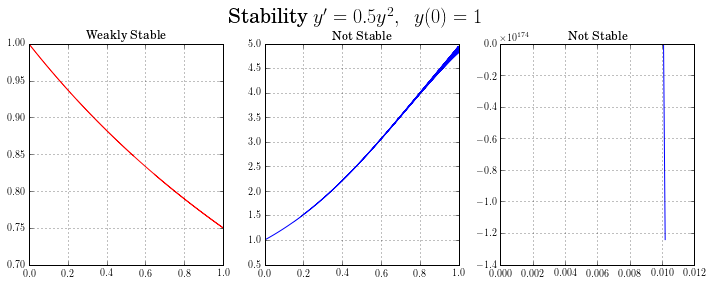
\includegraphics[scale=0.5]{Stability}
\caption{Python output: Left: Weakly stable solution, middle: unstable, right: very unstable }
\label{Stability}
\end{figure}


\newpage
\section{Problem Sheet 4}
\begin{enumerate}
\item
Determine whether the 2-step \addtoindex{Adams-Bashforth} Method is consistent, stable and convergent 
\[ w_{n+1}=w_n+(\frac{3}{2}hf(t_{n},w_{n})-\frac{1}{2}hf(t_{n-1},w_{n-1})),\]

\item
Determine whether the 2-step \addtoindex{Adams-Moulton} Method is consistent, stable and convergent 
\[ w_{n+1}=w_n+\frac{5}{12}hf(t_{n+1},w_{n+1})+\frac{8}{12}hf(t_{n},w_{n})-\frac{1}{12}hf(t_{n-1},w_{n-1}),\]

\item
Determine whether the linear multistep following methods are consistent, stable and convergent 
\begin{enumerate}
\item
\[w_{n+1}=w_{n-1}+\frac{1}{3}h[f(t_{n+1},w_{n+1})+4f(t_n,w_n)+f(t_{n-1},w_{n-1})].\]

\item

\[w_{n+1}=\frac{4}{3}w_{n}-\frac{1}{3}w_{n-1}+\frac{2}{3}h[f(t_{n+1},w_{n+1})]. \]

\end{enumerate}


\end{enumerate}
\newpage



\section{Initial Value Problem Review Questions}
\begin{enumerate}
\item
\begin{enumerate}
\item
Derive the Euler approximation show it has a local truncation error of $O(h)$ of the Ordinary Differential Equation
\[y^{'}(x)=f(x,y) \]
with initial condition
\[y(a)=\alpha. \]
\begin{flushright}
\textbf{[8 marks]}
\end{flushright}
\item 
 Suppose $f$ is a continuous and satisfies a Lipschitz condition with constant
L on $D=\{(t,y)|a\leq t \leq b, -\infty < y < \infty \}$ and that a constant M
exists with the property that 
\[ |y^{''}(t)|\leq M. \]
Let $y(t)$ denote the unique solution of the IVP
\[ y^{'}=f(t,y) \ \ \ a\leq t \leq b \ \ \ y(a)=\alpha \]
and $w_0,w_1,...,w_N$ be the approx generated by the Euler method for some
positive integer N.  Then show for $i=0,1,...,N$
\[ |y(t_i)-w_i| \leq \frac{Mh}{2L}|e^{L(t_i-a)}-1| \]
You may assume the two lemmas:\\
If s and t are positive real numbers $\{a_i\}_{i=0}^{N}$ is a sequence satisfying $a_0 \geq \frac{-t}{s}$ and $a_{i+1} \leq (1+s)a_i +t $
then
\[a_{i+1} \leq e^{(i+1)s}\left(a_0+\frac{t}{s}\right)-\frac{t}{s} \]

For all $ x \geq 0.1$ and any positive m we have \[0\leq (1+x)^m \leq e^{mx}\]
\begin{flushright}
\textbf{[17 marks]}
\end{flushright}
\item
Use Euler's method to estimate the solution of
\[ y^{'}=(1-x)y^2-y; \ \ \ y(0)=1 \]
at x=1, using $h=0.25$.
\begin{flushright}
\textbf{[8 marks]}
\end{flushright}

\end{enumerate}
\item
\begin{enumerate}
\item
Derive the difference equation for the Midpoint Runge Kutta method\\
\[ w_{n+1}=w_n+k_2\]
\[k_1=hf(t_n,w_n)\]
\[k_2=hf(t_n+\frac{1}{2}h,w_n+\frac{1}{2}k_1)\]
for dolving the ordinary differential equation
\[ \frac{dy}{dt}=f(t,y) \]
\[y(t_0)=y_0 \]
by using a formula of the form
\[w_{n+1}=w_n+ak_1+bk_2 \]
where $k_1$ is defined as above,
\[k_2=hf(t_n+\alpha h,w_n+\beta k_1)\]
and $a$, $b$, $\alpha$ and $\beta$ are constants are deteremined. Prove that $a+b=1$ and $b\alpha=b\beta=\frac{1}{2}$ and choose appropriate values to give the Midpoint Runge Kutta method.

\begin{flushright}
\textbf{[18 marks]}
\end{flushright}


\item 
Show that the midpoint Runge Kutta method is stable.
\begin{flushright}
\textbf{[5 marks]}
\end{flushright}

\item
Use the Runge Kutta method to approximate the solutions to the following initial
value problem
\[y^{'}=1+(t-y)^2, \ \ 2\leq t \leq 3, \ \ y(2)=1\]
with $h=0.2$ with the exact solution $y(t)=t +\frac{1}{1-t}$.
\begin{flushright}
\textbf{[10 marks]}
\end{flushright}

\end{enumerate}
\item
\begin{enumerate}
\item
Derive the two step Adams-Bashforth method:
\[ w_{n+1}=w_n+(\frac{3}{2}hf(t_{n},w_{n})-\frac{1}{2}hf(t_{n-1},w_{n-1})),\]
and the local truncation error
\[ \tau_{n+1}(h)=-\frac{5h^2}{12}y^{3}(\mu_n)\]
\begin{flushright}
\textbf{[18 marks]}
\end{flushright}

\item
Apply the two step Adams-Bashforth method to approximate the soluion of the initial value problem:
\[ y'=ty-y, \ \ (0\leq t \leq 2) \ \ \ y(0)=1\].
Using $N=4$ steps, given that $y_1=0.6872$.
\begin{flushright}
\textbf{[15 marks]}
\end{flushright}

\end{enumerate}

\item
\begin{enumerate}
\item
Derive the Adams-Moulton two step method and its truncation error which is of the form
\[w_0=\alpha_0 \ \ \ w_1=\alpha_1 \]
\[w_{n+1}=w_n + \frac{h}{12}[5f(t_{n+1},w_{n+1})+8f(t_{n},w_{n1})-f(t_{n-2},w_{n-2})] \]
and the local truncation error
\[ \tau_{n+1}(h)=-\frac{h^3}{24}y^{4}(\mu_n)\]

\begin{flushright}
\textbf{[23 marks]}
\end{flushright}

\item
Define the terms strongly stable, weakly stable and unstable with respect to the
characteristic equation.
\begin{flushright}
\textbf{[5 marks]}
\end{flushright}
\item
Show that the Adams-Bashforth two step method is  stongly stable.
\begin{flushright}
\textbf{[5 marks]}
\end{flushright}
\end{enumerate}

\item
\begin{enumerate}
\item
Given the initial value problem: 
\[ y'=f(t,y), \ \ \ \  y(t_0)=y_0 \]
and a numerical method which generates a numerical solution $(w_n)_{n=0}^{N}$, explain what it means for the method to be convergent.
\begin{flushright}
\textbf{[5 marks]}
\end{flushright}
\item
Using the 2-step Adams-Bashforth method:
\[ w_{n+1}=w_n+\frac{3}{2}hf(t_n,w_n)-\frac{1}{2}hf(t_{n-1},w_{n-1})\] 
as a predictor, and the 2-step Adams-Moulton method: 
\[w_{n+1}=w_n + \frac{h}{12}[5f(t_{n+1},w_{n+1})+8f(t_{n},w_{n1})-f(t_{n-2},w_{n-2})] \]
as a corrector, apply the 2-step Adams predicitor-corrector method to approximate the solution of the initial value problem
\[y'=ty^3-y, \ \ \ \  (0\leq t \leq 2), \ \ y(0)=1 \]
using N=4 steps, given $y_1=0.5$.
\begin{flushright}
\textbf{[18 marks]}
\end{flushright}

\item
Using the predictor corrector define a bound for the error by controlling the
step size.
\begin{flushright}
\textbf{[10 marks]}
\end{flushright}
\end{enumerate}
\item
\begin{enumerate}
\item
Given the  Midpoint point (Runge- Kutta) method
\[w_0=y_0\]
\[w_{i+1}=w_{i}+hf(x_i+\frac{h}{2},w_i+\frac{h}{2}f(x_i,w_i) ) \]
Assume that the Runge Kutta method satisfies the Lipschitz condition. Then
for the initial value problems
\[ y^{'}=f(x,y)\]
\[ y(x_0)=Y_0 \]
Show that the numerical solution $\{ w_n\}$ satisfies
\[ \max_{a\leq x\leq b}|y(x_n)-w_n| \leq e^{(b-a)L}|y_0-w_0|+\left[\frac{e^{(b-a)L}-1}{L} \right]\tau(h) \]
where
\[\tau(h) = \max_{a\leq x\leq b}|\tau_n(y)|\]
If the consistency condition 
\[ \delta(h) \rightarrow 0 \mbox{ as  } h\rightarrow 0 \]
where
\[\delta(h) = \max_{a \leq x \leq b}|f(x,y)-F(x,y;h;f)| \]
is satisfied then the numerical solution $w_n$ converges to $Y(x_n)$.
\begin{flushright}
\textbf{[18 marks]}
\end{flushright}
\item
Consider the differential equation
\[y^{'}-y+x-2=0, \ \ 0\leq x \leq 1, \ \ y(0)=0.\]
Apply the midpoint method to approximate the solution at $y(0.4)$ using $h=0.2$\\
\begin{flushright}
\textbf{[11 marks]}
\end{flushright}
\item
How would you improve on this result.
\begin{flushright}
\textbf{[4 marks]}
\end{flushright}
\end{enumerate}
\end{enumerate}



\part{Numerical Solutions to Boundary Value Problems}
\chapter{Boundary Value Problems}
\section{Systems of equations}
An m-th order system of equation of first order \addtoindex{Initial Value Problem} can be expressed in the form
\begin{equation}\label{sys eqn}
\begin{array}{cl}
\frac{du_1}{dt}=f_1(t,u_1,...,u_m) \\ 
\frac{du_2}{dt}=f_2(t,u_1,...,u_m) \\ 
.\\
.\\
.\\
\frac{du_m}{dt}=f_m(t,u_1,...,u_m) 
\end{array}
\end{equation}
for $a \leq t \leq b$ with the the initial conditions
\begin{equation}\label{sys con}
\begin{array}{cl}
u_1(a)=\alpha_1\\
u_2(a)=\alpha_2\\
.\\
.\\
.\\
u_m(a)=\alpha_m.
\end{array}
\end{equation}
This can also be written in vector from
\[\mathbf{u^{'}}=\mathbf{f}(t,\mathbf{u}) \]
with initial conditions
\[\mathbf{u(a)=\alpha}.
\]
\begin{definition}
The function $f(t,u_1,...,u_m)$ defined on the set
\[
D=\{(t,u_1,..,u_m)|a\leq t \leq b, -\infty < u_i < \infty, i=1,..,m \}
\]
is said to be a \textbf{\addtoindex{Lipschitz Condition}} on D in the variables $u_1,...,u_m$ if a
constant $L$, the Lipschitz Constant, exists with the property that 
\[ |f(t,u_1,...,u_m)-f(t,z_1,z_2,...,z_m)| \leq L \sum_{j=1}^{m}|u_j-z_j| \]
for all $(t,u_1,...,u_m)$ and $(t,z_1,z_2,...,z_m)$ in $D$.
\end{definition}
\begin{theorem}
Suppose
\[
D=\{(t,u_1,..,u_m)|a\leq t \leq b, -\infty < u_i < \infty, i=1,..,m \}
\]
is continuous on $D$ and satisfy a \addtoindex{Lipschitz Condition}.  The system of 1st order
equations subject th the initial conditions, has a unique solution
$u_1(t),u_2(t),...,u_m(t)$ for $a\leq t \leq b$.
\end{theorem}
\begin{example}
Using Euler method on the system\[
\begin{array}{cl}
u'=u^2-2uv \ \ \ u(0)=1\\
v'=tu+u^2sinv \ \ \ v(0)=-1
\end{array}
\]
for $0\leq t \leq 0.5$ and $h=0.05$
the general Euler difference system of equations is of the form
\[\begin{array}{cl}
\hat{u}_{i+1}=\hat{u}_{i}+hf(t_i,\hat{u}_i,\hat{v}_i) \\
\hat{v}_{i+1}=\hat{v}_{i}+hg(t_i,\hat{u}_i,\hat{v}_i) 
\end{array}
\]
Applied the the \addtoindex{Initial Value Problem}
\[\begin{array}{cl}
\hat{u}_{i+1}=\hat{u}_{i}+0.05(\hat{u}_i^2-2\hat{u}_i\hat{v}_i) \\
\hat{v}_{i+1}=\hat{v}_{i}+0.05(t_i\hat{u}_i+\hat{u}_i^2sin(\hat{v}_i)) 
\end{array}
\]
We know for $i=0$, $\hat{u}_0=1$ and $\hat{v}_0=-1$ from the initial
conditions.\\
For i=0 we have
\[\begin{array}{cl}
\hat{u}_{1}=\hat{u}_{0}+0.05(\hat{u}_0^2-2\hat{u}_0\hat{v}_0) =1.15\\
\hat{v}_{1}=\hat{v}_{0}+0.05(t_0\hat{u}_0+\hat{u}_0^2sin(\hat{v}_0))=-1.042 
\end{array}
\]
and so forth.
\end{example}
\section{Higher order Equations}
\begin{definition}
A general mth order initial value problem
\[y^{(m)}(t)=f(t,y,...,y^{(m-1)}) \ \ a\leq t \leq b \]
with initial conditions
\[y(a)=\alpha_1, y^{'}(a)=\alpha_2,...,y^{(m-1)}(a)=\alpha_m \]
can be converted into a system of equations as in (\ref{sys eqn}) and (\ref{sys con})\\
Let $u_1(t)=y(t), u_1(t)=y^{1}(t),...,u_m(t)=y^{(m-1)}(t) $. This produces
the first order system of equations

\[
\begin{array}{cl}
\frac{du_1}{dt}=\frac{dy}{dt}=u_2\\
\frac{du_2}{dt}=\frac{dy^{'}}{dt}=u_3\\
.\\
.\\
.\\
\frac{du_{m-1}}{dt}=\frac{dy^{(m-2)}}{dt}=u_m\\
\frac{du_m}{dt}=\frac{dy^{(m-1)}}{dt}f_m(t,y,...,y^{(m-1)})=f(t,u_1,...,u_m)
\end{array}
\]
with initial conditions
\[
\begin{array}{cl}
u_{1}(a)=y(a)=\alpha_1\\
u_{2}(a)=y^{'}(a)=\alpha_2\\
.\\
.\\
.\\
u_{m}(a)=y^{(m-1)}(a)=\alpha_m\\
\end{array}
\]
\end{definition}
\begin{example}
\[ y^{''}+3y^{'}+2y=e^t\]
with initial conditions $y(0)=1$ and $y^{'}(0)=2$ can be converted to the system
\[
\begin{array}{cl}
u^{'}=v &u(0)=1\\
v^{'}=e^t-2u-3v &v(0)=2
\end{array}
\]
the difference Euler equation is of the form
\[
\begin{array}{cl}
\hat{u}_{i+1}=\hat{u}_i+hv(t_i,\hat{u}_i,\hat{v}_i)\\
\hat{v}_{i+1}=\hat{v}_i+h(e^{t_i}-2\hat{u}_i-3\hat{v}_i)\\
\end{array}
\]
\end{example}
\section{Boundary Value Problems}
Consider the second order differential equation
\begin{equation}
\label{2nd order ODE}
y^{''}=f(x,y,y^{'})
\end{equation}
defined on an interval $a \leq x \leq b$.  Here $f$ is a function of three variables and $y$ is an unknown.  The general solution to \ref{2nd order ODE}
contains two arbitrary constants so in order to determine it uniquely it is necessary to impose two additional conditions on $y$.  When one of these is given at $x=a$
and the other at $x=b$ the problem is called a 
\addtoindex{boundary value problem} and associated conditions are called boundary conditions.\\
The simplest type of boundary conditions are
\[y(a)=\alpha\]
\[y(b)=\beta \]
for a given numbers $\alpha$ and $\beta$.  However more general conditions such as
\[\lambda_1 y(a)+\lambda_2 y^{'}(a)=\alpha_1 \]
\[\mu_1 y(b)+\mu_2 y^{'}(b)=\alpha_2 \]
for given numbers $\alpha_i, \lambda_i$ and $\mu_i$ (i=1,2) are sometimes imposed.\\
Unlike \addtoindex{Initial Value Problem} whose problems are uniquely solvable \addtoindex{boundary value problem} can have no solution or many.
\begin{example}
The differential equation
\[ y^{''}+y=0\]
\[y_1(x)=y(x) \ \ \ y_2(x)=y^{'}(x)\]
\[y^{'}_1=y_2 \]
\[y^{'}_2=-y_1 \]
It has the general solution 
\[w(x) = C_1sin(x)+C_2 cos(x)\]
where $C_1,C_2$ are constants.\\
The special solution $w(x)=sin(x)$ is the only solution that satisfies 
\[ w(0)=0 \ \ \ w(\frac{\pi}{2})=1 \]
All functions of the form $w(x)=C_1sin(x)$ where $C_1$ is an arbitrary constant,
satisfies
\[ w(0)=0 \ \ \ w(\pi)=0 \]
while there is no solution for the boundary conditions
\[ w(0)=0 \ \ \ w(\pi)=1. \]
 $\diamond$
\end{example}
While we cannot state that all \addtoindex{boundary value problem} are unique we can say a few things.
\section{Some theorems about {boundary value problem}}
Writing the general linear subset \addtoindex{Boundary Value Problem}
\begin{equation}\label{linear BVP}
\begin{array}{l}
y^{''}=p(x)y^{'}+q(x)y+g(x) \ \ \ a < x < b \\
A\left(\begin{array}{c} y(a) \\ y^{'}(a) \end{array} \right)
+
B\left(\begin{array}{c} y(b) \\ y^{'}(b) \end{array} \right)
=
\left(\begin{array}{c} \gamma_1 \\ \gamma_2 \end{array} \right)
\end{array}
\end{equation}
The homogeneous problem is the case in which $g(x)$ and $\gamma_1=\gamma_2=0$.
\begin{theorem}
The non-homogeneous problem (\ref{linear BVP}) has a unique solution $y(x)$ on 
$[a,b]$ for each set of given $\{g(x),\gamma_1,\gamma_2 \}$ if and only if the 
homogeneous problem has only the trivial solutions $y(x)=0$.
\end{theorem}
For conditions under which the homogeneous problem (\ref{linear BVP}) has only
the zero solution we consider the following subset of problem
\begin{equation}\label{linear subset BVP}
\begin{array}{l}
y^{''}=p(x)y^{'}+q(x)y+g(x) \ \ \ a < x < b \\
a_0 y(a)-a_1  y^{'}(a) =\gamma_1 \\
 b_0y(b) +b_1 y^{'}(b) = \gamma_2 \\
\end{array}
\end{equation}
Assume the following conditions
\begin{equation}
\begin{array}{ll}
q(x)>0 & a\leq x \leq b \\
a_0,a_1 \geq 0 & b_0,b_1 \geq 0 \\
\end{array}
\end{equation}
$|a_1|+|a_0|\not= 0, |b_1|+|b_0|\not= 0,|a_0|+|b_0|\not= 0$
Then the homogeneous problem for (\ref{linear subset BVP}) has only the zero solution
therefore the theorem is applicable and the non-homogeneous problem has a unique
solution for each set of data $\{g(x),\gamma_1,\gamma_2 \}$.\\
The theory for a non-linear problem is far more complicated than that of a linear problem. Looking at the class of problems
\begin{equation}\label{non-linear BVP}
\begin{array}{l}
y^{''}=f(x,y,y^{'}) \ \ \ a < x < b \\
a_0 y(a)-a_1  y^{'}(a) =\gamma_1 \\
 b_0y(b) +b_1 y^{'}(b) = \gamma_2 \\
\end{array}
\end{equation}
The function $f$ is assumed to satisfy the following \addtoindex{Lipschitz Condition}
\begin{equation}\label{non-linear Lipschitz BVP}
\begin{array}{l}
|f(x,u_1,v_1)-f(x,u_2,v_2)| \leq K_1|u_1-u_2|\\
|f(x,u_1,v_1)-f(x,u_2,v_2)| \leq K_2|v_1-v_2|\\
\end{array}
\end{equation}
for all points in the region
\[ R=\{(x,u,v)| a\leq x \leq b, -\infty < u,v < \infty \}\]
\begin{theorem}
The problem (\ref{non-linear BVP}) assumes $f(x,u,v)$ is continuous on the region
$R$ and it satisfies the \addtoindex{Lipschitz condition} (\ref{non-linear Lipschitz  BVP}).  In
addition assume that $f$, on $R$, satisfies
\[\frac{\partial f(x,u,v)}{\partial u}> 0 \ \ \ \left|\frac{\partial f(x,u,v)}{\partial v} \right|\leq M \]
for some constant $M>0$ for the boundary conditions of \ref{non-linear BVP} assume
that $|a_1|+|a_0|\not= 0, |b_1|+|b_0|\not= 0,|a_0|+|b_0|\not= 0$.
The \addtoindex{boundary value problem} has a unique solution.
\end{theorem}
\begin{example}
The boundary value problem \addtoindex{boundary value problem}
\[ y^{''} +e^{-xy}+sin(y^{'})=0 \ \ \ 1 < x < 2\]
with $y(1)=y(2)=0$, has
\[ f(x,y,y^{'})=-e^{-xy}-sin(y^{'})\]
Since 
\[\frac{\partial f(x,y,y^{'})}{\partial y} =xe^{xy} >0 \]
and
\[\left|\frac{\partial f(x,y,y^{'})}{\partial y^{'}}\right| =|-cos(y^{'}) \leq1 \]
this problem has a unique solution.
$\diamond$
\end{example}
\section{Shooting Methods}
The principal of the shooting method is to change our original boundary value problem \addtoindex{boundary value problem} into 2 \addtoindex{Initial Value Problem}.
\subsection{Linear Shooting method}
Looking at problem class (\ref{linear subset BVP}).  We break this down into two
\addtoindex{Initial Value Problem}.
\begin{equation}
\begin{split}
 y^{''}_1=p(x)y^{'}_1+q(x)y_1+r(x), \ \    y_1(a)=\alpha, \ \ y^{'}_1(a)=0\\
y^{''}_2=p(x)y^{'}_2+q(x)y_2, \ \ y_2(a)=0, \ \ y^{'}_2(a)=1
\end{split}
\end{equation}


combining these results together to get the unique solution 
\begin{equation}
y(x)=y_1(x)+\frac{\beta-y_1(b)}{y_2(b)}y_2(x)
\end{equation}
provided that $y_2(b)\not=0$.
\begin{example}
\[ y^{''}=2y^{'}+3y-6 \]
with boundary conditions
\[y(0) = 3 \]
\[y(1) = e^3+2 \]
The exact solution is 
\[y=e^{3x}+2 \]
breaking this \addtoindex{boundary value problem} into two \addtoindex{Initial Value Problem}'s
\begin{equation}
\label{Shoot A}
y^{''}_1 =2y^{'}_1+3y_{1}-6 \ \ \ \ y_1(a)=3, \ \ \ y^{'}_1(a)=0\end{equation}
\begin{equation}
\label{Shoot B}
y^{''}_2 =2y^{'}_2+3y_{2} \ \ \ \ y_2(a)=0, \ \ \ y^{'}_2(a)=1\end{equation}
Discretising (\ref{Shoot A})
\[ y_1=u_1 \ \ \ y_1^{'}=u_2\]
\[u_1^{'}=u_2 \ \  u_1(a)=3\]
\[u_2^{'}=2u_2+3u_1-6 \ \ \ u_2(a)=0\]
using the Euler method we have the two difference equations
\[u_{1 i+1}=u_{1 i} + h u_{2 i}\]
\[u_{2 i+1}=u_{2 i} + h (2u_{2 i}+3u_{1 i} -6)\]
Discretising (\ref{Shoot B})
\[ y_2=w_1 \ \ \ \  y_2^{'}=w_2\]
\[w_1^{'}=w_2 \ \ \  w_1(a)=0\]
\[w_2^{'}=2w_2+3w_1 \ \ \ w_2(a)=1\]
using the Euler method we have the two difference equations
\[w_{1 i+1}=w_{1 i} + h w_{2 i}\]
\[w_{2 i+1}=w_{2 i} + h (2w_{2 i}+3w_{1 i})\]
combining all these to get our solution
\[y_i=u_{1 i} + \frac{\beta-u_{1}(b)}{w_1(b)}w_{1 i}\]
It can be said 
\[ |y_i - y(x_i)| \leq K h^n\left|1+\frac{w_{1 i}}{u_{1 i}}\right| \]
$O(h^n)$ is the order of the method.
\end{example}


\begin{figure}[H]
\centering
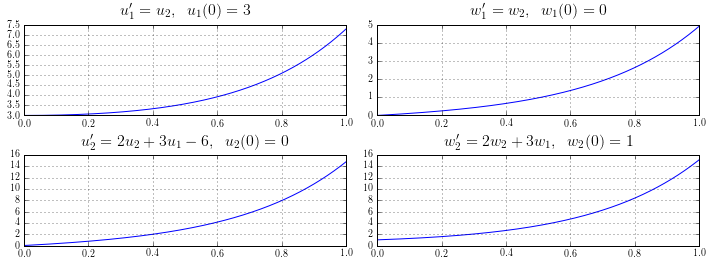
\includegraphics[scale=0.5]{Shooting_linear_method_all}
\caption{Python output: Shooting Method}
\label{Shooting_method}
\end{figure}

\begin{figure}[H]
\centering
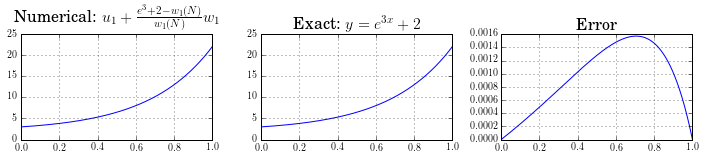
\includegraphics[scale=0.5]{Shooting_linear_method_Num_analyt_error}
\caption{Python output: Shooting Method error}
\label{Shooting_method_error}
\end{figure}

\subsection{The Shooting method for non-linear equations}
\begin{example}
\[y^{''}=-2yy^{'} \ \ \ y(0)=0 \ \ y(1)=1\]
The corresponding initial value problem is 
\begin{equation}\label{shoot non-lin}
y^{''}=-2yy^{'} \ \ \ y(0)=0 \ \  y^{'}(0)=\lambda \end{equation}
Which reduces to the first order system, letting $y_1=y$ and $y_2=y^{'}$. 
\[ y^{'}_1=y_2 \ \ \ y_1(0)=0 \]
\[y^{'}_2=-2y_1y_2 \ \ \ y^{'}_2(0)=\lambda \]
Taking $\lambda =1$ and $\lambda=2$ as the first and second guess of $y^{'}(0)$.
(\ref{shoot non-lin}) depends on two variable $x$ and $\lambda$.
$\diamond$
\end{example}
\textbf{How to choose $\lambda$?}\\
Our goal is to choose $\lambda$ such that,
\[F(\lambda)=y(b,\lambda)-\beta=0. \]
We use \addtoindex{Newton's method} to generate the sequence $\lambda_k$ with only the initial approx $\lambda_0$.
The iteration has the form
\[\lambda_k=\lambda_{k-1}-\frac{y(b,\lambda_{k-1})-\beta}{\frac{dy}{d \lambda}(b,\lambda_{k-1})}\]
and requires knowledge of $\frac{dy}{d \lambda}(b,\lambda_{k-1})$.  This present
a difficulty since an explicit representation for $y(b,\lambda)$ is unknown we only know
$y(b,\lambda_0),$ $y(b,\lambda_1),...,y(b,\lambda_{k-1})$.\\
Rewriting our \addtoindex{Initial Value Problem} we have it so that it depends on both $x$ and $\lambda$.
\[ y^{''}(x,\lambda)=f(x,y(x,\lambda),y^{'}(x,\lambda)), \ \ a\leq x \leq b,\]
with the initial conditions,
\[y(a,\lambda)=\alpha \ \ y^{'}(a,\lambda)=\lambda, \]
differentiating with respect to $\lambda$ and let $z(x,\lambda)$ denote $\frac{\partial y}{\partial\lambda}(x,\lambda)$ we have,
\[
\frac{\partial }{\partial \lambda}(y^{''}) = \frac{\partial f}{\partial \lambda}=\frac{\partial f}{\partial y}
\frac{\partial y}{\partial \lambda}+
\frac{\partial f}{\partial y^{'}}
\frac{\partial y^{'}}{\partial \lambda}.
\]
Now 
\[\frac{\partial y^{'} }{\partial \lambda}=\frac{\partial}{\partial \lambda}\frac{\partial y}{\partial x}
=\frac{\partial }{\partial x}\left( \frac{\partial y}{\partial \lambda}\right)
=\frac{\partial z}{\partial x}=z^{'},\]
we have
\[ z^{''}(x,\lambda)=\frac{\partial f}{\partial y}z(x,\lambda)+\frac{\partial f}{\partial y^{'}}z^{'}(x,\lambda) \]
for $a \leq x \leq b$ and the initial conditions,
\[z(a,\lambda)=0, \ \ \ z^{'}(a,\lambda)=1 \]
Now we have 
\[\lambda_k=\lambda_{k-1}-\frac{y(b,\lambda_{k-1})-\beta}{z(b,\lambda_{k-1})}\]
We can solve the original non-linear subset \addtoindex{Boundary Value Problem} by solving the two \addtoindex{Initial Value Problem}'s.
\begin{example}(cont.)\\
\[\frac{\partial f}{\partial y}=-2y^{'} \ \ \ \frac{\partial f}{\partial y^{'}}=-2y\]
We now have the two \addtoindex{Initial Value Problem}'s
\[y^{''}=-2yy^{'} \ \ \ y(0)=0 \ \ y^{'}(0)=\lambda \]
\begin{eqnarray*}
z^{''}&=&\frac{\partial f}{\partial y}z(x,\lambda)+\frac{\partial f}{\partial y^{'}}z^{'}(x,\lambda)\\
&=&-2y^{'}z-2yz^{'} \ \ z(0)=0 \ \ z^{'}(0)=1 \end{eqnarray*}
Discretising we let $y_1=y$, $y_2=y^{'}$, $y_3=z$ and $y_4=z^{'}$.
\begin{eqnarray*}
y_1^{'}=y_2 &\ \ : \ \  &y_1(0)=0 \\
y_2^{'}=-2y_1y_2 &\ \ : \ \  &y_2(0)=\lambda_k \\
z_1^{'}=z_2 &\ \ : \ \  &z_1(0)=0 \\
z_2^{'}=-2z_1y_2-2y_1z_2 &\ \ : \ \  &y_2(0)=1 
\end{eqnarray*}
with
\[\lambda_k=\lambda_{k-1}-\frac{y_1(b)-\beta}{y_3(b)} \]
Then solve using a one step method.
$\diamond$
\end{example}


\begin{figure}[H]
\centering
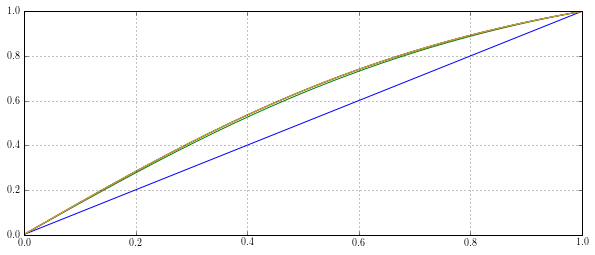
\includegraphics[scale=0.5]{Shooting_nonlinear_method_all}
\caption{Python output: Nonlinear Shooting Method}
\label{Shooting_method_nl}
\end{figure}

\begin{figure}[H]
\centering
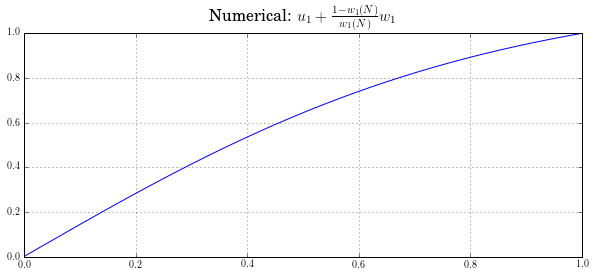
\includegraphics[scale=0.5]{Shooting_nonlinear_method_solnl}
\caption{Python output: Nonlinear Shooting Method result}
\label{Shooting_method_error}
\end{figure}

\begin{figure}[H]
\centering
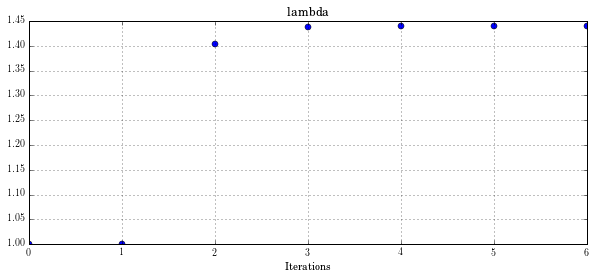
\includegraphics[scale=0.5]{Shooting_nonlinear_method_lambda}
\caption{Python output: Nonlinear Shooting Method $\lambda$}
\label{Shooting_method_error}
\end{figure}



\section{Finite Difference method}
Each finite difference operator can be derived from Taylor expansion.\\
Once again looking at a linear second order differential equation
\[y^{''}=p(x)y^{'}+q(x)y+r(x) \]
on $[a,b]$ subject to boundary conditions
\[ y(a)=\alpha \ \ \ y(b) =\beta \]
As with all cases we divide the area into even spaced mesh points
\[x_0=a, \ \ x_N=b \ \ \ x_i=x_0+ih \ \ h=\frac{b-a}{N} \]
We now replace the derivatives $y^{'}(x)$ and $y^{''}(x)$ with the centered difference approximations
\[y^{'}(x)=\frac{1}{2h}(y(x_{i+1})-y(x_{i-1}))-\frac{h^2}{12}y^{3}(\xi_i) \]
\[y^{''}(x)=\frac{1}{h^2}(y(x_{i+1})-2y(x_i)+y(x_{i-1}))-\frac{h^2}{6}y^{4}(\mu_i) \]
for some $x_{i-1} \leq \xi_i \mu_i \leq x_{i+1}$ for i=1,...,N-1.\\
We now have the equation
\[
\frac{1}{h^2}(y(x_{i+1})-2y(x_i)+y(x_{i-1}))=p(x_i)\frac{1}{2h}(y(x_{i+1})-y(x_{i-1}))+q(x_i)y(x_i)+r(x_i)\]
This is rearranged such that we have all the unknown together,
\[\left(1+\frac{hp(x_i)}{2} \right)y(x_{i-1})-(2+h^2q(x_i))y(x_i)+\left(1-\frac{hp(x_i)}{2} \right)y(x_{i+1})=h^2r(x_i) \]
for $i=1,..,N-1$.\\
Since the values of $p(x_i),q(x_i)$ and $r(x_i)$ are known it represents a linear
algebraic equation involving $y(x_{i-1}), y(x_{i}),y(x_{i+1})$.\\
This produces a system of $N-1$ linear equations with $N-1$ unknowns $y(x_1),...,y(x_{N-1})$.\\
The first equation corresponding to $i=1$ simplifies to 
\[-(2+h^2q(x_1))y(x_1)+\left(1-\frac{hp(x_1)}{2} \right)y(x_{2})=h^2r(x_1)-\left(1+\frac{hp(x_1)}{2} \right)\alpha \]
because of the boundary condition $y(a)=\alpha$, and for $i=N-1$
\[ \left(1+\frac{hp(x_{N-1})}{2} \right)y(x_{N-2}) -(2+h^2q(x_{N-1}))y(x_{N-1})=h^2r(x_{N-1})-\left(1-\frac{hp(x_{N-1})}{2} \right)\beta \]
because $y(b)=\beta$.\\
The values of $y_i, \ (i=1,...,N-1)$ can therefore be found by solving the tridiagonal system
\[A\mathbf{y}=\mathbf{b} \]
where
\[
A =\]
\[\begin{bmatrix}
-(2+h^2q(x_1)) & \left(1-\frac{hp(x_1)}{2}\right) & 0 &.&0 \\
 \left(1+\frac{hp(x_2)}{2}\right)&-(2+h^2q(x_2)) & \left(1-\frac{hp(x_2)}{2}\right) & 0 &.  \\
0&.&.&0&0\\
.&.&.&.&.\\
.&.&.&.&.\\
 .&0&\left(1+\frac{hp(x_{N-2})}{2}\right)&-(2+h^2q(x_{N-2})) & \left(1-\frac{hp(x_{N-2})}{2}\right) \\
 .&0&0&\left(1+\frac{hp(x_{N-1})}{2}\right)&-(2+h^2q(x_{N-1})) 
\end{bmatrix}
\]
\[
y =\left( \begin{array}{c}
y_1 \\
y_2 \\
. \\
. \\
y_{N-2} \\
y_{N-1} 
\end{array}\right)
b =\left( \begin{array}{c}
h^2r_1-\left( 1+\frac{hp_1}{2}\right)\alpha \\
h^2r_2 \\
. \\
. \\
h^2r_{N-2} \\
h^2r_{N-1}-\left( 1-\frac{hp_1}{2}\right)\beta
\end{array}\right)
\]
\begin{example}
Looking at the simple case
\[\frac{d^2y}{dx^2}=4y, \ \ y(0)=1.1752, \ \ y(1)=10.0179. \]
Our difference equation is
\[
\frac{1}{h^2}(y(x_{i+1})-2y(x_i)+y(x_{i-1}))=4y(x_i) \ \ \ i=1,..,N-1 \]
dividing $[0,1]$ into 4 subintervals we have $h=\frac{1-0}{4}$
\[x_i=x_0+ih=0+i(0.25)\]
In this simple example $q(x)=4$, $p(x)=0$ and $r(x)=0$. Rearranging the
equation we have
\[ \frac{1}{h^2} (y(x_{i+1})) -\left(\frac{2}{h^2}+4\right)y(x_i) +\frac{1}{h^2} (y(x_{i-1}))=0\]
multiplying across by $h^2$
\[  y(x_{i+1}) -(2+4h^2)y(x_i) + (y(x_{i-1}))=0\]
with the boundary conditions $y(x_0)=1.1752$ and $y(x_4)=10.0179$.
Our equations are of the form
\begin{eqnarray*}
y(x_2)-2.25y(x_1)=-1.1752\\
y(x_3)-2.25y(x_2)+y(x_1)=0\\
-2.25y(x_3)+y(x_2)=-10.0179
\end{eqnarray*}
Putting this into matrix form 
\[\left(\begin{array}{ccc} -2.25&1&0\\
1&-2.25&1\\
0&1&-2.25
\end{array}\right)
\left(\begin{array}{c} y_1\\
y_2\\
y_3
\end{array}\right)
=
\left(\begin{array}{c}-1.1752\\
0\\
-10.0179 \end{array}\right)
\]
\begin{center}
\begin{tabular}{l|l|c}
$x$ & $y$ & Exact $sinh(2x+1)$\\
\hline
0 & 1.1752&1.1752\\
0.25 & 2.1467 & 2.1293\\
0.5 & 3.6549& 3.6269\\
0.75 & 6.0768& 6.0502\\
1.0& 10.0179& 10.0179\\
\end{tabular}
\end{center}
\end{example}$\diamond$
\begin{example}
Looking at a more involved \addtoindex{boundary value problem}
\[y^{''}=xy^{'}-3y+e^x \ \ \ y(0)=1 \ \ y(1)=2 \]
Let N=5 then $h=\frac{1-0}{5}=0.2$. The difference equation is of the form
\[
\frac{1}{h^2}(y(x_{i+1})-2y(x_i)+y(x_{i-1}))=x_i\frac{1}{2h}(y(x_{i+1})-y(x_{i-1}))-3y(x_i)+e^{x_i}\]
Re arranging and putting $h=0.2$
\[(1+\frac{0.2(x_i)}{2})y(x_{i-1})-(1.88)y(x_i)+(1-\frac{0.2(x_i)}{2})y(x_{i+1})=0.04e^{x_i} \]
In matrix form this is
\[\left(\begin{array}{cccc} -1.88&0.98&0&0\\
1.04&-1.88&0.96&0\\
0&1.06&-1.88&0.94\\
0&0&1.08&-1.88
\end{array}\right)
\left(\begin{array}{c} y_1\\
y_2\\
y_3\\
y_4
\end{array}\right)
=
\left(\begin{array}{c}
0.04e^{0.2}-1.02\\
0.04e^{0.4}\\
0.04e^{0.6}\\
0.04e^{0.8}-1.84 
\end{array}\right)
\]
$y_1=1.4651$, $y_2=1.8196$, $y_3=2.0283$ and $y_4=2.1023$.
\end{example}
\section*{Solving a tri-diagonal system}
To solve a tri-diagonal system we can use the method discussed in the approximation theory.

\newpage
\section{Problem Sheet 6 - Boundary Value Problems}
\begin{enumerate}
\item
	Consider the boundary value problem 
	\[y''=3xy'-4y+x^2, \ \ 1\leq x \leq 2, \ \ y(1)=2,\ \ \ y(2)=-1. \]
	Apply the linear shooting method to transform this equation into two second order initial value problems
	and approximate the solution using the Euler method with stepsize $h=\frac{1}{3}.$
\end{enumerate}
\part{Numerical Solutions to Partial Differential Equations}

\chapter{Partial Differential Equations}
\section{Introduction}
Partial Differential Equations (\addtoindex{PDE}), occur frequently in maths, natural science
and engineering.\\
\addtoindex{PDE}'s are problems involving rates of change of functions of several variables.\\
The following involve 2 independent variables:
\begin{eqnarray*}
-\nabla^2u=-\frac{\partial^2u}{\partial x^2}-\frac{\partial^2u}{\partial y^2}=f(x,y)&\mbox{Poisson Eqn}\\
\frac{\partial u}{\partial t}+v\frac{\partial u}{\partial x}=0&\mbox{Advection Eqn}\\
\frac{\partial u}{\partial t}-D\frac{\partial^2 u}{\partial x^2}=0&\mbox{Heat Eqn}\\
\frac{\partial^2 u}{\partial t^2}-c^2\frac{\partial^2 u}{\partial x^2}=0&\mbox{Wave Equation}
\end{eqnarray*}
Here $v,D,c$ are real positive constants.  In these cases $x,y$ are the space
coordinates and $t,x$ are often viewed as time and space coordinates, respectively.\\
These are only examples and do not cover all cases.  In real occurrences \addtoindex{PDE}'s
usually have 3 or 4 variables.\\
\section{PDE Classification}
\addtoindex{PDE}'s in two independent variables x and y have the form
\[ \Phi\left(x,y,u,\frac{\partial u}{\partial x},\frac{\partial u}{\partial y},\frac{\partial^2 u}{\partial x^2},...\right) = 0 \]
where the symbol $\Phi$ stands for some functional relationship.\\
As we saw with BVP this is too general a case so we must define new classes of the
general \addtoindex{PDE}.
\begin{definition}
The order of a \addtoindex{PDE} is the order of the highest derivative that appears.\\
ie Poisson is 2nd order, Advection eqn is 1st order. $\circ$
\end{definition}
Most of the mathematical theory of \addtoindex{PDE}'s concerns linear equations of first or second order.\\
After order and linearity (linear or non-linear), the most important classification
scheme for \addtoindex{PDE}'s involves geometry.\\
Introducing the ideas with an example:\\
\begin{example}
\begin{equation}\label{ex}
\alpha(t,x)\frac{\partial u}{\partial t}+\beta\frac{\partial u}{\partial x}=\gamma(t,x)\end{equation}
A solution $u(t,x)$ to this \addtoindex{PDE} defines a surface $\{t,x,u(t,x)\}$ lying over some region of the $(t,x)$-plane.\\
Consider any smooth path in the $(t,x)$-plane lying below the solution $\{t,x,u(t,x)\}$.\\  Such a path has a parameterization $(t(s),x(s))$ where the parameter
s measures progress along the path.\\
What is the rate of change $\frac{d u}{d s}$ of the solution as we travel along the path $(t(s),x(s))$.\\
The chain rule provides the answer
\begin{equation}\label{chain}\frac{d t}{d s}\frac{\partial u}{\partial t}+
\frac{d x}{d s}\frac{\partial u}{\partial x}
=\frac{d u}{d s}\end{equation}
Equation (\ref{chain}) holds for an arbitrary smooth path in the $(t,x)$-plane.  
Restricting attention to a specific family of paths leads to a useful observation:
When
\begin{equation}\frac{dt}{ds}=\alpha(t,x) \mbox{  and  } \frac{dx}{ds}=\beta(t,x)
\end{equation}
the simultaneous validity of (\ref{ex}) and (\ref{chain}) requires that
\begin{equation}\label{gamma}
\frac{du}{ds}=\gamma(t,x).
\end{equation}
Equation (\ref{gamma}) defines a family of curves $(t(s),x(s))$ called characteristic curves in the plane $(t,x)$.\\
Equation (\ref{gamma}) is an ode called the characteristic equation that the solution must satisfy along only the characteristic curve.\\
Thus the original \addtoindex{PDE} collapses to an ODE along the characteristic curves. Characteristic 
curves are paths along which information about the solution to the \addtoindex{PDE} propagates
from points where the initial value or boundary values are known.
$\diamond$\end{example}
Consider a second order \addtoindex{PDE} having the form
\begin{equation}
\alpha(x,y)\frac{\partial^2u}{\partial x^2}+\beta(x,y)\frac{\partial^2 u}{\partial x\partial y}+\gamma(x,y)\frac{\partial^2u}{\partial y^2} = \Psi(x,y,u,\frac{\partial u}{\partial x},\frac{\partial u }{\partial y})
\end{equation}
Along an arbitrary smooth curve $(x(s),y(s))$ in the $(x,y)$-plane, the gradient
$\left( \frac{\partial u}{\partial x}, \frac{\partial u}{\partial y}\right)$ of the solution varies according to the chain rule:
\[ \frac{dx}{ds}\frac{\partial^2u}{\partial y\partial x}+\frac{dy}{ds}\frac{\partial^2 u}{\partial y\partial x}=\frac{d}{ds}\left(\frac{\partial u}{\partial x}\right)\]
\[ \frac{dx}{ds}\frac{\partial^2u}{\partial x \partial y}+\frac{dy}{ds}\frac{\partial^2u}{\partial y^2}=\frac{d}{ds}\left(\frac{\partial u}{\partial y}\right)\]
if the solution $u(x,y)$ is continuously differentiable then these relationships
together with the original \addtoindex{PDE} yield the following system:
\begin{equation}
\label{matrix char} 
\left(\begin{array}{ccc}
\alpha & \beta & \gamma \\
\frac{dx}{ds}&\frac{dy}{ds}&0\\
0&\frac{dx}{ds}&\frac{dy}{ds}\\
\end{array}\right)
\left(\begin{array}{c}
\frac{\partial^2u}{\partial x^2}\\
\frac{\partial^2u}{\partial x\partial y}\\
\frac{\partial^2u}{\partial y^2}\\
\end{array}\right)
=
\left(\begin{array}{c}
\Psi\\
\frac{d}{ds}\left(\frac{\partial u}{\partial x}\right)\\
\frac{d}{ds}\left(\frac{\partial u}{\partial y}\right)\\
\end{array}\right)
\end{equation} 
By analogy with the first order case we determine the characteristic curves bu where the \addtoindex{PDE} is redundant  with the chain rule.  This occurs when the determinant
of the matrix in (\ref{matrix char}) vanishes that is when
\[
\alpha\left( \frac{dy}{ds}\right)^2
-
\beta\left( \frac{dy}{ds}\right)\left( \frac{dx}{ds}\right)
+
\gamma\left( \frac{dx}{ds}\right)^2=0
\]
eliminating the parameter $s$ reduces this equation to the equivalent condition
\[
\alpha\left( \frac{dy}{dx}\right)^2
-
\beta\left( \frac{dy}{dx}\right)
+
\gamma
=0
\]
Formally solving this quadratic for $\frac{dy}{dx}$, we find
\[\frac{dy}{dx}=\frac{\beta\pm\sqrt{\beta^2-4\alpha\gamma}}{2\alpha}\]
This pair of ODE's determine the characteristic curves.  From this equation we
divide into 3 classes each defined with respect to $\beta^2-4\alpha\gamma$.
\begin{enumerate}
\item
\textbf{HYPERBOLIC}\\
$\beta^2-4\alpha\gamma>0$
This gives two families of real characteristic curves.
\item
\textbf{PARABOLIC}\\
$\beta^2-4\alpha\gamma=0$
This gives exactly one family of real characteristic curves.
\item
\textbf{ELLIPTIC}\\
$\beta^2-4\alpha\gamma<0$
This gives no real characteristic equations.
\end{enumerate}
\begin{example}
\underline{The wave equation}
\[c^2\frac{\partial^2u}{\partial x^2}-\frac{\partial^2u}{\partial t^2}=0\]
now equating this with our formula for the characteristics we have
\[\frac{dt}{dx}=\frac{0\pm\sqrt{0+4c^2}}{2}=\pm c\]
this implies that the characteristics are $x+ct=const$ and $x-ct=const$.
This means that the effects travel along the characteristics.\\
\underline{Laplace equation}
\[\frac{\partial^2 u}{\partial x^2} + \frac{\partial^2u}{\partial y^2} =0\]
from this we have $-4(1)(1)< 0$ which implies it is elliptic.\\
This means that information at one point affects all other points.\\
\underline{\addtoindex{Heat equation}}
\[\frac{\partial^2u}{\partial x^2}-\frac{\partial u}{\partial t}=0\]
from this we have $\beta^2-4\alpha\gamma=0$ this implies that the equation is
parabolic thus we have
\[ \frac{\partial t}{\partial x}=0\]
$\diamond$\\
\end{example} 
We can also state that hyperbolic and parabolic are Boundary value problems
and initial value problems.  While, elliptic problems are boundary value problems.

\section{Difference Operators}
Through out this chapter we will use $U$ to denote the exact solution and 
$w$ to denote the numerical (approximate) solution.\\
1-D difference operators
\begin{eqnarray*}
D^{+}U_{i}=\frac{U_{i+1}-U_{i}}{h_{i+1}} \ \ \ \mbox{ Forward} \\
D^{-}U_{i}=\frac{U_{i}-U_{i-1}}{h_i} \ \ \ \mbox{ Backward} \\
D^{0}U_{i}=\frac{U_{i+1}-U_{i-1}}{x_{i+1}-x_{i-1}} \ \ \ \mbox{ Centered} \\
\end{eqnarray*}
For 2-D Differences Schemes is similar when dealing with the x-direction we hold
the y-direction constant and then dealing with the y-direction hold the x-direction
constant.
\begin{eqnarray*}
D^{+}_xU_{ij}=\frac{U_{i+1j}-U_{ij}}{x_{i+1}-x_{i}} \ \ \ \mbox{ Forward in the x-direction} \\
D^{+}_yU_{ij}=\frac{U_{ij+1}-U_{ij}}{y_{i+1-y_{i}}} \ \ \ \mbox{ Forward in the y-direction} \\
D^{-}_xU_{ij}=\frac{U_{ij}-U_{i-1j}}{x_i-x_{i-1}} \ \ \ \mbox{ Backward in the x direction} \\
D^{-}_yU_{ij}=\frac{U_{ij}-U_{ij-1}}{y_i-y_{i-1}} \ \ \ \mbox{ Backward in the y direction} \\
D^{0}_xU_{ij}=\frac{U_{i+1j}-U_{i-1j}}{x_{i+1}-x_{i-1}} \ \ \ \mbox{ Centered in the x direction} \\
D^{0}_yU_{ij}=\frac{U_{ij+1}-U_{ij-1}}{y_{i+1}-y_{i-1}} \ \ \ \mbox{ Centered in the y direction} 
\end{eqnarray*}
Second derivatives
\begin{eqnarray*}
\delta_x^{2}U_{ij}=\frac{2}{x_{i+1}-x_{i-1}}\left(\frac{U_{i+1j}-U_{ij}}{x_{i+1}-x_{i}}-\frac{U_{ij}-U_{i-1j}}{x_{i}-x_{i-1}}\right) \ \ \ \mbox{ Centered in $x$ direction} \\
\delta_y^{2}U_{ij}=\frac{2}{y_{i+1}-y_{i-1}}\left(\frac{U_{ij+1}-U_{ij}}{y_{i+1}-y_{i}}-\frac{U_{ij}-U_{ij-1}}{y_{i}-y_{i-1}}\right) \ \ \ \mbox{ Centered in y direction} \\
\end{eqnarray*}

\chapter{Parabolic equations}
We will look at the \addtoindex{Heat equation} as our sample parabolic equation.
\[ \frac{\partial U}{\partial T}=K\frac{\partial^2U }{\partial X^2} \mbox{ on } \Omega \]
and 
\[ U=g(x,y) \mbox{ on the boundary } \delta\Omega \]
this can be transformed without loss of generality by a non-dimensional transformation to

\begin{equation}\label{heat} \frac{\partial U}{\partial t}=\frac{\partial^2U }{\partial x^2}\end{equation}

\section{An explicit method for the heat eqn}
The explicit Forwards Time Centered Space (FTCS) equation difference equation of the differential equation (\ref{heat}) is
\begin{equation}
\frac{w_{ij+1}-w_{ij}}{t_{j+1}-t_{j}}=\frac{w_{i+1j}-2w_{ij}+w_{i-1j}}{h^2},
\end{equation}

\begin{equation*}
\frac{w_{ij+1}-w_{ij}}{k}=\frac{w_{i+1j}-2w_{ij}+w_{i-1j}}{h^2}
\end{equation*}
when approaching this we have divided up the area into
two uniform meshes one in the x direction and the other in the t-direction.
We define $t_j=jk$ where k is the step size in the time direction.\\
We define $x_i=ih$ where h is the step size in the space direction.\\
$w_{ij}$ denotes the numerical approximation of $U$ at $(x_i,t_j)$.\\
Rearranging the equation we get
\begin{equation}\label{disc heat}
w_{ij+1}=rw_{i-1j}+(1-2r)w_{ij}+rw_{i+1j}
\end{equation}
where $r=\frac{k}{h^2}$.\\
This gives the formula for the unknown term $w_{ij+1}$ at the $(ij+1)$ mesh points
in terms of terms along the jth time row.\\
Hence we can calculate the unknown pivotal values of $w$ along the first row $t=k$ or $j=1$ in terms of the known boundary conditions.\\
This can be written in matrix from 
\[ \mathbf{w}_{j+1}=A\mathbf{w}_{j} +\mathbf{b}_{j} \]
for which $A$ is
\[
\left(\begin{array}{ccccccc}
1-2r&r&0&.&.&.&.\\
r&1-2r&r&0&.&.&.\\
0&r&1-2r&r&0&.&.\\
.&.&.&.&.&.&.\\
.&.&.&.&r&1-2r&r\\
.&.&.&.&.&r&1-2r\\
\end{array}\right)
\]
where $r=\frac{k}{h_x^2}>0$, $\mathbf{w}_j$ is 
\[
\left(\begin{array}{c}
w_{1j}\\
w_{2j}\\
.\\
w_{N-2j}\\
w_{N-1j}\\

\end{array}\right)
\]
and $\mathbf{b}_j$ is 
\[
\left(\begin{array}{c}
rw_{0j}\\
0\\
.\\
0\\
rw_{Nj}\\
\end{array}\right).
\]
It is assumed that the boundary values $w_{0j}$ and $w_{Nj}$ are known for $j=1,2,...$, and $w_{i0}$ is the initial condition.

\subsection{Example explicit method for the Heat Equation} 
In this case we look at a rod of unit length with each end in ice.\\
The rod is heat insulated along its length so that temperature changes occur through
heat conduction along its length and heat transfer at its ends, where w denotes
temperature.\\

\textbf{Simple case}\\
Given that the ends of the rod are kept in contact with ice and the initial temperature
distribution is non dimensional form is
\begin{enumerate}
\item $U=2x$ for $0\leq x \leq \frac{1}{2}$, 
\item $U=2(1-x)$ for $\frac{1}{2}\leq x \leq 1$. 
\end{enumerate}
In other words we are seeking a numerical solution of
\[\frac{\partial U}{\partial t}=\frac{\partial^2U }{\partial x^2}\]
which satisfies
\begin{enumerate}
\item $U=0$ at $x=0$ for all $t>0$ (the boundary condition)
\item $U=2x$ for $0\leq x \leq \frac{1}{2}$ for t=0
$U=2(1-x)$ for $\frac{1}{2}\leq x \leq 1$ for t=0 (the initial condition)
\end{enumerate}
The problem is symmetric with respect to $x=0.5$ so we need the solution only for $0\leq x \leq \frac{1}{2}$
\begin{example}
\subsubsection{Explicit FTCS method for the Heat Equation with $r=\frac{1}{10}$}
Let $h=\frac{1}{5}$ and $k=\frac{1}{250}$ so that $r=\frac{k}{h^2}=\frac{1}{10}$
difference equation (\ref{disc heat}) becomes
\[
w_{ij+1}=\frac{1}{10}(w_{i-1j}+8w_{ij}+w_{i+1j}).
\]
This can be written in matrix form 
\[
\left(\begin{array}{c}
w_{1j+1}\\
w_{2j+1}\\
w_{3j+1}\\
w_{4j+1}
\end{array}\right)
=
\left(\begin{array}{cccc}
0.8&0.1&0&0\\
0.1&0.8&0.1&0\\
0&0.1&0.8&0.1\\
0&0&0.1&0.8
\end{array}\right)
\left(\begin{array}{c}
w_{1j}\\
w_{2j}\\
w_{3j}\\
w_{4j}
\end{array}\right)+0.1\left(\begin{array}{c}
w_{0j}\\
0\\
0\\
w_{5j}
\end{array}\right).
\]
Figure \ref{Matrix_FTCS_1_10} shows a graphical representation of the matrix.
\begin{figure}[H]
  \caption{Graphical representation of the matrix A for $r=\frac{1}{10}$. }
  \centering
    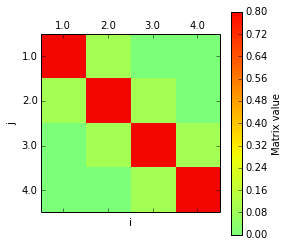
\includegraphics[width=0.5\textwidth]{HeatEquationFigures/r_equals_one_tenth/Matrix}
    \label{Matrix_FTCS_1_10}
\end{figure}
To solve for $w_{21}$ we have
\[w_{21}=\frac{1}{10}(w_{10}+8w_{20}+w_{30})=\frac{1}{10}(0.4+8\times 0.8+0.8)=0.76. \]
Table \ref{Table_FTCS_1_10} shows the initial condition and one time step for the Heat Equation.
\begin{center}
 \begin{table}[H]
 \caption{The explicit numerical solution $w$ of the Heat Equation for $r=\frac{1}{10}$ for $1$ time step.}
 \label{Table_FTCS_1_10}
 \centering
\begin{tabular}{l|cccccc}
j/x&0&0.2&0.4&0.6&0.8&1.0\\ \hline
0&0&0.4&0.8&0.8&0.4&0.0\\
$\frac{1}{250}$&0&0.4&0.76&0.76&0.4&0.0
\end{tabular}
\end{table}
\end{center}

Figure \ref{Plot_FTCS_1_10} shows the explicit numerical solution $w$ of the Heat Equation for $r=\frac{1}{10}$ for $10$ time steps each represented by a different line. 
\begin{figure}[H]
  \caption{The explicit numerical solution $w$ of the Heat Equation for $r=\frac{1}{10}$ for $10$ time steps each represented by a different line.}
  \centering
    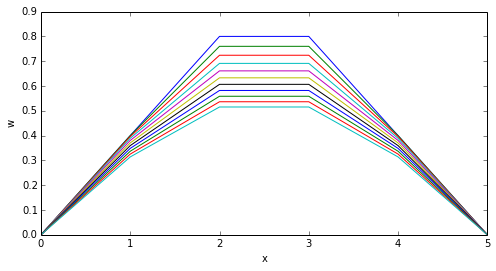
\includegraphics[width=0.5\textwidth]{HeatEquationFigures/r_equals_one_tenth/solution_plot_lines}
        \label{Plot_FTCS_1_10}

\end{figure}
Figure \ref{Color_FTCS_1_10} shows the explicit numerical solution $w$ of the Heat Equation for $r=\frac{1}{10}$ for $10$ time steps as a colour plot. 

\begin{figure}[H]
  \caption{The colour plot of the explicit numerical solution $w$ of the Heat Equation for $r=\frac{1}{10}$.}
  \centering
    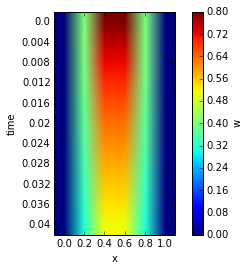
\includegraphics[width=0.5\textwidth]{HeatEquationFigures/r_equals_one_tenth/solution_plot_image}
    \label{Color_FTCS_1_10}
\end{figure}
The forward time and centered space numerical solution for the Heat Equation shown in Figures \ref{Color_FTCS_1_10} and  \ref{Plot_FTCS_1_10} tends to $0$ in a monotonic fashion as time progresses for $r=\frac{1}{10}$. 
\end{example}
\begin{example}
\subsubsection{Explicit FTCS method for the Heat Equation with $r=\frac{1}{2}$}
Let $h=\frac{1}{5}$ and $k=\frac{1}{50}$ so that $r=\frac{k}{h^2}=\frac{1}{2}$
difference equation (\ref{disc heat}) becomes
\[
w_{ij+1}=\frac{1}{2}(w_{i-1j}+w_{i+1j}).
\]
This can be written in matrix form 
\[
\left(\begin{array}{c}
w_{1j+1}\\
w_{2j+1}\\
w_{3j+1}\\
w_{4j+1}
\end{array}\right)
=
\left(\begin{array}{cccc}
0.0&0.5&0&0\\
0.5&0.0&0.5&0\\
0&0.5&0.0&0.5\\
0&0&0.5&0.0
\end{array}\right)
\left(\begin{array}{c}
w_{1j}\\
w_{2j}\\
w_{3j}\\
w_{4j}
\end{array}\right)
+0.5\left(\begin{array}{c}
w_{0j}\\
0\\
0\\
w_{Nj}
\end{array}\right).
\]
Figure \ref{Matrix_FTCS_1_2} is a graphical representation of the matrix A. 
\begin{figure}[H]
  \caption{Graphical representation of the matrix A for $r=\frac{1}{2}$. }
  \centering
    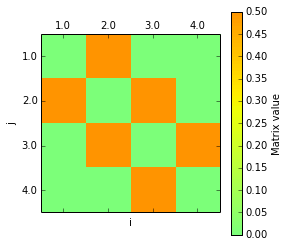
\includegraphics[width=0.5\textwidth]{HeatEquationFigures/r_equals_half/Matrix}
    \label{Matrix_FTCS_1_2}
\end{figure}

Table \ref{Matrix_FTCS_1_2} shows the explicit numerical solution $w$ of the Heat Equation for $r=\frac{1}{2}$ for $1$ time step.


\begin{center}
\begin{table}[H]
 \caption{The explicit numerical solution $w$ of the Heat Equation for $r=\frac{1}{2}$ for $1$ time step.}
     \label{Table_FTCS_1_2}
 \centering
\begin{tabular}{l|cccccc}
t/x&0&0.2&0.4&0.6&0.8&1.0\\ \hline
0&0&0.4&0.8&0.8&0.4&0.0\\
$\frac{1}{50}$&0&0.4&0.6&0.6&0.4&0.0\\
\end{tabular}
\end{table}
\end{center}

Figure \ref{Plot_FTCS_1_2} shows the explicit numerical solution $w$ of the Heat Equation for $r=\frac{1}{2}$ for $10$ time steps each represented by a different line.
\begin{figure}[H]
  \caption{The explicit numerical solution $w$ of the Heat Equation for $r=\frac{1}{2}$ for $10$ time steps each represented by a different line.}
  \centering
    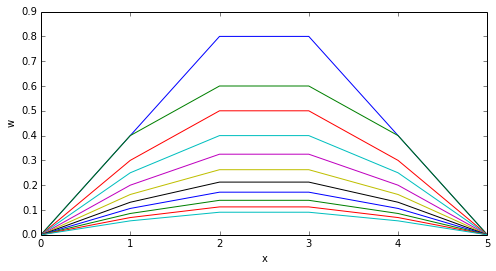
\includegraphics[width=0.5\textwidth]{HeatEquationFigures/r_equals_half/solution_plot_lines}     \label{Plot_FTCS_1_2}

\end{figure}
Figure \ref{Color_FTCS_1_2} shows the explicit numerical solution $w$ of the Heat Equation for $r=\frac{1}{2}$ for $10$ time steps as a colour plot.

\begin{figure}[H]
  \caption{The colour plot of the explicit numerical solution $w$ of the Heat Equation for $r=\frac{1}{2}$.}
  \centering
    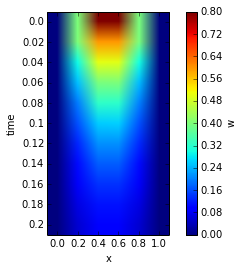
\includegraphics[width=0.5\textwidth]{HeatEquationFigures/r_equals_half/solution_plot_image}\label{Color_FTCS_1_2}
\end{figure}


The choice of $r=\frac{1}{2}$  gives an acceptable approximation to the solution of the \addtoindex{Heat Equation} as shown in Figures  \ref{Plot_FTCS_1_2} and \ref{Color_FTCS_1_2}.
\end{example}
\begin{example}
\subsubsection{Explicit FTCS method for the Heat Equation with $r=1$}
Let $h=\frac{1}{5}$ and $k=\frac{1}{25}$ so that $r=\frac{k}{h^2}=1$
difference equation (\ref{disc heat}) becomes
\[
w_{ij+1}=w_{i-1j}-w_{ij}+w_{i+1j}.
\]
This can be written in matrix form 
\[
\left(\begin{array}{c}
w_{1j+1}\\
w_{2j+1}\\
w_{3j+1}\\
w_{4j+1}
\end{array}\right)
=
\left(\begin{array}{cccc}
-1.0&1.0&0&0\\
1.0&-1.0&1.0&0\\
0&1.0&-1.0&1.0\\
0&0&1.0&-1.0
\end{array}\right)
\left(\begin{array}{c}
w_{1j}\\
w_{2j}\\
w_{3j}\\
w_{4j}
\end{array}\right)\]\[+\left(\begin{array}{c}
w_{0j}\\
0\\
0\\
w_{5j}
\end{array}\right).
\]
\begin{figure}[H]
  \caption{Graphical representation of the matrix A for $r=1$.}
  \centering
    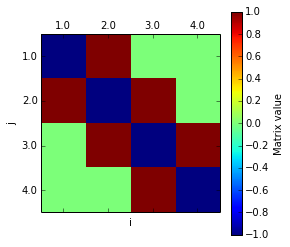
\includegraphics[width=0.5\textwidth]{HeatEquationFigures/r_equals_one/Matrix}
\end{figure}


\begin{center}
\begin{table}[H]
 \caption{The explicit numerical solution $w$ of the Heat Equation for $r=1$ for 3 time steps.}
 \centering
\begin{tabular}{l|cccccc}
t/x&0&0.2&0.4&0.6&0.8&1.0\\ \hline
0&0&0.4&0.8&0.8&0.4&0.0\\
$\frac{1}{25}$&0&0.4&0.4&0.4&0.4&0.0\\
$\frac{2}{25}$&0&0.0&0.4&0.4&0.0&0.0\\
$\frac{3}{25}$&0&0.4&0.0&0.0&0.4&0.0\\
\end{tabular}
\end{table}
\end{center}

\begin{figure}[H]
  \caption{The explicit numerical solution $w$ of the Heat Equation for $r=1$ for 10 time steps each represented by a different line.}
  \centering
    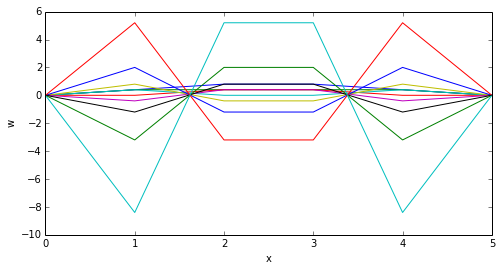
\includegraphics[width=0.5\textwidth]{HeatEquationFigures/r_equals_one/solution_plot_lines}
\end{figure}


\begin{figure}[H]
  \caption{The colorplot of The explicit numerical solution $w$ of the Heat Equation for $r=1$.}
  \centering
    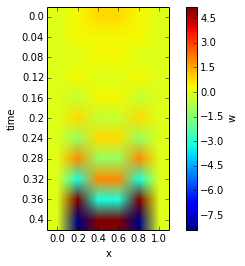
\includegraphics[width=0.5\textwidth]{HeatEquationFigures/r_equals_one/solution_plot_image}
\end{figure}

Considered as a solution to the \addtoindex{Heat Equation} this is meaningless although it is the correct
solution of the difference equation with respect to the initial conditions and the boundary conditions.
\end{example}
\section{An implicit (BTCS) method for the Heat Equation}
The  implicit Backward Time Centered Space (BTCS) difference equation of the differential Heat equation (\ref{heat}) is
\begin{equation}
\frac{w_{ij+1}-w_{ij}}{k}=\frac{w_{i+1j+1}-2w_{ij+1}+w_{i-1j+1}}{h^2}
\end{equation}
when approaching this we have divided up the area into
two uniform meshes one in the $x$ direction and the other in the $t$-direction.
We define $t_j=jk$ where $k$ is the step size in the time direction.\\
We define $x_i=ih$ where $h$ is the step size in the space direction.\\
$w_{ij}$ denotes the numerical approximation of $U$ at $(x_i,t_j)$.\\
Rearranging the equation we get
\begin{equation}\label{disc heat imp}
-rw_{i-1j+1}+(1+2r)w_{ij+1}-rw_{i+1j+1}=w_{ij}
\end{equation}
where $r=\frac{k}{h^2}$.\\
This gives the formula for the unknown term $w_{ij+1}$ at the $(ij+1)$ mesh points
in terms of terms along the jth time row.\\
Hence we can calculate the unknown pivotal values of $w$ along the first row $t=k$ or $j=1$ in terms of the known boundary conditions.\\
This can be written in matrix from 
\[ A\mathbf{w}_{j+1}=\mathbf{w}_{j} +\mathbf{b}_{j+1} \]
for which $A$ is
\[
\left(\begin{array}{ccccccc}
1+2r&-r&0&.&.&.&.\\
-r&1+2r&-r&0&.&.&.\\
0&-r&1+2r&-r&0&.&.\\
.&.&.&.&.&.&.\\
.&.&.&.&-r&1+2r&-r\\
.&.&.&.&.&-r&1+2r\\
\end{array}\right)
\]
where $r=\frac{k}{h_x^2}>0$, $\mathbf{w}_j$ is 
\[
\left(\begin{array}{c}
w_{1j}\\
w_{2j}\\
.\\
w_{N-2j}\\
w_{N-1j}\\

\end{array}\right)
\]
and $\mathbf{b}_{j+1}$ is 
\[
\left(\begin{array}{c}
rw_{0j+1}\\
0\\
.\\
0\\
rw_{Nj+1}\\
\end{array}\right).
\]
It is assumed that the boundary values $w_{0j}$ and $w_{Nj}$ are known for $j=1,2,...$, and $w_{i0}$ is the initial condition.

\subsection{Example implicit (BTCS) for the Heat Equation} 
In this case we look at a rod of unit length with each end in ice.\\
The rod is heat insulated along its length so that temperature changes occur through
heat conduction along its length and heat transfer at its ends, where $w$ denotes
temperature.\\
Given that the ends of the rod are kept in contact with ice and the initial temperature
distribution is non dimensional form is
\begin{enumerate}
\item $U=2x$ for $0\leq x \leq \frac{1}{2}$ 
\item $U=2(1-x)$ for $\frac{1}{2}\leq x \leq 1$ 
\end{enumerate}
In other words we are seeking a numerical solution of
\[\frac{\partial U}{\partial t}=\frac{\partial^2U }{\partial x^2}\]
which satisfies
\begin{enumerate}
\item $U=0$ at $x=0$ for all $t>0$ (the boundary condition),
\item $U=2x$ for $0\leq x \leq \frac{1}{2}$ for $t=0$,\\
$U=2(1-x)$ for $\frac{1}{2}\leq x \leq 1$ for $t=0$ (the initial condition).
\end{enumerate}
\begin{example}
\subsubsection{Implicit (BTCS) method for the Heat Equation  $r=\frac{1}{10}$}
Let $h=\frac{1}{5}$ and $k=\frac{1}{250}$ so that $r=\frac{k}{h^2}=\frac{1}{10}$
difference equation (\ref{disc heat}) becomes
\[
\frac{1}{10}(-w_{i-1j+1}+(12)w_{ij+1}-w_{i+1j+1})=w_{ij}
\]
This can be written in matrix form 
\[
\left(\begin{array}{cccc}
1.2&-0.1&0&0\\
-0.1&1.2&-0.1&0\\
0&-0.1&1.2&-0.1\\
0&0&-0.1&1.2
\end{array}\right)
\left(\begin{array}{c}
w_{1j+1}\\
w_{2j+1}\\
w_{3j+1}\\
w_{4j+1}
\end{array}\right)
=
\left(\begin{array}{c}
w_{1j}\\
w_{2j}\\
w_{3j}\\
w_{4j}
\end{array}\right)+0.1\left(\begin{array}{c}
w_{0j+1}\\
0\\
0\\
w_{5j+1}
\end{array}\right).
\]
\begin{figure}[H]
  \caption{Graphical representation of the matrix A for $r=\frac{1}{10}$. }
  \centering
    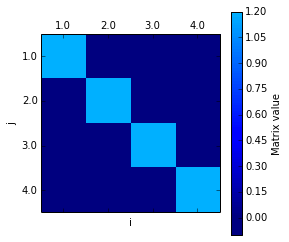
\includegraphics[width=0.5\textwidth]{HeatEquationFigures/Fully_implicit/r_equals_one_tenth/Matrix}
\end{figure}


To solve we need to invert the matix, to get
\[ \mathbf{w}_{j+1}=A^{-1}(\mathbf{w}_{j} +\mathbf{b}_{j}) \]


\begin{center}
 \begin{table}[H]
 \caption{The implicit numerical solution $w$ of the Heat Equation for $r=\frac{1}{10}$ for 1 time step.}
 \centering
\begin{tabular}{l|cccccc}
j/x&0&0.2&0.4&0.6&0.8&1.0\\ \hline
0&0&0.4&0.8&0.8&0.4&0.0\\
$\frac{1}{250}$&
 0.&          0.39694656 & 0.76335878 & 0.76335878 & 0.39694656&  0.
\end{tabular}
\end{table}
\end{center}

\begin{figure}[H]
  \caption{The implicit numerical solution $w$ of the Heat Equation for $r=\frac{1}{10}$ for $10$ time steps each represented by a different line.}
  \centering
    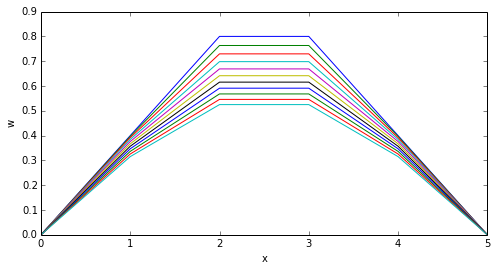
\includegraphics[width=0.5\textwidth]{HeatEquationFigures/Fully_implicit/r_equals_one_tenth/solution_plot_lines}
\end{figure}


\begin{figure}[H]
  \caption{The colorplot of The implicit numerical solution $w$ of the Heat Equation for $r=\frac{1}{10}$.}
  \centering
    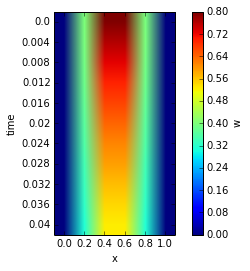
\includegraphics[width=0.5\textwidth]{HeatEquationFigures/Fully_implicit/r_equals_one_tenth/solution_plot_image}
\end{figure}
\end{example}

\begin{example}


\subsubsection{Implicit (BTCS) method for the Heat Equation for $r=\frac{1}{2}$}
Let $h=\frac{1}{5}$ and $k=\frac{1}{50}$ so that $r=\frac{k}{h^2}=\frac{1}{2}$
difference equation (\ref{disc heat}) becomes
\[
\frac{1}{2}(-w_{i-1j+1}+(4)w_{ij+1}-w_{i+1j+1})=w_{ij}
\]
This can be written in matrix form 
\[
\left(\begin{array}{cccc}
2&-0.5&0&0\\
-0.5&2&-0.5&0\\
0&-0.5&2&-0.5\\
0&0&-0.5&2
\end{array}\right)
\left(\begin{array}{c}
w_{1j+1}\\
w_{2j+1}\\
w_{3j+1}\\
w_{4j+1}
\end{array}\right)
=
\left(\begin{array}{c}
w_{1j}\\
w_{2j}\\
w_{3j}\\
w_{4j}
\end{array}\right).
\]
\begin{figure}[H]
  \caption{Graphical representation of the matrix A for $r=\frac{1}{2}$ }
  \centering
    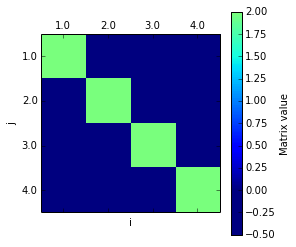
\includegraphics[width=0.5\textwidth]{HeatEquationFigures/Fully_implicit/r_equals_half/Matrix}
\end{figure}


\begin{center}
\begin{table}[H]
 \caption{The implicit numerical solution $w$ of the Heat Equation for $r=\frac{1}{2}$ for $1$ time step}
 \centering
\begin{tabular}{l|cccccc}
t/x&0&0.2&0.4&0.6&0.8&1.0\\ \hline
0&0&0.4&0.8&0.8&0.4&0.0\\
$\frac{1}{50}$&0. &         0.36363636 &  0.65454545 & 0.65454545&  0.36363636 & 0.
\end{tabular}
\end{table}
\end{center}

\begin{figure}[H]
  \caption{The implicit numerical solution $w$ of the Heat Equation for $r=\frac{1}{2}$ for $10$ time steps each represented by a different line}
  \centering
    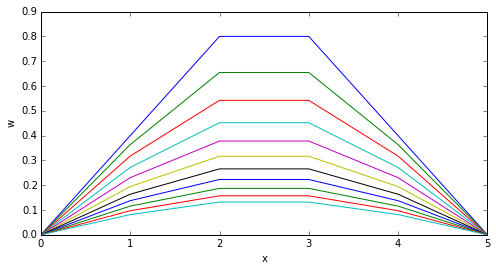
\includegraphics[width=0.5\textwidth]{HeatEquationFigures/Fully_implicit/r_equals_half/solution_plot_lines}
\end{figure}


\begin{figure}[H]
  \caption{The colorplot of the implicit numerical solution $w$ of the Heat Equation for $r=\frac{1}{2}$.}
  \centering
    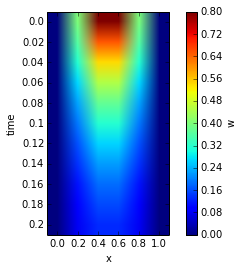
\includegraphics[width=0.5\textwidth]{HeatEquationFigures/Fully_implicit/r_equals_half/solution_plot_image}
\end{figure}


This method also gives an acceptable approximation to the solution of the \addtoindex{PDE}.
\end{example}
\begin{example}
\subsubsection{Implicit (BTCS) method for the Heat Equation for $r=1$}
Let $h=\frac{1}{5}$ and $k=\frac{1}{25}$ so that $r=\frac{k}{h^2}=1$
difference equation (\ref{disc heat}) becomes
\[
(-w_{i-1j+1}+(3)w_{ij+1}-w_{i+1j+1})=w_{ij}
\]
This can be written in matrix form 
\[
\left(\begin{array}{cccc}
3&-1&0&0\\
-1&3&-1&0\\
0&-1&3&-1\\
0&0&-1&3
\end{array}\right)
\left(\begin{array}{c}
w_{1j+1}\\
w_{2j+1}\\
w_{3j+1}\\
w_{4j+1}
\end{array}\right)
=
\left(\begin{array}{c}
w_{1j}\\
w_{2j}\\
w_{3j}\\
w_{4j}
\end{array}\right)+\left(\begin{array}{c}
w_{0j+1}\\
0\\
0\\
w_{5j+1}
\end{array}\right).
\]
\begin{figure}[H]
  \caption{Graphical representation of the matrix A for $r=1$ }
  \centering
    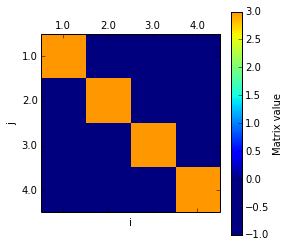
\includegraphics[width=0.5\textwidth]{HeatEquationFigures/Fully_implicit/r_equals_one/Matrix}
\end{figure}


\begin{center}
\begin{table}[H]
 \caption{The implicit numerical solution $w$ of the Heat Equation for $r=1$ for 3 time step}
 \centering
\begin{tabular}{l|cccccc}
t/x&0&0.2&0.4&0.6&0.8&1.0\\ \hline
0&0&0.4&0.8&0.8&0.4&0.0\\
$\frac{1}{25}$&0.  &  0.32  &0.56&  0.56 & 0.32  &0.\\
$\frac{2}{25}$&0. &   0.24 & 0.4  & 0.4  & 0.24 & 0.\\
$\frac{3}{25}$&0. &    0.176&  0.288 & 0.288 & 0.176 & 0. 
\end{tabular}
\end{table}
\end{center}

\begin{figure}[H]
  \caption{The implicit numerical solution $w$ of the Heat Equation for $r=1$ for 10 time steps each represented by a different line}
  \centering
    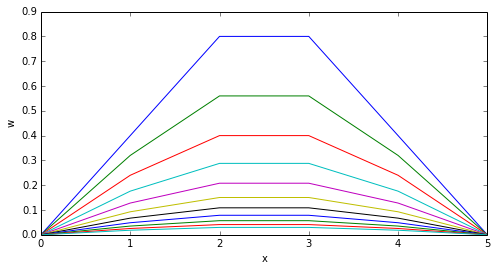
\includegraphics[width=0.5\textwidth]{HeatEquationFigures/Fully_implicit/r_equals_one/solution_plot_lines}
\end{figure}


\begin{figure}[H]
  \caption{The colorplot of the implicit numerical solution $w$ of the Heat Equation for $r=1$.}
  \centering
    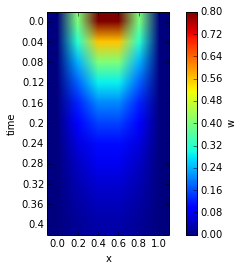
\includegraphics[width=0.5\textwidth]{HeatEquationFigures/Fully_implicit/r_equals_one/solution_plot_image}
\end{figure}
\end{example}


\section{Crank Nicholson Implicit method}
Since the implicit method requires that $k\leq \frac{1}{2}h^2$ a new method was
needed which would work for all finite values of r.\\
They considered the partial differential equation as being satisfied at the
midpoint $\{ih,(j+\frac{1}{2})k \}$ and replace $\frac{\delta^2 U}{\delta x^2}$ by the
mean of its finite difference approximations at the jth and (j+1)th time levels.
In other words they approximated the equation
\[ \left(\frac{\delta U}{\delta t}\right)_{i,j+\frac{1}{2}}
= 
 \left(\frac{\delta^2 U}{\delta x^2}\right)_{i,j+\frac{1}{2}}\]
by
\[\frac{w_{i,j+1}-w_{ij}}{k}=\frac{1}{2}\left\{\frac{w_{i+1j+1}-2w_{ij+1}+w_{i-1j+1}}{h^2}+
\frac{w_{i+1j}-2w_{ij}+w_{i-1j}}{h^2}
\right\}
\]
giving
\begin{equation}
\label{2 crank}
-rw_{i-1j+1}+(2+2r)w_{ij+1}-rw_{i+1j+1}
=
rw_{i-1j}+(2-2r)w_{ij}+rw_{i+1j}
\end{equation}

with $r=\frac{k}{h^2}$.\\
In general the LHS contains $3$ unknowns and the RHS $3$ known pivotal values.\\
If there are N intervals mesh points along each row then for $j=0$ and $i=1,..,N$ it 
gives N simultaneous equations for $N$ unknown pivotal values along the first row.\\
Which can be described in matrix form 
\[ B \mathbf{w}_{j+1}=C\mathbf{w}_{j}+\mathbf{b}_{j}\]
as
\begin{eqnarray*}
\left(\begin{array}{ccccccc}
2+2r&-r&0&.&.&.&.\\
-r&2+2r&-r&0&.&.&.\\
0&-r&2+2r&-r&0&.&.\\
.&.&.&.&.&.&.\\
.&.&.&.&-r&2+2r&-r\\
.&.&.&.&.&-r&2+2r\\
\end{array}\right)
\left(\begin{array}{c}
w_{1j+1}\\
w_{2j+1}\\
.\\
.\\
w_{N-2j+1}\\
w_{N-1j+1}\\
\end{array}\right)\\
=
\left(\begin{array}{ccccccc}
2-2r&r&0&.&.&.&.\\
r&2-2r&r&0&.&.&.\\
0&r&2-2r&r&0&.&.\\
.&.&.&.&.&.&.\\
.&.&.&.&r&2-2r&r\\
.&.&.&.&.&r&2-2r\\
\end{array}\right)
\left(\begin{array}{c}
w_{1j}\\
w_{2j}\\
.\\
.\\
w_{N-2j}\\
w_{N-1j}\\
\end{array}\right)
+\mathbf{b}_j+\mathbf{b}_{j+1}
\end{eqnarray*}
where $\mathbf{b}_j$ and $\mathbf{b}_{j+1}$ are vectors of known boundary conditions. 
\begin{equation}
    \mathbf{b}_j=\left(\begin{array}{c}
rw_{0j}\\
0\\
.\\
.\\
0\\
rw_{Nj}\\
\end{array}\right), \ \ \     
\mathbf{b}_{j+1}=\left(\begin{array}{c}
rw_{0j+1}\\
0\\
.\\
.\\
0\\
rw_{Nj+1}\\
\end{array}\right)
\end{equation}

\subsection{Example Crank-Nicholson solution of the Heat Equation} 
In this case we look at a rod of unit length with each end in ice.\\
The rod is heat insulated along its length so that temperature changes occur through
heat conduction along its length and heat transfer at its ends, where w denotes
temperature.\\
\textbf{Simple case}\\
Given that the ends of the rod are kept in contact with ice and the initial temperature
distribution is non dimensional form is
\begin{enumerate}
\item $U=2x$ for $0\leq x \leq \frac{1}{2}$ 
\item $U=2(1-x)$ for $\frac{1}{2}\leq x \leq 1$ 
\end{enumerate}
In other words we are seeking a numerical solution of
\[\frac{\partial U}{\partial t}=\frac{\partial^2U }{\partial x^2}\]
which satisfies
\begin{enumerate}
\item $U=0$ at $x=0$ for all $t>0$ (the boundary condition)
\item $U=2x$ for $0\leq x \leq \frac{1}{2}$ for $t=0$
$U=2(1-x)$ for $\frac{1}{2}\leq x \leq 1$ for $t=0$ (the initial condition)
\end{enumerate}
\begin{example}
\subsubsection{Crank-Nicholson method $r=\frac{1}{10}$}
Let $h=\frac{1}{5}$ and $k=\frac{1}{250}$ so that $r=\frac{k}{h^2}=\frac{1}{10}$
difference equation (\ref{2 crank}) becomes
\[-0.1w_{i-1,j+1}+2.2w_{i,j+1}-0.1w_{i+1,j+1}=0.1w_{i-1,j}+1.8w_{i,j}+0.1w_{i+1,j} \]
Let $j=0$
\[\begin{array}{lcl}
i=1:& &\\
-0.1w_{0,1}+2.2w_{1,1}-0.1w_{2,1}&=&0.1w_{0,0}+1.8w_{1,0}+0.1w_{2,0}\\
i=2:& &\\
-0.1w_{1,1}+2.2w_{2,1}-0.1w_{3,1}&=&0.1w_{1,0}+1.8w_{2,0j}+0.1w_{3,0}\\
i=3:& &\\
-0.1w_{2,1}+2.2w_{3,1}-0.1w_{4,1}&=&0.1w_{2,0}+1.8w_{3,0}+0.1w_{4,0}\\
i=4:& &\\
-0.1w_{3,1}+2.2w_{4,1}-0.1w_{5,1}&=&0.1w_{3,0}+1.8w_{4,0}+0.1w_{5,0}
\end{array}\]
In matrix form
\[\left(\begin{array}{cccc}
2.2&-0.1&0&0\\
-0.1&2.2&-0.1&0\\
0&-0.1&2.2&-0.1\\
0&0&-0.1&2.2
\end{array}
\right)
\left(\begin{array}{c}
w_{1,1}\\
w_{2,1}\\
w_{3,1}\\
w_{4,1}\\
\end{array}
\right)\]\[=\left(\begin{array}{cccc}
1.8&0.1&0&0\\
0.1&1.8&0.1&0\\
0&0.1&1.8&0.1\\
0&0&0.1&1.8\\

\end{array}
\right)
\left(\begin{array}{c}
w_{1,0}\\
w_{2,0}\\
w_{3,0}\\
w_{4,0}
\end{array}
\right)+0.1
\left(\begin{array}{c}
w_{0,1}+w_{0,0}\\
0\\
0\\
w_{5,1}+w_{5,0}\\
\end{array}
\right)
\]	

To solve we need to invert the matix, to get
\[ \mathbf{w}_{j+1}=A^{-1}(B\mathbf{w}_{j} +\mathbf{b}_{j+1}+\mathbf{b}_{j}) \]


\begin{center}
 \begin{table}[H]
 \caption{The Crank-Nicholson numerical solution $w$ of the Heat Equation for $r=\frac{1}{10}$ for 1 time step}
 \centering
\begin{tabular}{l|cccccc}
j/x&0&0.2&0.4&0.6&0.8&1.0\\ \hline
0&0&0.4&0.8&0.8&0.4&0.0\\
$\frac{1}{250}$&
 0.   &       0.39826464  &0.76182213 & 0.76182213 & 0.39826464&  0.
\end{tabular}
\end{table}
\end{center}

\begin{figure}[H]
  \caption{The Crank-Nicholson numerical solution $w$ of the Heat Equation for $r=\frac{1}{10}$ for 10 time steps each represented by a different line}
  \centering
    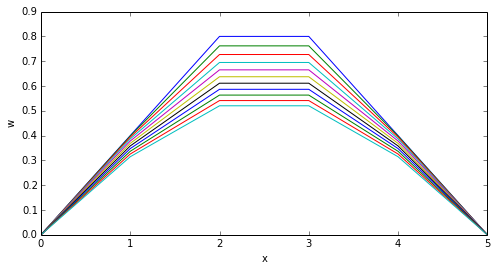
\includegraphics[width=0.5\textwidth]{HeatEquationFigures/CRN/r_equals_one_tenth/solution_plot_lines}
\end{figure}


\begin{figure}[H]
  \caption{The colorplot of the Crank-Nicholson numerical solution $w$ of the Heat Equation for $r=\frac{1}{10}$.}
  \centering
    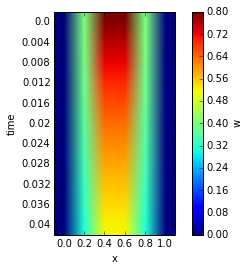
\includegraphics[width=0.5\textwidth]{HeatEquationFigures/CRN/r_equals_one_tenth/solution_plot_image}
\end{figure}

\end{example}
\begin{example}
\subsubsection{Crank-Nicholson method $r=\frac{1}{2}$}
Let $h=\frac{1}{5}$ and $k=\frac{1}{50}$ so that $r=\frac{k}{h^2}=\frac{1}{2}$
difference equation (\ref{2 crank}) becomes
\[-0.5w_{i-1,j+1}+3w_{i,j+1}-0.5w_{i+1,j+1}=\]
\[
0.5w_{i-1,j}+1w_{i,j}+0.5w_{i+1,j} \]
Let $j=0$
\[\begin{array}{lcl}
i=1:&\\
-0.5w_{0,1}+3w_{1,1}-0.5w_{2,1}&=&0.5w_{0,0}+1w_{1,0}+0.5w_{2,0}\\
i=2:&\\
-0.5w_{1,1}+3w_{2,1}-0.5w_{3,1}&=&0.5w_{1,0}+1w_{2,0j}+0.5w_{3,0}\\
i=3:&\\
-0.5w_{2,1}+3w_{3,1}-0.5w_{4,1}&=&0.5w_{2,0}+1w_{3,0}+0.5w_{4,0}\\
i=4:&\\
-0.5w_{3,1}+3w_{4,1}-0.5w_{5,1}&=&0.5w_{3,0}+1w_{4,0}+0.5w_{5,0}
\end{array}\]
In matrix form
\[\left(\begin{array}{cccc}
3&-0.5&0&0\\
-0.5&3&-0.5&0\\
0&-0.5&3&-0.5\\
0&0&-0.5&3
\end{array}
\right)
\left(\begin{array}{c}
w_{1,1}\\
w_{2,1}\\
w_{3,1}\\
w_{4,1}\\
\end{array}
\right)=\]\
\[\left(\begin{array}{cccc}
1&0.5&0&0\\
0.5&1&0.5&0\\
0&0.5&1&0.5\\
0&0&0.5&1\\

\end{array}
\right)
\left(\begin{array}{c}
w_{1,0}\\
w_{2,0}\\
w_{3,0}\\
w_{4,0}
\end{array}
\right)+0.5
\left(\begin{array}{c}
w_{0,1}+w_{0,0}\\
0\\
0\\
w_{5,1}+w_{5,0}\\
\end{array}
\right)
\]	



\begin{center}
\begin{table}[H]
 \caption{The Crank-Nicholson numerical solution $w$ of the Heat Equation for $r=\frac{1}{2}$ for 1 time step}
 \centering
\begin{tabular}{l|cccccc}
t/x&0&0.2&0.4&0.6&0.8&1.0\\ \hline
0&0&0.4&0.8&0.8&0.4&0.0\\
$\frac{1}{50}$&0.    &      0.37241379  & 0.63448276 & 0.63448276  & 0.37241379 & 0.
\end{tabular}
\end{table}
\end{center}

\begin{figure}[H]
  \caption{The Crank-Nicholson numerical solution $w$ of the Heat Equation for $r=\frac{1}{2}$ for 10 time steps each represented by a different line}
  \centering
    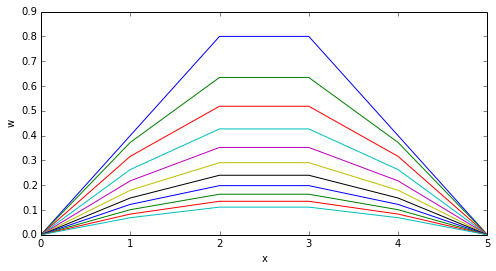
\includegraphics[width=0.5\textwidth]{HeatEquationFigures/CRN/r_equals_half/solution_plot_lines}
\end{figure}


\begin{figure}[H]
  \caption{The colorplot of the Crank-Nicholson numerical solution $w$ of the Heat Equation for $r=\frac{1}{2}$.}
  \centering
    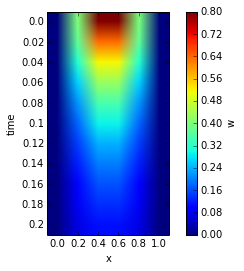
\includegraphics[width=0.5\textwidth]{HeatEquationFigures/CRN/r_equals_half/solution_plot_image}
\end{figure}


This method also gives an good approximation to the solution of the \addtoindex{PDE}.
\end{example}
\begin{example}

\subsubsection{Crank-Nicholson method for the Heat Equation with  $r=1$}
Let $h=\frac{1}{5}$ and $k=\frac{1}{25}$ so that $r=\frac{k}{h^2}=1$
difference equation (\ref{2 crank}) becomes
\[-w_{i-1,j+1}+4w_{i,j+1}-w_{i+1,j+1}=w_{i-1,j}+0w_{i,j}+w_{i+1,j} \]
Let $j=0$
\[\begin{array}{lcl}
i=1:& &\\
-w_{0,1}+4w_{1,1}-w_{2,1}&=&w_{0,0}+0w_{1,0}+w_{2,0}\\
i=2:& &\\
-w_{1,1}+4w_{2,1}-w_{3,1}&=&w_{1,0}+0w_{2,0j}+w_{3,0}\\
i=3:& &\\
-w_{2,1}+4w_{3,1}-w_{4,1}&=&w_{2,0}+0w_{3,0}+w_{4,0}\\
i=4:& &\\
-w_{3,1}+4w_{4,1}-w_{5,1}&=&w_{3,0}+0w_{4,0}+w_{5,0}
\end{array}\]
In matrix form
\[\left(\begin{array}{cccc}
4&-1&0&0\\
-1&4&-1&0\\
0&-1&4&-1\\
0&0&-1&4
\end{array}
\right)
\left(\begin{array}{c}
w_{1,1}\\
w_{2,1}\\
w_{3,1}\\
w_{4,1}\\
\end{array}
\right)\]
\[=\left(\begin{array}{cccc}
0&1&0&0\\
1&0&1&0\\
0&1&0&1\\
0&0&1&0\\

\end{array}
\right)
\left(\begin{array}{c}
w_{1,0}\\
w_{2,0}\\
w_{3,0}\\
w_{4,0}
\end{array}
\right)+
\left(\begin{array}{c}
w_{0,1}+w_{0,0}\\
0\\
0\\
w_{5,1}+w_{5,0}\\
\end{array}
\right)
\]	




\begin{center}
\begin{table}[H]
 \caption{The Crank-Nicholson numerical solution $w$ of the Heat Equation for $r=1$ for 3 time step}
 \centering
\begin{tabular}{l|cccccc}
t/x&0&0.2&0.4&0.6&0.8&1.0\\ \hline
0&0&0.4&0.8&0.8&0.4&0.0\\
$\frac{1}{25}$&0.  &        0.32727273&  0.50909091 & 0.50909091&  0.32727273&  0.\\
$\frac{2}{25}$&0.      &    0.21487603 & 0.35041322 & 0.35041322&  0.21487603 & 0.\\

$\frac{3}{25}$&0.    &      0.14695718&  0.23741548  &0.23741548&  0.14695718&  0. 
\end{tabular}
\end{table}
\end{center}

\begin{figure}[H]
  \caption{The Crank-Nicholson numerical solution $w$ of the Heat Equation for $r=1$ for 10 time steps each represented by a different line}
  \centering
    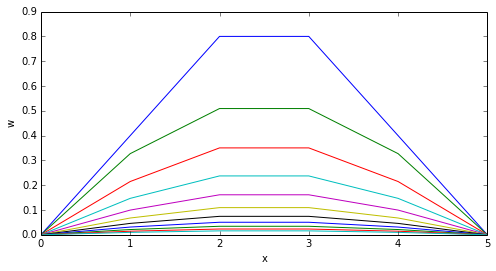
\includegraphics[width=0.5\textwidth]{HeatEquationFigures/CRN/r_equals_one/solution_plot_lines}
\end{figure}


\begin{figure}[H]
  \caption{The colorplot of the Crank-Nicholson numerical solution $w$ of the Heat Equation for $r=1$.}
  \centering
    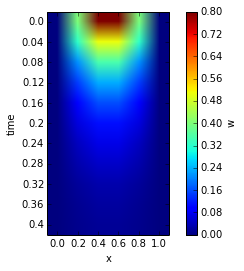
\includegraphics[width=0.5\textwidth]{HeatEquationFigures/CRN/r_equals_one/solution_plot_image}
\end{figure}

\end{example}




\section{The Theta Method}
The Theta Method is a generalization of the Crank-Nicholson method and expresses
our partial differential equation as
\begin{equation}
\label{2 theta}
\frac{w_{i,j+1}-w_{ij}}{k}=\left\{\theta\left(\frac{w_{i+1j+1}-2w_{ij+1}+w_{i-1j+1}}{h^2}\right)+
(1-\theta)\left(
\frac{w_{i+1j}-2w_{ij}+w_{i-1j}}{h^2}
\right)
\right\}
\end{equation}
\begin{itemize}
\item
when $\theta=0$ we get the explicit scheme,
\item
when $\theta=\frac{1}{2}$ we get the Crank-Nicholson scheme,
\item
and $\theta=1$ we get fully implicit backward finite difference method.
\end{itemize}
The equations are unconditionally valid for $\frac{1}{2}\leq \theta \leq 1$.
For  $0\leq \theta < \frac{1}{2}$ we must have
\[r\leq \frac{1}{2(1-2\theta)}. \]
\section{The General Matrix form}
Let the solution domain of the \addtoindex{PDE} be the finite rectangle $0\leq x \leq 1$ and
$0\leq t \leq T$ and subdivide it into a uniform rectangular mesh by the lines
$x_i=ih$ for $i=0$ to $N$ and $t_{j}=jk$ for $j=0$ to $J$ it will be assumed that $h$ is related to $k$ by some relationship such as $k=rh$ or $k=rh^2$ with $r>0$ and finite so that as $h\rightarrow 0$ as $k \rightarrow 0$.\\
Assume that the finite difference equation relating the mesh point values along the $(j+1)$th and jth row is 
\[b_{i-1}w_{i-1j+1}+
b_{i}w_{ij+1}+
b_{i+1}w_{i+1j+1}
=
c_{i-1}w_{i-1j}+
c_{i}w_{ij}+
c_{i+1}w_{i+1j}\]
where the coefficients are constant. If the boundary values at $i=0$ and $N$ for $j>0$ are known these $(N-1)$ equations for $i=1$ to $N-1$ can be written in 
matrix form.
\begin{eqnarray*}
\left(\begin{array}{ccccccc}
b_1&b_2&0&.&.&.&.\\
b_1&b_2&b_3&0&.&.&.\\
0&b_2&b_3&b_4&0&.&.\\
.&.&.&.&.&.&.\\
.&.&.&.&b_{N-3}&b_{N-2}&b_{N-1}\\
.&.&.&.&.&b_{N-2}&b_{N-1}\\
\end{array}\right)
\left(\begin{array}{c}
w_{1j+1}\\
w_{2j+1}\\
.\\
.\\
w_{N-2j+1}\\
w_{N-1j+1}\\
\end{array}\right)
\\
=
\left(\begin{array}{ccccccc}
c_1&c_2&0&.&.&.&.\\
c_1&c_2&c_3&0&.&.&.\\
0&c_2&c_3&c_4&0&.&.\\
.&.&.&.&.&.&.\\
.&.&.&.&c_{N-3}&c_{N-2}&c_{N-1}\\
.&.&.&.&.&c_{N-2}&c_{N-1}\\
\end{array}\right)
\left(\begin{array}{c}
w_{1j}\\
w_{2j}\\
.\\
.\\
w_{N-2j}\\
w_{N-1j}\\
\end{array}\right)
+
\left(\begin{array}{c}
c_0w_{0j}-b_0w_{0j+1}\\
0\\
.\\
.\\
0\\
c_Nw_{Nj}-b_{N}w_{Nj+1}\\
\end{array}\right)
\end{eqnarray*}
Which can be written as
\[ B\mathbf{w}_{j+1}=C\mathbf{w}_j+\mathbf{d}_j \]
Where B and C are of order $(N-1)$ $\mathbf{w}_j$ denotes a column vector and
$\mathbf{d}_j$ denotes a column vector of boundary values.\\
Hence
\[ \mathbf{w}_{j+1}=B^{-1}C\mathbf{w}_j+B^{-1}\mathbf{d}_j. \]
Expressed in a more conventional manner as
\[ \mathbf{w}_{j+1}=A\mathbf{w}_j+\mathbf{f}_j \]
Where $A=B^{-1}C$ and $\mathbf{f}_j =B^{-1}\mathbf{d}_j$.  

\section{Derivative Boundary Conditions}
Boundary conditions expressed in terms of derivatives occur frequently.
\subsection{Example Derivative Boundary Conditions}
\[
\frac{\partial U}{\partial x} = H(U-v_0) \ \ \ at \ x=0\]
where H is a positive constant and $v_0$ is the surrounding temperature.\\

How do we deal with this type of boundary condition?\\

\begin{enumerate}
\item
By using forward difference for $\frac{\partial U}{\partial x}$, we have
\[
\frac{w_{1j}-w_{0j}}{h_x} = H(w_{0j}-v_0)\]
where $h_x=x_1-x_0$.  This gives us one extra equation for the temp $w_{ij}$.\\
\item
If we wish to represent $\frac{\partial U}{\partial x}$ more accurately at x=0, we use a central difference formula.  It is necessary to introduce a fictitious
temperature $w_{-1j}$ at the external mesh points $(-h_x,jk)$.  The temperature $w_{-1j}$ is unknown and needs another equation.  This is obtained by assuming that the heat 
conduction equation is satisfied at the end points.  The unknown $w_{-1j}$ can be 
eliminated between these equations.\\
\end{enumerate}
%{Example}\\
Solve for the equation
\[\frac{\partial U}{\partial t} =\frac{\partial^2 U}{\partial x^2} \]
satisfying the initial condition
\[U=1 \mbox{ for } 0\leq x \leq 1 \mbox{ when } t=0 \]
and the boundary conditions
\[\frac{\partial U}{\partial x} = U \mbox{ at } x=0 \mbox{ for all t} \]
\[\frac{\partial U}{\partial x} = -U \mbox{ at } x=1 \mbox{ for all t}. \]
\subsubsection{Example 1}
Using forward difference approximation for the derivative boundary condition
and the explicit method to approximate the \addtoindex{PDE}.\\
Our difference equation is,
\[
\frac{w_{i,j+1}-w_{ij}}{k}=
\frac{w_{i+1j}-2w_{ij}+w_{i-1j}}{h^2}
\]
\begin{equation}
\label{explicit forward}
w_{ij+1}=w_{ij} +r(w_{i-1j}-2w_{ij}+w_{i+1j})
\end{equation}
where $r=\frac{k}{h^{2}_x}$.\\
At i=1, (\ref{explicit forward}) is,
\begin{equation}
\label{explicit forward i=1}
w_{1j+1}=w_{1j} +r(w_{0j}-2w_{1j}+w_{2j})
\end{equation}
The boundary condition at $x=0$ is $\frac{\partial U}{\partial x} = U$ in terms of
forward difference this is 
\[ \frac{w_{1j}-w_{0j}}{h_x} = w_{0j}\]
rearranging 
\begin{equation}
\label{forward bc}
w_{0j}=\frac{w_{1j}}{1+h_x}
\end{equation}
Using (\ref{forward bc}) and (\ref{explicit forward i=1}) to eliminate we get,
\[w_{1j+1} = \left(1-2r+\frac{r}{1+h_x}\right)w_{1j}+rw_{2j}.\]


At $i=N-1$, (\ref{explicit forward}) is,
\begin{equation}
\label{explicit forward i=N-1}
w_{N-1j+1}=w_{N-1j} +r(w_{N-2j}-2w_{N-1j}+w_{Nj})
\end{equation}
The boundary condition at $x=1$ is $\frac{\partial U}{\partial x} = U$ in terms of
forward difference this is 
\[ \frac{w_{Nj}-w_{N-10}}{h_x} = w_{Nj}\]
rearranging 
\begin{equation}
\label{forward bc}
w_{Nj}=\frac{w_{N-1j}}{1-h_x}
\end{equation}
Using (\ref{forward bc}) and (\ref{explicit forward i=N-1}) to eliminate we get,
\[w_{N-1j+1} = rw_{N-2j}+\left(1-2r+\frac{r}{1-h_x}\right)w_{N-1j}.\]




Choose $h_s=\frac{1}{5}$ and $k=\frac{1}{100}$ such that $r=\frac{1}{4}$.\\
The equations become
\[w_{1j+1}=\frac{7}{24}w_{1j}+\frac{1}{4}w_{2j}, \]

\[w_{ij+1}=\frac{1}{4}(w_{i-1j}+2w_{ij}+w_{i+1j}) \ \ i=2,3 \]
and
\[w_{5j+1}=\frac{1}{4}w_{3j}+(\frac{13}{16}w_{4j}) \]

In matrix form

\[
\left(\begin{array}{c}
w_{1j+1}\\
w_{2j+1}\\
w_{3j+1}\\
w_{4j+1}
\end{array}\right)
=\left(\begin{array}{cccc}
\frac{7}{24}&\frac{1}{4}&0&0\\
\frac{1}{4}&\frac{1}{2}&\frac{1}{4}&0\\
0&\frac{1}{4}&\frac{1}{2}&\frac{1}{4}\\
0&0&\frac{1}{4}&\frac{13}{16}
\end{array}\right)
\left(\begin{array}{c}
w_{1j}\\
w_{2j}\\
w_{3j}\\
w_{4j}
\end{array}\right).
\]

with the boundaries given by
\[w_{0j+1}=\frac{10}{12}w_{1j+1},\]
\[w_{0j+1}=\frac{10}{8}w_{1j+1}.\]


\subsubsection{Example 2}
Using central difference approximation for the derivative boundary condition
and the explicit method to approximate the \addtoindex{PDE}.\\
Our difference equation is as in (\ref{explicit forward}).\\
At $i=0$ we have
\begin{equation}
\label{explicit central}
w_{0j+1}=w_{0j} +r(w_{-1j}-2w_{0j}+w_{1j})
\end{equation}
The boundary condition at $x=0$, in terms of central differences can be written as
\begin{equation}
\label{boundary central}
\frac{w_{1j}-w_{-1j}}{2h_x}=w_{0j} 
\end{equation}
Using (\ref{boundary central}) and (\ref{explicit central}) to eliminate the fictitious term $w_{-1j}$ we get,
\[
w_{0j+1}=w_{0j} +2r((-1-h_x)w_{0j}+w_{1j})
\]
\subsubsection{Example 3}
Using central difference approximation for the derivative boundary condition
and the Crank-Nicholson method to approximate the \addtoindex{PDE}.\\
The difference equation is,
\[\frac{w_{i,j+1}-w_{ij}}{k}=\frac{1}{2}\left\{\frac{w_{i+1j+1}-2w_{ij+1}+w_{i-1j+1}}{h^2}+
\frac{w_{i+1j}-2w_{ij}+w_{i-1j}}{h^2}
\right\}
\]
giving
\begin{equation}
\label{2 crank central}
-rw_{i-1j+1}+(2+2r)w_{ij+1}-rw_{i+1j+1}
=
rw_{i-1j}+(2-2r)w_{ij}+rw_{i+1j}
\end{equation}
with $r=\frac{k}{h^2}$.\\
The boundary condition at $x=0$, in terms of central differences can be written as
\[
\frac{w_{1j}-w_{-1j}}{2h_x}=w_{0j} 
\]
Rearranging we have
\begin{equation}
\label{bc central j}
w_{-1j}=w_{1j}-2h_xw_{0j}
\end{equation}
and
\begin{equation}
\label{bc central j+1}
w_{-1j+1}=w_{1j+1}-2h_xw_{0j+1}
\end{equation}
Let $j=0$ and $i=0$ the difference equation becomes
\begin{equation}
\label{2 crank central i=0 j=0}
-rw_{-11}+(2+2r)w_{01}-rw_{11}
=
rw_{-10}+(2-2r)w_{00}+rw_{10}
\end{equation}
Using, (\ref{bc central j}), (\ref{bc central j+1}) and (\ref{2 crank central i=0 j=0}) we can eliminate the fictious terms $w_{-1j}$ and $w_{-1j+1}$.  


\section{Local Truncation Error and Consistency}

Let $F_{ij}(w)$ represent the difference equation approximating the \addtoindex{PDE} at the 
$i j$th point with exact solution $w$.\\
If $w$ is replaced by $U$ at the mesh points of the difference equation where $U$ is the exact solution of the \addtoindex{PDE} the value of $F_{ij}(U)$ is the local truncation
error $T_{ij}$ in at the $i j$ mesh pont.\\
Using Taylor expansions it is easy to express $T_{ij}$ in terms of $h_{x}$ and $k$ and partial derivatives of U at $(ih_x,jk)$.\\
Although $U$ and its derivatives are generally unknown it is worthwhile because
it provides a method for comparing the local accuracies of different difference schemes approximating the \addtoindex{PDE}.
\begin{example}
The local truncation error of the classical explicit difference approach to 
\[ \frac{\partial U}{\partial t} - \frac{\partial^2 U}{\partial x^2}=0\]
with
\[F_{ij}(w)=\frac{w_{ij+1}-w_{ij}}{k}-\frac{w_{i+1j}-2w_{ij}+w_{i-1j}}{h_x^2}=0
\]
is 
\[T_{ij}=F_{ij}(U)=\frac{U_{ij+1}-U_{ij}}{k}-\frac{U_{i+1j}-2U_{ij}+U_{i-1j}}{h_x^2}\]
By Taylors expansions we have
\begin{eqnarray*}
U_{i+1j}&=&U((i+1)h_x,jk)=U(x_i+h,t_j)\\
&=&U_{ij}+h_x\left(\frac{\partial U}{\partial x} \right)_{ij}+\frac{h_x^2}{2}\left(\frac{\partial^2 U}{\partial x^2} \right)_{ij}+\frac{h_x^3}{6}\left(\frac{\partial^3 U}{\partial x^3} \right)_{ij} +...\\
U_{i-1j}&=&U((i-1)h_x,jk)=U(x_i-h,t_j)\\
&=&U_{ij}-h_x\left(\frac{\partial U}{\partial x} \right)_{ij}+\frac{h_x^2}{2}\left(\frac{\partial^2 U}{\partial x^2} \right)_{ij}-\frac{h_x^3}{6}\left(\frac{\partial^3 U}{\partial x^3} \right)_{ij} +...\\
U_{ij+1}&=&U(ih_x,(j+1)k)=U(x_i,t_j+k)\\
&=&U_{ij}+k\left(\frac{\partial U}{\partial t} \right)_{ij}+\frac{k^2}{2}\left(\frac{\partial^2 U}{\partial t^2} \right)_{ij}+\frac{k^3}{6}\left(\frac{\partial^3 U}{\partial t^3} \right)_{ij} +...
\end{eqnarray*}
substitution into the expression for $T_{ij}$ then gives
\begin{eqnarray*}
T_{ij}&=&\left(\frac{\partial U}{\partial t} - \frac{\partial^2 U}{\partial x^2} \right)_{ij}+\frac{k}{2}\left(\frac{\partial^2 U}{\partial t^2} \right)_{ij}
-\frac{h_x^2}{12}\left(\frac{\partial^4 U}{\partial x^4} \right)_{ij}\\
& &	+\frac{k^2}{6}\left(\frac{\partial^3 U}{\partial t^3} \right)_{ij}
-\frac{h_x^4}{360}\left(\frac{\partial^6 U}{\partial x^6} \right)_{ij}+ ...
\end{eqnarray*}
But U is the solution to the differential equation so
\[\left(\frac{\partial U}{\partial t} - \frac{\partial^2 U}{\partial x^2} \right)_{ij}=0 \]
the principal part of the local truncation error is 
\[ \frac{k}{2}\left(\frac{\partial^2 U}{\partial t^2} \right)_{ij}
-\frac{h_x^2}{12}\left(\frac{\partial^4 U}{\partial x^4} \right)_{ij}.\]
Hence
\[T_{ij}=O(k)+O(h_x^2)\]

\end{example}
\section{Consistency and Compatibility}
It is sometimes possible to approximate a parabolic or hyperbolic equation with a
finite difference scheme that is stable but which does not converge to the solution
of differential equation as the mesh lengths tend to zero.  Such a scheme is called inconsistent or incompatible.\\
This is useful when considering the theorem which states that is a linear finite
difference equation is consistent with a properly posed linear IVP then stability guarantees convergence of $w$ to $U$ as the mesh lengths tend to zero.

\begin{definition}
Let $L(U)=0$ represent the \addtoindex{PDE} in the independent variables $x$ and $t$ with
the exact solution U.\\
Let $F(w)=0$ represent the approximate finite difference equation with exact 
solution $w$.\\
Let $v$ be a continuous function of x and t with sufficient derivatives to enable
$L(v)$ to be evaluated at the point $(ih_x,jk)$.  Then the truncation error $T_{ij}(v)$ at $ (ih_x,jk)$ is defined by
\[T_{ij}(v)=F_{ij}(v)-L(v_{ij})\]
If $T_{ij}(v) \rightarrow 0$ as $h \rightarrow 0$,  $k \rightarrow 0$
the difference equation is said to be consistent or compatible with the with the \addtoindex{PDE}.
$\circ$
\end{definition}
Looking back at the previous example it follows that the classical explicit approximation to 
\[\frac{\partial U}{\partial t} = \frac{\partial^2 U}{\partial x^2} \]
is consistent with the difference equation.
\section{Convergence and Stability}
\begin{definition}
By convergence we mean that the results of the method approach the analytical solution as $k$ and $h_x$ tends to zero.
$\circ$
\end{definition}
\begin{definition}
By stability we mean that errors at one stage of the calculations do not cause
increasingly large errors as  the computations are continued.
$\circ$
\end{definition}
\section{Stability by the Fourier Series method (von Neumann's method)}
This method uses a Fourier series to express $w_{pq}=w(ph_x,qk)$
which is
\[ w_{pq}=e^{i\beta x}\xi^{q} \]
where $\xi=e^{\alpha k}$ in this case $i$ denotes the complex number
$i=\sqrt{-1}$ and for values of $\beta$ needed to satisfy the initial conditions.
$\xi$ is known as the amplification factor.
The finite difference equation will be stable if $|w_{pq}|$ remains bounded for all q as $h \rightarrow 0, k\rightarrow 0$ and all $\beta$.\\
If the exact solution does not increase exponentially with time then a necessary
and sufficient condition is that 
\[ |\xi|\leq 1 \]
\subsection{Stability for the explicit FTCS Method}
Investigating the stability of the fully implicit difference equation
\[\frac{1}{k}(w_{pq+1}-w_{pq})=\frac{1}{h_x^2}(w_{p-1q}-2w_{pq}+w_{p+1q})\]
approximating $\frac{\partial U}{\partial t}=\frac{\partial^2 U}{\partial x^2}$ at $(ph_x,qk)$. Substituting $w_{pq}=e^{i\beta x}\xi^{q}$ into the difference equation
\[e^{i\beta ph}\xi^{q+1}-e^{i\beta ph}\xi^{q}=
r\{
e^{i\beta (p-1)h}\xi^{q}
-2e^{i\beta ph}\xi^{q}
+
e^{i\beta (p+1)h}\xi^{q}
 \}
\]
where $r=\frac{k}{h_x^2}$. Divide across by $e^{i\beta (p)h}\xi^{q}$ leads to
\begin{eqnarray*} \xi-1&=&r(e^{i\beta (-1)h}
-2
+
e^{i\beta h})\\
&=& 1+r (2\cos(\beta h)-2)\\
&=&1-4r(\sin^2(\beta\frac{h}{2}))
\end{eqnarray*}
Hence \[\left| 1-4r(\sin^2(\beta\frac{h}{2}) )\right|\leq 1\]
for this to hold 
\[ 4r(\sin^2(\beta\frac{h}{2}) )\leq 2 \]
which mean 
\[ r\leq \frac{1}{2}. \] 

$0 < \xi \leq 1$ for  $r<\frac{1}{2}$ and all $\beta$ therefore the equation is conditionally stable.


\subsection{Stability for the implicit BTCS Method}
Investigating the stability of the fully implicit difference equation
\[\frac{1}{k}(w_{pq+1}-w_{pq})=\frac{1}{h_x^2}(w_{p-1q+1}-2w_{pq+1}+w_{p+1q+1})\]
approximating $\frac{\partial U}{\partial t}=\frac{\partial^2 U}{\partial x^2}$ at $(ph_x,qk)$. Substituting $w_{pq}=e^{i\beta x}\xi^{q}$ into the difference equation
\[e^{i\beta ph}\xi^{q+1}-e^{i\beta ph}\xi^{q}=
r\{
e^{i\beta (p-1)h}\xi^{q+1}
-2e^{i\beta ph}\xi^{q+1}
+
e^{i\beta (p+1)h}\xi^{q+1}
 \}
\]
where $r=\frac{k}{h_x^2}$. Divide across by $e^{i\beta (p)h}\xi^{q}$ leads to
\begin{eqnarray*} \xi-1&=&r\xi(e^{i\beta (-1)h}
-2
+
e^{i\beta h})\\
&=& r \xi(2\cos(\beta h)-2)\\
&=&-4r\xi(\sin^2(\beta\frac{h}{2}))
\end{eqnarray*}
Hence \[\xi = \frac{1}{1+4r\sin^2(\frac{\beta h}{2})}\]
$0 < \xi \leq 1$ for all $r>0$ and all $\beta$ therefore the equation is unconditionally stable.


\subsection{Stability for the Crank Nicholson Method}
Investigating the stability of the fully implicit difference equation
\[\frac{1}{k}(w_{pq+1}-w_{pq})=\frac{1}{2h_x^2}(w_{p-1q+1}-2w_{pq+1}+w_{p+1q+1})+\frac{1}{2h_x^2}(w_{p-1q}-2w_{pq}+w_{p+1q})\]
approximating $\frac{\partial U}{\partial t}=\frac{\partial^2 U}{\partial x^2}$ at $(ph_x,qk)$. Substituting $w_{pq}=e^{i\beta x}\xi^{q}$ into the difference equation
\begin{eqnarray*}e^{i\beta ph}\xi^{q+1}-e^{i\beta ph}\xi^{q}&=&
\frac{r}{2} \{
e^{i\beta (p-1)h}\xi^{q+1}
-2e^{i\beta ph}\xi^{q+1}
+
e^{i\beta (p+1)h}\xi^{q+1}\\
 & & +
e^{i\beta (p-1)h}\xi^{q}
-2e^{i\beta ph}\xi^{q}
+
e^{i\beta (p+1)h}\xi^{q}
 \}
\end{eqnarray*}
where $r=\frac{k}{h_x^2}$. Divide across by $e^{i\beta (p)h}\xi^{q}$ leads to
\begin{eqnarray*} \xi-1&=&\frac{r}{2}\xi(e^{-i\beta h}
-2
+
e^{i\beta h})+\frac{r}{2}\{
e^{-i\beta h}
-2
+
e^{i\beta h}
 \}\\
&=& \frac{r}{2} \xi(2\cos(\beta h)-2)+\frac{r}{2} (2\cos(\beta h)-2)\\
&=&-2r\xi(\sin^2(\beta\frac{h}{2}))-2r(\sin^2(\beta\frac{h}{2}))
\end{eqnarray*}
Hence \[\xi = \frac{1-2r\sin^2(\frac{\beta h}{2})}{1+2r\sin^2(\frac{\beta h}{2})}\]
$0 < \xi \leq 1$ for all $r>0$ and all $\beta$ therefore the equation is unconditionally stable.


\section{Parabolic Equations Questions}
\begin{enumerate}
\subsection{Explicit Equations}
	\item 
\begin{enumerate}
	
	\item 
	Use the central difference formula for the second derivative 
	\[ f^{''}(x_0)=\frac{f(x_0+h)-2f(x_0)+f(x_0-h)}{h^2}+\mathcal{O}(h^2)\]
	to derive the explicit numerical scheme
	\[w_{j,k+1}=rw_{j-1,k}+(1-2r)w_{j,k}+rw_{j+1,k},\]
	where $r=\frac{k}{h^2}$, $k$ is the step in the time direction and $h$ is the step in the $x$ direction, 
	for the Heat equation 
	\[\frac{\partial u}{\partial t}=\frac{\partial^2 u}{\partial x^2} \]
	on the rectangular domain
	\[\Omega=\{(t,x)| \ 0\leq t, 0 \leq x \leq 1\}. \]
\begin{flushright}
\textbf{[10 marks]}
\end{flushright}
	
	\item Consider the problem
	\[\frac{\partial u}{\partial t}=\frac{\partial^2 u}{\partial x^2} \]
	on the rectangular domain
	\[\Omega=\{(t,x)| \ 0\leq t, 0 \leq x \leq 1\}, \]
	with the boundary conditions
	\[ u(0,t)=1, \ u(1,t)=1,   \]
	and initial condition
	\[	u(x,0)=4x^2-4x+1.\]
		Taking $h=\frac{1}{4}$ in the $x$-direction and $k=\frac{1}{32}$ in the $t$-direction, set up and solve the corresponding systems of finite difference equations for one time step.\\
\begin{flushright}
\textbf{[18 marks]}
\end{flushright}
	\item
	For the explicit method what is the step-size requirement for $h$ and $k$ for the method to be stable.
\begin{flushright}
\textbf{[5 marks]}
\end{flushright}
	
	
\end{enumerate}

	\item 
\begin{enumerate}
	
	\item 
	Use the central difference formula for the second derivative 
	\[ f^{''}(x_0)=\frac{f(x_0+h)-2f(x_0)+f(x_0-h)}{h^2}+\mathcal{O}(h^2)\]
	to derive the explicit numerical scheme
	\[w_{j,k+1}=rw_{j-1,k}+(1-2r)w_{j,k}+rw_{j+1,k},\]
	where $r=\frac{k}{h^2}$, $k$ is the step in the time direction and $h$ is the step in the $x$ direction, 
	for the Heat equation 
	\[\frac{\partial u}{\partial t}=\frac{\partial^2 u}{\partial x^2} \]
	on the rectangular domain
	\[\Omega=\{(t,x)| \ 0\leq t, 0 \leq x \leq 1\}. \]

\begin{flushright}
\textbf{[10 marks]}
\end{flushright}
	
	\item Consider the problem
	\[\frac{\partial u}{\partial t}=\frac{\partial^2 u}{\partial x^2} \]
	on the rectangular domain
		\[\Omega=\{(t,x)| \ 0\leq t, 0 \leq x \leq 1\}, \]

	with the boundary conditions
	\[ u(0,t)=1, \ u(1,t)=1,   \]
	and initial condition
	\[	u(x,0)=\begin{cases}
	1-x & \text{for }0\leq t \leq \frac{1}{2}\\
	x & \text{for } \frac{1}{2}\leq t \leq 1
	\end{cases}. \]
		Taking $h=\frac{1}{5}$ in the $x$-direction and $k=\frac{1}{250}$ in the $t$-direction, set up and solve the corresponding systems of finite difference equations for one time step.\\
\begin{flushright}
\textbf{[18 marks]}
\end{flushright}
	\item
	For the explicit method what is the step-size requirement for $h$ and $k$ for the method to be stable.
\begin{flushright}
\textbf{[5 marks]}
\end{flushright}
	
	
\end{enumerate}

	\item 
\begin{enumerate}
	
	\item 
	Use the central difference formula for the second derivative 
	\[ f^{''}(x_0)=\frac{f(x_0+h)-2f(x_0)+f(x_0-h)}{h^2}+\mathcal{O}(h^2)\]
	to derive the explicit numerical scheme
	\[w_{j,k+1}=rw_{j-1,k}+(1-2r)w_{j,k}+rw_{j+1,k},\]
	where $r=\frac{k}{h^2}$, $k$ is the step in the time direction and $h$ is the step in the $x$ direction, 
	for the Heat equation 
	\[\frac{\partial u}{\partial t}=\frac{\partial^2 u}{\partial x^2} \]
	on the rectangular domain
	\[\Omega=\{(t,x)| \ 0\leq t, 0 \leq x \leq 1\}. \]

\begin{flushright}
\textbf{[10 marks]}
\end{flushright}
	
	\item Consider the problem
	\[\frac{\partial u}{\partial t}=\frac{\partial^2 u}{\partial x^2} \]
	on the rectangular domain
	\[\Omega=\{(t,x)| \ 0\leq t, 0 \leq x \leq 1\}, \]

	with the boundary conditions
	\[ u(0,t)=0, \ u(1,t)=0,   \]
	and initial condition
	\[	u(x,0)=2\sin(2\pi x) \]
		Taking $h=\frac{1}{6}$ in the $x$-direction and $k=\frac{1}{144}$ in the $t$-direction, set up and solve the corresponding systems of finite difference equations for one time step.\\
\begin{flushright}
\textbf{[18 marks]}
\end{flushright}
	\item
	For the explicit method what is the step-size requirement for $h$ and $k$ for the method to be stable.
\begin{flushright}
\textbf{[5 marks]}
\end{flushright}
	
	
\end{enumerate}
\subsection{Implicit Methods}

	\item 
\begin{enumerate}
	
	\item 
	Use the central difference formula for the second derivative 
	\[ f^{''}(x_0)=\frac{f(x_0+h)-2f(x_0)+f(x_0-h)}{h^2}+\mathcal{O}(h^2)\]
	to derive the implicit numerical scheme
	\[-rw_{j-1,k}+(1+2r)w_{j,k}-rw_{j+1,k}=w_{j,k},\]
	where $r=\frac{k}{h^2}$, $k$ is the step in the time direction and $h$ is the step in the $x$ direction, 
	for the Heat equation 
	\[\frac{\partial u}{\partial t}=\frac{\partial^2 u}{\partial x^2} \]
	on the rectangular domain
		\[\Omega=\{(t,x)| \ 0\leq t, 0 \leq x \leq 1\}. \]

\begin{flushright}
\textbf{[13 marks]}
\end{flushright}
	
	\item Consider the problem
	\[\frac{\partial u}{\partial t}=\frac{\partial^2 u}{\partial x^2} \]
	on the rectangular domain
		\[\Omega=\{(t,x)| \ 0\leq t, 0 \leq x \leq 1\}, \]

	with the boundary conditions
	\[ u(0,t)=1, \ u(1,t)=1,   \]
	and initial condition
	\[	u(x,0)=4x^2-4x+1.\]
		Taking $h=\frac{1}{4}$ in the $x$-direction and $k=\frac{1}{32}$ in the $t$-direction, set up and write in matrix form (but do not solve) the corresponding systems of finite difference equations for one time step.\\
\begin{flushright}
\textbf{[20 marks]}
\end{flushright}
\end{enumerate}

	\item 
\begin{enumerate}
	
	\item 
	Use the central difference formula for the second derivative 
	\[ f^{''}(x_0)=\frac{f(x_0+h)-2f(x_0)+f(x_0-h)}{h^2}+\mathcal{O}(h^2)\]
	to derive the implicit numerical scheme
	\[-rw_{j-1,k}+(1+2r)w_{j,k}-rw_{j+1,k}=w_{j,k},\]
	where $r=\frac{k}{h^2}$, $k$ is the step in the time direction and $h$ is the step in the $x$ direction, 
	for the Heat equation 
	\[\frac{\partial u}{\partial t}=\frac{\partial^2 u}{\partial x^2} \]
	on the rectangular domain
		\[\Omega=\{(t,x)| \ 0\leq t, 0 \leq x \leq 1\}. \]

\begin{flushright}
\textbf{[13 marks]}
\end{flushright}
	
	\item Consider the problem
	\[\frac{\partial u}{\partial t}=\frac{\partial^2 u}{\partial x^2} \]
	on the rectangular domain
		\[\Omega=\{(t,x)| \ 0\leq t, 0 \leq x \leq 1\},\]

	with the boundary conditions
	\[ u(0,t)=1, \ u(1,t)=1,   \]
	and initial condition
	\[	u(x,0)=\begin{cases}
	1-x & \text{for }0\leq t \leq \frac{1}{2}\\
	x & \text{for } \frac{1}{2}\leq t \leq 1
	\end{cases}. \]
		Taking $h=\frac{1}{5}$ in the $x$-direction and $k=\frac{1}{250}$ in the $t$-direction, set up and write in matrix form (but do not solve) the corresponding systems of finite difference equations for one time step.\\
\begin{flushright}
\textbf{[20 marks]}

\end{flushright}
	
	
\end{enumerate}

	\item 
\begin{enumerate}
	
	\item 
	Use the central difference formula for the second derivative 
	\[ f^{''}(x_0)=\frac{f(x_0+h)-2f(x_0)+f(x_0-h)}{h^2}+\mathcal{O}(h^2)\]
	to derive the implicit numerical scheme
	\[-rw_{j-1,k}+(1+2r)w_{j,k}-rw_{j+1,k}=w_{j,k},\]
	where $r=\frac{k}{h^2}$, $k$ is the step in the time direction and $h$ is the step in the $x$ direction, 
	for the Heat equation 
	\[\frac{\partial u}{\partial t}=\frac{\partial^2 u}{\partial x^2} \]
	on the rectangular domain
		\[\Omega=\{(t,x)| \ 0\leq t, 0 \leq x \leq 1\}. \]

\begin{flushright}
\textbf{[13 marks]}
\end{flushright}
	\item Consider the problem
	\[\frac{\partial u}{\partial t}=\frac{\partial^2 u}{\partial x^2} \]
	on the rectangular domain
		\[\Omega=\{(t,x)| \ 0\leq t, 0 \leq x \leq 1\}, \]

	with the boundary conditions
	\[ u(0,t)=0, \ u(1,t)=0,   \]
	and initial condition
	\[	u(x,0)=2\sin(2\pi x) \]
		Taking $h=\frac{1}{6}$ in the $x$-direction and $k=\frac{1}{144}$ in the $t$-direction, set up and write in matrix form (but do not solve) the corresponding systems of finite difference equations for one time step.\\
\begin{flushright}
\textbf{[20 marks]}
\end{flushright}
	
	
\end{enumerate}


\subsection{Crank Nicholson Methods}

	\item 
\begin{enumerate}
	
	\item 
	Use the central difference formula for the second derivative 
	\[ f^{''}(x_0)=\frac{f(x_0+h)-2f(x_0)+f(x_0-h)}{h^2}+\mathcal{O}(h^2)\]
	to derive the Crank Nicholson numerical scheme
	\[-rw_{j-1,k}+(2+2r)w_{j,k}-rw_{j+1,k}=rw_{j-1,k}+(2-2r)w_{j,k}+rw_{j+1,k},\]
	where $r=\frac{k}{h^2}$, $k$ is the step in the time direction and $h$ is the step in the $x$ direction, 
	for the Heat equation 
	\[\frac{\partial u}{\partial t}=\frac{\partial^2 u}{\partial x^2} \]
	on the rectangular domain
		\[\Omega=\{(t,x)| \ 0\leq t, 0 \leq x \leq 1\}. \]

\begin{flushright}
\textbf{[13 marks]}
\end{flushright}
	
	\item Consider the problem
	\[\frac{\partial u}{\partial t}=\frac{\partial^2 u}{\partial x^2} \]
	on the rectangular domain
		\[\Omega=\{(t,x)| \ 0\leq t, 0 \leq x \leq 1\}, \]

	with the boundary conditions
	\[ u(0,t)=1, \ u(1,t)=1,   \]
	and initial condition
	\[	u(x,0)=4x^2-4x+1.\]
		Taking $h=\frac{1}{4}$ in the $x$-direction and $k=\frac{1}{32}$ in the $t$-direction, set up and write in matrix form (but do not solve) the corresponding systems of finite difference equations for one time step.\\
\begin{flushright}
\textbf{[20 marks]}
\end{flushright}
\end{enumerate}

	\item 
\begin{enumerate}
	
	\item 
	Use the central difference formula for the second derivative 
	\[ f^{''}(x_0)=\frac{f(x_0+h)-2f(x_0)+f(x_0-h)}{h^2}+\mathcal{O}(h^2)\]
	to derive the Crank Nicholson numerical scheme
	\[-rw_{j-1,k}+(2+2r)w_{j,k}-rw_{j+1,k}=rw_{j-1,k}+(2-2r)w_{j,k}+rw_{j+1,k},\]
	where $r=\frac{k}{h^2}$, $k$ is the step in the time direction and $h$ is the step in the $x$ direction, 
	for the Heat equation 
	\[\frac{\partial u}{\partial t}=\frac{\partial^2 u}{\partial x^2} \]
	on the rectangular domain
	\[\Omega=\{(t,x)| \ 0\leq t, 0 \leq x \leq 1\}. \]

\begin{flushright}
\textbf{[13 marks]}
\end{flushright}
	
	\item Consider the problem
	\[\frac{\partial u}{\partial t}=\frac{\partial^2 u}{\partial x^2} \]
	on the rectangular domain
	\[\Omega=\{(t,x)| \ 0\leq t, 0 \leq x \leq 1\}, \]

	with the boundary conditions
	\[ u(0,t)=1, \ u(1,t)=1,   \]
	and initial condition
	\[	u(x,0)=\begin{cases}
	1-x & \text{for }0\leq t \leq \frac{1}{2}\\
	x & \text{for } \frac{1}{2}\leq t \leq 1
	\end{cases}. \]
		Taking $h=\frac{1}{5}$ in the $x$-direction and $k=\frac{1}{250}$ in the $t$-direction, set up and write in matrix form (but do not solve) the corresponding systems of finite difference equations for one time step.\\
\begin{flushright}
\textbf{[20 marks]}

\end{flushright}
	
	
\end{enumerate}

	\item 
\begin{enumerate}
	
	\item 
	Use the central difference formula for the second derivative 
	\[ f^{''}(x_0)=\frac{f(x_0+h)-2f(x_0)+f(x_0-h)}{h^2}+\mathcal{O}(h^2)\]
	to derive the Crank Nicholson numerical scheme
	\[-rw_{j-1,k}+(2+2r)w_{j,k}-rw_{j+1,k}=rw_{j-1,k}+(2-2r)w_{j,k}+rw_{j+1,k},\]
	where $r=\frac{k}{h^2}$, $k$ is the step in the time direction and $h$ is the step in the $x$ direction, 
	for the Heat equation 
	\[\frac{\partial u}{\partial t}=\frac{\partial^2 u}{\partial x^2} \]
	on the rectangular domain
		\[\Omega=\{(t,x)| \ 0\leq t, 0 \leq x \leq 1\}. \]

\begin{flushright}
\textbf{[13 marks]}
\end{flushright}
	\item Consider the problem
	\[\frac{\partial u}{\partial t}=\frac{\partial^2 u}{\partial x^2} \]
	on the rectangular domain
		\[\Omega=\{(t,x)| \ 0\leq t, 0 \leq x \leq 1\}, \]

	with the boundary conditions
	\[ u(0,t)=0, \ u(1,t)=0,   \]
	and initial condition
	\[	u(x,0)=2\sin(2\pi x) \]
		Taking $h=\frac{1}{6}$ in the $x$-direction and $k=\frac{1}{144}$ in the $t$-direction, set up and write in matrix form (but do not solve) the corresponding systems of finite difference equations for one time step.\\
\begin{flushright}
\textbf{[20 marks]}
\end{flushright}
	
	
\end{enumerate}


\end{enumerate}


\chapter{Elliptic PDE's}
The \addtoindex{Poisson equation} is
\begin{equation}
-\nabla^2U(x,y)=f(x,y), \ \ \ (x,y) \in \Omega=(0,1)\times (0,1), \label{PoissonEq} \end{equation}
where $\nabla$ is the Laplacian,
\[ \nabla = \frac{\partial^2}{\partial x^2}+\frac{\partial^2}{\partial x^2}, \]
with boundary conditions,
\[U(x,y) = g(x,y), \ \ \  (x,y)\in\delta\Omega \text{-boundary.} \]
\section{The five point approximation of the Laplacian}
To numerically approxiamte the solution of the Poisson Equation \ref{PoissonEq} the  unit square region $\bar{\Omega}=[0,1]\times[0,1]=\Omega \bigcup \partial\Omega$ must be discretised into a uniform grid.
\[ \triangle = \{(x_i,y_j)\in [0,1]\times[0,1]:x_i=ih,y_j=jh \}\]
for $i=0,1,..,N$ and $i=0,1,..,N$, where $N$ is a positive constant.
The interior nodes of the grid are defined as:
\[ \Omega_h= \{(x_i,y_j)\in \triangle:1\leq i,j\leq N-1 \},\]
the boundary nodes are
\[ \partial\Omega_h= \{(x_0,y_j),(x_{N},y_j),(x_{i},y_0),(x_{i},y_N)
:1\leq i,j\leq N-1 \}.\]
The Poisson Equation \ref{PoissonEq} is discretised using 
$\delta_x^2$ the central difference approximation of the second derivative in the $x$ direction
\[\delta_x^2=\frac{1}{h^2}(w_{i+1j}-2w_{ij}+w_{i-1j}), \]
and $\delta_y^2$ the central difference approximation of the second derivative in the $y$ direction
\[\delta_y^2=\frac{1}{h^2}(w_{ij+1}-2w_{ij}+w_{ij-1}). \]
The gives the Poisson Difference Equation,
\begin{eqnarray}
-\nabla_h w_{ij}&=&f_{ij} \ \ (x_i,y_j) \in \Omega_h, \\
-(\delta_x^2w_{ij}+\delta_y^2w_{ij})&=&f_{ij} \ \ (x_i,y_j) \in \Omega_h, \\
w_{ij}&=&g_{ij} \ \ (x_i,y_j) \in \partial\Omega_h, \label{DiffPoisson}
\end{eqnarray}
where $w_{ij}$ is the numerical approximation of $U$ at $x_i$ and $y_j$.
Expanding the  the Poisson Difference Equation \ref{DiffPoisson} gives the five point method,
\[-(w_{i-1j}+w_{ij-1}-4w_{ij}+w_{ij+1}+w_{i+1j})=h^2f_{ij} \]
for $i=1,...,N-1$ and $j=1,...,N-1,$ which is depicted in Figure \ref{FivePoint} on a $6 \time 6$ discrete grid.

\begin{figure}[H]
  \caption{Graphical representation of the difference equation stencil}\label{FivePoint}
  \centering
    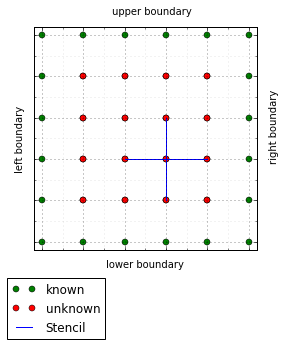
\includegraphics[width=0.5\textwidth]{PoissonEqn/Stencil}
\end{figure}
Unlike the Parabolic equation, the Elliptic equation cannot be estimated by holding one
variable constant and then stepping in that direction. The approximation must be solved at all points at the same instant.\\
\subsection{Matrix representation of the five point scheme}
The five point scheme results in a system of $(N-1)^2$ equations for the $(N-1)^2$ unknowns. This is depicted in Figure \ref{FivePoint} on a $6 \times 6=36$ where there is a grid of $4\times4=16$ unknowns (red) surround by the boundary of $20$ known values.
The general set of $4\times4$ equations of the Poisson difference equation on the $6\times 6$ grid where 
\[h=\frac{1}{6-1}=\frac{1}{5},\]
 can be written as:
\[\begin{array}{l|rcl}
j=1\\
i=1&w_{0,1}+w_{1,0}-4w_{1,1}+w_{1,2}+w_{2,1}&=&\frac{1}{5}^2f_{11}\\
i=2&w_{1,1}+w_{2,0}-4w_{2,1}+w_{2,2}+w_{3,1}&=&\frac{1}{5}^2f_{21}\\
i=3&w_{2,1}+w_{3,0}-4w_{3,1}+w_{3,2}+w_{4,1}&=&\frac{1}{5}^2f_{31}\\
i=4&w_{3,1}+w_{4,0}-4w_{4,1}+w_{4,2}+w_{5,1}&=&\frac{1}{5}^2f_{41}\\
\end{array}
\]	

\[\begin{array}{l|rcl}
j=2\\
i=1&w_{0,2}+w_{1,1}-4w_{1,2}+w_{1,3}+w_{2,2}&=&\frac{1}{5}^2f_{12}\\
i=2&w_{1,2}+w_{2,1}-4w_{2,2}+w_{2,3}+w_{3,2}&=&\frac{1}{5}^2f_{22}\\
i=3&w_{2,2}+w_{3,1}-4w_{3,2}+w_{3,3}+w_{4,2}&=&\frac{1}{5}^2f_{32}\\
i=4&w_{3,2}+w_{4,1}-4w_{4,2}+w_{4,3}+w_{5,2}&=&\frac{1}{5}^2f_{42}\\
\end{array}
\]	

\[\begin{array}{l|rcl}
j=3\\
i=1&w_{0,3}+w_{1,2}-4w_{1,3}+w_{1,4}+w_{2,3}&=&\frac{1}{5}^2f_{13}\\
i=2&w_{1,3}+w_{2,2}-4w_{2,3}+w_{2,4}+w_{3,3}&=&\frac{1}{5}^2f_{23}\\
i=3&w_{2,3}+w_{3,2}-4w_{3,3}+w_{3,4}+w_{4,3}&=&\frac{1}{5}^2f_{33}\\
i=4&w_{3,3}+w_{4,2}-4w_{4,3}+w_{4,4}+w_{5,3}&=&\frac{1}{5}^2f_{43}\\
\end{array}
\]	

\[\begin{array}{l|rcl}
j=4\\
i=1&w_{0,4}+w_{1,3}-4w_{1,4}+w_{1,5}+w_{2,4}&=&\frac{1}{5}^2f_{14}\\
i=2&w_{1,4}+w_{2,3}-4w_{2,4}+w_{2,5}+w_{3,4}&=&\frac{1}{5}^2f_{24}\\
i=3&w_{2,4}+w_{3,3}-4w_{3,4}+w_{3,5}+w_{4,4}&=&\frac{1}{5}^2f_{34}\\
i=4&w_{3,4}+w_{4,3}-4w_{4,4}+w_{4,5}+w_{5,4}&=&\frac{1}{5}^2f_{44}.
\end{array}
\]	
This set of equations can be re-arranged by bringing the known boundary conditions $w_{0,j}$, $w_{5,j}$, $w_{i,0}$ and $w_{i,5}$, to the right hand side.
This can be written as a $16\times 16$ Matrix equation of the  form:\\
\begin{sideways}
\parbox{\textheight}{
\[\left(\begin{array}{cccc|cccc|cccc|cccc}
-4& 1 & 0 &0 &1 &0 &0 &0 &0 &0&0&0&0&0&0&0 \\
1&-4& 1   &0 &0 &1 &0 &0 &0 &0&0&0&0&0&0&0\\
0 &1&-4&1&  0&0 &1 &0 &0 &0&0 &0&0 &0&0&0 \\
0&0 &1&-4&0&  0&0 &1 &0 &0 &0&0 &0&0 &0&0 \\
\hline
1&0&0&0&-4& 1 & 0 &0 &1 &0 &0 &0 &0 &0&0&0 \\
0&1&0&0&1&-4& 1   &0 &0 &1 &0 &0 &0 &0&0&0\\
0&0&1&0&0 &1&-4&1&  0&0 &1 &0 &0 &0&0 &0 \\
0&0&0&1&0&0 &1&-4&0&  0&0 &1 &0 &0 &0&0  \\
\hline
0 &0 &0&0&1&0&0&0&-4& 1 & 0 &0 &1 &0 &0 &0 \\
0 &0 &0&0&0&1&0&0&1&-4& 1   &0 &0 &1 &0 &0\\
0 &0 &0&0&0&0&1&0&0 &1&-4&1&  0&0 &1 &0 \\
0 &0 &0&0&0&0&0&1&0&0 &1&-4&0&  0&0 &1   \\
\hline
0 &0 &0&0&0 &0 &0&0&1&0&0&0&-4& 1 & 0 &0  \\
0 &0 &0&0&0 &0 &0&0&0&1&0&0&1&-4& 1   &0 \\
0 &0 &0&0&0 &0 &0&0&0&0&1&0&0 &1&-4&1 \\
0 &0 &0&0&0 &0 &0&0&0&0&0&1&0&0 &1&-4  \\
\end{array}\right)
\left(\begin{array}{c}
w_{1,1}\\
w_{2,1}\\
w_{3,1}\\
w_{4,1}\\
\hline
w_{1,2}\\
w_{2,2}\\
w_{3,2}\\
w_{4,2}\\
\hline
w_{1,3}\\
w_{2,3}\\
w_{3,3}\\
w_{4,3}\\
\hline
w_{1,4}\\
w_{2,4}\\
w_{3,4}\\
w_{4,4}
\end{array}\right)
=
-\frac{1}{5}^2\left(\begin{array}{c}
f_{1,1}\\
f_{2,1}\\
f_{3,1}\\
f_{4,1}\\
\hline
f_{1,2}\\
f_{2,2}\\
f_{3,2}\\
f_{4,2}\\
\hline
f_{1,3}\\
f_{2,3}\\
f_{3,3}\\
f_{4,3}\\
\hline
f_{1,4}\\
f_{2,4}\\
f_{3,4}\\
f_{4,4}\\
\end{array}\right)
+\left(\begin{array}{c}
-w_{1,0}\\
-w_{2,0}\\
-w_{3,0}\\
-w_{4,0}\\
\hline
0\\
0\\
0\\
0\\
\hline
0\\
0\\
0\\
0\\
\hline
-w_{1,4}\\
-w_{2,4}\\
-w_{3,4}\\
-w_{4,4}\\
\end{array}\right)
+\left(\begin{array}{c}
-w_{0,1}\\
0\\
0\\
-w_{5,1}\\
\hline
-w_{0,2}\\
0\\
0\\
-w_{5,2}\\
\hline
-w_{0,3}\\
0\\
0\\
-w_{5,3}\\
\hline
-w_{0,4}\\
0\\
0\\
-w_{5,4}
\end{array}\right)
\]	
}
\end{sideways}\\
The horizontal and vertical lines are for display purposes to help indicated each set of the four sets of four equations.
\subsection{Generalised Matrix form of the discrete Poisson Equation}
The generalised form of this matrix of the system of equations for the parabolic case results in $(N-1)$ equations, that are written as an $(N-1)^2\times (N-1)^2$ square matrix $A$ and the  $(N-1)^2\times 1$ vectors $\mathbf{w}$, $\mathbf{r}$ and $\mathbf{b}$:
\[ A\mathbf{w}=-h\mathbf{r}+\mathbf{b}.\]
The matrix can be written as following block tridiagonal structure (Figure {SparseMatrix}) :
\begin{eqnarray*}
\left(\begin{array}{ccccccc}
T&I&0&0&.&.&.\\
I&T&I&0&0&.&.\\
0&.&.&.&0&.&.\\
.&.&.&.&.&.&.\\
.&.&.&0&I&T&I\\
.&.&.&.&0&I&T\\
\end{array}\right)
\left(\begin{array}{c}
\mathbf{w}_1\\
\mathbf{w}_2\\
.\\
.\\
\mathbf{w}_{N-2}\\
\mathbf{w}_{N-1}\\
\end{array}\right)
=-h^2
\left(\begin{array}{c}
\mathbf{f}_1\\
\mathbf{f}_2\\
.\\
.\\
\mathbf{f}_{N-2}\\
\mathbf{f}_{N-1}\\
\end{array}\right)
+\left(\begin{array}{c}
\mathbf{b}_1\\
\mathbf{b}_2\\
.\\
.\\
\mathbf{b}_{N-2}\\
\mathbf{b}_{N-1}
\end{array}\right),
\end{eqnarray*}
where $I$ denotes an $(N-1) \times (N-1)$ identity matrix and $T$ is an $(N-1) \times (N-1)$ tridiagonal matrix of the form:
\[ T=\left(\begin{array}{ccccccc}
-4&1&0&0&.&.&.\\
1&-4&1&0&0&.&.\\
0&.&.&.&0&.&.\\
.&.&.&.&.&.&.\\
.&.&.&0&1&-4&1\\
.&.&.&.&0&1&-4\\
\end{array}\right),
\]
$\mathbf{w}_j$ is an $(N-1)\times 1$ vector of approximations $w_{ij}$,
\[\mathbf{w}_j=\left(\begin{array}{c}
w_{1j}\\
w_{2j}\\
.\\
.\\
w_{N-2j}\\
w_{N-1j}\\
\end{array}\right)
\]
the vector $\mathbf{f}$ is made up of $(N-1)$ vectors of length $(N-1)\times 1,$
\[\mathbf{f}_j =\left(\begin{array}{c}
f_{1j}\\
f_{2j}\\
.\\
.\\
f_{N-2j}\\
f_{N-1j}\\
\end{array}\right),
\]
finally $\mathbf{b}$ is the vector of 
boundary conditions made up of two $(N-1)$ vectors of length $(N-1)\times 1$,
\[\mathbf{b}_j =\mathbf{b}_{left,right,j}+\mathbf{b}_{top,bottom,j }=-\left(\begin{array}{c}
g_{0j}\\
0\\
.\\
.\\
0\\
g_{Nj}\\
\end{array}\right)-\left(\begin{array}{c}
0\\
0\\
.\\
.\\
0\\
0\\
\end{array}\right)
\]
for $j=2,..,N-2$, for $j=1$ and $j=N-1$ 
\[
\mathbf{b}_1 =-\left(\begin{array}{c}
g_{10}\\
0\\
.\\
.\\
0\\
g_{1N}\\
\end{array}\right)-\left(\begin{array}{c}
g_{10}\\
g_{20}\\
.\\
.\\
g_{N-20}\\
g_{1N}\\
\end{array}\right), \ \ 
\mathbf{b}_{N-1} =-\left(\begin{array}{c}
g_{0N-1}\\
0\\
.\\
.\\
0\\
g_{NN-1}\\
\end{array}\right)-\left(\begin{array}{c}
g_{1N}\\
g_{2N}\\
.\\
.\\
g_{N-2N}\\
g_{N-1N}\\
\end{array}\right).\]

\begin{figure}[H]
  \caption{Graphical representation of the large sparse matrix $A$ for the discrete solution of the Poisson Equation}\label{SparseMatrix}
  \centering
    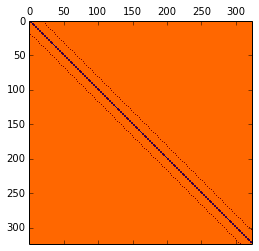
\includegraphics[width=0.5\textwidth]{PoissonEqn/large_matrix}
\end{figure}

The matrix has a unique solution. For sparse matrices of this form an iterative method is used as it would be to computationally expensive to compute the inverse.
\section{Specific Examples}
This section will work through three example problems:
\begin{enumerate}
    \item Homogenous form of the Poisson Equation (Lapalacian),
    \item Poisson Equation with zero boundary conditions,
    \item Poisson Equation with non-zero boundary conditions.
\end{enumerate}
\subsection{Example 1:Homogeneous equation with non-zero boundary}
Consider the Homogeneous Poisson Equation (also known as the Laplacian):\[ \frac{\partial^2 u}{\partial x^2}+\frac{\partial^2 u}{\partial x^2}=0, \ \ \ (x,y) \in \Omega=(0,1)\times (0,1), \]
with boundary conditions:\\
lower boundary,
\[u(x,0) = \sin(2\pi x), \]
upper boundary,
\[u(x,1) = \sin(2\pi x),  \]
left boundary,
\[u(0,y) = 2\sin(2\pi y), \]
right boundary.
\[u(1,y) =  2\sin(2\pi y). \]
The general difference equation for the Laplacian is of the form
\[-(w_{i-1j}+w_{ij-1}-4w_{ij}+w_{ij+1}+w_{i+1j})=0. \]

Here, $N=4$, which gives the step-size,
\[h==\frac{1}{4},\]
and
\[x_i=i\frac{1}{4}, \ \ \ y_j=j\frac{1}{4},\]
for $i=0,1,2,3,4$ and $j=0,1,2,3,4$.
This gives the system of $3\times 3$ equations:
\[\begin{array}{l|rcl}
j=1\\
i=1&w_{0,1}+w_{1,0}-4w_{1,1}+w_{1,2}+w_{2,1}&=&\frac{1}{4}^20\\
i=2&w_{1,1}+w_{2,0}-4w_{2,1}+w_{2,2}+w_{3,1}&=&\frac{1}{4}^20\\
i=3&w_{2,1}+w_{3,0}-4w_{3,1}+w_{3,2}+w_{4,1}&=&\frac{1}{4}^20\\
\end{array}
\]	
\[\begin{array}{l|rcl}
j=2\\
i=1&w_{0,2}+w_{1,1}-4w_{1,2}+w_{1,3}+w_{2,2}&=&\frac{1}{4}^20\\
i=2&w_{1,2}+w_{2,1}-4w_{2,2}+w_{2,3}+w_{3,2}&=&\frac{1}{4}^20\\
i=3&w_{2,2}+w_{3,1}-4w_{3,2}+w_{3,3}+w_{4,2}&=&\frac{1}{4}^20\\
\end{array}
\]	
\[\begin{array}{l|rcl}
j=3\\
i=1&w_{0,3}+w_{1,2}-4w_{1,3}+w_{1,4}+w_{2,3}&=&\frac{1}{4}^20\\
i=2&w_{1,3}+w_{2,2}-4w_{2,3}+w_{2,4}+w_{3,3}&=&\frac{1}{4}^20\\
i=3&w_{2,3}+w_{3,2}-4w_{3,3}+w_{3,4}+w_{4,3}&=&\frac{1}{4}^20.
\end{array}
\]	

This system is then rearranged by bringing the known boundary conditions to the right hand side, to give:
\[\begin{array}{l|rcl}
j=1\\
i=1&-4w_{1,1}+w_{1,2}+w_{2,1}&=&\frac{1}{4}^20-w_{0,1}-w_{1,0}\\
i=2&w_{1,1}-4w_{2,1}+w_{2,2}+w_{3,1}&=&\frac{1}{4}^20-w_{2,0}\\
i=3&w_{2,1}-4w_{3,1}+w_{3,2}&=&\frac{1}{4}^20-w_{4,1}-w_{3,0}\\
\end{array}
\]	
\[\begin{array}{l|rcl}
j=2\\
i=1&w_{1,1}-4w_{1,2}+w_{1,3}+w_{2,2}&=&\frac{1}{4}^20-w_{0,2}\\
i=2&w_{1,2}+w_{2,1}-4w_{2,2}+w_{2,3}+w_{3,2}&=&\frac{1}{4}^20\\
i=3&w_{2,2}+w_{3,1}-4w_{3,2}+w_{3,3}&=&\frac{1}{4}^20-w_{4,2}\\
\end{array}
\]	
\[\begin{array}{l|rcl}
j=3\\
i=1&w_{1,2}-4w_{1,3}+w_{2,3}&=&\frac{1}{4}^20-w_{0,3}-w_{1,4}\\
i=2&w_{1,3}+w_{2,2}-4w_{2,3}+w_{3,3}&=&\frac{1}{4}^20-w_{2,4}\\
i=3&w_{2,3}+w_{3,2}-4w_{3,3}&=&\frac{1}{4}^20-w_{4,3}-w_{3,4}\\
\end{array}
\]	
Given the discrete boundary conditions:
\[
\begin{array}{lcl}
\textbf{Left boundary}&\ \ \ & \textbf{Right boundary}\\ 
x_0=0&\ \ \ & x_4=1\\ 
u(0,y)=2\sin(2\pi y)&\ \ \ & u(1,y)=2\sin(2\pi y)\\

w_{0,0}=0 &\ \ \ & w_{4,0}=0\\ 
w_{0,1}=2\sin(2\pi y_1) =2 & \ \ \ & w_{4,1}=2\sin(2\pi y_1) =2\\

w_{0,2}=2\sin(2\pi y_2) =0 & \ \ \ & w_{4,2}=2\sin(2\pi y_2) =0\\

w_{0,3}=2\sin(2\pi y_3) =-2 & \ \ \ & w_{4,3}=2\sin(2\pi y_3) =-2\\

w_{0,4}=2\sin(2\pi y_4) =0 & \ \ \ & w_{4,4}=2\sin(2\pi y_4) =0\\

\end{array}
\]
\[
\begin{array}{lcl}
\textbf{Lower boundary}&\ \ \ & \textbf{Upper boundary}\\ 
 y_0=0&\ \ \ & y_4=1 \\
 u(x,0)=\sin(2\pi x)&\ \ \ & u(x,1)=\sin(2\pi x) \\

 w_{0,0}=0 & \ \ \ & w_{0,4}=0\\ 

w_{1,0}=\sin(2\pi x_1) =1  & \ \ \ & w_{1,4}=\sin(2\pi x_1) =1 \\


w_{2,0}=\sin(2\pi x_2) =0  & \ \ \ & w_{2,4}=\sin(2\pi x_2) =0 \\


w_{3,0}=\sin(2\pi x_3) =-1  & \ \ \ & w_{3,4}=\sin(2\pi x_3) =-1 \\


w_{4,0}=\sin(2\pi x_4) =0  & \ \ \ & w_{4,4}=\sin(2\pi x_4) =0 \\

\end{array}
\]

The system of equations are written in matrix form:
\[\left(\begin{array}{ccccccccc}
-4& 1 & 0 &1 &0 &0 &0 &0 &0\\
1&-4& 1 & 0 &1 &0 &0 &0 &0 \\
0 &1&-4&  0&0 &1 &0 &0 &0 \\
1 &0 &0 &-4& 1 & 0 &1 &0 &0\\
0 & 1 &0 &1&-4& 1 &0 &1 &0  \\
0 &0 &1 &0 &1&-4&0&  0 &1  \\
0&0&0&1 &0 &0 &-4& 1 & 0\\
0&0&0&0 & 1 &0 &1&-4& 1   \\
0&0&0&0 &0 &1 &0 &1&-4
\end{array}\right)
\left(\begin{array}{c}
w_{1,1}\\
w_{2,1}\\
w_{3,1}\\
w_{1,2}\\
w_{2,2}\\
w_{3,2}\\
w_{1,3}\\
w_{2,3}\\
w_{3,3}
\end{array}\right)=
\left(\begin{array}{c}
-w_{1,0}\\
-w_{2,0}\\
-w_{3,0}\\
0\\
0\\
0\\
-w_{1,4}\\
-w_{2,4}\\
-w_{3,4}
\end{array}\right)
+\left(\begin{array}{c}
-w_{0,1}\\
0\\
-w_{4,1}\\
-w_{0,2}\\
0\\
-w_{4,2}\\
-w_{0,3}\\
0\\
-w_{4,3}
\end{array}\right),
\]	
where the matrix is $3^2\times 3^2$ which is graphically represented in Figure \ref{9x9 Matrix}, where the colours indicated the values in each cell.
\begin{figure}[H]
  \caption{Graphical representation of the matrix}\label{9x9 Matrix}
  \centering
    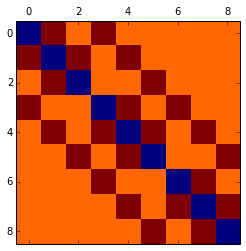
\includegraphics[width=0.5\textwidth]{PoissonEqn/matrix}
\end{figure}

For the given boundary conditions the matrix equation is written as :
\[\left(\begin{array}{ccccccccc}
-4& 1 & 0 &1 &0 &0 &0 &0 &0\\
1&-4& 1 & 0 &1 &0 &0 &0 &0 \\
0 &1&-4&  0&0 &1 &0 &0 &0 \\
1 &0 &0 &-4& 1 & 0 &1 &0 &0\\
0 & 1 &0 &1&-4& 1 &0 &1 &0  \\
0 &0 &1 &0 &1&-4&0&  0 &1  \\
0&0&0&1 &0 &0 &-4& 1 & 0\\
0&0&0&0 & 1 &0 &1&-4& 1   \\
0&0&0&0 &0 &1 &0 &1&-4
\end{array}\right)
\left(\begin{array}{c}
w_{1,1}\\
w_{2,1}\\
w_{3,1}\\
w_{1,2}\\
w_{2,2}\\
w_{3,2}\\
w_{1,3}\\
w_{2,3}\\
w_{3,3}
\end{array}\right)=
\left(\begin{array}{c}
-1\\
0\\
1\\
0\\
0\\
0\\
-1\\
0\\
1
\end{array}\right)
+\left(\begin{array}{c}
-2\\
0\\
-2\\
0\\
0\\
0\\
2\\
0\\
2
\end{array}\right).
\]	
Figure \ref{SolPossLap} shows the approximate solution of the Laplacian Equation for the given boundary conditions and $h=\frac{1}{4}$.
\begin{figure}[H]
  \caption{Numerical solution of the homogeneous differential equation }\label{SolPossLap}
  \centering
    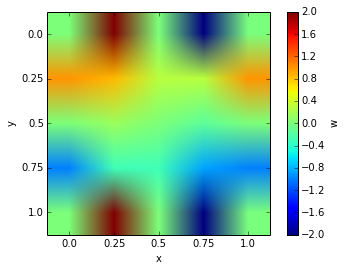
\includegraphics{PoissonEqn/solution_homogeneous}
\end{figure}

\subsection{Example 2: non-homogeneous equation with zero boundary}
Consider the Poission Equation
\[ \frac{\partial^2 u}{\partial x^2}+\frac{\partial^2 u}{\partial x^2}=x^2+y^2 \ \ \ (x,y) \in \Omega=(0,1)\times (0,1) \]
with zero boundary conditions:
Left boundary:
\[u(x,0) =0 \]
Right boundary:
\[u(x,1) = 0  \]
Lower boundary:
\[u(0,y) = 0 \]
Upper boundary:
\[u(1,y) =  0. \]
The difference equation is of the form:
\[-(w_{i-1j}+w_{ij-1}-4w_{ij}+w_{ij+1}+w_{i+1j})=h^2(x_i^2+y_j^2). \]
Here, $N=4$, which gives the step-size,
\[h==\frac{1}{4},\]
and
\[x_i=i\frac{1}{4}, \ \ \ y_j=j\frac{1}{4},\]
for $i=0,1,2,3,4$ and $j=0,1,2,3,4$.
This gives the system of $3\times 3$ equations:
\[\begin{array}{l|rcl}
j=1\\
i=1&w_{0,1}+w_{1,0}-4w_{1,1}+w_{1,2}+w_{2,1}&=&\frac{1}{4}^2(x_1^2+y_1^2)\\
i=2&w_{1,1}+w_{2,0}-4w_{2,1}+w_{2,2}+w_{3,1}&=&\frac{1}{4}^2(x_2^2+y_1^2)\\
i=3&w_{2,1}+w_{3,0}-4w_{3,1}+w_{3,2}+w_{4,1}&=&\frac{1}{4}^2(x_3^2+y_1^2)\\
\end{array}
\]	
\[\begin{array}{l|rcl}
j=2\\
i=1&w_{0,2}+w_{1,1}-4w_{1,2}+w_{1,3}+w_{2,2}&=&\frac{1}{4}^2(x_1^2+y_2^2)\\
i=2&w_{1,2}+w_{2,1}-4w_{2,2}+w_{2,3}+w_{3,2}&=&\frac{1}{4}^2(x_2^2+y_2^2)\\
i=3&w_{2,2}+w_{3,1}-4w_{3,2}+w_{3,3}+w_{4,2}&=&\frac{1}{4}^2(x_3^2+y_2^2)\\
\end{array}
\]	
\[\begin{array}{l|rcl}
j=3\\
i=1&w_{0,3}+w_{1,2}-4w_{1,3}+w_{1,4}+w_{2,3}&=&\frac{1}{4}^2(x_1^2+y_3^2)\\
i=2&w_{1,3}+w_{2,2}-4w_{2,3}+w_{2,4}+w_{3,3}&=&\frac{1}{4}^2(x_2^2+y_3^2)\\
i=3&w_{2,3}+w_{3,2}-4w_{3,3}+w_{3,4}+w_{4,3}&=&\frac{1}{4}^2(x_3^2+y_3^2)\\
\end{array}
\]	
This  system  is  then  rearranged  by  bringing  the  known  boundary conditions to the right hand side, to give:
\[\begin{array}{l|rcl}

j=1\\
i=1&-4w_{1,1}+w_{1,2}+w_{2,1}&=&\frac{1}{4}^2(x_1^2+y_1^2)-w_{0,1}-w_{1,0}\\
i=2&w_{1,1}-4w_{2,1}+w_{2,2}+w_{3,1}&=&\frac{1}{4}^2(x_2^2+y_1^2)-w_{2,0}\\
i=3&w_{2,1}-4w_{3,1}+w_{3,2}&=&\frac{1}{4}^2(x_3^2+y_1^2)-w_{4,1}-w_{3,0}\\
\end{array}
\]	
\[\begin{array}{l|rcl}
j=2\\
i=1&w_{1,1}-4w_{1,2}+w_{1,3}+w_{2,2}&=&\frac{1}{4}^2(x_1^2+y_2^2)-w_{0,2}\\
i=2&w_{1,2}+w_{2,1}-4w_{2,2}+w_{2,3}+w_{3,2}&=&\frac{1}{4}^2(x_2^2+y_2^2)\\
i=3&w_{2,2}+w_{3,1}-4w_{3,2}+w_{3,3}&=&\frac{1}{4}^2(x_3^2+y_2^2)-w_{4,2}\\
\end{array}
\]	
\[\begin{array}{l|rcl}
j=3\\
i=1&w_{1,2}-4w_{1,3}+w_{2,3}&=&\frac{1}{4}^2(x_1^2+y_3^2)-w_{0,3}-w_{1,4}\\
i=2&w_{1,3}+w_{2,2}-4w_{2,3}+w_{3,3}&=&\frac{1}{4}^2(x_2^2+y_3^2)-w_{2,4}\\
i=3&w_{2,3}+w_{3,2}-4w_{3,3}&=&\frac{1}{4}^2(x_3^2+y_3^2)-w_{4,3}-w_{3,4}.\\
\end{array}
\]	
Given the zero boundary conditions
\[
\begin{array}{lcl}
\textbf{Lower Boundary}&\ \ \ & \textbf{Upper Boundary} \\
x_0=0&\ \ \ & x_4=1\\
u(0,y)=0&\ \ \ & u(1,y)=0\\
w_{0,0}=0 &\ \ \ & w_{4,0}=0 \\ 
w_{0,1}=0& \ \ \ & w_{4,1}=0 \\
w_{0,2}=0 & \ \ \ & w_{4,2}=0  \\
w_{0,3}=0& \ \ \ & w_{4,3}=0  \\
w_{0,4}=0 & \ \ \ & w_{4,4}=0  \\

\end{array}
\]
\[
\begin{array}{lcl}
\textbf{Left Boundary}&\ \ \ & \textbf{Right Boundary} \\
y_0=0&\ \ \ & y_4=1 \\
u(x,0)=0&\ \ \ & u(x,1)=0 \\

w_{0,0}=0 & \ \ \ & w_{0,4}=0\\ 
w_{1,0}=0  & \ \ \ & w_{1,4}=0 \\
w_{2,0}=0  & \ \ \ & w_{2,4}=0 \\
w_{3,0}=0  & \ \ \ & w_{3,4}=0 \\
w_{4,0}=0  & \ \ \ & w_{4,4}=0 \\

\end{array}
\]

The system of equations can be written in matrix form:
\[\left(\begin{array}{ccccccccc}
-4& 1 & 0 &1 &0 &0 &0 &0 &0\\
1&-4& 1 & 0 &1 &0 &0 &0 &0 \\
0 &1&-4&  0&0 &1 &0 &0 &0 \\
1 &0 &0 &-4& 1 & 0 &1 &0 &0\\
0 & 1 &0 &1&-4& 1 &0 &1 &0  \\
0 &0 &1 &0 &1&-4&0&  0 &1  \\
0&0&0&1 &0 &0 &-4& 1 & 0\\
0&0&0&0 & 1 &0 &1&-4& 1   \\
0&0&0&0 &0 &1 &0 &1&-4
\end{array}\right)
\left(\begin{array}{c}
w_{1,1}\\
w_{2,1}\\
w_{3,1}\\
w_{1,2}\\
w_{2,2}\\
w_{3,2}\\
w_{1,3}\\
w_{2,3}\\
w_{3,3}
\end{array}\right)=
h^2\left(\begin{array}{c}
(x_1^2+y_1^2)\\
(x_2^2+y_1^2)\\
(x_3^2+y_1^2)\\
(x_1^2+y_2^2)\\
(x_2^2+y_2^2)\\
(x_3^2+y_2^2)\\
(x_1^2+y_3^2)\\
(x_2^2+y_3^2)\\
(x_3^2+y_3^2)
\end{array}\right).
\]	
Substituting values into the right hand side gives the specific matric form:
\[\left(\begin{array}{ccccccccc}
-4& 1 & 0 &1 &0 &0 &0 &0 &0\\
1&-4& 1 & 0 &1 &0 &0 &0 &0 \\
0 &1&-4&  0&0 &1 &0 &0 &0 \\
1 &0 &0 &-4& 1 & 0 &1 &0 &0\\
0 & 1 &0 &1&-4& 1 &0 &1 &0  \\
0 &0 &1 &0 &1&-4&0&  0 &1  \\
0&0&0&1 &0 &0 &-4& 1 & 0\\
0&0&0&0 & 1 &0 &1&-4& 1   \\
0&0&0&0 &0 &1 &0 &1&-4
\end{array}\right)
\left(\begin{array}{c}
w_{1,1}\\
w_{2,1}\\
w_{3,1}\\
w_{1,2}\\
w_{2,2}\\
w_{3,2}\\
w_{1,3}\\
w_{2,3}\\
w_{3,3}
\end{array}\right)=
\left(\begin{array}{c}
0.0078125\\
0.01953125\\
0.0390625 \\
 0.01953125\\
 0.0312\\
0.05078125\\
0.0390625\\
0.05078125\\
0.0703125
\end{array}\right).
\]	
Figure \ref{SolPossZero} shows the numerical solution of the Poisson Equation with zero boundary conditions.
\begin{figure}[H]
  \caption{Numerical solution of the differential equation with 0 boundary conditions }\label{SolPossZero}
  \centering
    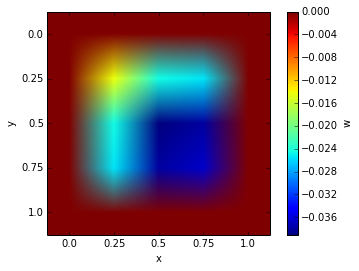
\includegraphics{PoissonEqn/solution_zero_boundary}
\end{figure}

\subsection{Example 3: Inhomogeneous equation with non-zero boundary}
Consider the Poisson Equation 
\[ \frac{\partial^2 u}{\partial x^2}+\frac{\partial^2 u}{\partial x^2}=xy, \ \ \ (x,y) \in \Omega=(0,1)\times (0,1), \]
with boundary conditions\\
Right Boundary
\[u(x,0) =-x^2+x \]
Left Boundary
\[u(x,1) = x^2-x  \]
Lower Boundary
\[u(0,y) = -y^2+y \]
Upper Boundary
\[u(1,y) =  -y^2+y. \]
The five point difference equation is of the form 
\[-(w_{i-1j}+w_{ij-1}-4w_{ij}+w_{ij+1}+w_{i+1j})=h^2(x_iy_j). \]
Here, $N=4$, which gives the step-size,
\[h==\frac{1}{4},\]
and
\[x_i=i\frac{1}{4}, \ \ \ y_j=j\frac{1}{4},\]
for $i=0,1,2,3,4$ and $j=0,1,2,3,4$.
This gives the system of $3\times 3$ equations:
\[\begin{array}{l|rcl}
i=1&w_{0,1}+w_{1,0}-4w_{1,1}+w_{1,2}+w_{2,1}&=&\frac{1}{4}^2(x_1y_1)\\
i=2&w_{1,1}+w_{2,0}-4w_{2,1}+w_{2,2}+w_{3,1}&=&\frac{1}{4}^2(x_2y_1)\\
i=3&w_{2,1}+w_{3,0}-4w_{3,1}+w_{3,2}+w_{4,1}&=&\frac{1}{4}^2(x_3y_1)\\
\end{array}\]	
\[\begin{array}{l|rcl}
j=2\\
i=1&w_{0,2}+w_{1,1}-4w_{1,2}+w_{1,3}+w_{2,2}&=&\frac{1}{4}^2(x_1y_2)\\
i=2&w_{1,2}+w_{2,1}-4w_{2,2}+w_{2,3}+w_{3,2}&=&\frac{1}{4}^2(x_2y_2)\\
i=3&w_{2,2}+w_{3,1}-4w_{3,2}+w_{3,3}+w_{4,2}&=&\frac{1}{4}^2(x_3y_2)\\
\end{array}\]	
\[\begin{array}{l|rcl}
j=3\\
i=1&w_{0,3}+w_{1,2}-4w_{1,3}+w_{1,4}+w_{2,3}&=&\frac{1}{4}^2(x_1y_3)\\
i=2&w_{1,3}+w_{2,2}-4w_{2,3}+w_{2,4}+w_{3,3}&=&\frac{1}{4}^2(x_2y_3)\\
i=3&w_{2,3}+w_{3,2}-4w_{3,3}+w_{3,4}+w_{4,3}&=&\frac{1}{4}^2(x_3y_3).
\end{array}
\]	
Re-arranging the system such that the known values are on the right hand side:
\[\begin{array}{l|rcl}
j=1\\
i=1&-4w_{1,1}+w_{1,2}+w_{2,1}&=&\frac{1}{4}^2(x_1y_1)-w_{0,1}-w_{1,0}\\
i=2&w_{1,1}-4w_{2,1}+w_{2,2}+w_{3,1}&=&\frac{1}{4}^2(x_2y_1)-w_{2,0}\\
i=3&w_{2,1}-4w_{3,1}+w_{3,2}&=&\frac{1}{4}^2(x_3y_1)-w_{4,1}-w_{3,0}\\
\end{array}\]	
\[\begin{array}{l|rcl}
j=2\\
i=1&w_{1,1}-4w_{1,2}+w_{1,3}+w_{2,2}&=&\frac{1}{4}^2(x_1y_2)-w_{0,2}\\
i=2&w_{1,2}+w_{2,1}-4w_{2,2}+w_{2,3}+w_{3,2}&=&\frac{1}{4}^2(x_2y_2)\\
i=3&w_{2,2}+w_{3,1}-4w_{3,2}+w_{3,3}&=&\frac{1}{4}^2(x_3y_2)-w_{4,2}\\
\end{array}\]	
\[\begin{array}{l|rcl}
j=3\\
i=1&w_{1,2}-4w_{1,3}+w_{2,3}&=&\frac{1}{4}^2(x_1y_3)-w_{0,3}-w_{1,4}\\
i=2&w_{1,3}+w_{2,2}-4w_{2,3}+w_{3,3}&=&\frac{1}{4}^2(x_2y_3)-w_{2,4}\\
i=3&w_{2,3}+w_{3,2}-4w_{3,3}&=&\frac{1}{4}^2(x_3y_3)-w_{4,3}-w_{3,4}.
\end{array}
\]	

The discrete boundary conditions are
\[
\begin{array}{lcl}
\textbf{Left boundary}&\ \ \ & \textbf{Right boundary}\\ 
x_0=0&\ \ \ & x_4=1\\ 
u(0,y)=-y^2+y&\ \ \ & u(1,y)=-y^2+y\\

w_{0,0}=0 &\ \ \ & w_{4,0}=0\\ 
w_{0,1}=-y^2_1+y_1 =\frac{3}{16} & \ \ \ & w_{4,1}=-y^2_1+y_1 =\frac{1}{16}\\

w_{0,2}=-y^2_2+y_2 =\frac{1}{4} & \ \ \ & w_{4,2}=-y^2_2+y_2 =\frac{1}{4}\\

w_{0,3}=-y^2_3+y_3 =\frac{3}{16} & \ \ \ & w_{4,3}=-y^2_3+y_3 =\frac{3}{16}\\

w_{0,4}=-y^2_4+y_4 =0 & \ \ \ & w_{4,4}=-y^2_4+y_4 =0\\

\end{array}
\]
\[
\begin{array}{lcl}
\textbf{Lower boundary}&\ \ \ & \textbf{Upper boundary}\\ 
 y_0=0&\ \ \ & y_4=1 \\
 u(x,0)=-x^2+x&\ \ \ & u(x,1)=x^2-x \\

 w_{0,0}=0 & \ \ \ & w_{0,4}=0\\ 

w_{1,0}=-x^2_1+x_1 =\frac{3}{16}  & \ \ \ & w_{1,4}=x^2_1-x_1 =-\frac{3}{16} \\


w_{2,0}=-x^2_2+x_2 =\frac{1}{4}  & \ \ \ & w_{2,4}=x^2_2-x_2 =-\frac{1}{4} \\


w_{3,0}=-x^2_3+x_3 =\frac{3}{16}  & \ \ \ & w_{3,4}=x^2_3-x_3 =-\frac{3}{16} \\


w_{4,0}=0  & \ \ \ & w_{4,4}=0 \\

\end{array}
\]
The system of equations can be written 
in $9\times 9$ Matrix form:
\[\left(\begin{array}{ccccccccc}
-4& 1 & 0 &1 &0 &0 &0 &0 &0\\
1&-4& 1 & 0 &1 &0 &0 &0 &0 \\
0 &1&-4&  0&0 &1 &0 &0 &0 \\
1 &0 &0 &-4& 1 & 0 &1 &0 &0\\
0 & 1 &0 &1&-4& 1 &0 &1 &0  \\
0 &0 &1 &0 &1&-4&0&  0 &1  \\
0&0&0&1 &0 &0 &-4& 1 & 0\\
0&0&0&0 & 1 &0 &1&-4& 1   \\
0&0&0&0 &0 &1 &0 &1&-4
\end{array}\right)
\left(\begin{array}{c}
w_{1,1}\\
w_{2,1}\\
w_{3,1}\\
w_{1,2}\\
w_{2,2}\\
w_{3,2}\\
w_{1,3}\\
w_{2,3}\\
w_{3,3}
\end{array}\right)=\]
\[
h^2\left(\begin{array}{c}
(x_1y_1)\\
(x_2y_1)\\
(x_3y_1)\\
(x_1y_2)\\
(x_2y_2)\\
(x_3y_2)\\
(x_1y_3)\\
(x_2y_3)\\
(x_3y_3)
\end{array}\right)+
\left(\begin{array}{c}
-w_{1,0}\\
-w_{2,0}\\
-w_{3,0}\\
0\\
0\\
0\\
-w_{1,4}\\
-w_{2,4}\\
-w_{3,4}
\end{array}\right)
+\left(\begin{array}{c}
-w_{0,1}\\
0\\
-w_{4,1}\\
-w_{0,2}\\
0\\
-w_{4,2}\\
-w_{0,3}\\
0\\
-w_{4,3}
\end{array}\right),
\]	
inputting the specific boundary values and the right hand side of the equation gives:
\[\left(\begin{array}{ccccccccc}
-4& 1 & 0 &1 &0 &0 &0 &0 &0\\
1&-4& 1 & 0 &1 &0 &0 &0 &0 \\
0 &1&-4&  0&0 &1 &0 &0 &0 \\
1 &0 &0 &-4& 1 & 0 &1 &0 &0\\
0 & 1 &0 &1&-4& 1 &0 &1 &0  \\
0 &0 &1 &0 &1&-4&0&  0 &1  \\
0&0&0&1 &0 &0 &-4& 1 & 0\\
0&0&0&0 & 1 &0 &1&-4& 1   \\
0&0&0&0 &0 &1 &0 &1&-4
\end{array}\right)
\left(\begin{array}{c}
w_{1,1}\\
w_{2,1}\\
w_{3,1}\\
w_{1,2}\\
w_{2,2}\\
w_{3,2}\\
w_{1,3}\\
w_{2,3}\\
w_{3,3}
\end{array}\right)=\]
\[
\left(\frac{1}{4}\right)^2\left(\begin{array}{c}
0.0625\\
0.125\\
0.1875 \\
0.125\\
 0.25\\
0.375\\
0.1875\\
0.375\\
0.5626
\end{array}\right)
+\left(\begin{array}{c}
-\frac{3}{16}\\
-\frac{1}{4}\\
-\frac{3}{16}\\
0\\
0\\
0\\
\frac{3}{16}\\
\frac{1}{4}\\
\frac{3}{16}
\end{array}\right)
+\left(\begin{array}{c}
-\frac{3}{16}\\
0\\
-\frac{3}{16}\\
-\frac{1}{4}\\
0\\
-\frac{1}{4}\\
-\frac{3}{16}\\
0\\
-\frac{3}{16}
\end{array}\right).
\]	
Figure \ref{SolPoss} shows the numerical solution of the Poisson Equation with non-zero boundary conditions.
\begin{figure}[H]
  \caption{Numerical solution of the differential equation with non-zero boundary conditions }\label{SolPoss}
  \centering
    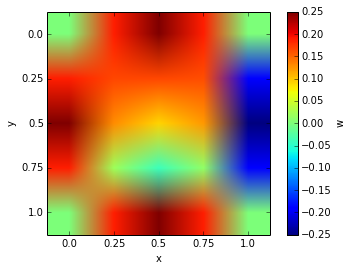
\includegraphics{PoissonEqn/Solution_full_equation}
\end{figure}

\section{Consistency and Convergence}
We now ask how well the grid function determined by the five point scheme approximates
the exact solution of the Poisson problem.
\begin{definition}
Let $L_h$ denote the finite difference approximation associated with the grid $\Omega_h$ having the mesh size $h$, to a partial differential operator $L$ defined on
a simply connected, open set $\Omega \subset R^2$. For a given function $\varphi\in C^{\infty}(\Omega)$,
the truncation error of $L_h$ is
\[\tau_{h}(\mathbf{x})=(L-L_h)\varphi(x) \]
The approximation $L_h$ is consistent with $L$ if
\[ \lim_{h\rightarrow 0}\tau_h(x)=0,\]
for all $\mathbf{x} \in D$ and all $\varphi \in C^{\infty}(\Omega)$. The approximation is consistent to order $p$ if $\tau_h(\mathbf{x})=O(h^p)$.
$\circ$
\end{definition}
While we have seen this definition a few times it is always interesting how the
terms are denoted and expressed but the ideas are always the same.
\begin{proposition}
The five-point difference analog $-\nabla^2_h$ is consistent to order 2 with $-\nabla^2$.
\end{proposition}
\begin{proof}
Pick $\varphi \in C^{\infty}(D)$, and let $(x,y) \in \Omega$ be a point such that $(x\pm h, y),(x,y \pm h) \in \Omega\bigcup \partial\Omega$.  By the Taylor Theorem
\begin{eqnarray*}
\varphi(x\pm h,y)&=&\varphi(x,y) \pm h \frac{\partial \varphi}{\partial x}(x,y)+\frac{h^2}{2!}\frac{\partial^2 \varphi}{\partial x^2}(x,y) \pm\frac{h^3}{3!}\frac{\partial^3 \varphi}{\partial x^3}(x,y)+\frac{h^4}{4!}\frac{\partial^4 \varphi}{\partial x^4}(\zeta^{\pm},y)
\end{eqnarray*}
where $\zeta^{\pm} \in (x-h,x+h)$. Adding this pair of equation together and rearranging , we get
\[\frac{1}{h^2}[\varphi(x+h,y)-2\varphi(x,y)+\varphi(x-h,y) ] -\frac{\partial^2 \varphi}{\partial x^2}(x,y)=\frac{h^2}{4!}\left[\frac{\partial^4 \varphi}{\partial x^4}(\zeta^{+},y)+
\frac{\partial^4 \varphi}{\partial x^4}(\zeta^{-},y)
 \right]
\]
By the intermediate value theorem
\[\left[\frac{\partial^4 \varphi}{\partial x^4}(\zeta^{+},y)+
\frac{\partial^4 \varphi}{\partial x^4}(\zeta^{-},y)
 \right]
=2\frac{\partial^4 \varphi}{\partial x^4}(\zeta,y),\]
for some $\zeta \in (x-h,x+h)$.  Therefore,
\[\delta_x^2(x,y)
=\frac{\partial^2 \varphi}{\partial x^2}(x,y)+\frac{h^2}{2!}\frac{\partial^4 \varphi}{\partial x^4}(\zeta,y)
\]
Similar reasoning shows that
\[\delta_y^2(x,y)
=\frac{\partial^2 \varphi}{\partial y^2}(x,y)+\frac{h^2}{2!}\frac{\partial^4 \varphi}{\partial y^4}(x,\eta)
\]
for some $\eta \in (y-h,y+h)$. We conclude that $\tau_h(x,y)=(\nabla-\nabla_h)\varphi(x,y)=O(h^2).$
$\bullet$\end{proof}
Consistency does not guarantee that the solution to the difference equations approximates the exact solution to the \addtoindex{PDE}. 
\begin{definition}
Let $L_hw(\mathbf{x}_j)=f(\mathbf{x}_j)$ be a finite difference approximation, defined on a grid mesh size h, to a \addtoindex{PDE} $LU(\mathbf{x})=f(\mathbf{x})$ on a simply
connected set $D \subset R^n$. Assume that $w(x,y)=U(x,y)$ at all points (x,y) on the boundary $\partial\Omega$.  The finite difference scheme converges (or is convergent) if
\[ \max_j|U(\mathbf{x}_j)-w(\mathbf{x}_j)| \rightarrow 0 \mbox{  as  } h \rightarrow 0.\]
$\circ$
\end{definition}
For the five point scheme there is a direct connection between consistency and convergence.  Underlying this connection is an argument based on the following principle:
\begin{theorem}
(DISCRETE MAXIMUM PRINCIPLE).
If $\nabla^2_hV_{ij}\geq 0$ for all points $(x_i,y_j) \in \Omega_h$, then
\[ \max_{(x_i,y_j)\in\Omega_h}V_{ij}\leq  \max_{(x_i,y_j)\in\partial\Omega_h}V_{ij}\]
If $\nabla^2_hV_{ij}\leq 0$ for all points $(x_i,y_j) \in \Omega_h$, then
\[ \min_{(x_i,y_j)\in\Omega_h}V_{ij}\geq  \min_{(x_i,y_j)\in\partial\Omega_h}V_{ij}\]
\end{theorem}
In other words, a grid function $V$ for which $\nabla^2_hV$ is nonnegative on $\Omega_h$ attains its maximum on the boundary $\partial\Omega_h$ of the grid.  Similarly, if $\nabla^2_hV$ is nonpositive on $\Omega_h$, then V attains its minimum on the boundary $\partial\Omega_h$.
\begin{proof}
The proof is by contradiction.  We argue for the case $\nabla_h^2V_{ij} \geq 0$, reasoning for the case $\nabla_h^2V_{ij}\leq 0$ begin similar.\\
Assume that $V$ attains its maximum value M at an interior grid point $(x_I,y_J)$ and that $\max_{(x_i,y_j)\in\partial\Omega_h}V_{ij}<M.$ The hypothesis $\nabla_{h}^2V_{ij} \geq 0$ implies that
\[ V_{IJ}\leq\frac{1}{4}(V_{I+1J}+V_{I-1J}+V_{IJ+1}+V_{IJ-1}) \]
This cannot hold unless
\[ V_{I+1J}=V_{I-1J}=V_{IJ+1}=V_{IJ-1}=M. \]
If any of the corresponding grid points $(x_{I+1},y_{L}),(x_{J-1},y_{L}),(x_{I},y_{L+1}),(x_{I},y_{L-1})$ lies in $\partial\Omega_h$, then we have reached the 
desired contradiction.\\
Otherwise, we continue arguing in this way until we conclude that $V_{I+iJ+j}=M$
for some point $(x_{I+iJ+j})\in \partial\Omega$, which again gives a contradiction.
$\bullet$\end{proof}
This leads to interesting results
\begin{proposition}
\begin{enumerate}
\item
The zero grid function (for which $U_{ij}=0$ for all $(x_i,y_j) \in \Omega_h \bigcup \partial\Omega_h$
is the only solution to the finite difference problem
\[\nabla_h^2U_{ij}=0 \mbox{ for }(x_i,y_j)\in\Omega_h,\]
\[U_{ij}=0 \mbox{ for }(x_i,y_j)\in\partial\Omega_h.\]
\item
For prescribed grid functions $f_{ij}$ and $g_{ij}$, there exists a unique solution to the problem
\[\nabla_h^2U_{ij}=f_{ij} \mbox{ for }(x_i,y_j)\in\Omega_h,\]
\[U_{ij}=g_{ij} \mbox{ for }(x_i,y_j)\in\partial\Omega_h.\]
\end{enumerate}
\end{proposition}
\begin{definition}
For any grid function $V:\Omega_h\bigcup\partial\Omega_h \rightarrow R$,
\[||V||_{\Omega} =\max_{(x_i,y_j)\in\Omega_h}|V_{ij}|, \]
\[||V||_{\partial\Omega} =\max_{(x_i,y_j)\in\partial\Omega_h}|V_{ij}|. \]
$\circ$
\end{definition}
\begin{lemma}
If the grid function $V:\Omega_h\bigcup\partial\Omega_h\rightarrow R$ satisfies the boundary condition $V_{ij}=0$ for $(x_i,y_j)\in \partial\Omega_h$, then
\[||V_||_{\Omega}\leq \frac{1}{8}||\nabla_h^2V||_{\Omega} \]
\end{lemma}
\begin{proof}
Let $\nu = ||\nabla_{h}^2V||_{\Omega}$. Clearly for all points $(x_i,y_j)\in\Omega_h$,
\begin{equation}\label{ineq 828}
-\nu \leq \nabla_{h}^2V_{ij} \leq \nu \end{equation}
Now we define $W:\Omega_h \bigcup \partial\Omega_h \rightarrow R$ by setting 
$W_{ij}=\frac{1}{4}[(x_i-\frac{1}{2})^2+(y_j-\frac{1}{2})^2]$, which is nonnegative.  Also $\nabla_h^2W_{ij}=1$ and that $||W||_{\partial\Omega}=\frac{1}{8}$.
The inequality (\ref{ineq 828}) implies that, for all points $(x_i,y_j)\in\Omega_h$,
\[\nabla_h^2(V_{ij}+\nu W_{ij})\geq 0 \]
\[\nabla_h^2(V_{ij}-\nu W_{ij})\leq 0 \]
By the discrete minimum principle and the fact that V vanishes on $\partial\Omega_h$
\[V_{ij}\leq V_{ij}+\nu W_{ij}\leq \nu||W||_{\partial\Omega} \]
\[V_{ij}\geq V_{ij}-\nu W_{ij}\geq -\nu||W||_{\partial\Omega} \]
Since $||W||_{\partial\Omega}=\frac{1}{8}$
\[||V_||_{\Omega}\leq \frac{1}{8}\nu =\frac{1}{8}||\nabla_h^2V||_{\Omega} \]
$\bullet$\end{proof}
Finally we prove that the five point scheme for the \addtoindex{Poisson equation} is convergent.
\begin{theorem}
Let $U$ be a solution to the \addtoindex{Poisson equation} and let $w$ be the grid function
that satisfies the discrete analog
\[-\nabla_h^2w_{ij}=f_{ij} \ \ \mbox{ for } (x_i,y_j)\in\Omega_h, \]
\[w_{ij}=g_{ij} \ \ \mbox{ for } (x_i,y_j)\in\partial\Omega_h. \]
Then there exists a positive constant $K$ such that
\[||U-w||_{\Omega}\leq KMh^2 \]
where
\[ M=\left\{
\left|\left|\frac{\partial^4 U}{\partial x^4} \right|\right|_{\infty},
\left|\left|\frac{\partial^4 U}{\partial x^3\partial y} \right|\right|_{\infty},
...,
\left|\left|\frac{\partial^4 U}{\partial y^4} \right|\right|_{\infty}
 \right\}
\]
\end{theorem}
The statement of the theorem assumes that $U\in C^4(\bar{\Omega})$. This assumption
holds if $f$ and $g$ are smooth enough.
\begin{proof}
Following from the proof of the Proposition we have
\[ (\nabla_h^2-\nabla^2)U_{ij}=\frac{h^2}{12}\left[ \frac{\partial^4 U}{\partial x^4}(\zeta_i,y_j)+\frac{\partial^4 U}{\partial y^4}(x_i,\eta_j) \right]\]
for some $\zeta \in (x_{i-1},x_{i+1})$ and $\eta_j\in(y_{j-1},y_{j+1})$.  Therefore,
\[ -\nabla_h^2U_{ij}=f_{ij}-\frac{h^2}{12}\left[ \frac{\partial^4 U}{\partial x^4}(\zeta_i,y_j)+\frac{\partial^4 U}{\partial y^4}(x_i,\eta_j) \right].\]
If we subtract from this the identity equation $-\nabla_h^2w_{ij}=f_{ij}$ and note
that $U-w$ vanishes on $\partial\Omega_h$, we find that
\[ \nabla_h^2(U_{ij}-w_{ij})=\frac{h^2}{12}\left[ \frac{\partial^4 U}{\partial x^4}(\zeta_i,y_j)+\frac{\partial^4 U}{\partial y^4}(x_i,\eta_j) \right].\]
It follows that
\[ ||U-w||_{\Omega}\leq\frac{1}{8}||\nabla_h^2(U-w)||_{\Omega}\leq KMh^2\]
\end{proof}
%\chapter{Elliptic Equations Questions}
\section{Elliptic Equations Questions}
\begin{enumerate}
\item
	\begin{enumerate}
	
\item 
Use the central difference formula for the second derivative 
\[ f^{''}(x_0)=\frac{f(x_0+h)-2f(x_0)+f(x_0-h)}{h^2}+\mathcal{O}(h^2)\]
to derive the explicit numerical scheme
\[w_{j-1,k}+w_{j+1,k}+w_{j,k-1}+w_{j,k+1}-4w_{j,k}=h^2f_{j,k}\]
for the Elliptic equation 
\[\frac{\partial^2 u}{\partial x^2}+\frac{\partial^2 u}{\partial y^2}=f(x,y) \]
on the rectangular domain
\[\Omega=\{(x,y)| \ a\leq x \leq b, c \leq y \leq d\}. \]
\begin{flushright}
\textbf{[10 marks]}
\end{flushright}
	
\item Consider the problem
\[\frac{\partial^2 u}{\partial x^2}+\frac{\partial^2 u}{\partial y^2}=0 \]
on the rectangular domain
\[\Omega=\{(x,y)| \ 0\leq x \leq 1, 0 \leq y \leq 1\}, \]
with the boundary conditions
\[ u(x,0)=4x^2-4x+1, \ u(x,1)=4x^2-4x+1, \] \[ u(0,y)=4y^2-4y+1, \ u(1,y)=4y^2-4y+1.   \]
Taking $N=4$ steps in the $x$-direction and $M=4$ steps in the $y$-direction, set up and write in matrix form (but do not solve) the corresponding systems of finite difference equations.
\begin{flushright}
\textbf{[23 marks]}
\end{flushright}
		
\end{enumerate}
\newpage
\item
	\begin{enumerate}
	
\item 
Use the central difference formula for the second derivative 
\[ f^{''}(x_0)=\frac{f(x_0+h)-2f(x_0)+f(x_0-h)}{h^2}+\mathcal{O}(h^2)\]
to derive the explicit numerical scheme
\[w_{j-1,k}+w_{j+1,k}+w_{j,k-1}+w_{j,k+1}-4w_{j,k}=h^2f_{j,k}\]
for the Elliptic equation 
\[\frac{\partial^2 u}{\partial x^2}+\frac{\partial^2 u}{\partial y^2}=f(x,y) \]
on the rectangular domain
\[\Omega=\{(x,y)| \ a\leq x \leq b, c \leq y \leq d\}. \]
\begin{flushright}
\textbf{[10 marks]}
\end{flushright}
	
\item Consider the problem
\[\frac{\partial^2 u}{\partial x^2}+\frac{\partial^2 u}{\partial y^2}=xy+x^2 \]
on the rectangular domain
\[\Omega=\{(x,y)| \ 0\leq x \leq 1, 0 \leq y \leq 1\}, \]
with the boundary conditions
\[ u(x,0)=0, \ u(x,1)=0, \] \[ u(0,y)=0, \ u(1,y)=0.   \]
Taking $N=4$ steps in the $x$-direction and $M=4$ steps in the $y$-direction, set up and write in matrix form (but do not solve) the corresponding systems of finite difference equations.
\begin{flushright}
\textbf{[23 marks]}
\end{flushright}
		
\end{enumerate}
\newpage
\item
	\begin{enumerate}
	
\item 
Use the central difference formula for the second derivative 
\[ f^{''}(x_0)=\frac{f(x_0+h)-2f(x_0)+f(x_0-h)}{h^2}+\mathcal{O}(h^2)\]
to derive the explicit numerical scheme
\[w_{j-1,k}+w_{j+1,k}+w_{j,k-1}+w_{j,k+1}-4w_{j,k}=h^2f_{j,k}\]
for the Elliptic equation 
\[\frac{\partial^2 u}{\partial x^2}+\frac{\partial^2 u}{\partial y^2}=f(x,y) \]
on the rectangular domain
\[\Omega=\{(x,y)| \ a\leq x \leq b, c \leq y \leq d\}. \]
\begin{flushright}
\textbf{[10 marks]}
\end{flushright}
	
\item Consider the problem
\[\frac{\partial^2 u}{\partial x^2}+\frac{\partial^2 u}{\partial y^2}=y^2 \]
on the rectangular domain
\[\Omega=\{(x,y)| \ 0\leq x \leq 1, 0 \leq y \leq 1\}, \]
with the boundary conditions
\[ u(x,0)=x, \ u(x,1)=x, \] \[ u(0,y)=0, \ u(1,y)=1.   \]
Taking $N=4$ steps in the $x$-direction and $M=4$ steps in the $y$-direction, set up and write in matrix form (but do not solve) the corresponding systems of finite difference equations.
\begin{flushright}
\textbf{[23 marks]}
\end{flushright}

\end{enumerate}

\end{enumerate}


\chapter{Hyperbolic equations}
First-order scalar equation
\begin{equation}
\label{hyper 1}
\begin{array}{cc}
\frac{\partial U}{\partial t} =-a\frac{\partial U}{\partial x}
& x \in R \ \ t >0\\
U(x,0)= U_0(x) & x \in R\end{array} \end{equation}
where $a$ is a positive real number. Its solution is given by
\[U(x,t) = U_0(x-at) \ \ \ \ t \geq 0 \] 
and represents a traveling wave with velocity $a$. The curves $(x(t),t)$ in 
the plane $(x,t)$ are the characteristic curves. They are the straight lines 
$x(t)=x_0+at$, $t >0$.
The solution of (\ref{hyper 1}) remains constant along them.\\
For the more general problem 
 
\begin{equation}
\label{hyper}
\begin{array}{cc}
\frac{\partial U}{\partial t}+ a\frac{\partial U}{\partial x}+a_0 = f 
& x \in R \ \ t >0\\
U(x,0)= U_0(x) & x \in R\end{array} \end{equation}
where 
$a$, $a_0$ and $f$ are given functions of the variables $(x,t)$, the characteristic
curves are still defined as before. In this case the solutions of (\ref{hyper})
satisfy along the characteristics the following differential equation
\[\frac{du}{dt}=f-a_0u \mbox{ on } (x(t),t) \]
\begin{example}
Burgers equation
\[\frac{\partial u}{\partial t}+ u\frac{\partial u}{\partial x} =0 \]
This is a non-trivial non-linear hyperbolic equation. Taking initial condition
\[ u(x,0) = u_0(x) = \left\{ \begin{array}{cc} 
1 & x_0\leq 0 \\
1-x & 0\leq x_0\leq 1 \\
0 & x_0\geq 1 
 \end{array} \right.\]
the characteristic line issuing from the point $(x_0,0)$ is given by
\[ x(t) = x_0+tu_0(x_0) = \left\{ \begin{array}{cc} 
x_0+t& x_0\leq 0 \\
x_0+t(1-x_0) & 0\leq x_0\leq 1 \\
x_0 & x_0\geq 1 
 \end{array} \right.\]
\end{example}
\section{The Wave Equation}
Consider the second-order hyperbolic equation
\begin{equation}
\label{wave}
\frac{\partial^2 U}{\partial t^2} - \gamma \frac{\partial^2 U}{\partial x^2}=f \ \ \ x \in (\alpha,\beta), \ \ t>0\end{equation}
with initial data
\[U(x,0) = u_0(x) \mbox{   and   } \frac{\partial U}{\partial t}(x,0)=v_0(x), \ \ x\in (\alpha,\beta) \]
and boundary data
\[U(\alpha,t) = 0 \mbox{   and   } U(\beta,t)=0, \ \ t>0 \]
In this case, $U$ may represent the transverse displacement of an elastic vibrating 
string of length $\beta-\alpha$, fixed at the endpoints and $\gamma$ is a coefficient
depending on the specific mass of the string and its tension. The spring is subject to a vertical force of density $f$.\\

The functions $u_0(x)$ and $v_0(x)$ denote respectively the initial displacement and initial velocity of the string.\\
The change of variables
\[\omega_1=\frac{\partial U}{\partial x}, \ \ \ \omega_2 =\frac{\partial U}{\partial t} \]
transforms (\ref{wave}) into 
\[
\frac{\partial \hat{\omega}}{\partial t} +A\frac{\partial \hat{\omega}}{\partial x}= \mathbf{0}
\]
where
\[\hat{\omega}=\left[\begin{array}{c}\omega_1\\ \omega_2\end{array} \right] \]
Since the initial conditions are $\omega_1(x,0)=u'_0(x)$ and $\omega_2(x,0)=v_0(x)$.\\
\subsection*{Aside}
Notice that replacing $\frac{\partial^2 u}{\partial t^2}$ by $t^2$, $\frac{\partial^2u}{\partial x^2}$ by $x^2$ and $f$ by 1, the wave equation becomes
\[t^2-\gamma^2 x^2=1 \]
which represents an hyperbola in $(x,t)$ plane. Proceeding analogously in the case
of the heat equation we end up with 
\[t-x^2=1 \]
which represents a parabola in the $(x,t)$ plane. Finally, for the Poisson
equation we get
\[x^2+y^2=1 \]
which represents an ellipse in the $(x,y)$ plane.\\
Due to the geometric interpretation above, the corresponding differential
operators are classified as hyperbolic, parabolic and elliptic.
\section{Finite Difference Method for Hyperbolic equations}
As always we discretise the domain by space-time finite difference.  To this aim,
the half-plane $\{(x,t): -\infty <x<\infty, t>0 \}$ is discretised by choosing
a spatial grid size $\Delta x$, a temporal step $\Delta t$ and the grid
points $(x_j,t^n)$ as follows
\[x_j=j\Delta x  \ \ \ \ j \in Z, \ \ t^n=n\Delta t \ \ \ \ n \in N \]
and let 
\[\lambda =\frac{\Delta t}{\Delta x}. \]
\subsection{Discretisation of the scalar equation }
Here are some explicit methods 
\begin{itemize}
\item
Forward Euler/centered
\[ u^{n+1}_j=u^{n}_{j}-\frac{\lambda}{2}a(u^{n}_{j+1}-u^{n}_{j-1})\]
\item
Lax-Friedrichs
\[ u^{n+1}_j=\frac{u^{n}_{j+1}+u_{j-1}^n}{2}-\frac{\lambda}{2}a(u^{n}_{j+1}-u^{n}_{j-1})\]
\item
Lax-Wendroff
\[ u^{n+1}_j=u^{n}_{j}-\frac{\lambda}{2}a(u^{n}_{j+1}-u^{n}_{j-1})+\frac{\lambda^2}{2}a^2(u^{n}_{j+1}-2u_{j}^n+u^{n}_{j-1})\]
\item
Upwind
\[ u^{n+1}_j=u^{n}_{j}-\frac{\lambda}{2}(u^{n}_{j+1}-u^{n}_{j-1})+\frac{\lambda}{2}|a|(u^{n}_{j+1}-2u_{j}^n+u^{n}_{j-1})
\]
\end{itemize}

The last three methods can be obtained from the forward Euler/centered method by
adding a term proportional to a numerical approximation of a second derivative term so that they can be written in the equivalent form
\[ u^{n+1}_j=u^{n}_{j}-\frac{\lambda}{2}a(u^{n}_{j+1}-u^{n}_{j-1})+\frac{1}{2}k\frac{(u^{n}_{j+1}-2u_{j}^n+u^{n}_{j-1})}{(\Delta x)^2}\]
where $k$ is an artificial viscosity term.\\
An example of an implicit method is the backward Euler/ centered scheme
\[u^{n+1}_j+\frac{\lambda}{2}a(u_{j+1}^{n+1} - u_{j-1}^{j+1})=u_{j}^n \]

\section{Analysis of the Finite Difference Methods}
\section{Consistency}
A numerical method is convergent if 
\[\lim_{\Delta t,\Delta x \rightarrow 0} \max_{j,n}|U(x_j,t^n)-w_j^n| \] 
The local truncation error at $x_j,t^n$ is defined as
\[\tau_j^n = L(U^n_j) \]
the truncation error is 
\[\tau(\Delta t, \Delta x) = \max_{j,n}|\tau^n_j| \]
When $\tau(\Delta t, \Delta x)$ goes to zero as $\Delta t$ and $\Delta x$ tend to
zero independently is said to be consistent.
\section{Stability}
\section{Courant Freidrich Lewy Condition}
A method is said to be stable if, for any $T$ here exist a constant $C_T>0$
and $\delta_0$ such that
\[|| \mathbf{u}^n ||_{\Delta}\leq C_T ||\mathbf{u}^0||_{\Delta} \]
for any $n$ such that $n\Delta t \leq T$ and for any $\Delta t, \Delta x$ such that $0 < \Delta t \leq \delta_0,0 < \Delta x \leq \delta_0$. We have denoted by
$ 
|| . ||_{\Delta}$ a suitable discrete norm.

Forward Euler/centered
\[ u^{n+1}_j=u^{n}_{j}-\frac{\lambda}{2}a(u^{n}_{j+1}-u^{n}_{j-1})\]
Truncation error
\[O(\Delta t , (\Delta x)^2) \]
For an explicit method to be stable we need
\[|a\lambda| = \left|a\frac{\delta t}{\delta x}\right| \leq 1 \]
this is known as the Courant Freidrich Lewy condition.\\
Using  Von Neumann stability analysis we can show that the method is stable
under the Courant Freidrich Lewy condition.\\

\subsection{von Neumann stability for the Forward Euler}
\[u_j^n = e^{i\beta j \Delta x} \xi^n \]
where 
\[\xi = e^{\alpha \Delta t}  \]
It is sufficient to show 
\[|\xi| \leq 1 \]
\[ \xi^{n+1}e^{i\beta(j)\Delta x}=\xi^{n}e^{i\beta(j)\Delta x}+\frac{\lambda}{2}a(\xi^{n}e^{i\beta(j+1)\Delta x}-\xi^{n}e^{i\beta(j-1)\Delta x})\]
\[ \xi = 1-\frac{\lambda}{2}a(e^{i\beta\Delta x}-e^{-i\beta\Delta x})\]
\[ \xi = 1-i\frac{\lambda}{2}a(2sin(\beta \Delta x)) \]
\[ \xi = 1-i\lambda a(sin(\beta \Delta x)) \]
\[ |\xi| = \sqrt{1+(\lambda a(sin(\beta \Delta x)))^2} \]
Hence
\[ \xi>1\]
therefore the method is unstable for the Courant Freidrich Lewy.

\subsection{von Neumann stability for the Lax-Friedrich}


\[ \xi^{n+1}e^{i\beta(j)\Delta x}=\frac{\xi^{n}e^{i\beta(j+1)\Delta x}+\xi^{n}e^{i\beta(j-1)\Delta x}}{2}+\frac{\lambda}{2}a(\xi^{n}e^{i\beta(j+1)\Delta x}-\xi^{n}e^{i\beta(j-1)\Delta x})\]
\[ \xi = \frac{e^{i\beta\Delta x}-e^{-i\beta\Delta x}}{2}+\frac{\lambda}{2}a(e^{i\beta\Delta x}-e^{-i\beta\Delta x})\]
\[ \xi = \frac{1+\lambda a}{2}e^{i\beta\Delta x}+\frac{1-\lambda a}{2}e^{-i\beta\Delta x} \]
\[ \xi = \cos(\beta \Delta x)+i\lambda a\sin(\beta \Delta x) \]
\[ |\xi|^2 \leq (\cos(\beta \Delta x))^2+(a \lambda)^2(\sin(\beta \Delta x))^2 \]
Hence
\[ \xi<1\]
for $a \lambda \leq 1$.
\chapter{Variational Methods}

Variational methods are based on the fact  that the solutions of some 

\begin{equation} 
\label{main}
\begin{array}{lr}
 -(p(x)u^{'}(x))^{'} + q(x)u(x)=g(x,u(x))\\
u(a) = \alpha \ \ \ u(b)=\beta 

\end{array}
\end{equation}

Under the assumptions
\begin{equation} 
\begin{array}{lr}
p\in C^{1}[a,b], & p(x) \geq p_0 >0 \\
q\in C^{1}[a,b], & q(x) \geq 0 \\
g\in C^{1}([a,b]\times R), & g_u(x,u) \leq \lambda_0
\end{array}
\end{equation}
If $u(x)$ is the solution of (\ref{main}), then $y(x)=u(x)-l(x)$ with
\[l(x)=\alpha \frac{b-x}{b-a} +\beta\frac{a-x}{a-b}, \ \ l(a)=\alpha, \ \ l(b)=\beta\]
is the solution of a boundary value problem
\begin{equation} 
\label{nice main}
\begin{array}{lr}
 -(p(x)y^{'}(x))^{'} + q(x)y(x)=f(x)\\
y(a) = 0\ \ \ y(b)=0
\end{array}
\end{equation}
with vanishing boundary values. Without loss of generality we can just consider
problems of the form (\ref{nice main}).\\
\textbf{(D) Classical Problem}
\[ -(p(x)u^{'}(x))^{'} + q(x)u(x)=f(x)\]
\[u(a) = 0\ \ \ u(b)=0\]
Now we relax the assumptions on the problem.  We let $f\in L_2([0,1])$,
and look for a solution 
\[u(x) \in D_L=\{u \in C^{2}[a,b] | u(a)=0, u(b)=0 \} \]
We form 
\[\int_{a}^{b}[-(p(x)u^{'}(x))^{'} + q(x)u(x)]v(x)dx=\int_a^bf(x)v(x)dx \]
where $v\in D_L$
We integrate by parts to get
\[\int_{a}^{b}[p(x)u^{'}(x)v^{'}(x) + q(x)u(x)v(x)]dx=\int_a^bf(x)v(x)dx \]
We make the definition
\begin{definition}
\textbf{(Bilinear Form)}
\[a(u,v)=\int_{a}^{b}[p(x)u^{'}(x)v^{'}(x) + q(x)u(x)v(x)]dx\]

\end{definition}
The \textit{Weak form} of the ODE problem (D) is then given by\\
\textbf{(W) Weak Form} Let $f\in L_2([a,b])$. Find $u\in D_L$ such that
\[a(u,v)=(f,v).\]

Where 
\[(f,v) =\int_{a}^{b}f(x)v(x)dx \]
Equivalently, the \textit{Variational or Minimisation} form of the problem is given
by,\\ 
\textbf{(M) Variational/Minimization form:} Let $f\in L_2([a,b])$ and let
\[F(v)=\frac{1}{2}a(v,v)-(f,v).\]
Find $v \in D_L$ such that
\[F(u) \leq F(v) \ \ \ \ \mbox{ all } v\in D_L\]
ie find the function $u$ that minimizes $F$ over $D_L$.
\begin{theorem}
We have the following relationships between the solutions to the three problems
\textbf{(D), (W)} and \textbf{(M)}.
\begin{enumerate}
\item
If the function $u$ solves \textbf{(D)}, then $u$ solves \textbf{(W)}.
\item
The function $u$ solves \textbf{(W)} if and only if $u$ solves \textbf{(M)}.
\item
If $f\in C([0,1])$ and $u \in C^{2}([0,1])$ solves \textbf{(W)}, then $u$ solves \textbf{(D)}.
\end{enumerate}
\end{theorem}
\begin{proof}
\begin{enumerate}
\item
Let $u$ be the solution to \textbf{(D)}; then $u$ solves \textbf{(W)} is obvious,
since \textbf{W} derives directly from \textbf{(D)}.
\item
\begin{enumerate}
\item Show \textbf{(W)} $\Rightarrow$ \textbf{(M)}.\\
Let $u$ solve \textbf{(W)}, and define $v(x)=u(x)+z(x)$, $u,z \in D_L$. By
linearity
\[\begin{array}{ll}
F(v)&=\frac{1}{2}a(u+z,u+z)-(f,u+z)\\
&=F(u)+\frac{1}{2}a(z,z)+a(u,z)-(f,z)\\
&=F(u)+\frac{1}{2}a(z,z)
\end{array}
 \]
which implies that $F(v) \geq F(u)$, and therefore $u$ solves \textbf{(M)}.
\item Show \textbf{(W)} $\Leftarrow$ \textbf{(M)}.\\
Let $u$ solve \textbf{(M)} and choose $ \varepsilon \in R$, $v\in D_L$. 
Then $F(u)\leq F(u+\varepsilon v)$, since $u+\varepsilon v \in D_L$.
Now $F(u+\varepsilon v)$ is a quadratic form in $\varepsilon$ and its minimum occurs at $\varepsilon=0$ ie
\[\begin{array}{ll}
0&=\frac{dF(u+\varepsilon v)}{d \varepsilon}|_{\varepsilon=0}\\
&=a(u,v)-(f,v)\\
\end{array}
\]
It follows that $u$ solves \textbf{(W)}.
\end{enumerate}
\item
Is immediate.
\end{enumerate}
\end{proof}
\section{Ritz -Galerkin Method}
This is a classical approach which we exploit to fined "discrete" approximation to
the problem \textbf{(W)} / \textbf{(M)}. We look for a solution $u_S$ in a finite
dimensional subspace $S $ of $D_L$ such that $u_S$ is an approximation to the solution of the continuous problem.\\
\[u_S=u_1\phi_1+u_2\phi_2 + ...+u_n\phi_n \]
\textbf{($W_S$) Discrete Weak Form} Find $u_{S} \in S = span\{\phi_1,\phi_2,...,\phi_n \}, \ \ n< \infty$ such that
\[a(u_S,v)=(f,v).\]
\[u\approx u_S=u_1\phi_1+u_2\phi_2 + ...+u_n\phi_n \]
\textbf{($M_S$) Discrete Variational/Minimization form:}  Find $u_{S} \in S = span\{\phi_1,\phi_2,...,\phi_n \}, \ \ n< \infty$ such that
$F(v)=\frac{1}{2}a(v,v)-(f,v)$. Find $v \in D_L$ such that
\[F(u_S) \leq F(v) \ \ \ \ \mbox{ all } v\in S\]
\begin{theorem}
Given $f\in L_2([0,1])$, then ($W_S$) has a unique solution.
\end{theorem}
\begin{proof}
We write $u_S=\sum_{1}^{n}u_j\phi_j(x)$ and look for constants $u_j$, $j=1,...,n$
to solve the discrete problem. We define
\[A=\{A_{ij} \}=\{a(\phi_i,\phi_j)\}=\int_a^b[p(x)\phi_i^{'}\phi_j^{'}+q(x)\phi_i\phi_j ]dx \]
and 
\[\bar{F}=\{F_{j} \}=\{(f,\phi_j)\}=\{\int_a^bf\phi_i dx \} \]
Then we require
\[a(u_S,v)=a(\sum_{1}^{n}u_j\phi_j(x),v)=(f,v) \mbox{ all } v \in S \]
Hence, for each basis function $\phi_i\in S$ we muse have
\[a(u_S,\phi_i)=a(\sum_{1}^{n}u_j\phi_j(x),\phi_i)=(f,\phi_i) \mbox{ all } i=1,...,n \in S \]
ie
\[\left[\begin{array}{ccc}
a(\phi_1,\phi_1)&...&a(\phi_n,\phi_1)\\
.&.&.\\
.&.&.\\
.&.&.\\
a(\phi_1,\phi_n)&...&a(\phi_n,\phi_n)\\
 \end{array} \right]
 \left[\begin{array}{c} u_1\\ .\\ .\\ .\\ u_n \end{array}
 \right]
=
 \left[\begin{array}{c} (f,\phi_1)\\ .\\ .\\ .\\ (f,\phi_n) \end{array}
 \right]
\]
ie
\[ A \bar{u}=\bar{F} \]
Hence $u_S$ is found by the solution to a matrix equation. We now show existence/uniqueness
of the solution to the algebraic problem.  We show by contradiction that A is full-rank
ie that the only solution to $A\bar{u}=0$ is $\bar{u}=0$.\\
We suppose that there exists a vector $\bar{v}=\{v_j\}\not=0$ such that $A\bar{v}=0$
and construct $v(x)=\sum_{1}^nv_j\phi_j \in S$. Then
\[\begin{array}{ccl}
A\bar{v}=0&\Leftrightarrow&\sum_j a(\phi_j,\phi_k)v_j=a(v,\phi_k)=0 \mbox{ all } k \\
&\Leftrightarrow&\sum_k a(v,\phi_k)v_j=a(v,\sum v_k\phi_k)=a(v,v)=0 \\
&\Leftrightarrow& v=0 \\
\end{array}
 \]
Therefore a contradiction.
\end{proof}
Classically, in the Ritz-Galerkin method, the basis functions are chosen to be continuous functions over the entire interval $[a,b]$, for example, $\{ sin (mx), cos (mx) \}$
give us trigonometric polynomial approximations to the solutions of the ODEs.
\section{Finite Element}
We choose the basis functions $\{\phi_i \}_1^n$ to be piecewise polynomials with
compact support.  In the simplest case $\phi_i$ is linear. We divide
 the region in to $n$ intervals or "elements",
\[a=x_0 < x_1 < ... <x_n=b  \]
and let $E_i$ denote the element $[x_{i-1},x_i]$, $h_i=x_i-x_{i-1}$.\\

\begin{definition}
Let $S^h \subset D$ be the space of functions such that $v(x) \in [0,1]$, $v(x)$
is linear on $E_i$ and $v(a)=v(b)=0$ ie
\[S^h = \{v(x): \mbox{ piecewise linear on } [0,1], v(a)=v(b)=0\} \]
\end{definition}
The basis functions $\phi_i(x)$ for $S^h$ are defined such that $\phi_i(x)$ is linear on $E_i, \ E_{i+1}$ and $\phi_i(x_j)=\delta_{ij}$.
DRAWING HAT\\
We now show that the hat functions $\phi_i$ form a basis for the space $S^h$.
\begin{lemma}
The set of functions $\{\phi_i \}_i^n$ is a basis for the space $S^h$.
\end{lemma}
\begin{proof}
We show first that the set $\{\phi_i \}_{1}^n$ is linearly independent.
If
$\sum_{1}^n c_i \phi_i(x) =0$ for all $x \in [a,b]$, then taking $x=x_j$, implies
$c_j=0$ for each value of $j$, and hence the functions are independent.\\
To show $S^h=\mbox{span}\{\phi_i \}$, we only need to show that
\[v(x)=v_{I}=\sum v_j\phi_j, \mbox{ all } v(x) \in S^h \]
This is proved by construction. Since $(v-v_{I})$ is linear on $[
x_{i-1},x_i]$ and $v-v_{I}=0$ at all points $x_j$, it follows that $v=v_I$ on $E_i$.
\end{proof}
We now consider the matrix $A\hat{u}=\hat{F}$ in the case where the basis functions
are chosen to be the "hat functions". In this case the elements of A can be found
We have
\[\phi_i=0, \phi_i^{'}=0, \mbox{ for }  x\notin [x_{i-1},x_{i+1}) = E_{i}\bigcup E_{i+1}\]
\[\phi_i=\frac{x-x_{i-1}}{x_i-x_{i-1}}=\frac{1}{h_i}(x-x_{i-1}), \phi_i^{'}=\frac{1}{h_{i}}, \mbox{ on }  E_{i}\]
and
\[\phi_i=\frac{x_{i+1}-x}{x_{i+1}-x_{i}}=\frac{1}{h_{i+1}}(x_{i+1}-x), \phi_i^{'}=\frac{-1}{h_{i+1}}, \mbox{ on }  E_{i+1}\]
Therefore
\[\begin{array}{ll}
A_{i,i}&=\int_{x_{i-1}}^{x_{i}}\frac{1}{h_i^2}p(x)dx +\int_{x_{i}}^{x_{i+1}}\frac{1}{h_{i+1}^2}p(x)dx \\
&+\int_{x_{i-1}}^{x_{i}}\frac{1}{h_i^2}(x-x_{i-1})^2q(x)dx +\int_{x_{i}}^{x_{i+1}}\frac{1}{h_{i+1}^2}(x_{i+1}-x)^2q(x)dx 
\end{array}
 \]
\[\begin{array}{ll}
A_{i,i+1}&=\int_{x_{i}}^{x_{i+1}}\frac{-1}{h_{i+1}^2}p(x)dx 
+\int_{x_{i}}^{x_{i+1}}\frac{1}{h_{i+1}^2}(x_{i+1}-x)(x-x_i)q(x)dx 
\end{array}
 \]
\[\begin{array}{ll}
A_{i,i-1}&=\int_{x_{i-1}}^{x_{i}}\frac{-1}{h_{i}^2}p(x)dx 
+\int_{x_{i}}^{x_{i+1}}\frac{1}{h_{i}^2}(x_{i}-x)(x-x_{i-1})q(x)dx 
\end{array}
 \]
and
\[\begin{array}{ll}
F_{i}&=\int_{x_{i-1}}^{x_{i}}\frac{1}{h_{i}}(x-x_{i-1})f(x)dx 
+\int_{x_{i}}^{x_{i+1}}\frac{1}{h_{i+1}}(x_{i+1}-x)f(x)dx 
\end{array}
 \]
\section{Error}
\begin{lemma}
Assume $u_S$ solves $\mathbf{(W_S)}$. Then
\[a(u-u_S,w)=0, \mbox{  for all } x \in S \]
\end{lemma}

\begin{proof}
\[a(u_S,w)=(f,w) \]
\[a(u,w)=(f,w) \]
for all $w \in S$. Since $a$ is bilinear, taking the differences gives
\[a(u-u_S,w)=0 \]
\end{proof}

The error bounds we care interested in will be in term of the energy norm,
\[||v||_E=[a(v,v)]^{\frac{1}{2}} \]
for all $v\in D_L$.  The function satisfies the properties:
\[||\alpha v||_E=\alpha ||a||_E, \ \ \ ||v+z||_{E}\leq ||v||_E+||z||_E \]

\begin{theorem}
To show $u_{S}$ is the best fit we show that
\[||u-u_S||_E = min_{v\in S}||u-v||_E \]
\end{theorem}
\begin{proof}
By the Cauchy -Schwartz Lemma, we have $|a(u,v)|\leq ||u||_E||v||_E$.
Let $w=u_S-v \in S$. The using the previous lemma we obtain
\[\begin{array}{ll}
||u-u_S||^2_E & = a(u-u_s,u-u_s)\\
& \leq a(u-u_s,u-u_s)+a(u-u_s,w)\\
& \leq a(u-u_s,u-u_s+w)=a(u-u_s,u-v)\\
& \leq ||u-u_s||_{E}||u-v||_E
\end{array} \]
If $||u-u_S ||_E=0$, then the theorem holds. Otherwise
\[min ||u-v||_E\leq ||u-u_S|| \leq min||u-v||_E \]
qed.
\end{proof}
\begin{theorem}
Error bounds
\[||u-u_S||_E \leq C h||u^{''}||_\infty\]
where C is a constant.
\end{theorem}
\begin{proof}
First from the previous theorem we have that
\[||u-u_S||_E = min_{v\in S}||u-v||_E \leq ||u-u_I||_E\]
We look for a bound on $||u-u_I||_E$, where 
\[u_{I}(x) = \sum_j \bar{u_j} \phi_j, \ \ \ \bar{u_j}=u(x_j). \]
We assume that 
\[u_{S}(x) = \sum_j u_j \phi_j\] 
where $\mathbf{u}=\{u_j\}$ solves $A\mathbf{u}=\mathbf{F}$.
We define $e=u-u_I$. Since $u_I\in S$ implies that $u_I$ is piecewise
linear, then $u^{''}_I=0$. Therefore $e^{''}=u^{''}$.
Looking at the subinterval $[x_i,x_{i+1}]$
The Schwarz inequality yields the estimate
\[(e)^2 \leq \int_{x_i}^x 1^2 d \xi \int_{x_i}^{x}(e'(\xi))^2d \xi \]
\[ \leq (x-x_i) \int_{x_i}^{x}(e'(\xi))^2d \xi \]
\[ \leq h_i \int_{x_i}^{x_{i+1}}(e'(\xi))^2d \xi \]
and thus 
\[||e||^2_{\infty} \leq  h_i \int_{x_i}^{x_{i+1}}(e'(\xi))^2d \xi\leq h_i^2 ||e^{'}||^2_{\infty} \]
Similarly,
\[(e^{'})^2 \leq \int_{x_i}^x 1^2 d \xi \int_{x_i}^{x}(e^{''}(\xi))^2d \xi \]
\[ \leq (x-x_i) \int_{x_i}^{x}(e{''}(\xi))^2d \xi \]
\[ \leq h_i \int_{x_i}^{x_{i+1}}(e^{''}(\xi))^2d \xi \]
and thus 
\[||e^{'}||^2_{\infty} \leq  h_i \int_{x_i}^{x_{i+1}}(e^{''}(\xi))^2d \xi\leq h_i^2 ||e^{''}||^2_{\infty} \]
Finally we also have
\[
\begin{array}{ll}
a(e,e) =& \int_{x_i}^{x_{i+1}} (p(x)[e^{'}]^2 +q(x)[e(x)]^2)dx \\
& \leq ||p||_{\infty}\int_{x_i}^{x_{i+1}} [e^{'}]^2 +||q||_{\infty}\int_{x_i}^{x_{i+1}} [e(x)]^2dx \\
& \leq ||p||_{\infty}h_i^2 ||e^{''}||^2_{\infty}+||q||_{\infty}h_i^2 ||e^{'}||^2_{\infty} \\
& \leq ||p||_{\infty}h_i^2 ||e^{''}||^2_{\infty}+||q||_{\infty}h_i^4 ||e^{'}||^2_{\infty} \\
& \leq C h_i^2 ||u^{''}||^2_{\infty}
\end{array}
\]
\[||u-u_S||_E = min_{v\in S}||u-v||_E \leq ||u-u_I||_E \leq C h ||u^{''}||_{\infty}
 \]
where $h=max\{h_{i}\}$.
\end{proof}



\newpage
\chapter*{Problem Sheet}
\begin{enumerate}
\item
	\begin{enumerate}
		\item
		State the 3 classes and conditions of 2nd order Partial Differential Equations defined by the characteristic curves.
		
		\item
		Given the non-dimensional form of the heat equation
		\[\frac{\partial U}{\partial t} = \frac{\partial^2 U}{\partial x^2}.\]
		supply sample boundary conditions to specify this problem.\\
		Write a fully implicit scheme to solve this partial differential equation.
		\item
		Derive the local truncation error for the fully implicit method, for the heat equation.
		\item
		Show that the method is unconditionally stable using von Neumann's method.
		%with boundary conditions
		%\[ u(0,t)=u(\pi,t)=0, \ \ 0<t \]
		%and initial conditions
		%\[ u(x,0)=sin(x), 0\leq x \leq \pi.\]
		%Approximate the solution of the heat equation using the Crank-Nicholson method
		%with k=0.01 and $h=\frac{\pi}{10}$ for one time step.\\
		%The exact solution is $u(x,t)=e^{-t}sin(x)$
		

	\end{enumerate}

\item

	\begin{enumerate}
		\item
		State the 3 classes and conditions of 2nd order Partial Differential Equations defined by the characteristic curves.
		\item
		Given the non-dimensional form of the heat equation
		\[\frac{\partial U}{\partial t} = \frac{\partial^2 U}{\partial x^2},\]
		supply sample boundary conditions to specify this problem.\\
		Write an explicit scheme to solve this partial differential equation.
		\item
		Derive the local truncation error for the explicit method, for the heat equation.\\
						
		\item
		Show that the method is consistent, convergent and stable for $\frac{k}{h^2}<\frac{1}{2}$, where k is the step-size in the $t$ direction and $h$ is the step-size
		in the $x$ direction.
		%with boundary conditions
		%\[ u(0,t)=u(\pi,t)=0, \ \ 0<t \]
		%and initial conditions
		%\[ u(x,0)=sin(x), 0\leq x \leq \pi.\]
		%Approximate the solution of the heat equation using the Crank-Nicholson method
		%with k=0.01 and $h=\frac{\pi}{10}$ for one time step.\\
		%The exact solution is $u(x,t)=e^{-t}sin(x)$
		
					
	\end{enumerate}
	\item
		\begin{enumerate}
		\item
		State the 3 classes and conditions of 2nd order Partial Differential Equations defined by the characteristic curves.
		\item
		Given the non-dimensional form of the heat equation
		\[\frac{\partial U}{\partial t} = \frac{\partial^2 U}{\partial x^2},\]
		supply sample boundary conditions to specify this problem.\\
		Write an the Crank-Nicolson method to solve this partial differential equation.
		\item
		Derive the local truncation error for the Crank-Nicolson method, for the heat equation.\\
						
		\item
		Show that the method is unconditionally stable using von Neumann's method.
		%with boundary conditions
		%\[ u(0,t)=u(\pi,t)=0, \ \ 0<t \]
		%and initial conditions
		%\[ u(x,0)=sin(x), 0\leq x \leq \pi.\]
		%Approximate the solution of the heat equation using the Crank-Nicholson method
		%with k=0.01 and $h=\frac{\pi}{10}$ for one time step.\\
		%The exact solution is $u(x,t)=e^{-t}sin(x)$
		
			
	\end{enumerate}
	\item
	\begin{enumerate}
		\item
		Approximate the Poisson equation 
		\[ -\nabla^2U(x,y)=f(x,y) \ \ \ \ \ \ (x,y) \in \Omega=(0,1)\times (0,1) \]
		with boundary conditions
		\[U(x,y) = g(x,y) \ \ \ \ \ \ \ \  (x,y)\in\delta\Omega-boundary \]
		using the five point method.  Sketch how the finite difference scheme may be 
		rewritten in the form $Ax=b$, where A is a sparse
		$N^2\times N^2$ matrix, $b$ is an $N^2$ component matrix and $x$ is an $N^2$
		component vector of unknowns.
		(Assume your 2d discretised grid contains $N$ components in the $x$ and $y$ direction).
		%with boundary conditions
		%\[ u(0,t)=u(\pi,t)=0, \ \ 0<t \]
		%and initial conditions
		%\item
		%Prove that the five-point difference analog $-\nabla^2_h$ is consistent to order 2 with $-\nabla^2$.
		
		\item Prove (DISCRETE MAXIMUM PRINCIPLE).
		if $\nabla^2_hV_{ij}\geq 0$ for all points $(x_i,y_j) \in \Omega_h$, then
		\[ \max_{(x_i,y_j)\in\Omega_h}V_{ij}\leq  \max_{(x_i,y_j)\in\partial\Omega_h}V_{ij}\]
		If $\nabla^2_hV_{ij}\leq 0$ for all points $(x_i,y_j) \in \Omega_h$, then
		\[ \min_{(x_i,y_j)\in\Omega_h}V_{ij}\geq  \min_{(x_i,y_j)\in\partial\Omega_h}V_{ij}\]

		\item
		Hence prove:\\
		Let $U$ be a solution to the Poisson equation and let $w$ be the grid function
		that satisfies the discrete analog
		\[-\nabla_h^2w_{ij}=f_{ij} \ \ \mbox{ for } (x_i,y_j)\in\Omega_h, \]
		\[w_{ij}=g_{ij} \ \ \mbox{ for } (x_i,y_j)\in\partial\Omega_h. \]
		Then there exists a positive constant $K$ such that
		\[||U-w||_{\Omega}\leq KMh^2 \]
		where
		\[ M=\left\{
		\left|\left|\frac{\partial^4 U}{\partial x^4} \right|\right|_{\infty},
		\left|\left|\frac{\partial^4 U}{\partial x^3\partial y} \right|\right|_{\infty},
		,...,
		\left|\left|\frac{\partial^4 U}{\partial y^4} \right|\right|_{\infty}
		\right\}
		\]
		You may assume:\\
		\textbf{Lemma}\\
		If the grid function $V:\Omega_h\bigcup\partial\Omega_h\rightarrow R$ satisfies the boundary condition $V_{ij}=0$ for $(x_i,y_j)\in \partial\Omega_h$, then
		\[||V||_{\Omega}\leq \frac{1}{8}||\nabla_h^2V||_{\Omega} \]
		\end{enumerate}
	



	
	\item
		\begin{enumerate}
		\item
		For a finite difference scheme approximating a partial differential equation of the form
		\[\frac{\partial U}{\partial t}=-a\frac{\partial U}{\partial x}+f(x,t), \ \ x \in R, \ \ \ t>0 \]
		\[ U(x,0)= U_0(x), \ \ \ x\in R \]
		define what is meant by:
		\begin{enumerate}
			\item convergence,
			\item consistency,
			\item stability.
		\end{enumerate}
		\item
		Describe the forward Euler/centered difference method for the transport equation
		and	derive the local truncation error.
		\item
		Define the Courant Friedrichs Lewy condition and state how it is related to stability.
		\item
		Show that the method is stable under the Courant Friedrichs Lewy condition using Von Neumann analysis, you may assume  $f(x,t)=0.$

	\end{enumerate}	
\item
	Consider the second order differential equation 
	\[\frac{d^2u}{dx^2}+u=x \ \]
	with boundary conditions
	\[u(0)=0 \ \ \ \ \ u(1)=0 \]
	\begin{enumerate}
		\item
		Show that the solution $u(x)$ of this equation satisfies the weak form
		\[ \int_{0}^{1} dx \left(-\frac{du}{dx}\frac{dv}{dx}+uv-xv \right) = 0\]
		for all $v(x)$ which are sufficiently smooth and which satisfy
		\[v(0)=0 \ \ \ \ \ v(1)=0 \]
		\item
		By splitting the interval $x\in [0,1]$ into $N$ equal elements of size $h$, where
		$Nh=1$, one can define nodes $x_i$ and finite element shape functions as 
		follows
		\[x_i=ih \]
		\[\phi_i(x)=\left\{\begin{array}{ll} 
		0 & 0\leq x \leq x_{i-1}\\
		\frac{x-x_{i-1}}{h} & x_{i-1}\leq x \leq x_{i}\\
		\frac{x_{i+1}-x}{h} & x_{i}\leq x \leq x_{i+1}\\
		0 & x_{i+1}\leq x \leq 1\\
		\end{array} \right. \]
		A finite element approximation to the differential equation is obtained by approximating $u(x)$ and $v(x)$ with linear combinations of these finite element shape
		functions, $\phi_i$, where
		\[ u_{n} = \sum_{i=1}^{N-1}\alpha_i \phi_i(x) \]
		\[ v_{n} = \sum_{j=1}^{N-1}\beta_j \phi_j(x) \]
		Show that the equation which results from this approximation has the form
		\[K\alpha= F \]
		where K is an $N-1 \times N-1$ sparse matrix, $F$ is an $N-1$ component vector
		and $\alpha$ is an $N-1$ component vector of unknown co-efficient $\alpha_i$.
		\item
		What structure does the matrix $K$ have?
		Evaluate the first component of the main diagonal of $K$.
\end{enumerate}

\end{enumerate}

\begin{thebibliography}{99}
\bibitem{Judd} Ian Jaques and Colin Judd,
{\it Numerical Anaylsis}, Chapman and Hall Ltd, 1987
\\
\bibitem{Stoer} J. Stoer and R. Bulirsch,
{\it Introduction to Numerical Analysis}, Springer-Verlag 1980\\
\bibitem{Gautschi} Walter Gautschi,
{\it Numerical Analysis an Introduction}, Birkhauser 1997\\
\bibitem{Gerald} Curtis F. Gerald, Patrick O. Wheatley,
{\it Applied Numerical Analysis}, Addison-Wesley 1994\\
\bibitem{Burden} Richard L. Burden, J. Douglas Faires,
{\it Numerical Analysis}, Brooks/Cole 1997\\
\bibitem{Allen} Myron B Allen III, Eli L. Isaacson
{\it Numerical Analysis for Applied Science} John Wiley and Sons, Inc. 1997\\
\bibitem{Smith} G D Smith
{\it Numerical Solution of Partial Differential Equations: Finite Difference Method}
Oxford 1992\\
\bibitem{Atkinson} Atkinson, Han
{\it Elementary Numerical Analysis }\\
\bibitem{Alfio} Alfio Quarteroni, Riccardo Sacco, Fausto Saleri{\it Numerical Mathematics}\\
\bibitem{Mathews} John H Mathews,  Kurtis Fink
{\it Numerical Method using MATLAB}\\
\bibitem{Bradie} Brian Bradie,  
{\it A Friendly Introduction to Numerical Analysis}\\

\end{thebibliography}
\printindex

\end{document}